\documentclass[
  final,
  babelLanguage=british,
  % desktopVersion, % turned off for printing
  printOnDemand,
]{anecdote}

\graphicspath{{./assets/images/}}

% Page size: 6x9 inch
% Body text: 10.5 / 15 pt

\usepackage{local}

%% Details of the book
%% ===================

\title{Nibbāna -- The Mind Stilled}
\subtitle{33 Sermons on Nibbāna}
\volumeTitle{Part I: Sermons 1-16}
\author{Bhikkhu Kaṭukurunde Ñāṇananda}
\publisher{Kaṭukurunde Ñāṇananda Sadaham Senasun Bhāraya (KNSSB)}
\date{2024-12-13}
\editionInfo{\textit{Library Edition}, 2025}
\ISBN{978-955-3962-40-9}

% === Metadata ===

\hypersetup{
  pdftitle={\thetitle},
  pdfauthor={\theauthor},
  pdfcopyright={Copyright (C) 2025, \thePublisher},
  pdfsubject={},% TODO subject
  pdfkeywords={},% TODO keywords
  pdflicenseurl={},
  pdfcontacturl={},
  pdflang={en},
}

% \pdfinfo{%
%   /Title (\thetitle)%
%   /Author (\theauthor)
%   /Subject (subject)% TODO subject
%   /Keywords (keywords)% TODO keywords
%   /GTS_PDFXVersion (PDF/X-1:2001)%
%   /GTS_PDFXConformance (PDF/X-1a:2001)%
% }

%% === Load further packages ===

%% === Hyphenation exceptions and corrections ===

\hyphenation{
ādīnava-dassanato
anaññā-taññā-ssāmīt
aññā-phala-samādhi
arahaṁ
arahatta-phala-samādhi
bhava-nirodha
Brahma-nimantanika-sutta
Chaṭṭha-saṅgīti
Dhamma-dinnā
et-y-mol-o-gy
giragga-samajja
London
Mantāṇi-putta
Mūla-pariyāya-sutta
nekkhamma-sitā
Sakka-pañha-sutta
saṅkhāra-paccayā
Vimalā-therī-gāthā
}


\begin{document}

\frontmatter

\ifdesktopversion
\desktopCover{\includegraphics[height=\paperheight]{./desktop-cover.jpg}}
\fi

\cleartorecto
\thispagestyle{empty}
\vspace*{5em}

{\centering

\settowidth{\titleLength}{%
  {\Large\chapterTitleFont\thetitle}%
}

{\Large\chapterTitleFont\thetitle}\\[0.3\baselineskip]
\setlength{\xheight}{\heightof{X}}
\raisebox{0.5\xheight}{\color[gray]{0.4}\rule{\titleLength}{0.25pt}}\\[0.3\baselineskip]
{\itshape
\thesubtitle}

\bigskip

\ifthenelse{\equal{}{\theVolumeTitle}}{}{\textbf{\theVolumeTitle}}{}

\vfill

\theauthor

\vspace*{5em}

}



\cleartoverso
\thispagestyle{empty}

{\copyrightsize
\centering
\setlength{\parindent}{0pt}%
\setlength{\parskip}{0.8\baselineskip}%

\thetitle\\
\thesubtitle

\ifthenelse{\equal{}{\theVolumeTitle}}{}{\textbf{\theVolumeTitle}}{}

by \theauthor

Published by\\
\thePublisher\\
Sri Lanka

Published strictly for free distribution

% ISBN \theISBN

Copyright \copyright\ \thePublisher\ 2025

Chapter heading background photo:\\
Sandakada Pahana (Moonstone) at the entrance to the Polonnaruwa Vatadage\\
12th century CE, Sri Lanka

Download this book in PDF and EPUB formats at the following addresseses:

\href{https://seeingthroughthenet.net/}{https://seeingthroughthenet.net/}

\href{https://seeingthroughthenet.github.io/nibbana-the-mind-stilled/}{https://seeingthroughthenet.github.io/nibbana-the-mind-stilled/}

\vfill

-- This proof copy was created on: \today\ --

\vfill

{\footnotesize

This work is licensed under a Creative Commons\\
Attribution-NonCommercial-NoDerivatives 4.0 International~License.

See page \pageref{copyright-details} for more details on your rights and restrictions under this licence.

Produced with the \LaTeX\ typesetting system,\\ set in Gentium, Abhaya Libre and Crimson Roman.

\theEditionInfo

}}


\cleartorecto
\thispagestyle{empty}

\mbox{}\vfill

\begin{verse}

{\itshape
Dedicated to my Upajjhāya,\\
the late Venerable\\
Mātara Sri Ñāṇārāma Mahāthera\\
of Meetirigala Nissarana Vanaya\\
Sri Lanka
}


\end{verse}

\vfill\mbox{}


\cleartorecto
\tableofcontents*

\chapter{Abbreviations}

{\fontsize{9.5}{13}\selectfont

Sutta references include both the Wisdom Publication and PTS style, separated with a slash (/), and linked to \href{https://suttacentral.net}{suttacentral.net} in the ebook formats. For example:

\href{https://suttacentral.net/mn18/pli/ms}{MN 18 / M I 111}, \emph{Madhupiṇḍikasutta}

PTS style references are given according to volume and page number of the PTS edition, and in the case of Dhp, Sn, Th and Thī according to the verse number of the PTS edition.

\bigskip

\hspace*{\quoteMargin}%
\begin{tabular}{@{}ll@{}}
A & Aṅguttara Nikāya \\
As & Atthasālinī (comy on Dhammasaṅgani) \\
It & Itivuttaka \\
Ud & Udāna \\
Ud-a & Paramatthadīpanī (comy on Ud) \\
Ja & Jātaka \\
Th & Theragāthā \\
Th-a & Theragāthā-aṭṭhakathā \\
Thī & Therīgāthā \\
D & Dīgha Nikāya \\
Dhp & Dhammapada \\
Dhp-a & Dhammapada-aṭṭhakathā \\
Nett & Nettippakarana \\
Nid I & Mahāniddesa \\
Nid II & Cūlaniddesa \\
Patis & Patisambidhāmagga \\
Pet & Peṭakopadesa \\
Pj I & Paramatthajotikā (comy on Khp) \\
Pj II & Paramatthajotikā (comy on Sn) \\
Ps & Papañcasūdanī (comy on M) \\
M & Majjhima Nikāya \\
Mil & Milindapañha \\
Mp & Manorathapūranī (comy on A) \\
Vibh-a & Sammohavibidanī \\
Vin & Vinaya \\
Vism & Visuddhimagga \\
S & Saṁyutta Nikāya \\
Sn & Suttanipāta \\
Spk & Sāratthappakāsinī (comy on S) \\
Sv & Sumaṅgalavilāsinī (comy on D) \\
\end{tabular}

}


\chapter{About the Author}

Venerable Kaṭukurunde Ñāṇananda was born in 1940 to a family of Buddhist parents in Galle, Sri Lanka. He received his school education at Mahinda College, Galle, where he imbibed the true Buddhist values. In 1962 he graduated from the University of Peradeniya and served as an Assistant Lecturer in Pali at the same University for a brief period. He renounced his post in 1967 to enter the Order of Buddhist monks at Island Hermitage, Dodanduwa.

Already during the first phase of his life as a monk at Island Hermitage, Ven. Ñāṇananda had written four books which were published by the Buddhist Publication Society in Kandy under the titles:

\begin{enumerate}
\item Concept and Reality in Early Buddhist Thought
\item Saṁyutta Nikāya -- An Anthology (Part II)
\item Ideal Solitude
\item The Magic of the Mind
\end{enumerate}

Then in 1972 he left Island Hermitage for Meetirigala Nissarana Vanaya, where he came under the tutelage of the late Ven. Mātara Sri Ñāṇārāma Mahāthera, a veteran teacher of Insight Meditation. The association of these two eminent disciples of the Buddha in a teacher-pupil relationship for about two decades, heralded a new era in the propagation of Dhamma through instructive books on Buddhist Meditation.

The signal contribution of this long association, however, was the set of 33 sermons on Nibbāna delivered by Ven. Ñāṇananda to his fellow resident monks at the invitation of the venerable Ñāṇārāma Mahāthera, during the period from August 1988 to January 1991. Inspired by these sermons, a group of lay enthusiasts initiated a Dhamma Publication Trust (D.G.M.B.) at the Public Trustee's Department to bring out the sermons in book form. The noble Dhammadāna aspiration of Ven. Ñāṇananda to give all books free to the readers provided an opportunity to the Buddhist public to contribute towards the publication of his books. This remarkable step had a spiritual dimension in reaffirming the age-old Buddhist values attached to Dhamamadāna, fast eroding before the hungry waves of commercialization. It has proved its worth by creating a healthy cultural atmosphere in which the readers shared the Dhamma-gift with others, thus moulding the links of salutary friendship (\emph{Kalyāna mittatā}) indispensable for the continuity of the Buddha Sāsana.

We are already convinced of the immense potentialities of this magnanimous venture, having witnessed the extraordinary response of the Buddhist public in sending their contributions to the Trust to enable the publication of books. Though usually the names of donors are shown at the end of each publication, some donations -- even sizeable ones -- are conspicuous by their anonymity. This exemplary trait is symbolic of the implicit confidence of the donor in the Trust.

Kaṭukurunde Ñāṇananda Sadaham Senasun Bhāraya (K.N.S.S.B) is bearing the burden of publication of Ven. Ñāṇananda's sermons and writings, while making available this Dhammadāna to a wider global audience through the new electronic technology. Recorded sermons on CDs are also being issued free as Dhammadāna by this Trust, while making available this Dhamma gift free through the internet.

\href{https://seeingthroughthenet.net/}{www.seeingthroughthenet.net}

\href{https://www.facebook.com/seeingthrough}{www.facebook.com/seeingthrough}


\chapter{About the K.N.S.S.B.}

It is the express wish of Venerable Bhikkhu Kaṭukurunde Ñāṇananda that all his Dhamma Books and recorded sermons be offered as a pure gift of Dhamma free of charge to the Dhamma-thirsty world.

Accordingly, K.N.S.S.B. has taken upon itself the duties of publication and distribution of books written by the venerable author as well as the recording and distribution of his sermons on CDs, in addition to maintaining the website \href{https://seeingthroughthenet.net/}{www.seeingthroughthenet.net} and the social networking site \href{https://www.facebook.com/seeingthrough}{www.facebook.com/seeingthrough}.

Those wishing to participate in this multifaceted Dhammadāna may note the account number of our Trust given below.

All enquiries should be addressed to:

Kaṭukurunde Ñāṇananda Sadaham Senasun Bhāraya\\
(K.N.S.S.B)\\
Kirillawala Watta, Dammulla\\
Karandana\\
Sri Lanka

Phone: 0777127454\\
Email: knssb@seeingthroughthenet.net

K.N.S.S.B.\\
Acc. No.~007060000241\\
Sampath Bank, SWIFT: BSAMLKLX\\
Branch Code: 070\\
Branch: R.G. Senanayake Mawatha, Colombo -- 07\\
Sri Lanka


\chapter{Introduction}

Nibbāna -- the ultimate goal of the Buddhist, has been variously understood and interpreted in the history of Buddhist thought. One who earnestly takes up the practice of the Noble Eightfold Path for the attainment of this goal, might sometimes be dismayed to find this medley of views confronting him. Right View, as the first factor of that path, has always to be in the vanguard in one's practice. In the interests of this Right View, which one has to progressively `straighten-up', a need for clarification before purification might sometimes be strongly felt. It was in such a context that the present series of 33 sermons on Nibbāna came to be delivered.

The invitation for this series of sermons came from my revered teacher, the late Venerable Mātara Sri Ñāṇārāma Mahāthera, who was the resident meditation teacher of Meetirigala Nissarana Vanaya Meditation Centre. Under his inspiring patronage these sermons were delivered once every fortnight before the group of resident monks of Nissarana Vanaya, during the period from the New Moon uposatha of 1988 Aug.~12th to the Full Moon uposatha of 1991 Jan.~30th.

The sermons, which were originally circulated on cassettes, began issuing in book-form only in 1997, when the first volume of the Sinhala series titled \emph{Nivane Niveema} came out, published by the \emph{Dharma Grantha Mudrana Bhāraya} (Dhamma Publications Trust) setup for the purpose in the Department of the Public Trustee, Sri Lanka. The series is scheduled to comprise 11 volumes, of which so far 9 have come out. The entire series is for free distribution as \emph{Dhamma dāna} -- `the gift of truth that excels all other gifts'. The sister series to come out in English will comprise 7 volumes of 5 sermons each, which will likewise be strictly for free distribution since Dhamma is price-less.

In these sermons I have attempted to trace the original meaning and significance of the Pali term Nibbāna (Skt. \emph{Nirvāna}) based on the evidence from the discourses of the Pali Canon. This led to a detailed analysis and a re-appraisal of some of the most controversial suttas on Nibbāna often quoted by scholars in support of their interpretations. The findings, however, were not presented as a dry scholastic exposition of mere academic interest. Since the sermons were addressed to a meditative audience keen on \emph{realizing Nibbāna}, edifying similes, metaphors and illustrations had their place in the discussion. The gamut of 33 sermons afforded sufficient scope for dealing with almost all the salient teachings in Buddhism from a practical point of view.

The present translation, in so far as it is faithful to the original, will reflect the same pragmatic outlook. While the findings could be of interest even to the scholar bent on \emph{theorizing on Nibbāna}, it is hoped that the mode of presentation will have a special appeal for those who are keen on \emph{realizing}~it.

I would like to follow up these few prefatory remarks with due acknowledgements to all those who gave their help and encouragement for bringing out this translation:

To Venerable Anālayo for transcribing the tape recorded translations and the meticulous care and patience with which he has provided references to the P.T.S. editions.

To Mr.~U. Mapa, presently the Ambassador for Sri Lanka in Myanmar, for his yeoman service in taking the necessary steps to establish the Dhamma Publications Trust in his former capacity as the Public Trustee of Sri Lanka.

To Mr.~G.T. Bandara, Director, Royal Institute, 191, Havelock Road, Colombo 5, for taking the lead in this Dhammadāna movement with his initial donation and for his devoted services as the `Settler' of the Trust.

\clearpage

And last but not least --

To, Mr.~Hideo Chihashi, Director, Green Hill Meditation Institute, Tokyo, Japan, and to his group of relatives, friends and pupils for their munificence in sponsoring the publication of the first volume of \emph{Nibbāna -- The Mind Stilled}.

\begin{quote}
\emph{Nibbānaṁ paramaṁ sukhaṁ}

Nibbāna is the supreme bliss
\end{quote}

-- Bhikkhu Kaṭukurunde Ñāṇananda

Pothgulgala Aranyaya\\
`Pahankanuwa'\\
Kandegedara\\
Devalegama\\
Sri Lanka

August 2002 (B.E. 2546)


% \mainmatter is redefined so it doesn't add empty pages.
% Move the first chapter page to the right side.
\clearpage
\thispagestyle{empty}\null
\clearpage

% Page 1 is the first page of the first chapter.
\mainmatter

\chapter{Sermon 1}

\NibbanaOpeningQuote

With the permission of the Most Venerable Great Preceptor and the assembly of the venerable meditative monks.

Recently we have had an occasion to listen to a series of sermons on Nibbāna and there have been differences of opinion regarding the interpretation of some deep suttas on Nibbāna in those sermons. And so the venerable Great Preceptor suggested to me that it would be useful to this group if I would give a set of sermons on Nibbāna, touching on those controversial points.

At first, for many reasons, I hesitated to accept this invitation for a serious task, but then, as the venerable Great Preceptor repeatedly encouraged me on this, I gave some thought as to how best I could set about doing it. And it occurred to me that it would be best if I could address these sermons directly to the task before us in this Nissarana Vanaya, and that is meditative attention, rather than dealing with those deep controversial suttas in academic isolation. And that is why I have selected the above quotation as the theme for the entire set of sermons, hoping that it would help create the correct atmosphere of meditative attention.

\begin{quote}
\emph{Etaṁ santaṁ etaṁ paṇītaṁ, yadidaṁ sabbasaṅkhārasamatho sabbūpadhipaṭinissaggo taṇhakkhayo virāgo nirodho nibbānaṁ}.
\end{quote}

``This is peaceful, this is excellent, namely the stilling of all preparations, the relinquishment of all assets, the destruction of craving, detachment, cessation, extinction''.

This in fact is a meditation subject in itself, a \emph{kammaṭṭhāna}. This is the reflection on the peace of \emph{Nibbāna, upasamānussati}. So if we can successfully make use of this as both the heading and the theme of these sermons, we would be in a position to understand those six qualities of the Dhamma. We are told that the Dhamma is \emph{svākkhāta}, that it is well-proclaimed, \emph{sandiṭṭhika}, can be seen here and now, \emph{akālika}, timeless, \emph{ehipassika}, inviting one to come and see, \emph{opanayika}, leading one onwards, \emph{paccattaṁ veditabbo viññūhi}, that it can be understood by the wise each one by himself.\footnote{D II 93, \emph{Mahāparinibbānasutta}}

This set of sermons would have fulfilled its purpose if it drives home the true significance of these six qualities of the Dhamma.

Now at the very outset I would like to say a few things by way of preparing the background and I do hope that this assembly would bear with me for saying certain things that I will be compelled to say in this concern. By way of background something has to be said as to why there are so many complications with regard to the meaning of some of the deep suttas on Nibbāna.

There is a popular belief that the commentaries are finally traceable to a miscellany of the Buddha word scattered here and there, as \emph{pakiṇṇakadesanā}. But the true state of affairs seems to be rather different. Very often the commentaries are unable to say something conclusive regarding the meaning of deep suttas. So they simply give some possible interpretations and the reader finds himself at a loss to choose the correct one. Sometimes the commentaries go at a tangent and miss the correct interpretation. Why the commentaries are silent on some deep suttas is also a problem to modern day scholars. There are some historical reasons leading to this state of affairs in the commentaries.

In the \emph{Āṇisutta} of the \emph{Nidānavagga} in the \emph{Saṁyutta Nikāya} we find the Buddha making certain prophetic utterances regarding the dangers that will befall the \emph{Sāsana} in the future. It is said that in times to come, monks will lose interest in those deep suttas which deal with matters transcendental, that they would not listen to those suttas that have to do with the idea of emptiness, \emph{suññatā}. They would not think it even worthwhile learning or pondering over the meanings of those suttas:

\begin{quote}
\emph{Ye te suttantā tathāgatabhāsitā gambhīrā gambhīratthā lokuttarā suññatappaṭisaṁyuttā, tesu bhaññamānesu na sussūssisanti na sotaṁ odahissanti na aññā cittaṁ upaṭṭhāpessanti na te dhamme uggahetabbaṁ pariyāpuṇitabbaṁ maññissanti}.\footnote{S II 267, \emph{Āṇisutta}}
\end{quote}

There is also another historical reason that can be adduced. An idea got deeply rooted at a certain stage in the \emph{Sāsana} history that what is contained in the \emph{Sutta Piṭaka} is simply the conventional teaching and so it came to imply that there is nothing so deep in these suttas. This notion also had its share in the present lack of interest in these suttas. According to \emph{Manorathapūraṇī}, the \emph{Aṅguttara} commentary, already at an early stage in the \emph{Sāsana} history of Sri Lanka, there had been a debate between those who upheld the precept and those who stood for realization.\footnote{Mp I 92} And it is said that those who upheld the precept won the day. The final conclusion was that, for the continuity of the \emph{Sāsana}, precept itself is enough, not so much the realization.

Of course the efforts of the reciter monks of old for the preservation of the precept in the midst of droughts and famines and other calamitous situations are certainly praiseworthy. But the unfortunate thing about it was this: the basket of the Buddha word came to be passed on from hand to hand in the dark, so much so that there was the risk of some valuable things slipping out in the process.

Also there have been certain semantic developments in the commentarial period, and this will be obvious to anyone searching for the genuine Dhamma. It seems that there had been a tendency in the commentarial period to elaborate even on some lucid words in the suttas, simply as a commentarial requirement, and this led to the inclusion of many complicated ideas. By too much overdrawing in the commentaries, the deeper meanings of the Dhamma got obscured. As a matter of fact, the depth of the Dhamma has to be seen through lucidity, just as much as one sees the bottom of a tank only when the water is lucid.

\begin{quote}
\emph{Dve nāma kiṁ?}\\
\emph{Nāmañca rūpañca}.\footnote{Khp 2}

``What is the `two'?''\\
``Name and form.''
\end{quote}

This is the second out of the ten questions Buddha had put to the Venerable Sāmanera Sopāka who had attained \emph{arahantship} at the age of seven. It is like asking a child: ``Can you count up to ten?'' All the ten questions were deep, the tenth being on \emph{arahantship}. But of course Venerable Sopāka gave the right answer each time. Now it is the second question and its answer that we are concerned with here: \emph{nāmañca rūpañca}. In fact, this is a basic teaching in insight training.

It is obvious that \emph{nāma} means `name', and in the suttas also, \emph{nāma}, when used by itself, means `name'. However when we come to the commentaries we find some kind of hesitation to recognize this obvious meaning. Even in the present context, the commentary, \emph{Paramatthajotikā}, explains the word `name' so as to mean `bending'. It says that all immaterial states are called \emph{nāma}, in the sense that they bend towards their respective objects and also because the mind has the nature of inclination:

\begin{quote}
\emph{Ārammaṇābhimukhaṁ namanato, cittassa ca natihetuto sabbampi arūpaṁ `nāman'ti vuccati}.\footnote{Pj I 78}
\end{quote}

And this is the standard definition of \emph{nāma} in \emph{Abhidhamma} compendiums and commentaries. The idea of bending towards an object is brought in to explain the word \emph{nāma}. It may be that they thought it too simple an interpretation to explain \emph{nāma} with reference to `name', particularly because it is a term that has to do with deep insight. However as far as the teachings in the suttas are concerned, \emph{nāma} still has a great depth even when it is understood in the sense of `name'.

\begin{quote}
\emph{Nāmaṁ sabbaṁ anvabhavi,}\\
\emph{nāmā bhiyyo na vijjati,}\\
\emph{nāmassa ekadhammassa,}\\
\emph{sabbeva vasamanvagū}.\footnote{S I 39, \emph{Nāmasutta}}

Name has conquered everything,\\
There is nothing greater than name,\\
All have gone under the sway\\
Of this one thing called name.
\end{quote}

Also there is another verse of the same type, but unfortunately its original meaning is often ignored by the present day commentators:

\begin{quote}
\emph{Akkheyyasaññino sattā,}\\
\emph{akkheyyasmiṁ patiṭṭhitā,}\\
\emph{akkheyyaṁ apariññāya,}\\
\emph{yogam āyanti maccuno}.\footnote{S I 11, \emph{Samiddhisutta}}

Beings are conscious of what can be named,\\
They are established on the nameable,\\
By not comprehending the nameable things,\\
They come under the yoke of death.
\end{quote}

All this shows that the word \emph{nāma} has a deep significance even when it is taken in the sense of `name'.

But now let us see whether there is something wrong in rendering \emph{nāma} by `name' in the case of the term \emph{nāma-rūpa}. To begin with, let us turn to the definition of \emph{nāma-rūpa} as given by the Venerable Sāriputta in the \emph{Sammādiṭṭhisutta} of the \emph{Majjhima Nikāya}.

\clearpage

\begin{quote}
\emph{Vedanā, saññā, cetanā, phasso, manasikāro -- idaṁ vuccatāvuso, nāmaṁ}; \emph{cattāri ca mahābhūtāni, catunnañca mahābhūtānaṁ upādāyarūpaṁ -- idaṁ vuccatāvuso, rūpaṁ. Iti idañca nāmaṁ idañca rūpaṁ -- idam vuccatāvuso nāma-rūpaṁ.}\footnote{M I 53, \emph{Sammādiṭṭhisutta}}

Feeling, perception, intention, contact, attention -- this, friend, is called `name'. The four great primaries and form dependent on the four great primaries -- this, friend, is called `form'. So this is `name' and this is `form' -- this, friend, is called `name-and-form'.
\end{quote}

Well, this seems lucid enough as a definition but let us see, whether there is any justification for regarding feeling, perception, intention, contact and attention as `name'. Suppose there is a little child, a toddler, who is still unable to speak or understand language. Someone gives him a rubber ball and the child has seen it for the first time. If the child is told that it is a rubber ball, he might not understand it. How does he get to know that object? He smells it, feels it, and tries to eat it, and finally rolls it on the floor. At last he understands that it is a plaything. Now the child has recognised the rubber ball not by the name that the world has given it, but by those factors included under `name' in \emph{nāma-rūpa}, namely feeling, perception, intention, contact and attention.

This shows that the definition of \emph{nāma} in \emph{nāma-rūpa} takes us back to the most fundamental notion of `name', to something like its prototype. The world gives a name to an object for purposes of easy communication. When it gets the sanction of others, it becomes a convention.

While commenting on the verse just quoted, the commentator also brings in a bright idea. As an illustration of the sweeping power of name, he points out that if any tree happens to have no name attached to it by the world, it would at least be known as the `nameless tree'.\footnote{Spk I 95 commenting on S I 39} Now as for the child, even such a usage is not possible. So it gets to know an object by the aforesaid method. And the factors involved there, are the most elementary constituents of name.

Now it is this elementary name-and-form world that a meditator also has to understand, however much he may be conversant with the conventional world. But if a meditator wants to understand this name-and-form world, he has to come back to the state of a child, at least from one point of view. Of course in this case the equanimity should be accompanied by knowledge and not by ignorance. And that is why a meditator makes use of mindfulness and full awareness, \emph{satisampajañña}, in his attempt to understand name-and-form.

Even though he is able to recognize objects by their conventional names, for the purpose of comprehending name-and-form, a meditator makes use of those factors that are included under `name': feeling, perception, intention, contact and attention. All these have a specific value to each individual and that is why the Dhamma has to be understood each one by himself -- \emph{paccattaṁ veditabbo}. This Dhamma has to be realized by oneself. One has to understand one's own world of name-and-form by oneself. No one else can do it for him. Nor can it be defined or denoted by technical terms.

Now it is in this world of name-and-form that suffering is found. According to the Buddha, suffering is not out there in the conventional world of worldly philosophers. It is to be found in this very name-and-form world. So the ultimate aim of a meditator is to cut off the craving in this name-and-form. As it is said: \emph{acchecchi taṇhaṁ idha nāmarūpe}.\footnote{S I 12, \emph{Samiddhisutta}}

Now if we are to bring in a simile to clarify this point, the Buddha is called the incomparable surgeon, \emph{sallakatto anuttaro}.\footnote{Sn 560, \emph{Selasutta}} Also he is sometimes called \emph{taṇhāsallassa hantāraṁ}, one who removes the dart of craving.\footnote{S I 192, \emph{Pavāraṇāsutta}} So the Buddha is the incomparable surgeon who pulls out the poison-tipped arrow of craving.

We may say therefore that, according to the Dhamma, \emph{nāma-rūpa}, or name-and-form, is like the wound in which the arrow is embedded. When one is wounded by a poison-tipped arrow, the bandage has to be put, not on the archer or on his bow-string, but on the wound itself. First of all the wound has to be well located and cleaned up. Similarly, the comprehension of name-and-form is the preliminary step in the treatment of the wound caused by the poison-tipped arrow of craving.

And it is for that purpose that a meditator has to pay special attention to those basic components of `name' -- feeling, perception, intention, contact and attention -- however much he may be proficient in words found in worldly usage. It may even appear as a process of unlearning down to childlike simplicity. But of course, the equanimity implied there, is not based on ignorance but on knowledge.

We find ourselves in a similar situation with regard to the significance of \emph{rūpa} in \emph{nāma-rūpa}. Here too we have something deep, but many take \emph{nāma-rūpa} to mean `mind and matter'. Like materialists, they think there is a contrast between mind and matter. But according to the Dhamma there is no such rigid distinction. It is a pair that is interrelated and taken together it forms an important link in the chain of \emph{paṭicca samuppāda}.

\emph{Rūpa} exists in relation to `name' and that is to say that form is known with the help of `name'. As we saw above, that child got a first-hand knowledge of the rubber ball with the help of contact, feeling, perception, intention and attention. Now in the definition of `form' as \emph{cattāri ca mahābhūtāni, catunnañca mahābhūtānaṁ upādāya rūpaṁ} the four great primaries are mentioned because they constitute the most primary notion of `form'. Just as much as feeling, perception, intention, contact and attention represent the most primary notion of `name', conventionally so called, even so the four great primaries form the basis for the primary notion of `form', as the world understands it.

It is not an easy matter to recognize these primaries. They are evasive like ghosts. But out of their interplay we get the perception of form, \emph{rūpasaññā}. In fact what is called \emph{rūpa} in this context is \emph{rūpasaññā}. It is with reference to the behaviour of the four great elements that the world builds up its concept of form. Its perception, recognition and designation of form is in terms of that behaviour. And that behaviour can be known with the help of those members representing name.

The earth element is recognized through the qualities of hardness and softness, the water element through the qualities of cohesiveness and dissolution, the fire element through hotness and coolness, and the wind element through motion and inflation. In this way one gets acquainted with the nature of the four great primaries. And the perception of form, \emph{rūpasaññā}, that one has at the back of one's mind, is the net result of that acquaintance. So this is \emph{nāma-rūpa}. This is one's world. The relationship between \emph{rūpa} and \emph{rūpasaññā} will be clear from the following verse:

\begin{quote}
\emph{Yattha nāmañca rūpañca,}\\
\emph{asesaṁ uparujjhati,}\\
\emph{paṭighaṁ rūpasaññā ca,}\\
\emph{etthesā chijjate jaṭā.}\footnote{S I 13, \emph{Jaṭāsutta}}
\end{quote}

This is a verse found in the \emph{Jaṭāsutta} of the \emph{Saṁyutta Nikāya}. In that sutta we find a deity putting a riddle before the Buddha for solution:

\begin{quote}
\emph{Anto jaṭā bahi jaṭā,}\\
\emph{jaṭāya jaṭitā pajā,}\\
\emph{taṁ taṁ Gotama pucchāmi,}\\
\emph{ko imaṁ vijaṭaye jaṭaṁ}.

There is a tangle within, and a tangle without,\\
The world is entangled with a tangle.\\
About that, oh Gotama, I ask you,\\
Who can disentangle this tangle?
\end{quote}

The Buddha answers the riddle in three verses, the first of which is fairly well known, because it happens to be the opening verse of the \emph{Visuddhimagga}:

\begin{quote}
\emph{Sīle patiṭṭhāya naro sapañño,}\\
\emph{cittaṁ paññañca bhāvayaṁ,}\\
\emph{ātāpī nipako bhikkhu,}\\
\emph{so imaṁ vijaṭaye jataṁ}.
\end{quote}

This means that a wise monk, established in virtue, developing concentration and wisdom, being ardent and prudent, is able to disentangle this tangle. Now this is the second verse:

\clearpage

\begin{quote}
\emph{Yesaṁ rāgo ca doso ca,}\\
\emph{avijjā ca virājitā,}\\
\emph{khīṇāsavā arahanto,}\\
\emph{tesaṁ vijaṭitā jaṭā.}

In whom lust, hate\\
And ignorance have faded away,\\
Those influx-free \emph{arahants},\\
It is in them that the tangle is disentangled.
\end{quote}

It is the third verse that is relevant to our topic.

\begin{quote}
\emph{Yattha nāmañca rūpañca,}\\
\emph{asesaṁ uparujjhati,}\\
\emph{paṭighaṁ rūpasaññā ca,}\\
\emph{etthesā chijjate jaṭā}.

Where name and form\\
As well as resistance and the perception of form\\
Are completely cut off,\\
It is there that the tangle gets snapped.
\end{quote}

The reference here is to Nibbāna. It is there that the tangle is disentangled.

The coupling of name-and-form with \emph{paṭigha} and \emph{rūpasaññā} in this context, is significant. Here \emph{paṭigha} does not mean `repugnance', but `resistance'. It is the resistance which comes as a reaction to inert matter. For instance, when one knocks against something in passing, one turns back to recognize it. Sense reaction is something like that.

The Buddha has said that the worldling is blind until at least the Dhamma-eye arises in him. So the blind worldling recognizes an object by the very resistance he experiences in knocking against that object.

\emph{Paṭigha} and \emph{rūpasaññā} form a pair. \emph{Paṭigha} is that experience of resistance which comes by the knocking against an object, and \emph{rūpasaññā}, as perception of form, is the resulting recognition of that object. The perception is in terms of what is hard, soft, hot or cold. Out of such perceptions common to the blind worldlings, arises the conventional reality, the basis of which is the world.

Knowledge and understanding are very often associated with words and concepts, so much so that if one knows the name of a thing, one is supposed to know it. Because of this misconception the world is in a tangle. Names and concepts, particularly the nouns, perpetuate the ignorance in the world. Therefore insight is the only path of release. And that is why a meditator practically comes down to the level of a child in order to understand name and form. He may even have to pretend to be a patient in slowing down his movements for the sake of developing mindfulness and full awareness.

So we see that there is something really deep in \emph{nāma-rūpa}, even if we render it as `name-and-form'. There is an implicit connection with `name' as conventionally so called, but unfortunately this connection is ignored in the commentaries, when they bring in the idea of `bending' to explain the word `name'. So we need not hesitate to render \emph{nāma-rūpa} by `name-and-form'. Simple as it may appear, it goes deeper than the worldly concepts of name and form.

Now if we are to summarise all what we have said in this connection, we may say: `name' in `name-and-form' is a \textbf{formal} name. It is an apparent name. `Form' in `name-and-form' is a \textbf{nominal} form. It is a form only in name.

We have to make a similar comment on the meaning of the word Nibbāna. Here too one can see some unusual semantic developments in the commentarial period. It is very common these days to explain the etymology of the word Nibbāna with the help of a phrase like: \emph{Vānasaṅkhātāya taṇhāya nikkhantattā}.\footnote{Abhidh-s VI í 30} And that is to say that Nibbāna is so called because it is an exit from craving which is a form of weaving.

To take the element \emph{vāna} in the word to mean a form of weaving is as good as taking \emph{nāma} in \emph{nāma-rūpa} as some kind of bending. It is said that craving is a kind of weaving in the sense that it connects up one form of existence with another and the prefix \emph{ni} is said to signify the exit from that weaving.

But nowhere in the suttas do we get this sort of etymology and interpretation. On the other hand it is obvious that the suttas use the word Nibbāna in the sense of `extinguishing' or `extinction'. In fact this is the sense that brings out the true essence of the Dhamma.

For instance the \emph{Ratanasutta}, which is so often chanted as a \emph{paritta}, says that the \emph{arahants} go out like a lamp: \emph{Nibbanti dhīrā yathāyaṁ padīpo}.\footnote{Sn 235, \emph{Ratanasutta}} ``Those wise ones get extinguished even like this lamp.''

The simile of a lamp getting extinguished is also found in the \emph{Dhātuvibhaṅgasutta} of the \emph{Majjhima Nikāya}.\footnote{M III 245, \emph{Dhātuvibhaṅgasutta}} Sometimes it is the figure of a torch going out: \emph{Pajjotass'eva nibbānaṁ, vimokho cetaso ahu}, ``the mind's release was like the extinguishing of a torch.''\footnote{D II 157, \emph{Mahāparinibbānasutta}}

The simile of the extinction of a fire is very often brought in as an illustration of Nibbāna and in the \emph{Aggivacchagottasutta} of the \emph{Majjhima Nikāya} we find the Buddha presenting it as a sustained simile, giving it a deeper philosophical dimension.\footnote{M I 487, \emph{Aggivacchagottasutta}} Now when a fire burns, it does so with the help of firewood. When a fire is burning, if someone were to ask us: ``What is burning?'' -- what shall we say as a reply? Is it the wood that is burning or the fire that is burning? The truth of the matter is that the wood burns because of the fire and the fire burns because of the wood. So it seems we already have here a case of relatedness of this to that, \emph{idappaccayatā.} This itself shows that there is a very deep significance in the fire simile.

Nibbāna as a term for the ultimate aim of this Dhamma is equally significant because of its allusion to the going out of a fire. In the \emph{Asaṅkhatasaṁyutta} of the \emph{Saṁyutta Nikāya} as many as thirty-three terms are listed to denote this ultimate aim.\footnote{S IV 368-373} But out of all these epithets, Nibbāna became the most widely used, probably because of its significant allusion to the fire. The fire simile holds the answer to many questions relating to the ultimate goal.

The wandering ascetic Vacchagotta, as well as many others, accused the Buddha of teaching a doctrine of annihilation: \emph{Sato sattassa ucchedaṁ vināsaṁ vibhavaṁ paññāpeti}.\footnote{M I 140, \emph{Alagaddūpamasutta}} Their accusation was that the Buddha proclaims the annihilation, destruction and non-existence of a being that is existent. And the Buddha answered them fairly and squarely with the fire simile.

``Now if a fire is burning in front of you dependent on grass and twigs as fuel, you would know that it is burning dependently and not independently, that there is no fire in the abstract. And when the fire goes out, with the exhaustion of that fuel, you would know that it has gone out because the conditions for its existence are no more.''

As a sidelight to the depth of this argument it may be mentioned that the Pāli word \emph{upādāna} used in such contexts has the sense of both `fuel' as well as `grasping', and in fact, fuel is something that the fire grasps for its burning. \emph{Upādānapaccayā bhavo}, ``dependent on grasping is existence''.\footnote{D II 57, \emph{Mahānidānasutta}} These are two very important links in the doctrine of dependent arising, \emph{paṭicca samuppāda}.

The eternalists, overcome by the craving for existence, thought that there is some permanent essence in existence as a reality. But what had the Buddha to say about existence? He said that what is true for the fire is true for existence as well. That is to say that existence is dependent on grasping. So long as there is a grasping, there is an existence. As we saw above, the firewood is called \emph{upādāna} because it catches fire. The fire catches hold of the wood, and the wood catches hold of the fire. And so we call it firewood. This is a case of a relation of this to that, \emph{idappaccayatā}. Now it is the same with what is called `existence', which is not an absolute reality.

Even in the \emph{Vedic} period there was the dilemma between `being' and `non-being'. They wondered whether being came out of non-being, or non-being came out of being. \emph{Katham asataḥ sat jāyeta}, ``How could being come out of non-being?''\footnote{Chāndogya-Upaniṣad 6.2.1,2} In the face of this dilemma regarding the first beginnings, they were sometimes forced to conclude that there was neither non-being nor being at the start, \emph{nāsadāsīt no sadāsīt tadānīm}.\footnote{Ṛgveda X.129, \emph{Nāsadīya Sūkta}} Or else in the confusion they would sometimes leave the matter unsolved, saying that perhaps only the creator knew about it.

All this shows what a lot of confusion these two words \emph{sat} and \emph{asat}, being and non-being, had created for the philosophers. It was only the Buddha who presented a perfect solution, after a complete reappraisal of the whole problem of existence. He pointed out that existence is a fire kept up by the fuel of grasping, so much so that, when grasping ceases, existence ceases as well.

In fact the fire simile holds the answer to the tetralemma included among the ten unexplained points very often found mentioned in the suttas. It concerns the state of the Tathāgata after death, whether he exists, does not exist, both or neither. The presumption of the questioner is that one or the other of these four must be and could be answered in the affirmative.

The Buddha solves or dissolves this presumptuous tetralemma by bringing in the fire simile. He points out that when a fire goes out with the exhaustion of the fuel, it is absurd to ask in which direction the fire has gone. All that one can say about it, is that the fire has gone out: \emph{Nibbuto tveva saṅkhaṁ gacchati}, ``it comes to be reckoned as `gone out'.''\footnote{M I 487, \emph{Aggivacchagottasutta}}

It is just a reckoning, an idiom, a worldly usage, which is not to be taken too literally. So this illustration through the fire simile drives home to the worldling the absurdity of his presumptuous tetralemma of the Tathāgata.

In the \emph{Upasīvasutta} of the \emph{Pārāyaṇavagga} of the \emph{Sutta Nipāta} we find the lines:

\begin{quote}
\emph{Accī yathā vātavegena khitto,}\\
\emph{atthaṁ paleti na upeti saṅkhaṁ},\footnote{Sn 1074, \emph{Upasīvamāṇavapucchā}}

Like the flame thrown out by the force of the wind\\
Reaches its end, it cannot be reckoned.
\end{quote}

Here the reckoning is to be understood in terms of the four propositions of the tetralemma. Such reckonings are based on a total misconception of the phenomenon of fire.

It seems that the deeper connotations of the word Nibbāna in the context of \emph{paṭicca samuppāda} were not fully appreciated by the commentators. And that is why they went in search of a new etymology. They were too shy of the implications of the word `extinction'. Probably to avoid the charge of nihilism they felt compelled to reinterpret certain key passages on Nibbāna. They conceived Nibbāna as something existing out there in its own right. They would not say where, but sometimes they would even say that it is everywhere. With an undue grammatical emphasis they would say that it is on coming to that Nibbāna that lust and other defilements are abandoned:

\begin{quote}
\emph{Nibbānaṁ āgamma rāgādayo khīṇāti ekameva nibbānaṁ rāgakkhayo dosakkhayo mohakkhayo ti vuccati.}\footnote{Vibh-a 53}
\end{quote}

But what do we find in the joyous utterances of the \emph{theras} and \emph{therīs} who had realized Nibbāna? As recorded in such texts as \emph{Thera-} and \emph{Therī-gāthā} they would say: \emph{Sītibhūto'smi nibbuto}, ``I am grown cool, extinguished as I am.''\footnote{Th 298, \emph{Rāhula Thera}} The words \emph{sītibhūta} and \emph{nibbuta} had a cooling effect even to the listener, though later scholars found them inadequate.

Extinction is something that occurs within an individual and it brings with it a unique bliss of appeasement. As the \emph{Ratanasutta} says: \emph{Laddhā mudhā nibbutiṁ bhuñjamānā}, ``they experience the bliss of appeasement won free of charge.''\footnote{Sn 228, \emph{Ratanasutta}} Normally, appeasement is won at a cost, but here we have an appeasement that comes gratis.

From the worldly point of view `extinction' means annihilation. It has connotations of a precipice that is much dreaded. That is why the commentators conceived of it as something out there, on reaching which the defilements are abandoned, \emph{nibbānaṁ āgamma rāgādayo khīṇāti}. Sometimes they would say that it is on seeing Nibbāna that craving is destroyed.

There seems to be some contradiction in the commentarial definitions of Nibbāna. On the one hand we have the definition of Nibbāna as the exit from craving, which is called a `weaving'. And on the other it is said that it is on seeing Nibbāna that craving is destroyed. To project Nibbāna into a distance and to hope that craving will be destroyed only on seeing it, is something like trying to build a staircase to a palace one cannot yet see. In fact this is a simile which the Buddha had used in his criticism of the Brahmin's point of view.\footnote{E.g. at D I 194, \emph{Poṭṭhapādasutta}}

In the \emph{Dhammacakkappavattanasutta} we have a very clear statement of the third noble truth. Having first said that the second noble truth is craving, the Buddha goes on to define the third noble truth in these words: \emph{Tassāyeva taṇhāya asesavirāganirodho cāgo paṭinissaggo mutti anālayo}.\footnote{E.g. at S V 421, \emph{Dhammacakkappavattanasutta}}

This is to say that the third noble truth is the complete fading away, cessation, giving up, relinquishment of that very craving. That it is the release from and non-attachment to that very craving. In other words it is the destruction of this very mass of suffering which is just before us.

In the suttas the term \emph{taṇhakkhayo}, the destruction of craving, is very often used as a term for Nibbāna.\footnote{E.g. at It 88, \emph{Aggappasādasutta}} But the commentator says that destruction alone is not Nibbāna: \emph{Khayamattaṁ na nibbānaṁ}.\footnote{Abhidh-av 138} But the destruction of craving itself is called the highest bliss in the following verse of the \emph{Udāna}:

\begin{quote}
\emph{Yañca kāmasukhaṁ loke,}\\
\emph{yaṁ c'idaṁ diviyaṁ sukhaṁ,}\\
\emph{taṇhakkhaya sukhass'ete,}\\
\emph{kalaṁ n'agghanti soḷasiṁ}.\footnote{Ud 11, \emph{Rājasutta}}

Whatever bliss from sense-desires there is in the world,\\
Whatever divine bliss there is,\\
All these are not worth one-sixteenth\\
Of the bliss of the destruction of craving.
\end{quote}

Many of the verses found in the \emph{Udāna} are extremely deep and this is understandable, since \emph{udāna} means a `joyous utterance'. Generally a joyous utterance comes from the very depths of one's heart, like a sigh of relief. As a matter of fact one often finds that the concluding verse goes far deeper in its implications than the narrative concerned. For instance, in the \emph{Udapānasutta}, we get the following joyous utterance, coming from the Buddha himself:

\begin{quote}
\emph{Kiṁ kayirā udapānena,}\\
\emph{āpā ce sabbadā siyuṁ,}\\
\emph{taṇhāya mūlato chetvā,}\\
\emph{kissa pariyesanaṁ care}.\footnote{Ud 79, \emph{Udapānasutta}}

What is the use of a well,\\
If water is there all the time,\\
Having cut craving at the root,\\
In search of what should one wander?
\end{quote}

This shows that the destruction of craving is not a mere destruction.

Craving is a form of thirst and that is why Nibbāna is sometimes called \emph{pipāsavinayo}, the dispelling of the thirst.\footnote{A II 34, \emph{Aggappasādasutta}} To think that the destruction of craving is not sufficient is like trying to give water to one who has already quenched his thirst. But the destruction of craving has been called the highest bliss. One who has quenched his thirst for good, is aware of that blissful experience. When he sees the world running here and there in search of water, he looks within and sees the well-spring of his bliss.

However to most of our scholars the term \emph{taṇhakkhaya} appeared totally negative and that is why they hesitated to recognize its value. In such conventional usages as \emph{Nibbānaṁ āgamma} they found a grammatical excuse to separate that term from Nibbāna.

According to the Buddha the cessation of existence is Nibbāna and that means Nibbāna is the realization of the cessation of existence. Existence is said to be an eleven-fold fire. So the entire existence is a raging fire. Lust, hate, delusion -- all these are fires. Therefore Nibbāna may be best rendered by the word `extinction'. When once the fires are extinguished, what more is needed?

But unfortunately Venerable Buddhaghosa was not prepared to appreciate this point of view. In his \emph{Visuddhimagga} as well as in the commentaries \emph{Sāratthappakāsinī} and \emph{Sammohavinodanī}, he gives a long discussion on Nibbāna in the form of an argument with an imaginary heretic.\footnote{Vism 508; Spk III 88; Vibh-a 51} Some of his arguments are not in keeping with either the letter or the spirit of the Dhamma.

First of all he gets the heretic to put forward the idea that the destruction of lust, hate and delusion is Nibbāna. Actually the heretic is simply quoting the Buddha word, for in the \emph{Nibbānasutta} of the \emph{Asaṅkhatasaṁyutta} the destruction of lust, hate and delusion is called Nibbāna: \emph{Rāgakkhayo, dosakkhayo, mohakkhayo -- idaṁ vuccati nibbānaṁ}.\footnote{S IV 371, \emph{Nibbānasutta}}

The words \emph{rāgakkhaya, dosakkhaya} and \emph{mohakkhaya} together form a synonym of Nibbāna, but the commentator interprets it as three synonyms. Then he argues out with the imaginary heretic that if Nibbāna is the extinguishing of lust it is something common even to the animals, for they also extinguish their fires of lust through enjoyment of the corresponding objects of sense.\footnote{Vibh-a 53} This argument ignores the deeper sense of the word extinction, as it is found in the Dhamma.

In the \emph{Māgaṇḍiyasutta} of the \emph{Majjhima Nikāya} the Buddha gives the simile of a man with a skin disease sitting beside a pit of hot embers to explain the position of lustful beings in the world.\footnote{M I 507, \emph{Māgaṇḍiyasutta}} That man is simply trying to assuage his pains by the heat of the fire. It is an attempt to warm up, not to cool down. Similarly what the lustful beings in the world are doing in the face of the fires of lust is a warming up. It can in no way be compared to the extinction and the cooling down of the \emph{arahants}.

As the phrase \emph{nibbutiṁ bhuñjamānā} implies, that extinction is a blissful experience for the \emph{arahants}. It leaves a permanent effect on the \emph{arahant}, so much so that upon reflection he sees that his influxes are extinct, just as a man with his hands and feet cut off, knows upon reflection that his limbs are gone.\footnote{M I 523, \emph{Saṇḍakasutta}} It seems that the deeper implications of the word Nibbāna have been obscured by a set of arguments which are rather misleading.

In fact I came forward to give these sermons for three reasons: Firstly because the venerable Great Preceptor invited me to do so. Secondly in the hope that it will be of some benefit to my co-dwellers in the Dhamma. And thirdly because I myself felt rather concerned about the inadequacy of the existing interpretations.

What we have said so far is just about the word Nibbāna as such. Quite a number of suttas on Nibbāna will be taken up for discussion. This is just a preamble to show that the word Nibbāna in the sense of `extinction' has a deeper dimension, which has some relevance to the law of dependent arising, \emph{paṭicca samuppāda}.

By bringing in an etymology based on the element \emph{vāna}, much of the original significance of the word Nibbāna came to be undermined. On quite a number of occasions the Buddha has declared that the cessation of suffering is Nibbāna, or else that the destruction of craving is Nibbāna. Terms like \emph{dukkhanirodho} and \emph{taṇhakkhayo} have been used as synonyms. If they are synonyms, there is no need to make any discrimination with regard to some of them, by insisting on a periphrastic usage like \emph{āgamma}.

Yet another important aspect of the problem is the relation of Nibbāna to the holy life or \emph{brahmacariya}. It is said that when the holy life is lived out to the full, it culminates in Nibbāna.

In the \emph{Rādhasaṁyutta} of the \emph{Saṁyutta Nikāya} we find the Venerable Rādha putting a series of questions to the Buddha to get an explanation. First of all he asks:

\begin{quote}
\emph{Sammādassanaṁ pana, bhante, kimatthiyaṁ?}\footnote{S III 189, \emph{Mārasutta}}

For what purpose is right vision?
\end{quote}

And the Buddha gives the answer:

\begin{quote}
\emph{Sammādassanaṁ kho, Rādha, nibbidatthaṁ},

Rādha, right vision is for purposes of disgust or dejection.
\end{quote}

And that is to say, disgust for \emph{saṁsāra}.

The next question is: for what purpose is disgust? And the Buddha answers: disgust is for dispassion. What is the purpose of dispassion? The purpose of dispassion is release. What is the purpose of release? The purpose of release is Nibbāna. Last of all Venerable Rādha puts the question:

\emph{Nibbānaṁ pana, bhante, kimatthiyaṁ}? ``For what purpose is Nibbāna?'' And the Buddha gives this answer:

\begin{quote}
\emph{Accasarā, Rādha, pañhaṁ, nāsakkhi pañhassa pariyantaṁ gahetuṁ. Nibbānogadhañhi, Rādha, brahmacariyaṁ vussati, nibbānaparāyanaṁ nibbānapariyosānaṁ.}

Rādha, you have gone beyond the scope of your questions, you are unable to grasp the limit of your questions. For, Rādha, the holy life is merged in Nibbāna, its consummation is Nibbāna, its culmination is Nibbāna.
\end{quote}

This shows that the holy life gets merged in Nibbāna, just as rivers get merged in the sea. In other words, where the holy life is lived out to the full, Nibbāna is right there. That is why Venerable Nanda, who earnestly took up the holy life encouraged by the Buddha's promise of heavenly nymphs, attained \emph{arahanthood} almost in spite of himself. At last he approached the Buddha and begged to relieve him of the onus of his promise. This shows that when one completes the training in the Holy Life, one is already in Nibbāna. Only when the training is incomplete, can one go to heaven.

Here, then, is a result which comes of its own accord. So there is no justification for a periphrastic usage like, `on reaching Nibbāna'. No glimpse of a distant object is necessary. At whatever moment the Noble Eightfold Path is perfected, one attains Nibbāna then and there. Now, in the case of an examination, after answering the question paper, one has to wait for the results -- to get a pass.

Here it is different. As soon as you have answered the paper correctly, you have passed im-mediately and the certificate is already there. This is the significance of the term \emph{aññā} used in such contexts. \emph{Aññā} stands for full certitude of the experience of Nibbāna.

The experience of the fruit of \emph{arahantship} gives him the final certificate of his attainment, \emph{aññāphalo}.\footnote{The term \emph{aññāphalo} occurs at A IV 428, \emph{Ānandasutta}} That is why Nibbāna is called something to be realized. One gets the certitude that birth is extinct and that the holy life is lived out to the full, \emph{khīṇā jāti, vusitaṁ brahmacariyaṁ}.\footnote{E.g. at D I 84, \emph{Sāmaññaphalasutta}}

Of course there are some who still go on asking: what is the purpose of Nibbāna? And it is to answer this type of question that many scholars go on hair splitting. Normally in the world, whatever one does has some purpose or other. All occupations, all trades and businesses, are for gain and profit. Thieves and burglars also have some purpose in mind. But what is the purpose of trying to attain Nibbāna? What is the purpose of Nibbāna? Why should one attain Nibbāna?

It is to give an answer to this question that scholars brought in such phrases as \emph{Nibbānaṁ pana āgamma}, `on reaching Nibbāna'. They would say that `on reaching Nibbāna', craving would be destroyed. On closer analysis it would appear that there is some fallacy in this question. For if there is any aim or purpose in attaining Nibbāna, Nibbāna would not be the ultimate aim. In other words, if Nibbāna is the ultimate aim, there should be no aim in attaining Nibbāna. Though it may well sound a tautology, one has to say that Nibbāna is the ultimate aim for the simple reason that there is no aim beyond it.

However, this might need more explanation. Now as far as craving is concerned, it has the nature of projection or inclination. It is something bent forward, with a forward view, and that is why it is called \emph{bhavanetti}, the leader in becoming.\footnote{D II 90, \emph{Mahāparinibbānasutta}} It leads one on and on in existence, like the carrot before the donkey. So that is why all objects presented by craving have some object or purpose as a projection. Craving is an inclination.

But what is the position if one makes the destruction of craving itself one's object? Now craving because of its inclining nature is always bent forward, so much so that we get an infinite progression. This is for that, and that is for the other. As the phrase \emph{taṇhā ponobhavikā} implies, craving brings up existence again and again.\footnote{E.g. at S V 421, \emph{Dhammacakkappavattanasutta}}

But this is not the case when one makes the destruction of craving one's aim. When that aim is attained, there is nothing more to be done. So this brings us to the conclusion that the term \emph{taṇhakkhayo}, destruction of craving, is a full-fledged synonym of Nibbāna.

Well, this much is enough for today. Time permitting and life permitting, I hope to continue with these sermons. I suppose the most Venerable Great Preceptor made this invitation with the idea of seeing one of his children at play. For good or for bad, I have taken up the invitation. Let the future of the \emph{Sāsana} be the final judge of its merits.

\chapter{Sermon 2}

\NibbanaOpeningQuote

With the permission of the Most Venerable Great Preceptor and the assembly of the venerable meditative monks.

The second sermon on Nibbāna has come up for today. Towards the end of our sermon the other day we raised the point: Why is it improper to ask such questions as: `What is the purpose of Nibbāna? Why should one attain Nibbāna?'\footnote{See \emph{Sermon 1}} Our explanation was that since the holy life or the Noble Eightfold Path has Nibbāna as its ultimate aim, since it gets merged in Nibbāna, any questions as to the ultimate purpose of Nibbāna would be inappropriate.

In fact at some places in the canon we find the phrase \emph{anuttara brahmacariyapariyosāna} used with reference to Nibbāna.\footnote{D I 203, \emph{Poṭṭhapādasutta}} It means that Nibbāna is the supreme consummation of the holy life. The following standard phrase announcing a new \emph{arahant} is very often found in the suttas:

\begin{quote}
\emph{Yassatthāya kulaputtā sammadeva agārasmā anagāriyaṁ pabbajanti, tadanuttaraṁ brahmacariyapariyosānaṁ diṭṭheva dhamme sayaṁ abhiññā sacchikatvā upasampajja vihāsi}.\footnote{D I 177, \emph{Kassapasīhanādasutta}}

In this very life he realized by his own higher knowledge and attained to that supreme consummation of the holy life for the purpose of which clansmen of good family rightly go forth from home to homelessness.
\end{quote}

Now what is the justification for saying that one attains to Nibbāna by the very completion of the holy life? This Noble Eightfold Path is a straight path:

\begin{quote}
\emph{Ujuko nāma so maggo, abhayā nāma sā disā}.\footnote{S I 33, \emph{Accharāsutta}}

This path is called the `straight' and the direction it goes is called the `fearless'.
\end{quote}

In the \emph{Itivuttaka} we come across a verse which expresses this idea more vividly:

\begin{quote}
\emph{Sekhassa sikkhamānassa,}\\
\emph{ujumaggānusārino,}\\
\emph{khayasmiṁ paṭhamaṁ ñāṇaṁ,}\\
\emph{tato aññā anantarā}.\footnote{It 53, \emph{Indriyasutta}}

To the learner, learning\\
In pursuit of the straight path,\\
First comes the knowledge of destruction\\
And then immediately the certitude.
\end{quote}

It is the fruit of \emph{arahantship} which gives him the certitude of the attainment of Nibbāna.

Here the word \emph{anantarā} has been used. That concentration proper to the fruit of \emph{arahantship} is called \emph{ānantarikā samādhi}.\footnote{Peṭ 188} This means that the attainment of the fruit is immediate.

Though it may be so in the case of the \emph{arahant}, what about the stream-winner, the \emph{sotāpanna}, one may ask. There is a general belief that in the case of a \emph{sotāpanna} the vision of Nibbāna is like a glimpse of a distant lamp on a road with many bends and the \emph{sotāpanna} has just negotiated the first bend.

But in accordance with the Dhamma it may be said that the norm of immediacy is applicable even to the knowledge of the first path. One who attains to the fruit of stream-winning may be a beggar, an illiterate person, or a seven year old child. It may be that he has heard the Dhamma for the first time. All the same, a long line of epithets is used with reference to him in the suttas as his qualifications:

\begin{quote}
\emph{Diṭṭhadhammo pattadhammo viditadhammo pariyogāḷhadhammo tiṇṇavicikiccho vigatakathaṁkatho vesārajjappatto aparappaccayo satthusāsane}.\footnote{D I 110, \emph{Ambaṭṭhasutta}}
\end{quote}

\emph{Diṭṭhadhammo}, he is one who has seen the Dhamma, the truth of Nibbāna. It is said in the \emph{Ratanasutta} that along with the vision of the first path, three fetters are abandoned, namely \emph{sakkāyadiṭṭhi}, the self-hood view, \emph{vicikicchā}, sceptical doubt, and \emph{sīlabbataparāmāsa}, attachment to holy vows and ascetic practices.\footnote{Sn 231, \emph{Ratanasutta}} Some might argue that only these fetters are abandoned at this stage, because it is a glimpse of Nibbāna from a distance.

But then there is this second epithet, \emph{pattadhammo}, which means that he has reached the Dhamma, that he has arrived at Nibbāna.

Not only that, he is \emph{viditadhammo}, he is one who has understood the Dhamma, which is Nibbāna.

He is \emph{pariyogāḷhadhammo}, he has plunged into the Dhamma, he has dived into the Dhamma, which is Nibbāna.

He is \emph{tiṇṇavicikiccho}, he has crossed over doubts.

\emph{Vigatakathaṁkatho}, his waverings are gone.

\emph{Vesārajjappatto}, he has attained to proficiency.

\emph{Aparappaccayo satthusāsane}, in regard to the dispensation of the teacher he is not dependent on others. And that is to say that he could attain to Nibbāna even without another's help, though of course with the teacher's help he would attain it sooner.

So this string of epithets testifies to the efficacy of the realization by the first path. It is not a mere glimpse of Nibbāna from a distance. It is a reaching, an arrival or a plunge into Nibbāna.

For purposes of illustration we may bring in a legend connected with the history of Sri Lanka. It is said that when King Gajabāhu invaded India, one of his soldiers, Nīla, who had Herculean strength, parted the seawater with a huge iron bar in order to make way for the king and the army. Now when the supramundane path arises in the mind the power of thought is as mighty as the blow of Nīla with his iron bar. Even with the first blow the sea-water parted, so that one could see the bottom.

Similarly the sweeping influxes are parted for a moment when the transcendental path arises in a mind, enabling one to see the very bottom -- Nibbāna. In other words, all preparations (\emph{saṅkhāras}) are stilled for a moment, enabling one to see the cessation of preparations.

We have just given a simile by way of illustration, but incidentally there is a \emph{Dhammapada} verse which comes closer to it:

\begin{quote}
\emph{Chinda sotaṁ parakkamma,}\\
\emph{kāme panuda brāhmaṇa},\\
\emph{saṅkhārānaṁ khayaṁ ñatvā,}\\
\emph{akataññū'si brāhmaṇa}.\footnote{Dhp 383, \emph{Brāhmaṇavagga}}

Strive forth and cut off the stream,\\
Discard, oh Brahmin, sense-desires,\\
Having known the destruction of preparations, oh Brahmin,\\
Become a knower of the un-made.
\end{quote}

So this verse clearly indicates what the knowledge of the path does when it arises. Just as one leaps forward and cuts off a stream of water, so it cuts off, even for a moment, the preparations connected with craving. Thereby one realizes the destruction of preparations -- \emph{saṅkhārānaṁ khayaṁ ñatvā}.

Like the sea water parted by the blow of the iron bar, preparations part for a moment to reveal the very bottom which is `unprepared', the \emph{asaṅkhata}. \emph{Akata}, or the un-made, is the same as \emph{asaṅkhata}, the unprepared. So one has had a momentary vision of the sea bottom, which is free from preparations. Of course, after that experience, influxes flow in again. But one kind of influxes, namely \emph{diṭṭhāsavā}, influxes of views, are gone for good and will never flow in again.

Now how was it that some with keen wisdom like Bāhiya attained \emph{arahantship} even while listening to a short sermon from the Buddha? They had dealt four powerful blows in quick succession with the iron bar of the path-knowledge to clear away all possible influxes.

What is called \emph{akata} or \emph{asaṅkhata}, the un-made or the un-prepared, is not something out there in a distance, as an object of thought. It is not a sign to be grasped by one who wants to attain Nibbāna.

Language encourages us to think in terms of signs. Very often we find it difficult to get rid of this habit. The worldlings with their defilements have to communicate with each other and the structure of the language has to answer their needs. So the subject-object relationship has become a very significant feature in a language. It always carries the implication that there is a thing to be grasped and that there is someone who grasps, that there is a doer and a thing done. So it is almost impossible to avoid such usages as: `I want to see Nibbāna, I want to attain Nibbāna'. We are made to think in terms of getting and attaining.

However sometimes the Buddha reminds us that this is only a conventional usage and that these worldly usages are not to be taken too seriously. We come across such an instance in the \emph{Sagāthavagga} of the \emph{Saṁyutta Nikāya} where the Buddha retorts to some questions put by a certain deity. The deity named Kakudha asks the Buddha:

``Do you rejoice, oh recluse?''\footnote{S I 54, \emph{Kakudhasutta}} And the Buddha retorts: ``On getting what, friend?'' Then the deity asks: ``Then, recluse, do you grieve?'' And the Buddha quips back: ``On losing what, friend?'' So the deity concludes: ``Well then, recluse, you neither rejoice nor grieve!'' And the Buddha replies: ``That is so, friend.''

It seems, then, that though we say we `attain' Nibbāna there is nothing to gain and nothing to lose. If anything -- \textbf{what is lost is an ignorance that there is something, and a craving that there is not enough} -- and that is all one loses.

Now there are quite a number of synonyms for Nibbāna, such as \emph{akata} and \emph{asaṅkhata}. As already mentioned, there is even a list of thirty-three such epithets, out of which one is \emph{dīpa}.\footnote{S IV 372} Now \emph{dīpa} means an island. When we are told that Nibbāna is an island, we tend to imagine some sort of existence in a beautiful island. But in the \emph{Pārāyanavagga} of the \emph{Sutta Nipāta} the Buddha gives a good corrective to that kind of imagining in his reply to a question put by the Brahmin youth Kappa, a pupil of Bāvarī. Kappa puts his question in the following impressive verse:

\begin{quote}
\emph{Majjhe sarasmiṁ tiṭṭhataṁ,}\\
\emph{oghe jāte mahabbhaye,}\\
\emph{jarāmaccuparetānaṁ,}\\
\emph{dīpaṁ pabrūhi mārisa,}\\
\emph{tvañca me dīpam akkhāhi,}\\
\emph{yathayidaṁ nāparaṁ siyā}.\footnote{Sn 1092, \emph{Kappamāṇavapucchā}}

Unto them that stand midstream,\\
When the frightful floods flow forth,\\
To them in decay-and-death forlorn,\\
An island, sire, may you proclaim.\\
An island which non else excels,\\
Yea, such an isle, pray tell me sire.
\end{quote}

And the Buddha gives his answer in two inspiring verses:

\enlargethispage{\baselineskip}

\begin{quote}
\emph{Majjhe sarasmiṁ tiṭṭhataṁ,}\\
\emph{oghe jāte mahabbhaye,}\\
\emph{jarāmaccuparetānaṁ,}\\
\emph{dīpaṁ pabrūmi Kappa te.}

\emph{Akiñcanaṁ anādānaṁ,}\\
\emph{etaṁ dīpaṁ anāparaṁ,}\\
\emph{nibbānaṁ iti naṁ brūmi,}\\
\emph{jarāmaccuparikkhayaṁ}.

Unto them that stand midstream,\\
When the frightful floods flow forth,\\
To them in decay-and-death forlorn,\\
An island, Kappa, I shall proclaim.

Owning naught, grasping naught,\\
The isle is this, none else besides.\\
Nibbāna, that is how I call that isle,\\
Wherein is decay decayed and death is dead.
\end{quote}

\emph{Akiñcanaṁ} means `owning nothing', \emph{anādānaṁ} means `grasping nothing'. \emph{Etaṁ dīpaṁ anāparaṁ}, this is the island, nothing else. \emph{Nibbānaṁ iti naṁ brūmi, jarāmaccuparikkhayaṁ}, ``and that I call Nibbāna, which is the extinction of decay-and-death.''

From this also we can infer that words like \emph{akata}, \emph{asaṅkhata} and \emph{sabba-saṅkhārā-samatha} are full fledged synonyms of Nibbāna. Nibbāna is not some mysterious state quite apart from them. It is not something to be projected into a distance.

Some are in the habit of getting down to a discussion on Nibbāna by putting \emph{saṅkhata} on one side and \emph{asaṅkhata} on the other side. They start by saying that \emph{saṅkhata}, or the `prepared', is \emph{anicca}, or impermanent. If \emph{saṅkhata} is \emph{anicca}, they conclude that \emph{asaṅkhata} must be \emph{nicca}, that is the unprepared must be permanent. Following the same line of argument they argue that since \emph{saṅkhata} is \emph{dukkha}, \emph{asaṅkhata} must be \emph{sukha}.

But when they come to the third step, they get into difficulties. If \emph{saṅkhata} is \emph{anattā}, or not-self, then surely \emph{asaṅkhata} must be \emph{attā}, or self. At this point they have to admit that their argument is too facile and so they end up by saying that after all Nibbāna is something to be realized.

All this confusion arises due to a lack of understanding of the law of Dependent Arising, \emph{paṭicca samuppāda}. Therefore, first of all, we have to say something about the doctrine of \emph{paṭicca samuppāda}.

According to the \emph{Ariyapariyesanasutta} of the \emph{Majjhima Nikāya}, the Buddha, soon after his enlightenment, reflected on the profundity of the Dhamma and was rather disinclined to preach it. He saw two points in the doctrine that are difficult for the world to see or grasp. One was \emph{paṭicca samuppāda}:

\begin{quote}
\emph{Duddasaṁ idaṁ ṭhānaṁ yadidaṁ idappaccayatā paṭiccasamuppādo}.\footnote{M I 167, \emph{Ariyapariyesanasutta}}

Hard to see is this point, namely dependent arising which is a relatedness of this to that.
\end{quote}

And the second point was Nibbāna:

\begin{quote}
\emph{Idampi kho ṭhānaṁ duddasaṁ yadidaṁ sabbasaṅkhārasamatho sabbūpadhipaṭinissaggo taṇhakkhayo virāgo nirodho nibbānaṁ}.

And this point, too, is difficult to see, namely the stilling of all preparations, the relinquishment of all assets, the destruction of craving, detachment, cessation, extinction.
\end{quote}

From this context we can gather that if there is any term we can use to define \emph{paṭicca samuppāda}, a term that comes closer to it in meaning, it is \emph{idappaccayatā}. The Buddha himself has described \emph{paṭicca samuppāda} in this context as a relatedness of this to that, \emph{idappaccayatā}. As a matter of fact the basic principle which forms the noble norm of this doctrine of dependent arising is this \emph{idappaccayatā}. Let us now try to get at its meaning by examining the doctrine of \emph{paṭicca samuppāda}.

In quite a number of contexts, such as the \emph{Bahudhātukasutta} of the \emph{Majjhima Nikāya} and the \emph{Bodhivagga} of the \emph{Udāna} the law of \emph{paṭicca samuppāda} is set out in the following manner:

\begin{quote}
\emph{Iti imasmiṁ sati idaṁ hoti,}\\
\emph{imassuppādā idaṁ uppajjati}\\
\emph{imasmiṁ asati idaṁ na hoti,}\\
\emph{imassa nirodhā idaṁ nirujjhati --}

\emph{yadidaṁ avijjāpaccayā saṅkhārā, saṅkhārapaccayā viññāṇaṁ, viññāṇapaccayā nāmarūpaṁ, nāmarūpapaccayā saḷāyatanaṁ, saḷāyatanapaccayā phasso, phassapaccayā vedanā, vedanāpaccayā taṇhā, taṇhāpaccayā upādānaṁ, upādānapaccayā bhavo, bhavapaccayā jāti, jātipaccayā jarāmaraṇaṁ sokaparidevadukkhadomanassūpāyāsā sambhavanti. Evametassa kevalassa dukkhakkhandhassa samudayo hoti.}

\emph{Avijjāyatveva asesavirāganirodhā saṅkhāranirodho, saṅkhāranirodhā viññāṇanirodho, viññāṇanirodhā nāmarūpanirodho, nāmarūpanirodhā saḷāyatananirodho, saḷāyatananirodhā phassanirodho, phassanirodhā vedanānirodho, vedanānirodhā taṇhānirodho, taṇhānirodhā upādānanirodho, upādānanirodhā bhavanirodho, bhavanirodhā jātinirodho, jātinirodhā jarāmaraṇaṁ sokaparidevadukkhadomanassūpāyāsā nirujjhanti. Evametassa kevalassa dukkhakkhandhassa nirodho hoti.}\footnote{M III 63, \emph{Bahudhātukasutta}, and Ud 1, the \emph{Bodhisuttas}}

Thus: -- This being -- this comes to be\\
With the arising of this -- this arises\\
This not being -- this does not come to be\\
With the cessation of this -- this ceases.

And that is to say, dependent on ignorance, preparations come to be; dependent on preparations, consciousness; dependent on consciousness, name-and-form; dependent on name-and-form, the six sense-bases; dependent on the six sense-bases, contact; dependent on contact, feeling; dependent on feeling, craving; dependent on craving, grasping; dependent on grasping, becoming; dependent on becoming, birth; dependent on birth, decay-and-death, sorrow, lamentation, pain, grief and despair come to be. Thus is the arising of this entire mass of suffering.

But with the complete fading away and cessation of ignorance, comes the cessation of preparations; with the cessation of preparations, the cessation of consciousness; with the cessation of consciousness, the cessation of name-and-form; with the cessation of name-and-form, the cessation of the six sense-bases; with the cessation of the six sense-bases, the cessation of contact; with the cessation of contact, the cessation of feeling; with the cessation of feeling, the cessation of craving; with the cessation of craving, the cessation of grasping; with the cessation of grasping, the cessation of becoming; with the cessation of becoming, the cessation of birth; with the cessation of birth, the cessation of decay-and-death, sorrow, lamentation, pain, grief and despair cease to be. Thus is the cessation of this entire mass of suffering.
\end{quote}

This is the thematic statement of the law of \emph{paṭicca samuppāda}. It is set out here in the form of a fundamental principle.

\emph{Imasmiṁ sati idaṁ hoti}, ``this being, this comes to be.''

\emph{Imassuppādā idaṁ uppajjati,} ``with the arising of this, this arises.''

\emph{Imasmiṁ asati idaṁ na hoti}, ``this not being, this does not come to be''.

\emph{Imassa nirodhā idaṁ nirujjhati}, ``with the cessation of this, this ceases.''

It resembles an algebraical formula.

And then we have the conjunctive \emph{yadidaṁ}, which means `namely this' or `that is to say'. This shows that the foregoing statement is axiomatic and implies that what follows is an illustration. So the twelve linked formula beginning with the words \emph{avijjāpaccayā saṅkhārā} is that illustration. No doubt the twelve-linked formula is impressive enough. But the important thing here is the basic principle involved, and that is the fourfold statement beginning with \emph{imasmiṁ sati}.

This fact is very clearly brought out in a certain sutta in the \emph{Nidānavagga} of the \emph{Saṁyutta Nikāya}. There the Buddha addresses the monks and says:

\begin{quote}
\emph{Paṭiccasamuppādañca vo, bhikkhave, desessāmi paṭiccasamuppanne ca dhamme}.\footnote{S II 25, \emph{Paccayasutta}}

Monks, I will teach you dependent arising and things that are dependently arisen.
\end{quote}

In this particular context the Buddha makes a distinction between dependent arising and things that are dependently arisen. In order to explain what is meant by dependent arising, or \emph{paṭicca samuppāda}, he takes up the last two links in the formula, in the words: \emph{jātipaccayā, bhikkhave, jarāmaraṇaṁ}, ``monks, dependent on birth is decay-and-death.''

Then he draws attention to the importance of the basic principle involved: \emph{Uppādā vā Tathāgatānaṁ anuppādā vā Tathāgatānaṁ, ṭhitā va sā dhātu dhammaṭṭhitatā dhammaniyāmatā idappaccayatā} (etc.). Out of the long exhortation given there, this is the part relevant to us here.

\emph{Jātipaccayā, bhikkhave, jarāmaraṇaṁ}, ``dependent on birth, oh monks, is decay-and-death'', and that is to say that decay-and-death has birth as its condition.

\emph{Uppādā vā Tathāgatānaṁ anuppādā vā Tathāgatānaṁ}, ``whether there be an arising of the \emph{Tathāgatās} or whether there be no such arising''.

\emph{Ṭhitā va sā dhātu dhammaṭṭhitatā dhammaniyāmatā idappaccayatā}, ``that elementary nature, that orderliness of the Dhamma, that norm of the Dhamma, the relatedness of this to that does stand as it is.''

So from this it is clear that the underlying principle could be understood even with the help of a couple of links. But the commentary seems to have ignored this fact in its definition of the term \emph{idappaccayatā}. It says:

\begin{quote}
\emph{Imesaṁ jarāmaraṇādīnaṁ paccayā idappaccayā, idappaccayāva idappaccayatā}.\footnote{Spk II 40}
\end{quote}

The word \emph{imesaṁ} is in the plural and this indicates that the commentator has taken the dependence in a collective sense. But it is because of the fact that even two links are sufficient to illustrate the law, that the Buddha follows it up with the declaration that this is the \emph{paṭicca samuppāda}. And then he goes on to explain what is meant by `things dependently arisen':

\begin{quote}
\emph{Katame ca, bhikkhave, paṭiccasamuppannā dhammā? Jarāmaraṇaṁ, bhikkhave, aniccaṁ saṇkhataṁ paṭiccasamuppannaṁ khayadhammaṁ vayadhammaṁ virāgadhammaṁ nirodhadhammaṁ}.
\end{quote}

``What, monks, are things dependently arisen?'' And then, taking up just one of the last links, he declares: ``decay-and-death, monks, is impermanent, prepared, dependently arisen, of a nature to get destroyed, to pass away, fade away and cease.''

By the way, the word \emph{virāga} usually means detachment or dispassion. But in such contexts as \emph{avijjāvirāgā} and \emph{pītiyā ca virāgā} one has to render it by words like `fading away'. So that \emph{avijjāvirāga} could be rendered as: `by the fading away of ignorance', and \emph{pītiyā virāgā} would mean `by the fading away of joy'.

It seems, then, that decay-and-death themselves are impermanent, that they are prepared or made up, that they are dependently arisen. Decay-and-death themselves can get destroyed and pass away. Decay as well as death can fade away and cease.

Then the Buddha takes up the preceding link \emph{jāti}, or birth. And that too is given the same qualifications. In the same manner he takes up each of the preceding links up to and including ignorance, \emph{avijjā}, and applies to them the above qualifications. It is significant that every one of the twelve links, even ignorance, is said to be dependently arisen.

Let us try to understand how, for instance, decay-and-death themselves can get destroyed or pass away. Taking the \emph{idappaccayatā} formula as a paradigm, we can illustrate the relationship between the two links birth and decay-and-death. Instead of saying: this being, that comes to be (and so forth), now we have to say: birth being, decay-and-death comes to be. With the arising of birth, decay-and-death arises. Birth not being, decay-and-death does not come to be. With the cessation of birth, decay-and-death ceases.

Now birth itself is an arising. But here we can't help saying that birth `arises'. It is like saying that birth is born. How can birth get born? Similarly death is a passing away. But here we have to say that death itself `passes away'. How can death pass away? Perhaps, as we proceed, we might get the answers to these questions.

Now at this point let us take up for discussion a certain significant passage in the \emph{Mahānidānasutta} of the \emph{Dīgha Nikāya}. In the course of an exposition of the law of \emph{paṭicca samuppāda}, addressed to Venerable Ānanda, the Buddha makes the following statement:

\begin{quote}
\emph{Ettāvatā kho, Ānanda, jāyetha vā jīyetha vā mīyetha vā cavetha vā upapajjetha vā. Ettāvatā adhivacanapatho, ettāvatā niruttipatho, ettāvatā paññattipatho, ettāvatā paññāvacaraṁ, ettāvatā vaṭṭaṁ vattati itthattaṁ paññāpanāya yadidaṁ nāmarūpaṁ saha viññāṇena}.\footnote{D II 63, \emph{Mahānidānasutta}}

In so far only, Ānanda, can one be born, or grow old, or die, or pass away, or reappear, in so far only is there any pathway for verbal expression, in so far only is there any pathway for terminology, in so far only is there any pathway for designation, in so far only is the range of wisdom, in so far only is the round kept going for there to be a designation as the this-ness, that is to say: name-and-form together with consciousness.
\end{quote}

We have rendered the term \emph{itthatta} by `this-ness', and what it means will become clear as we go on. In the above quotation the word \emph{ettāvatā}, which means `in so far only', has as its point of reference the concluding phrase \emph{yadidaṁ nāmarūpaṁ saha viññāṇena}, ``that is to say: name-and-form together with consciousness''.

So the statement, as it is, expresses a complete idea. But some editions have an additional phrase: \emph{aññamaññapaccayatā pavattati}, ``exists in a mutual relationship''. This phrase is obviously superfluous and is probably a commentarial addition.

What is meant by the Buddha's statement is that name-and-form together with consciousness is the rallying point for all concepts of birth, decay, death and rebirth. All pathways for verbal expression, terminology and designation converge on name-and-form together with consciousness. The range of wisdom extends only up to the relationship between these two. And it is between these two that there is a whirling round so that one may point out a this-ness. In short, the secret of the entire \emph{saṁsāric} existence is to be found in this whirlpool.

\emph{Vaṭṭa} and \emph{āvaṭṭa} are words used for a whirlpool. We shall be bringing up quotations in support of that meaning. It seems, however, that this meaning has got obscured in the course of time. In the commentaries and in some modern translations there is quite a lot of confusion with regard to the meaning of the phrase \emph{vaṭṭaṁ vattati}. In fact one Sinhala translation renders it as `\emph{saṁsāric} rain'. What rain has to do with \emph{saṁsāra} is a matter for conjecture.

What is actually meant by \emph{vaṭṭaṁ vattati} is a whirling round, and \emph{saṁsāra}, even literally, is that. Here we are told that there is a whirling round between name-and-form and consciousness, and this is the \emph{saṁsāric} whirlpool to which all the aforesaid things are traceable.

Already in the first sermon we tried to show that name in name-and-form has to do with names and concepts.\footnote{See \emph{Sermon 1}} Now from this context it becomes clear that all pathways for verbal expression, terminology and designation converge on this whirlpool between name-and-form and consciousness.

Now that we have attached so much significance to a whirlpool, let us try to understand how a whirlpool is formed. Let us try to get at the natural laws underlying its formation. How does a whirlpool come to be?

Suppose a river is flowing downward. To flow downward is in the nature of a river. But a certain current of water thinks: ``I can and must move upstream.'' And so it pushes on against the main stream. But at a certain point its progress is checked by the main stream and is thrust aside, only to come round and make a fresh attempt, again and again.

All these obstinate and unsuccessful attempts gradually lead to a whirling round. As time goes on, the run-away current understands, as it were, that it cannot move forward. But it does not give up. It finds an alternative aim in moving towards the bottom. So it spirals downward, funnel-like, digging deeper and deeper towards the bottom, until an abyss is formed. Here then we have a whirlpool.

While all this is going on, there is a crying need to fill up the chasm, and the whirlpool develops the necessary force of attraction to cater to it. It attracts and grasps everything that comes within its reach and sends it whirling down, funnel like, into the chasm. The whirling goes on at a tremendous speed, while the circumference grows larger and larger. At last the whirlpool becomes a centre of a tremendous amount of activity.

While this kind of activity is going on in a river or a sea, there is a possibility for us to point it out as `that place' or `this place'. Why? Because there is an activity going on. Usually, in the world, the place where an activity is going on is known as a `unit', a `centre', or an `institution'. Since the whirlpool is also a centre of activity, we may designate it as a `here' or `there'. We may even personify it. With reference to it, we can open up pathways for verbal expression, terminology and designation.

But if we are to consider the form of activity that is going on here, what is it after all? It is only a perversion. That obstinate current thought to itself, out of delusion and ignorance: I can and must move upstream. And so it tried and failed, but turned round only to make the same vain attempt again and again. Ironically enough, even its \textbf{progress} towards the bottom is a \textbf{stagnation}.

So here we have ignorance on one side and craving on the other, as a result of the abyss formed by the whirlpool. In order to satisfy this craving there is that power of attraction: grasping. Where there is \textbf{grasping}, there is \textbf{existence}, or \textbf{\emph{bhava}}. The entire whirlpool now appears as a centre of activity.

Now the basic principle underlying this whirlpool is to be found in our bodies. What we call `breathing' is a continuous process of emptying and filling up. So even the so-called `life-principle' is not much different from the activity of a whirlpool. The functioning of the lungs and the heart is based on the same principle and the blood circulation is in fact a whirling round. This kind of activity is very often known as `automatic', a word which has connotations of \textbf{self}-sufficiency. But at the root of it there is a perversion, as we saw in the case of the whirlpool. All these activities are based on a conflict between two opposite forces.

In fact existence in its entirety is not much different from the conflict of that obstinate current of water with the main stream. This characteristic of conflict is so pervasive that it can be seen even in the basic laws governing the existence of a society. In our social life, rights and responsibilities go hand in hand. We can enjoy certain privileges, provided we fulfil our duties. So here too we have a tangle within and a tangle without.\footnote{\href{https://suttacentral.net/sn1.23/pli/ms}{SN 1.23 / S I 13}, \emph{Jaṭāsutta}}

Now this is about the existence of the society as such. And what about the field of economics? There too the basic principles show the same weakness. Production is governed by laws of supply and demand. There will be a supply so long as there is a demand. Between them there is a conflict. It leads to many complications. The price mechanism is on a precarious balance and that is why some wealthy countries are forced to the ridiculous position of dumping their surplus into the sea.

All this shows that existence is basically in a precarious position. To illustrate this, let us take the case of two snakes of the same size, trying to swallow up each other. Each of them tries to swallow up the other from the tail upwards and when they are half way through the meal, what do we find? A \textbf{snake cycle}. This snake cycle goes round and round, trying to swallow up each other. But will it ever be successful?

The precarious position illustrated by the snake cycle, we find in our own bodies in the form of respiration, blood circulation and so forth. What appears as the stability in the society and in the economy, is similarly precarious. It is because of this conflict, this unsatisfactoriness, that the Buddha concluded that the whole of existence is suffering.

When the arising aspect is taken too seriously, to the neglect of the cessation aspect, instead of a conflict or an unsatisfactoriness one tends to see something automatic everywhere. This body as well as machines such as water pumps and electrical appliances seem to work on an automatic principle. But in truth there is only a conflict between two opposing forces. When one comes to think of it, there is no `\textbf{auto}'-ness even in the automatic.

All that is there, is a bearing up with difficulty. And this in fact is the meaning of the word \emph{dukkha}. \emph{Duḥ} stands for `difficulty' and \emph{kha} for `bearing up'. \textbf{Even with difficulty one bears it up, and though one bears it up, it is difficult}.

Now regarding the question of existence we happened to mention that because of a whirlpool's activity, one can point out a `\textbf{here}' with reference to it. We can now come back to the word \emph{itthattaṁ}, which we left out without comment in the quotation:

\begin{quote}
\emph{ettāvatā vaṭṭaṁ vattati itthattaṁ paññāpanāya}

in so far only does the whirlpool whirl for the designation of an \emph{itthatta.}
\end{quote}

Now what is this \emph{itthatta}? \emph{Ittha} means `this', so \emph{itthattaṁ} would mean `this-ness'. The whirling of a whirlpool qualifies itself for a designation as a `this'.

There are a couple of verses in the \emph{Dvayatānupassanāsutta} of the \emph{Sutta Nipāta} which bring out the meaning of this word more clearly:

\begin{quote}
\emph{Jāti maraṇa saṁsāraṁ,}\\
\emph{ye vajanti punappunaṁ,}\\
\emph{itthabhāvaññathābhāvaṁ,}\\
\emph{avijjāyeva sā gati}.\footnote{Sn 729, \emph{Dvayatānupassanāsutta}}

\emph{Taṇhā dutiyo puriso,}\\
\emph{dīgham addhāna saṁsāraṁ,}\\
\emph{itthabhāvaññathābhāvaṁ,}\\
\emph{saṁsāraṁ nātivattati}.\footnote{Sn 740, \emph{Dvayatānupassanāsutta}}
\end{quote}

\emph{Ye jāti maraṇa saṁsāraṁ punappunaṁ vajanti}, ``they that go on again and again the round of birth and death''.

\enlargethispage{\baselineskip}

\emph{Itthabhāvaññathābhāvaṁ} ``which is a this-ness and an otherwise-ness'', or ``which is an alternation between a this-ness and an otherwise-ness''.

\emph{Sā gati avijjāya eva}, ``that going of them, that faring of them, is only a journey of ignorance.''

\emph{Taṇhā dutiyo puriso}, ``the man with craving as his second'' (or his companion).

\emph{Dīgham addhāna saṁsāraṁ}, ``faring on for a long time in \emph{saṁsāra}''.

\emph{Itthabhāvaññathābhāvaṁ, saṁsāraṁ nātivattati}, ``does not get away from the round which is a this-ness and an otherwise-ness'', or ``which is an alternation between a this-ness and an otherwise-ness''. What is meant by it, is the transcendence of \emph{saṁsāra}.

We saw above how the concept of a `here' arose with the birth of a whirlpool. In fact one's birth is at the same time the birth of a `here' or `this place'. And that is what is meant by \emph{itthabhāva} in the two verses quoted above. \emph{Itthabhāva} and \emph{itthatta} both mean `this-ness'. In both verses this `this-ness' is coupled with an otherwise-ness, \emph{aññathābhāva}.

Here too we see a conflict between two things, this-ness and otherwise-ness. The cycle of \emph{saṁsāra}, represented by birth and death, \emph{jāti maraṇa saṁsāraṁ}, is equivalent to an alternation between this-ness and otherwise-ness, \emph{itthabhāvaññathābhāva}. And as the first verse says, this recurrent alternation between this-ness and otherwise-ness is nothing but a journey of ignorance itself.

Though we have given so much significance to the two terms \emph{itthabhāva} and \emph{aññathābhāva}, the commentary to the \emph{Sutta Nipāta} treats them lightly. It explains \emph{itthabhāvaṁ} as \emph{imaṁ manussabhāvaṁ}, which means ``this state as a human being'', and \emph{aññathābhāvaṁ} as \emph{ito avasesa aññanikāyabhāvaṁ}, ``any state of being other than this''.\footnote{Pj II 505} This explanation misses the deeper significance of the word \emph{itthatta}.

In support of this we may refer to the \emph{Pāṭikasutta} of the \emph{Dīgha Nikāya}. There we are told that when the world system gets destroyed at the end of an aeon, some being or other gets reborn in an empty Brahma mansion, and after being there for a long time, thinks, out of a feeling of loneliness:

\begin{quote}
\emph{Aho vata aññepi sattā itthattaṁ āgaccheyyuṁ.}\footnote{D III 29, \emph{Pāṭikasutta}}

How nice it would be if other beings also come to this state.
\end{quote}

In this context the word \emph{itthatta} refers to the Brahma world and not the human world. From the point of view of the Brahmas, \emph{itthatta} refers to the Brahma world and only for us here, it means the human world.

However this is just a narrow meaning of the word \emph{itthatta}. When the reference is to the entire round of existence or \emph{saṁsāra}, \emph{itthatta} does not necessarily mean `this human world'. The two terms have a generic sense, because they represent some basic principle. As in the case of a whirlpool, this-ness is to be seen together with an otherwise-ness. This illustrates the conflict characteristic of existence. Wherever a this-ness arises, a possibility for an otherwise-ness comes in. \emph{Itthabhāva} and \emph{aññathābhāva} go together.

\emph{Aniccatā}, or impermanence, is very often explained with the help of the phrase \emph{vipariṇāmaññathābhāva}.\footnote{E.g. at M II 110, \emph{Piyajātikasutta}} Now here too we have the word \emph{aññathābhāva}. Here the word preceding it, gives a clue to its true significance.

\emph{Vipariṇāma} is quite suggestive of a process of evolution. Strictly speaking, \emph{pariṇāma} is evolution, and \emph{pariṇata} is the fully evolved or mature stage. The prefix \emph{vi} stands for the anti-climax. The evolution is over, now it is becoming other. Ironically enough, this state of `becoming-other' is known as otherwise-ness, \emph{aññathābhāva}. And so this twin, \emph{itthabhāva} and \emph{aññathābhāva}, tell us the nature of the world. Between them, they explain for us the law of impermanence.

In the Section-of-the-Threes in the \emph{Aṅguttara Nikāya} the three characteristics of a \emph{saṅkhata} are explained in this order:

\begin{quote}
\emph{Uppādo paññāyati, vayo paññāyati, ṭhitassa aññathattaṁ paññāyati}\footnote{A I 152, \emph{Saṅkhatalakkhaṇasutta}}

an arising is manifest, a passing away is manifest and an otherwise-ness in the persisting is manifest.
\end{quote}

This implies that the persistence is only apparent and that is why it is mentioned last. There is an otherwise-ness even in this apparently persistent. But later scholars preferred to speak of three stages as \emph{uppāda, ṭhiti, bhaṅga},\footnote{E.g. at Ps IV 88} ``arising, persistence and breaking up''.

However the law of impermanence could be sufficiently understood even with the help of two words, \emph{itthabhāva} and \emph{aññathābhāva}, this-ness and otherwise-ness. Very often we find the Buddha summing up the law of impermanence in the two words \emph{samudaya} and \emph{vaya}, `arising' and `passing away'.\footnote{E.g. at M I 56, \emph{Satipaṭṭhānasutta}}

There is an apparent contradiction in the phrase \emph{ṭhitassa aññathatta}, but it reminds us of the fact that what the world takes as static or persisting is actually not so. The so-called `static' is from beginning to end an otherwise-ness. Now if we are to relate this to the two links \emph{jāti} and \emph{jarāmaraṇaṁ} in \emph{paṭicca samuppāda}, we may say that as soon as one is born the process of otherwise-ness sets in. Wherever there is birth, there is death. One of the traditional Pāli verses on the reflections on death has the following meaningful lines:

\begin{quote}
\emph{Uppattiyā sahevedaṁ, maraṇam āgataṁ sadā}\footnote{This is found in the set of verses on \emph{maraṇasati} among the \emph{caturārakkhā-gāthā} (four protective \emph{kamaṭṭhānas}) in standard \emph{Paritta} books.}

always death has come, even with the birth itself.
\end{quote}

Just as in a conjoined pair, when one is drawn the other follows, even so when birth is drawn in, decay-and-death follow as a matter of course.

Before the advent of the Buddha, the world believed in the possibility of a birth devoid of decay-and-death. It believed in a form of existence devoid of grasping. Because of its ignorance of the pair-wise relatedness of this-to-that, \emph{idappaccayatā}, it went on with its deluded search. And that was the reason for all the conflict in the world.

According to the teaching of the Buddha, the concept of birth is equivalent to the concept of a `here'. As a matter of fact, this birth of a `here' is like the first peg driven for the measurement of a world. Because of the pair-wise relationship, the very first `\textbf{birthday-present}' that one gets as soon as one is born, is -- \textbf{death}. The inevitable death that he is entitled to. This way we can understand the deeper significance of the two words \emph{itthabhāva} and \emph{aññathābhāva}, this-ness and otherwise-ness.

We have to say the same thing with regard to the whirlpool. Apparently it has the power to control, to hold sway. Seen from a distance, the whirlpool is a centre of activity with some controlling power. Now, one of the basic meanings of the concept of self is the ability to control, to hold sway. And a whirlpool too, as seen from a distance, seems to have this ability. Just as it appears automatic, so also it seems to have some power to control.

But on deeper analysis it reveals its \textbf{not-self} nature. What we have here is simply the conflict between the main stream and a run-away current. It is the outcome of the conflict between two forces and not the work of just one force. It is a case of relatedness of this-to-that, \emph{idappaccayatā}. As one verse in the \emph{Bālavagga} of the \emph{Dhammapada} puts it:

\begin{quote}
\emph{Attā hi attano natthi}\footnote{Dhp 62, \emph{Bālavagga}}

even oneself is not one's own.
\end{quote}

\textbf{So even a whirlpool is not its own}, there is nothing really automatic about it. This then is the \emph{dukkha}, the suffering, the conflict, the unsatisfactoriness. What the world holds on to as existence is just a process of otherwise-ness, as the Buddha vividly portrays for us in the following verses of the \emph{Nandavagga} of the \emph{Udāna}.

\enlargethispage{\baselineskip}

\begin{quote}
\emph{Ayaṁ loko santāpajāto, phassapareto}\\
\emph{rogaṁ vadati attato,}\\
\emph{yena yena hi maññati,}\\
\emph{tato taṁ hoti aññathā.}

\emph{Aññathābhāvī bhavasatto loko,}\\
\emph{bhavapareto bhavam evābhinandati,}\\
\emph{yad'abhinandati taṁ bhayaṁ,}\\
\emph{yassa bhāyati taṁ dukkhaṁ,}\\
\emph{bhava vippahānāya kho panidaṁ brahmacariyaṁ vussati.}\footnote{Ud 32, \emph{Lokasutta}}

This anguished world, fully given to contact,\\
Speaks of a disease as self.\\
In whatever terms it conceives of,\\
Even thereby it turns otherwise.

The world, attached to becoming, given fully to becoming,\\
Though becoming otherwise, yet delights in becoming.\\
What it delights in is a fear\\
What it fears from is a suffering.\\
But then this holy life is lived for the abandoning of that very becoming.
\end{quote}

\textbf{Just a few lines -- but how deep they go!} The world is in anguish and is enslaved by contact. What it calls self is nothing but a disease.

\emph{Maññati} is a word of deeper significance. \emph{Maññanā} is conceiving under the influence of craving, conceit and views. Whatever becomes an object of that conceiving, by that very conception it becomes otherwise. That is to say that an opportunity arises for an otherwise-ness, even as `death' has come together with `birth'.

So conceiving, or conception, is itself the reason for otherwise-ness. Before a `\textbf{thing}' becomes `\textbf{otherwise}', it has to become a `\textbf{thing}'. And it becomes a `thing' only when attention is focussed on it under the influence of craving, conceit and views and it is separated from the whole world and grasped as a '\textbf{thing'}. And that is why it is said:

\begin{quote}
\emph{Yaṁ yañhi lokasmim upādiyanti,}\\
\emph{teneva Māro anveti jantuṁ.}\footnote{Sn 1103, \emph{Bhadrāvudhamāṇavapucchā}}

Whatever one grasps in the world,\\
By that itself Māra pursues a being.
\end{quote}

The world is attached to becoming and is fully given to becoming. Therefore its very nature is otherwise-ness, \emph{aññathābhāvī}.

And then the Buddha declares the inevitable outcome of this contradictory position: \emph{yad abhinandati taṁ bhayaṁ}, whatever one delights in, that is a fear, that is a danger. What one delights in, is `becoming' and that is a source of fear. And \emph{yassa bhāyati taṁ dukkhaṁ}, what one fears, or is afraid of, that is suffering. And of what is one afraid? One is afraid of the otherwise-ness of the thing that one holds on to as existing. So the otherwise-ness is the suffering and the thing grasped is a source of fear.

For instance, when one is walking through a town with one's pockets full of gems, one is afraid because of the valuables in one's pockets. Even so, the existence that one delights in is a source of fear. What one fears is change or otherwise-ness, and that is suffering. Therefore it is that this holy life is lived for the abandonment of that very becoming or existence.

So from this quotation it becomes clear that the nature of existence is `otherwise-ness'. It is the insight into this nature that is basic in the understanding of \emph{idappaccayatā}. What is known as the arising of the Dhamma-eye is the understanding of this predicament in worldly existence. But that Dhamma-eye arises together with a solution for this predicament:

\begin{quote}
\emph{Yaṁ kiñci samudayadhammaṁ sabbaṁ taṁ nirodhadhammaṁ}.\footnote{S V 423, \emph{Dhammacakkapavattanasutta}}

Whatever is of a nature to arise, all that is of a nature to cease.
\end{quote}

As far as the arising aspect is concerned, this whirlpool is formed due to the grasping through craving, conceit and views. Once this \emph{saṁsāric} whirlpool is formed, it keeps on attracting all that is in the world, all that is within its reach, in the form of craving and grasping. But there is a cessation to this process. It is possible to make it cease. Why? Because it is something arisen due to causes and conditions. Because it is a process based on two things, without a self to hold sway. That is why we have mentioned at the very outset that everything is impermanent, prepared and dependently arisen, \emph{aniccaṁ, saṅkhataṁ, paṭicca samuppannaṁ}.

Everyone of the twelve links in the formula, including ignorance, is dependently arisen. They are all arisen due to causes and conditions, they are not permanent, \emph{aniccaṁ}. They are only made up or prepared, \emph{saṅkhataṁ}. The word \emph{saṅkhataṁ} is explained in various ways. But in short it means something that is made up, prepared, or concocted by way of intention.

\emph{Paṭicca samuppannaṁ} means conditionally arisen and therefore it is of a nature to get destroyed, \emph{khayadhamma}. It is of a nature to pass away, \emph{vayadhamma}. It is of a nature to fade away, \emph{virāgadhamma}. It is of a nature to cease, \emph{nirodhadhamma}.

It seems that even the colour or shade of decay-and-death can fade away and that is why we have pointed out their relevance to the question of concepts. This nature of fading away is understood by one who has had an insight into the law of arising and cessation.

\emph{Saṁsāra} is a whirlpool as far as the ordinary beings caught up in it are concerned. Now what about the \emph{arahants}? How is the idea of this whirlpool presented in the case of the \emph{arahants}? It is simply said that for them there is no whirling round for there to be a designation: \emph{vaṭṭaṁ tesaṁ natthi paññāpanāya}.\footnote{M I 141, \emph{Alagaddūpamasutta}} So in their case, there is no whirling round to justify a designation.

This, then, is something deeper than the whirlpool itself. The whirlpool can be pointed out because of its activity. But not so easily the emancipated ones and that is why there is so much controversy regarding the nature of the Tathāgata. The image of the whirlpool in its relation to the emancipated ones is beautifully presented in the following verse from the \emph{Cūḷavagga} of the \emph{Udāna}:

\begin{quote}
\emph{Acchecchi vaṭṭaṁ byagā nirāsaṁ,}\\
\emph{visukkhā saritā na sandati,}\\
\emph{chinnaṁ vaṭṭaṁ na vattati,}\\
\emph{es' ev' anto dukkhassa}.\footnote{Ud 75, \emph{Dutiyalakuṇḍakabhaddiyasutta}}

He has cut off the whirlpool\\
And reached desirelessness,\\
The stream dried up now no longer flows.\\
The whirlpool cut off whirls no more.\\
This, even this, is suffering's end.
\end{quote}

What has the \emph{arahant} done? He has cut off the whirlpool. He has breached it and has reached the desireless state. The stream of craving is dried up and flows no more. The whirlpool cut off at the root no more whirls. And this is the end of suffering. The cutting off of the whirlpool is the realization of cessation, which is \emph{arahanthood}.

It is because of the accent on the arising aspect that the current tries to move against the main stream. When that attempt is given up, the rest happens as a matter of course. This idea is even more clearly brought out by the following two verses in the \emph{Sagāthavagga} of the \emph{Saṁyutta Nikāya}. They are in the form of a dialogue between a deity and the Buddha. The deity asks:

\begin{quote}
\emph{Kuto sarā nivattanti,}\\
\emph{kattha vaṭṭaṁ na vattati,}\\
\emph{kattha nāmañca rūpañca}\\
\emph{asesaṁ uparujjhati?}\footnote{S I 15, \emph{Sarasutta}}

From where do currents turn back,\\
Where whirls no more the whirlpool,\\
Where is it that name-and-form\\
Is held in check in a way complete?
\end{quote}

The Buddha gives the answer in the following verse:

\begin{quote}
\emph{Yattha āpo ca paṭhavī,}\\
\emph{tejo vāyo na gādhati,}\\
\emph{ato sarā nivattanti,}\\
\emph{ettha vaṭṭaṁ na vattati,}\\
\emph{ettha nāmañca rūpañca,}\\
\emph{asesaṁ uparujjhati}.

Where earth and water, fire and wind no footing find,\\
From there it is that currents turn back.\\
There the whirlpool whirls no more\\
And there it is that name-and-form\\
Is held in check in a way complete.
\end{quote}

The reference here is to Nibbāna. Whether it is called \emph{sabbasaṅkhārasamatha}, the stilling of all preparations, or \emph{asaṅkhatadhātu}, the unprepared element, it means the state of cessation. And when the \emph{arahant's} mind is in that state, the four elements, which are like ghosts, do not haunt him. They do not get a `\textbf{footing}' in that consciousness. When they fade away, due to detachment, those currents do not flow and the whirlpool whirls no more. Name and form are fully held in check there.

Now as far as the meaning of \emph{rūpa} in \emph{nāma-rūpa} in this reference is concerned, its definition as \emph{cattāri ca mahābhūtāni, catunnañca mahābhūtānaṁ upādāyarūpaṁ} is quite significant .\footnote{\href{https://suttacentral.net/mn9/pli/ms}{MN 9 / M I 53}, \emph{Sammādiṭṭhisutta}} It draws attention to the fact that the four great primaries underlie the concept of form. This is something unique, since before the advent of the Buddha the world thought that in order to get away from \emph{rūpa} one has to grasp \emph{arūpa}. But the irony of the situation is that, even in \emph{arūpa}, \emph{rūpa} is implicit in a subtle form. Or in other words, \emph{arūpa} takes \emph{rūpa} for granted.

Supposing someone, walking in the darkness of the night, has a hallucination of a devil and runs away to escape from it. He thinks he is running away from the devil, but he is taking the devil with him. The devil is in his mind, it is something imagined. Similarly, until the Buddha came into the scene, the worldlings grasped \emph{arūpa} in order to get away from \emph{rūpa}. But because of the dichotomy between \emph{rūpa} and \emph{arūpa}, even when they swung as far as the highest formless realms, they were still in bondage to \emph{saṅkhāras}, or preparations. As soon as the momentum of their swing of \emph{saṅkhāras} got fully spent, they swung back to \emph{rūpa}. So here too we see the question of duality and dichotomy.

This sermon has served its purpose if it has drawn attention to the importance of the questions of duality, dichotomy and the relatedness of this to that, \emph{idappaccayatā}. So this is enough for today.

\chapter{Sermon 3}

\NibbanaOpeningQuote

With the permission of the Most Venerable Great Preceptor and the assembly of the venerable meditative monks.

Today we have before us the third sermon on Nibbāna. The other day, with the help of the simile of a whirlpool, we attempted an explanation of the terms \emph{saṁsāra} on the one hand, and Nibbāna on the other, that is to say `going round', or \emph{saṁsaraṇa}, and `going out', or \emph{nissaraṇa}.\footnote{See \emph{Sermon 2}} We also cited suttas to illustrate both the arising (\emph{samudaya}) and cessation (\emph{nirodha}) aspects of the law of dependent arising.

As regards this whirlpool, to show a parallel development with the links of the law of dependent arising, by way of a sustained simile, we may say that the ignorance in presuming that it is possible to go against the main stream of the three signata -- impermanence, suffering and not-self -- is the place of its origin. That heap of preparations impelled by ignorance, which takes the current forward, may be regarded as \emph{saṅkhāras}. And where the current in its progress clashes with the main stream to become a whirlpool, that pushing forward against the main stream is \emph{viññāṇa} or consciousness.

The outcome of the clash is \emph{nāma-rūpa}, or name-and-form, with its formal name and nominal form. That link in the formula of dependent arising called \emph{saḷāyatana}, or six sense-bases, could be regarded as the outgrowth of this name-and-form.We can understand that link, too, in relation to the simile of the whirlpool. As the whirlpool goes on for a long time, an abyss is formed, the functioning of which could be compared to the six sense-bases.

As a matter of fact, bodily pains are comparable to an abyss. In a certain sutta in the \emph{Saṁyutta Nikāya} the Buddha says:

\begin{quote}
\emph{Sārīrikānaṁ kho etaṁ bhikkhave dukkhānaṁ vedanānaṁ adhivacanaṁ, yadidaṁ pātālo'ti.}\footnote{S IV 206, \emph{Pātālasutta}}

Monks, abyss is a synonym for painful bodily feelings.
\end{quote}

When one comes to think about that statement, it would appear that the thirst of craving arises in beings in various forms of existence because of painful feeling. The \emph{Sallattenasutta} adds to this by stating that the uninstructed worldling, on being touched by painful feeling, delights in sense pleasures, because he knows no way out of painful feeling other than the sense pleasures.\footnote{S IV 208, \emph{Sallattenasutta}}

In the light of that statement it seems that the abyss is the endless barrage of painful feelings. The force of attraction that arises from the abyss is like the thirst to quell those painful feelings. The grasping that follows is the functioning of the same force of attraction. It attracts all the flotsam and jetsam around it, as things organically appropriated, \emph{upādinna}, to put up a show of existence, or \emph{bhava}. That is, a spot that can be pointed out with the help of things thus grasped by the whirlpool. So this whirlpool or vortex simile gives us some idea of the law of dependent arising.

The insight into the basic principle of dependent arising, is in fact regarded as the arising of the `eye of Dhamma'. About the stream-winner it is said that the dustless stainless eye of Dhamma has arisen in him. The following phrase, which sums up the significance of that Dhamma-eye, comes up quite often in the discourses:

\begin{quote}
\emph{Yaṁ kiñci samudayadhammaṁ sabbaṁ taṁ nirodhadhammaṁ}.\footnote{\href{https://suttacentral.net/dn3/pli/ms}{DN 3 / D I 110}, D I 148, D II 41, D II 288, M I 380, M I 501, M II 145, M III 280, S IV 47, S IV 107, S IV 192, \href{https://suttacentral.net/sn56.11/pli/ms}{SN 56.11 / S V 423}, A IV 186, A IV 210, A IV 213, Ud 49}

Whatever is of a nature to arise, all that is of a nature to cease.
\end{quote}

Sometimes it is briefly alluded to with the couple of terms \emph{samudaya} and \emph{nirodha}, as \emph{samudayo samudayo} and \emph{nirodho nirodho}.\footnote{D II 33, S II 7, S II 105} It is as if the experience of that insight has found expression as an exclamation: ``Arising, arising! Ceasing, ceasing!'' The above phrase only connects up the two aspects of that experience.

It seems then that what is called the `Dhamma-eye', is the ability to see the \emph{Nibbānic} solution in the very vortex of the \emph{saṁsāric} problem. That way of analysis which puts \emph{saṁsāra} and Nibbāna far apart, into two watertight compartments, as it were, gives rise to interminable problems. But here we see that, just as much as one could realize Nibbāna by discovering the cause of suffering and following the path to its cessation, which in effect is the understanding of the four noble truths, one could also put an end to this vortex by understanding its cause and applying the correct means for its cessation.

In the previous sermon we happened to quote some Canonical verses, which declared that the vortex does not exist for an \emph{arahant}.\footnote{See \emph{Sermon 2}} Now as regards the condition after the cessation of the vortex, if someone asks where the vortex or the whirlpool has gone, what sort of answer can we give? It is the same difficulty that comes up in answering the question: ``Where has the fire gone after it has gone out?'' Because here too, what we call the whirlpool is that current of water which went against the main stream. It also consists of water, like the body of water outside it. So we cannot say that they united, nor can we say that it went and hid somewhere.

Here we find ourselves in a queer situation. All we can say in fairness to truth is that there had been a certain form of activity, a certain state of unrest, due to certain causes and conditions. Because of that activity that was going on there, it was possible to designate it, to give it a name. By worldly convention one could refer to it as `that place' or `this place'.

The entire field of activity was called a whirlpool by worldly convention. But now, the so-called whirlpool is no more. The worldly convention is no more applicable as in the case of an extinguished fire. The word `fire' was introduced, the concept of `fire' was created, to designate a certain state of affairs that arose due to causes and conditions, due to graspings. So from this also we can see that it is in concepts that ignorance finds a camouflage.

Being unaware of it the world goes on amassing concepts and even expects to see them in Nibbāna. There are some who fondly hope to get a vision of their lists of concepts when they realize Nibbāna. But that wisdom penetrates through even the concepts and that is why it is called \emph{udayatthagāminī paññā ariyā nibbedhikā},\footnote{E.g. at D III 237, \emph{Sangītisutta}} ``the \emph{ariyan} penetrative wisdom that sees the rise and fall''.

The idea of penetration is already implicit in the phrase \emph{yaṁ kiñci samudayadhammaṁ sabbaṁ taṁ nirodhadhammaṁ}, ``whatever is of a nature to arise, all that is of a nature to cease''. If anything has the nature to arise, by that very nature it is bound to come to its end. And that is why the wandering ascetic Upatissa, who was to become Venerable Sāriputta later, attained the fruit of a stream-winner even on hearing the first two lines of the verse uttered by Venerable Assaji:

\begin{quote}
\emph{Ye dhammā hetuppabhavā, tesaṁ hetuṁ tathāgato āha.}\footnote{Vin I 40}

Of things that arise from a cause, their cause the Tathāgata has told.
\end{quote}

When a wise man hears that something has arisen due to causes and conditions, he immediately understands that it could be made to cease by the removal of those conditions, even without further explanation. It is the dustless stainless Dhamma-eye that enables one to see the \emph{Nibbānic} solution in the very structure of the \emph{saṁsāric} problem.

In our quotation from the \emph{Mahānidānasutta} it was said that all pathways for verbal expression, terminology and designation exist so long as the vortex of \emph{saṁsāra} is kept going.\footnote{See \emph{Sermon 2}} The implication, therefore, is that they have no existence beyond it. This is the significance of the word \emph{ettāvatā}, ``in so far only''.

\begin{quote}
\emph{Ettāvatā jāyetha vā jīyetha vā mīyetha vā cavetha vā upapajjetha vā.}.\footnote{\href{https://suttacentral.net/dn15/pli/ms}{DN 15 / D II 63}, \emph{Mahānidānasutta}}

In so far only can one be born, or grow old, or die, or pass away, or reappear.
\end{quote}

So the concepts of birth, decay-and-death, passing away and reappearing, are meaningful only in the context of the \emph{saṁsāric} vortex between consciousness and name-and-form. If somehow or other this interrelation could be broken, this \emph{saṁsāric} vortex, the whirlpool, could be stopped, then, after that, nothing remains to be said, nothing remains to be predicated. And as it is said in the \emph{Upasīvasutta} of the \emph{Sutta Nipāta}:

\begin{quote}
\emph{Yena naṁ vajju, taṁ tassa natthi}\footnote{Sn 1076, \emph{Upasīvamāṇavapucchā}}

that by which they would speak of him, that for him exists not.
\end{quote}

There are a number of Canonical passages that show us the relevance of this vortex simile to the understanding of the doctrine of \emph{paṭicca samuppāda}. In the \emph{Mahāpadānasutta} of the \emph{Dīgha Nikāya} we find a lengthy description of the manner in which the \emph{bodhisatta} Vipassī got an insight into \emph{paṭicca samuppāda}. We are told that his mode of approach was one of radical reflection, or \emph{yoniso manasikāra}, literally: ``attention by way of the matrix''. One might as well say that it is an attention by way of the vortex. It is as if a man with keen vision, sitting under a tree by a river, were to watch how a fallen leaf gets carried away by the water current, only to get whirled up and disappear in a vortex.

It is clearly stated in the case of Vipassī \emph{bodhisatta} that his understanding through wisdom came as a result of `radical reflection', \emph{yoniso manasikārā ahu paññāya abhisamayo}.\footnote{D II 31, \emph{Mahāpadānasutta}} So his insight into \emph{paṭicca samuppāda} was definitely not due to recollection of past lives. \emph{Yoni} means the `matrix', or the `place of origin'. So in \emph{yoniso manasikāra} always the attention has to turn towards the place of origin.

So, true to this method, we find the \emph{bodhisatta} Vipassī starting his reasoning from the very end of the \emph{paṭicca samuppāda} formula:

\begin{quote}
\emph{Kimhi nu kho sati jarāmaraṇaṁ hoti, kiṁ paccayā jarāmaraṇaṁ?}

Given what, does decay-and-death come to be, from which condition comes decay-and-death?
\end{quote}

And to this question, the following answer occurred to him:

\begin{quote}
\emph{Jātiyā kho sati jarāmaraṇaṁ hoti, jātipaccayā jarāmaraṇaṁ.}

Given birth, does decay-and-death come to be, from birth as condition comes decay-and-death.
\end{quote}

In the same manner, taking pair by pair, he went on reasoning progressively. For instance his next question was:

\begin{quote}
\emph{Kimhi nu kho sati jāti hoti, kiṁ paccayā jāti?}

Given what, does birth come to be, from which condition comes birth?
\end{quote}

And the answer to it was:

\begin{quote}
\emph{Bhave kho sati jāti hoti, bhavapaccayā jāti}.

Given becoming, birth comes to be, from becoming as condition comes birth.
\end{quote}

He went on reasoning like this up to and including name-and-form. But when he came to consciousness, he had to turn back. When he searched for the condition of consciousness, he found that name-and-form itself is the condition, whereby he understood their interdependence, and then he gave expression to the significance of this discovery in the following words:

\begin{quote}
\emph{Paccudāvattati kho idaṁ viññāṇaṁ nāmarūpamhā, nāparaṁ gacchati. Ettāvatā jāyetha vā jīyetha vā mīyetha vā cavetha vā upapajjetha vā, yadidaṁ nāmarūpapaccayā viññāṇaṁ, viññāṇapaccayā nāmarūpaṁ, nāmarūpapaccayā saḷāyatanaṁ, saḷāyatanapaccayā phasso, phassapaccayā vedanā, vedanāpaccayā taṇhā, taṇhāpaccayā upādānaṁ, upādānapaccayā bhavo, bhavapaccayā jāti, jātipaccayā jarāmaraṇaṁ sokaparidevadukkhadomanassūpāyāsā sambhavanti. Evametassa kevalassa dukkhakkhandhassa samudayo hoti.}
\end{quote}

By means of radical reflection the \emph{bodhisatta} Vipassī understood that all concepts of birth, decay-and-death converge on the relationship between consciousness and name-and-form:

\begin{quote}
This consciousness turns back from name-and-form, it does not go beyond. In so far can one be born, or grow old, or die, or pass away, or reappear, in so far as this is, namely: consciousness is dependent on name-and-form, and name-and-form on consciousness; dependent on name-and-form, the six sense-bases; dependent on the six sense-bases, contact; dependent on contact, feeling; dependent on feeling, craving; dependent on craving, grasping; dependent on grasping, becoming; dependent on becoming, birth; and dependent on birth, decay-and-death, sorrow, lamentation, pain, grief and despair come to be. Thus is the arising of this entire mass of suffering.
\end{quote}

The fact that this understanding of \emph{paṭicca samuppāda} signified the arising of the Dhamma-eye in Vipassī \emph{bodhisatta} is stated in the following words:

\begin{quote}
\emph{Samudayo samudayo'ti kho, bhikkhave, Vipassissa bodhisattassa pubbe ananussutesu dhammesu cakkhum udapādi, ñāṇaṁ udapādi, paññā udapādi, vijjā udapādi, āloko udapādi}.

`Arising, arising', thus, O! monks, in regard to things unheard of before, there arose in the \emph{bodhisatta} Vipassī the eye, the knowledge, the wisdom, the science, the light.
\end{quote}

In the same way it is said that the \emph{bodhisatta} clarified for himself the cessation aspect through radical reflection:

\begin{quote}
\emph{Kimhi nu kho asati jarāmaraṇaṁ na hoti, kissa nirodhā jarāmaraṇaṁ nirodho?}

In the absence of what, will decay-and-death not be, with the cessation of what, is the cessation of decay-and-death?
\end{quote}

And as the answer to it, the following thought occurred to him:

\begin{quote}
\emph{Jātiyā kho asati jarāmaraṇaṁ na hoti, jātinirodhā jarāmaraṇaṁnirodho.}

In the absence of birth, there is no decay-and-death, with the cessation of birth is the cessation of decay-and-death.
\end{quote}

Likewise he went on reflecting progressively, until he reached the link between name-and-form and consciousness, and then it occurred to him:

\begin{quote}
\emph{Nāmarūpanirodhā viññāṇanirodho, viññāṇanirodhā nāma-rūpanirodho.}

From the cessation of name-and-form comes the cessation of consciousness, from the cessation of consciousness comes the cessation of name-and-form.
\end{quote}

Once this vital link is broken, that is, when consciousness ceases with the cessation of name-and-form, and name-and-form ceases with the cessation of consciousness, then all the other links following name-and-form, such as the six sense-bases, contact and feeling, come to cease immediately.

The \emph{Mahāpadānasutta} goes on to say that the \emph{bodhisatta} Vipassī continued to dwell seeing the arising and passing away of the five grasping groups and that before long his mind was fully emancipated from the influxes and that he attained to full enlightenment. It is also said in the sutta in this connection that the \emph{bodhisatta} followed this mode of reflection, because he understood that it is the way of insight leading to awakening:

\begin{quote}
\emph{Adhigato kho myāyaṁ vipassanā maggo bodhāya.}

I have found this path of insight to awakening, to enlightenment.
\end{quote}

And as we saw above the most important point, the pivotal point, in this path of insight, is the relationship between name-and-form and consciousness. The commentary raises the question, why the \emph{bodhisatta} Vipassī makes no mention of the first two links, \emph{avijjā} and \emph{saṅkhārā}, and gives the explanation that he could not see them, as they belong to the past.\footnote{Sv II 459}

But this is not the reason. The very ignorance regarding the relationship between name-and-form and consciousness -- is \emph{avijjā}. And what accounts for the continuity of this relationship -- is \emph{saṅkhārā}. It is because of these preparations that the vortical interplay between consciousness and name-and-form is kept going.

Simply because the first two links are not mentioned in the sutta, the commentators give the explanation that they belong to the past. But it should be clear that the \emph{bodhisatta} Vipassī could not have aroused the Dhamma-eye without those two links. Why they are not specially mentioned here is because they are in the background. It is true that there is a mode of exposition, in which \emph{avijjā}, or ignorance, takes precedence. But what we have here is a different mode of exposition, according to which one has to stop short at the interrelation between consciousness and name-and-form.

As to the cause of this mutual relationship, we have to go back to the vortex simile. Usually, the progress of a current of water is visible at some distance away from the vortex. In this case, the current of water forgets its own impermanent, suffering and not-self nature, and goes ahead in search of a permanent, pleasurable and self nature. And this itself -- is \emph{avijjā}, or ignorance. This very tendency of the narrow water current to push on against the main body of water, is itself what is called consciousness.

Similarly, in the context of the \emph{saṁsāric} individual, what forms the background for the interplay between consciousness and name-and-form, is the non-understanding that the net result of the interplay is suffering, that it only leads to suffering. In other words, it is the tendency to go ahead in search of a state of permanence, pleasure and self, ignoring the three characteristics of impermanence, suffering and not-self.

The heap of preparations or efforts arising out of that tendency are the \emph{saṅkhārās}. It is on these very preparations or efforts that consciousness depends, and then we have name-and-form existing in relation to it. On the side of name-and-form, or beyond it, we have all the other links of the \emph{paṭicca samuppāda}. So in this way we can form a mental picture of the formula of \emph{paṭicca samuppāda} by some sort of a pictorial explanation. It seems, then, that this discourse is further proof of the statements found in the \emph{Mahānidānasutta}.

There is yet another discourse, one preached by Venerable Sāriputta, which supports our conclusions. It is found in the \emph{Nidānasaṁyutta} of the \emph{Saṁyutta Nikāya}. There Venerable Sāriputta brings out a simile that is even simpler than the vortex simile. He compares consciousness and name-and-form to two bundles of reeds. When two bundles of reeds stand, one supporting the other, if one of those is drawn out, the other would fall down. And if the latter is drawn out, the former will fall down:

\begin{quote}
\emph{Ekaṁ ākaḍḍheyya, ekā papateyya, aparaṁ ce ākaḍḍheyya, aparā papateyya.}\footnote{S II 114, \emph{Naḷakalāpīsutta}}
\end{quote}

The mutual interrelation between consciousness and name-and-form is like that of two bundles of reeds, mutually supporting each other. Having given this simile, Venerable Sāriputta goes on to mention the other links of the \emph{paṭicca samuppāda} formula, as in the case of the \emph{bodhisatta} Vipassī's insight. It runs: ``Dependent on name-and-form, the six sense-bases; dependent on the six sense-bases, contact; dependent on contact, feelings'' (and so on). And then the cessation aspect of these links is also given.

By way of illustration, let us suppose that the consciousness bundle of reeds is standing on the left side, and the name-and-form bundle is on the right. Then we have a number of other bundles, such as the six sense-bases, contact and feeling, all leaning on to the name-and-form bundle of reeds. These are all dependent on the name-and-form bundle.

Now, as soon as the consciousness bundle is drawn out, all the others on the right side fall down immediately. There is no interval. True to the qualities of the Dhamma, summed up in the terms \emph{sandiṭṭhika}, \emph{akālika} and \emph{ehipassika}, that is, to be seen here and now, not involving time, and inviting to come and see, the entire mass of \emph{saṁsāric} suffering ceases immediately. So, this discourse is further proof of the fact that we have here quite a different state of affairs, than what is commonly believed to be the significance of the \emph{paṭicca samuppāda} formula.

That is why we have pointed out that the concepts of birth, decay-and-death are of the nature of fading away. That is also why decay-and-death have been described as impermanent, made up, dependently arisen, of a nature to wither away, pass away, fade away and cease:

\begin{quote}
\emph{Aniccaṁ saṅkhataṁ paṭiccasamuppannaṁ khayadhammaṁ vayadhammaṁ virāgadhammaṁ nirodhadhammaṁ}.\footnote{S II 26, \emph{Paccayasutta}}
\end{quote}

When one comes to think of it, one may find it difficult to understand why decay-and-death are called impermanent and withering or decaying. But the reason is that all concepts, in so far as they are leaning on to the name-and-form bundle, have to fall down when the opposite bundle of reeds is drawn out. That is to say that the entire mass of \emph{saṁsāric} suffering ceases immediately, and the whirlpool of \emph{saṁsāra} comes to an end.

This, then, seems to be the most plausible conclusion. According to the interpretation we have adopted, in the \emph{Mahāhatthipadopamasutta} of the \emph{Majjhima Nikāya} Venerable Sāriputta brings out as a quotation a certain statement of the Buddha on \emph{paṭicca samuppāda}. It runs:

\begin{quote}
\emph{Yo paṭiccasamuppādaṁ passati so dhammaṁ passati; yo dhammaṁ passati so paṭiccasamuppādaṁ passati}.\footnote{M I 190, \emph{Mahāhatthipadopamasutta}}

He who sees the law of dependent arising, sees the Dhamma; he who sees the Dhamma, sees the law of dependent arising.
\end{quote}

This shows that the quintessence of the Dhamma is in fact the law of dependent arising itself. Now there are these six qualities of the Dhamma, summed up in the well know formula, which every Buddhist believes in. This Dhamma is well-preached, \emph{svākkhāto}. It can be seen here and now, \emph{sandiṭṭhiko}, that is, one can see it by oneself here in this very world. It is timeless, \emph{akāliko}. It invites one to come and see, \emph{ehipassiko}. It leads one on, \emph{opanayiko}. It can be realized by the wise each one by himself, \emph{paccattaṁ veditabbo viññūhi}.\footnote{\href{https://suttacentral.net/dn16/pli/ms}{DN 16 / D II 93}, \emph{Mahāparinibbānasutta}}

Though we all have faith in these qualities of the Dhamma, let us see whether the traditionally accepted interpretation of \emph{paṭicca samuppāda} is faithful to these qualities, particularly to the two qualities \emph{sandiṭṭhiko} and \emph{akāliko}.

According to that accepted interpretation, presented by the venerable author of the \emph{Visuddhimagga}, the first two links of the formula belong to the past, and the last two links belong to the future. The remaining eight links in the middle are taken to represent the present.\footnote{Vism 578} That means, we have here the three periods of time. So it is not -- timeless.

And that is why they explained that the \emph{bodhisatta} Vipassī did not see the first two links. Perhaps, the presumption is, that since these two links belong to the past, they can be seen only by the knowledge of the recollection of past lives. But on the other hand, the suttas tell us that even the stream-winner has a clear understanding of \emph{paṭicca samuppāda}:

\begin{quote}
\emph{Ariyo c'assa ñāyo paññāya sudiṭṭho hoti suppaṭividdho}.\footnote{S II 68, \emph{Pañcaverabhayāsutta}}

By him the Noble Norm is well seen and well penetrated through with wisdom.
\end{quote}

The `noble norm' is none other than the law of dependent arising, and the stream-winner has seen it well, penetrated into it well with wisdom. The prefix \emph{su-} implies the clarity of that vision. The question, then, is how a stream-winner, who has no knowledge of the recollection of past lives, can get this insight.

Whatever it may be, the accepted interpretation, as already mentioned, puts the first two links into the past. That is to say, ignorance and preparations are referred to the past. Birth, decay-and-death are referred to the future. The eight links in between are explained with reference to the present. Thus the formula is divided into three periods.

Not only that, in the attempt to interpret the formula as referring to three stages in the \emph{saṁsāric} journey of an individual, additional links had to be interposed to prop up the interpretation.\footnote{Paṭis I 52, Vism 579} Ignorance, preparations, craving, grasping and becoming are regarded as the past causes. Depending on these past causes, consciousness, name-and-form, six sense-bases, contact and feeling are said to arise as results in the present. And again, with ignorance, preparations, craving, grasping and becoming as present causes, consciousness, name-and-form, six sense-bases, contact and feeling arise as results in the future.

This kind of interpretation is also advanced. But this interpretation in terms of pentads violates the interrelatedness between the twelve links in the formula. We have already drawn attention to the fact of interrelation between the two links in each pair. In fact, that itself has to be taken as the law of dependent arising. That is the basic principle itself: Because of one, the other arises. With its cessation, the other ceases. There is this mode of analysis, but then it is disrupted by the attempt to smuggle in additional links into the formula.

Furthermore, according to this accepted commentarial exegesis, even the term \emph{bhava}, or becoming, is given a twofold interpretation. As \emph{kamma}-process-becoming and rebirth-process-becoming. In the context \emph{upādānapaccaya bhavo}, dependent on grasping is becoming, it is explained as rebirth-process-becoming, while in the case of the other context, \emph{bhavapaccaya jāti}, dependent on becoming is birth, it is taken to mean \emph{kamma}-process-becoming. So the same term is explained in two ways. Similarly, the term \emph{jāti}, which generally means birth, is said to imply rebirth in the context of the formula of dependent arising.

There are many such weak points in the accepted interpretation. Quite a number of authoritative modern scholars have pointed this out. Now all these short-comings could be side-tracked, if we grant the fact, as already mentioned, that the secret of the entire \emph{saṁsāric} vortex is traceable to the two links consciousness and name-and-form. As a matter of fact, the purpose of the formula of dependent arising is to show the way of arising and cessation of the entire mass of suffering, and not to illustrate three stages in the \emph{saṁsaric} journey of an individual.

The distinctive feature of this law of dependent arising is its demonstrability in the present, as suggested by the terms `to be seen here and now' and `timeless', even as the \emph{bodhisatta} Vipassī discovered it, through radical reflection itself. The salient characteristic of the teaching of the Buddha is its visibility here and now and timelessness. This fact is well revealed by the \emph{Hemakasutta} of the \emph{Sutta Nipāta}. The \emph{brahmin} youth Hemaka sings praise of the Buddha in the following verses:

\begin{quote}
\emph{Ye me pubbe viyākaṁsu,}\\
\emph{huraṁ Gotamasāsanā,}\\
\emph{iccāsi iti bhavissati,}\\
\emph{sabbaṁ taṁ itihītihaṁ,}\\
\emph{sabbaṁ taṁ takkavaḍḍhanaṁ,}\\
\emph{nāhaṁ tattha abhiramiṁ.}

\emph{Tvañca me dhammam akkhāhi,}\\
\emph{taṇhā nigghātanaṁ muni,}\\
\emph{yaṁ viditvā sato caraṁ,}\\
\emph{tare loke visattikaṁ}.\footnote{Sn 1084-1085, \emph{Hemakamāṇavapucchā}}

Those who explained to me before,\\
Outside the dispensation of Gotama,\\
All of them said: `so it was, and so it will be',\\
But all that is `so and so' talk,\\
All that is productive of logic,\\
I did not delight therein.

But now to me, O! sage,\\
Proclaim your Dhamma,\\
That is destructive of craving,\\
By knowing which and mindfully faring along,\\
One might get beyond the world's viscosity.
\end{quote}

Now, to paraphrase: Whatever teachers explained to me their teachings outside your dispensation, used to bring in the past and the future in their explanations, saying: ``So it was, and so it will be.'' That is, they were always referring to a past and a future. But all that can be summed up as `so and so' talk.

By the way, the term \emph{itihītiha} had already become a technical term for `hearsay' among the ascetics. Such teachings based on hearsay were productive of logic, as for instance testified by the \emph{Sabbāsavasutta} of the \emph{Majjhima Nikāya}.

\begin{quote}
Was I in the past, was I not in the past? What was I in the past? How was I in the past? Having been what, what did I become in the past? Shall I be in the future? Shall I not be in the future? What shall I be in the future? How shall I be in the future? Having been what, what shall I become in the future? (and so on)\footnote{M I 8, \emph{Sabbāsavasutta}}
\end{quote}

``But, I was not pleased with such teachings'', says Hemaka, ``It is only you, O! sage, who teaches the Dhamma that destroys the craving in the present, understanding which, and mindfully following it accordingly, one could go beyond the sticky craving in the world.'' Hemaka's praise of the Buddha was inspired by this most distinctive feature in the Dhamma.

We have already stated that by `Dhamma' is meant the law of dependent arising. This is further proof that the basic principle underlying the formula of dependent arising could be traced to the constant relationship between consciousness and name-and-form, already present in one's mental continuum, without running into the past or leaping towards the future.

We know that, in order to ascertain whether a banana trunk is pith-less, it is not necessary to go on removing its bark, layer after layer, from top to bottom. We only have to take a sharp sword and cut the trunk in the middle, so that the cross-section will reveal to us its pith-less nature. Similarly, if we cut in the middle the banana trunk of preparations with the sharp sword of wisdom, \emph{paññāmayaṁ tikhiṇamasiṁ gahetvā},\footnote{Th 1094, \emph{Tālapuṭa Thera}} its internal structure as revealed by the cross-section will convince us of the essence-less nature of the group of preparations.

Whatever existence there was in the past, that too had the same essence-less nature. And whatever existence there will be in the future, will have this same essencelessness. And I see it now, in my own mental continuum, as something visible here and now, not involving time. It is with such a conviction that the noble disciple utters the words: ``Arising, arising! Cessation, cessation!'' That is how he arrives at the realization summed up in the phrase:

\begin{quote}
\emph{Yaṁ kiñci samudayadhammaṁ, sabbaṁ taṁ nirodhadhammaṁ}.\footnote{\href{https://suttacentral.net/dn3/pli/ms}{DN 3 / D I 110}, D I 148, etc. see references above}

Whatever is of the nature to arise, all that is of the nature to cease.
\end{quote}

All this goes to show that the accepted interpretation has certain short-comings.

To take up another simile, we have already alluded to the fact that the Buddha has been compared to a physician.\footnote{See \emph{Sermon 1}} Though this might well sound a modernism, we may say that a specialist doctor today needs only a drop of blood or blood tissue for a full diagnosis of a patient's disease. When seen under the microscope, that blood tissue reveals the pathological condition of the patient. Even the patient himself could be invited to see for himself the result of the blood test.

But once the disease has been cured, the doctor could invite the patient again to undergo a blood test, if he likes to assure himself of the fact that that disease has been effectively treated. The Buddha's teaching has a similar `here and now' and timeless quality. What is noteworthy is that this quality is found in the law of dependent arising.

Then there is another question that crops up out of this traditional interpretation of the formula of dependent arising. That is, the reason why the two links, ignorance and preparations, are referred to the past.

In some discourses, like the \emph{Mahānidānasutta}, there is a discussion about a descent of consciousness into a mother's womb. Simply because there is such a discussion, one might think that the law of dependent arising has reference to a period beyond one's conception in a mother's womb.

But if we carefully examine the trend of this discussion and analyse its purpose, such a conclusion will appear to be groundless. The point which the Buddha was trying to drive home into Venerable Ānanda by his catechism, is that the constant interrelation that exists between consciousness and name-and-form is present even during one's life in the mother's womb. This catechism can be analysed into four parts. The first question is:

\begin{quote}
\emph{Viññāṇaṁ va hi, Ānanda, mātukucchismiṁ na okkamissatha, api nu kho nāmarūpaṁ mātukucchismiṁ samuccissatha}?\footnote{\href{https://suttacentral.net/dn15/pli/ms}{DN 15 / D II 63}, \emph{Mahānidānasutta}}
\end{quote}

And Venerable Ānanda's answer is:

\begin{quote}
\emph{No h'etaṁ, bhante}.

``If, Ānanda, consciousness were not to descend into a mother's womb, would name-and-form remain there?''

``It would not, Lord.''
\end{quote}

The Buddha is asking whether name-and-form can persist in remaining inside the mother's womb, if consciousness refuses to descend into it, so to say. The word \emph{samuccissatha} presents a difficulty as regards etymology. But it is quite likely that it has to do with the idea of remaining, as it has an affinity to the word \emph{ucciṭṭha}, left over, remnant.

So the point raised here is that, in the event of a non-descent of consciousness into the mother's womb, name-and-form will not be left remaining there. Name-and-form has to have the support of consciousness. However, in this interrelation, it is consciousness that decides the issue. If consciousness does not descend, name-and-form will not remain there.

So even if, at the moment of death, one has a thought of some mother's womb, if consciousness does not descend in the proper manner, name-and-form cannot stay there. Name-and-form has always to be understood in relation to consciousness. It is not something that is to be found in trees and rocks. It always goes hand in hand with consciousness. So, the upshot of the above discussion is that name-and-form will not remain there without the support of consciousness.

Venerable Ānanda's response to the first question, then, is:

\begin{quote}
``That indeed is not the case, O! Lord.''
\end{quote}

Then the Buddha asks:

\begin{quote}
\emph{Viññāṇaṁ va hi, Ānanda, mātukucchismiṁ okkamitvā vokkamissatha, api nu kho nāmarūpaṁ itthattāya abhinibbattissatha?}

``If, Ānanda, consciousness, having descended into the mother's womb, were to slip out of it, would name-and-form be born into this state of existence?''
\end{quote}

Venerable Ānanda's reply to it is again:

\begin{quote}
``That indeed is not the case, Lord.''
\end{quote}

Now the question is: Ānanda, if for some reason or other, consciousness, having descended into the mother's womb, slips out of it, will name-and-form secure birth as a this-ness, or \emph{itthatta}. We have mentioned above that \emph{itthatta} is a term with some special significance.\footnote{See \emph{Sermon 2}} That is, how a `there' becomes a `here', when a person takes birth in a particular form of existence. In short, what it implies, is that a person comes to be born.

In other words, if consciousness, having descended into the mother's womb, slips out of it, that name-and-form will not mature into a this-ness and be born into a this-ness. There is no possibility of the this-ness coming into being. For there to be a this-ness, both consciousness and name-and-form must be there. We can understand, then, why Venerable Ānanda replied in the negative.

The next question the Buddha puts, is this:

\begin{quote}
\emph{Viññāṇaṁ va hi, Ānanda, daharasseva sato vocchijjissatha kumārakassa vā kumārikāya vā, api nu kho nāmarūpaṁ vuddhiṁ virūḷhiṁ vepullaṁ āpajjissatha?}

``If, Ānanda, the consciousness of a boy or a girl were cut off when he or she is still young, will name-and-form come to growth and maturity?''
\end{quote}

To that question too, Venerable Ānanda replies:

\begin{quote}
``That indeed is not the case, Lord.''
\end{quote}

Now that the preliminary questions have been correctly answered, the Buddha then comes out with the following conclusion, since the necessary premises are complete:

\begin{quote}
\emph{Tasmātih'Ānanda, es' eva hetu etaṁ nidānaṁ esa samudayo esa paccayo nāmarūpassa, yadidaṁ viññāṇaṁ}.

``Therefore, Ānanda, this itself is the cause, this is the reason, origin and condition for name-and-form, namely consciousness.''
\end{quote}

What is emphasized here, is the importance of consciousness. Out of the two, namely consciousness and name-and-form, what carries more weight with it, is consciousness, even if there be a trace of name-and-form. What the above questionnaire makes clear, is that name-and-form arises in a mother's womb because of consciousness. But that name-and-form will not remain there, if consciousness does not properly descend into the womb.

Also, if consciousness, after its descent, were to slip out, name-and-form will not reach the state of a this-ness. So much so that, even after one's birth as a boy or girl, if consciousness gets cut off in some way or other, name-and-form will not reach growth and maturity. So from all this, it is clear that consciousness is an essential condition for there to be name-and-form. Then the Buddha introduces the fourth step:

\begin{quote}
\emph{Viññāṇaṁ va hi, Ānanda, nāmarūpe patiṭthaṁ na labhissatha, api no kho āyatiṁ jātijarāmaraṇaṁ dukkhasamudayasambhavo paññāyetha?}

``If, Ānanda, consciousness were not to find a footing, or get established in, name-and-form, would there be an arising or origin of birth, decay, death and suffering in the future?''

``No indeed, Lord'', says Venerable Ānanda.
\end{quote}

Now this fourth point is extremely important. What it implies is that, though the aforesaid is the normal state of affairs in \emph{saṁsāra}, if for some reason or other consciousness does not get established on name-and-form, if at all such a contrivance were possible, there will not be any \emph{saṁsāric} suffering again. And this position, too, Venerable Ānanda grants.

So from this discussion, too, it is obvious that, simply because there is a reference to a mother's womb in it, we cannot conclude that ignorance and preparations are past causes. It only highlights the mutual relationship between consciousness and name-and-form.

Now the question that comes up next is: ``How does consciousness not get established on name-and-form? In what respects does it not get established, and how?''

The consciousness of a \emph{saṁsāric} individual is always an established consciousness. It is in the nature of this consciousness to find a footing on name-and-form. These two go together. That is why in the \emph{Sampasādanīyasutta} of the \emph{Dīgha Nikāya} it is mentioned in the discussion on the attainments to vision, \emph{dassanasamāpatti}, that a person with such an attainment sees a man's stream of consciousness that is not cut off on either side, established in this world and in the next:

\begin{quote}
\emph{Purisassa ca viññāṇasotaṁ pajānāti, ubhayato abbocchinnaṁ idha loke patiṭṭhitañca para loke patiṭṭhitañca}.\footnote{D III 105, \emph{Sampasādanīyasutta}}
\end{quote}

What is implied here is the established nature of consciousness. The consciousness of a \emph{saṁsāric} individual is established both in this world and in the next.

Another attainment of vision, mentioned in the sutta, concerns the seeing of a man's stream of consciousness not cut off on either side, and not established in this world or in the next. And that is a reference to the consciousness of an \emph{arahant}. So an \emph{arahant's} consciousness is an unestablished consciousness, whereas the consciousness of the \emph{saṁsāric} individual is an established consciousness.

That is precisely why in the \emph{Sagāthavagga} of the \emph{Saṁyutta Nikāya} and in the \emph{Sāratthapakāsinī}, where the episode of Venerable Godhika's suicide is mentioned, it is said that, though he cut his own neck intending to commit suicide, he was able to attain \emph{parinibbāna} as an \emph{arahant} by radically attending to the deadly pain.\footnote{Spk I 183 commenting on S I 121} But Māra took him to be an ordinary person and hovered around in search of his consciousness -- in vain. The Buddha, on the other hand, declared that Venerable Godhika passed away with an unestablished consciousness:

\begin{quote}
\emph{Appatiṭṭhitena ca, bhikkhave, viññāṇena Godhiko kulaputto parinibbuto}.\footnote{S I 122, \emph{Godhikasutta}}

O! monks, the clansman Godhika passed away with an unestablished consciousness.
\end{quote}

The consciousness of an ordinary \emph{saṁsāric} individual is always established. The above mentioned relationship is always there. Because of this we can say that there is always a knot in the consciousness of the \emph{saṁsāric} individual. For him, this world and the next world are tied together in a knot. In this case, what is needed, is only the untying of the knot. There is no need of a fresh tying up, as the knot is already there.

But the term \emph{paṭisandhi viññāṇa}, or rebirth-linking-consciousness, is now so widely used that we cannot help making use of it, even in relating a \emph{Jātaka} story. The idea is that, after the death-consciousness, there occurs a rebirth-linking-consciousness.

However, some scholars even raise the question, why a term considered so important is not to be found in the discourses. On many an occasion the Buddha speaks about the descent into a womb. But apart from using such terms as \emph{okkanti},\footnote{D II 305, M I 50, M I 62, M III 249, S II 3} descent, \emph{gabbhassa avakkanti},\footnote{M II 156, \emph{Ghoṭamukhasutta}} descent into a womb, and \emph{uppatti},\footnote{A II 133, \emph{Saṁyojanasutta}} arising, he does not seem to have used the term \emph{paṭisandhi}.

What is meant by this term \emph{paṭisandhi}? It seems to imply a tying up of two existences. After death there is a `relinking'. We have mentioned above, in connection with the simile of the bundles of reeds that, when the consciousness bundle of reeds is drawn, the name-and-form bundle of reeds falls. And when the name-and-form bundle of reeds is drawn, the consciousness bundle of reeds falls. And that there is a relationship of mutuality condition between them.

The question, then, is why a tying up is brought in, while granting the relationship by mutuality condition. Because, going by the same simile, it would be tantamount to saying that rebirth-linking-consciousness straightens up when death-consciousness falls, as if, when one bundle of reeds is drawn, the other straightens up. This contradicts the nature of mutuality condition. There is no timelessness here. Therefore \emph{paṭisandhi} is a term that needs critical scrutiny.

The mental continuum of a \emph{saṁsāric} being is always knotted with a tangle within and a tangle without.\footnote{\href{https://suttacentral.net/sn1.23/pli/ms}{SN 1.23 / S I 13}, \emph{Jaṭāsutta}, see \emph{Sermon 1}} And it is already implicit in the relationship between consciousness and name-and-form. What happens at the dying moment is usually posed as a deep problem. But if we carefully examine the situation in the light of Canonical discourses, we could see here an illustration of the law of dependent arising itself.

Now as far as this established consciousness and the unestablished consciousness are concerned, we have already drawn attention to the relationship between a `here' and a `there'. We came across the term \emph{itthatta}, otherwise called \emph{itthabhāva}.

As a rendering for it, we have used the term `this-ness'. And then we have already pointed out that this \emph{itthabhāva}, or this-ness, goes hand in hand with \emph{aññatthābhāva}, or otherwise-ness. That is to say, wherever a this-ness arises, wherever a concept of a something arises, as a rule that itself is the setting in of transformation or change.

This-ness and other-wiseness are therefore to be found in a pair-wise combination. Wherever there is a this-ness, there itself is an otherwise-ness. So in this way, because of the fact that, due to this this-ness itself, wherever this-ness arises, otherwise-ness arises, together with it, wherever there is a `there', there is always a `here'. This, then, is how the consciousness of the \emph{saṁsāric} being functions.

As far as one's everyday life is concerned, what is called the conscious body, is the body with consciousness. Generally we regard this body as something really our own. Not only that, we can also objectify things outside us, beyond our range of vision, things that are objects of thought or are imagined. That is what is meant by the Canonical phrase:

\begin{quote}
\emph{Imasmiñca saviññāṇake kāye bahiddhā ca sabbanimittesu ahaṁkāra mamaṁkāra mānānusayā na honti}.\footnote{M III 18, \emph{Mahāpuṇṇamasutta}}

There are no latencies to conceit by way of I-making and mine-making regarding this conscious body and all outside signs.
\end{quote}

What it implies, is that one can have latencies to conceit by way of I-making and mine-making regarding this conscious body as well as all outside signs. Now, if we consider the deeper implications of this statement, we can get at some new perspective for understanding the nature of the relationship between consciousness and name-and-form.

If someone, deeply attached to a person who is not near him, but living somewhere far far away, is heavily immersed in some deep thought, then, even if there is some painful contact, such as the prick of a fly, or the bite of a mosquito, or even if another comes and shakes him by the shoulder, he might not feel it, because he is so immersed in the thought.

Now, why is that? Normally, the rightful place for consciousness is this body. But what has happened now, is that it has gone away temporarily and united with the name-and-form outside, with that object far away. But it can be awakened. This is the way the mind travels.

It is due to a lack of clear understanding about the journey of the mind, that the concept of a relinking-consciousness was found to be necessary. The way the mind travels is quite different from the way the body travels. The journey of the body is a case of leaving one place to go to another. But the mind's journey is not like that. It is a sort of whirling or turning round, as in the case of a whirlpool or a vortex.

That is to say, just as in the case of a rubber-band which could be stretched lengthwise or crosswise, there is a certain whirling round going on between consciousness and name-and-form. It is because of that whirling motion, which could either be circular or oval shaped, that consciousness and name-and-form could either get drawn apart, or drawn in, as they go round and round in a kind of vortical interplay.

So in a situation like the one mentioned above, for that person, the distant has become near. At the start, when he fell to thinking, it was a `there' for him. Then it became a `here'. And the here became a `there'. This brings out, in a subtle way, the relevance of these concepts to the question of understanding such teachings as the law of dependent arising.

Concepts of a here and a there are in a way relative. They presuppose each other. \emph{Itthabhāva}, this-ness, and \emph{aññathābhāva}, otherwise-ness, referred to above, mean the same thing. \emph{Itthabhāva} goes hand in hand with \emph{aññathābhāva}. They are bound in a pair-wise combination. When you drag in one, the other follows of necessity. It is the same in the case of the relationship between birth on the one hand, and decay-and-death on the other, as already mentioned.

Also, consciousness and name-and-form always move in an orbit. It is not something like the journey of the body. Thought goes, but it rests on consciousness, it gravitates towards consciousness. It is because consciousness also has gone there that we say someone is `immersed' or `engrossed' in some thought. It is consciousness that carries more weight.

This is sufficiently clear even from the Dhamma discussion of the Buddha, quoted above. If consciousness does not descend into a mother's womb, name-and-form will not remain there. If consciousness does not join in to provide the opportunity, it will not grow. This is the nature of the relationship between them.

Though not well authenticated, cases have been reported of persons, on the verge of death, going through such unusual experiences as visualizing their own body from some outside standpoint. Taking into consideration the above mentioned relationship, this is quite understandable. That external standpoint might not be a place which has the ability to sustain that consciousness, or which is capable of creating a new body out of the four primary elements. All the same, it temporarily escapes and goes there and is now wavering to decide, whether or not to come back to the body, as it were. It is on such occasions that one visualizes one's own body from outside.

So here we have the norm of the mind's behaviour. Seen in this way, there is no need for a fresh tying up, or relinking, because it is the same vortex that is going on all the time. In the context of this \emph{saṁsāric} vortex, the `there' becomes a `here', and a `here' becomes a `there'. The distant becomes a near, and a near becomes a distant.

It is owing to this state of affairs that the consciousness of the \emph{saṁsāric} individual is said to be always established. There is a certain twin character about it. Whenever consciousness leaves this body for good, it goes and rests on a name-and-form object which it had already taken up. In other words, this is why the Buddha did not find it necessary to coin a new term to express the idea of conception in some mother's womb.

Consciousness has as its object name-and-form. It is precisely because of consciousness that one can speak of it as a name-and-form. It is like the shadow that falls on consciousness. Name-and-form is like an image.

Now in taking a photograph, there is a similar turn of events. Even if one does not pose for the photograph with so much make-up, even if one turns one's back to the camera, at least a shade of his shape will be photographed as an image, if not his form. Similarly, in the case of the \emph{saṁsāric} individual, even if he does not entertain an intention or thought construct, if he has at least the latency, \emph{anusaya}, that is enough for him to be reborn in some form of existence or other.

That is why the Buddha has preached such an important discourse as the \emph{Cetanāsutta} of the \emph{Nidāna Saṁyutta} in the \emph{Saṁyutta Nikāya}. It runs:

\begin{quote}
\emph{Yañca, bhikkhave, ceteti yañca pakappeti yañca anuseti, ārammaṇam etaṁ hoti viññāṇassa ṭhitiyā. Ārammaṇe sati patiṭṭhā viññāṇassa hoti. Tasmiṁ patiṭṭhite viññāṇe virūḷhe nāmarūpassa avakkanti hoti. Nāmarūpapaccayā saḷāyatanaṁ, saḷāyatanapaccayā phasso, phassapaccayā vedanā, vedanāpaccayā taṇhā, taṇhāpaccayā upādānaṁ, upādānapaccayā bhavo, bhavapaccayā jāti, jātipaccayā jarāmaraṇaṁ sokaparidevadukkhadomanassūpāyāsā sambhavanti. Evametassa kevalassa dukkhakkhandhassa samudayo hoti}.\footnote{S II 66, \emph{Cetanāsutta}}

Monks, whatever one intends, whatever one mentally constructs, whatever lies latent, that becomes an object for the stationing of consciousness. There being an object, there comes to be an establishment of consciousness. When that consciousness is established and grown, there is the descent of name-and-form. Dependent on name-and-form the six sense-bases come to be; dependent on the six sense-bases arises contact; and dependent on contact arises feeling; dependent on feeling, craving; dependent on craving, grasping; dependent on grasping, becoming; dependent on becoming, birth; dependent on birth, decay-and-death, sorrow, lamentation, pain, grief and despair come to be. Such is the arising of this entire mass of suffering.
\end{quote}

Then comes the second instance:

\begin{quote}
\emph{No ce, bhikkhave, ceteti no ce pakappeti, atha ce anuseti, ārammaṇam etaṁ hoti viññāṇassa ṭhitiyā. Ārammaṇe sati patiṭṭhā viññāṇassa hoti. Tasmiṁ patiṭṭhite viññāṇe virūḷhe nāmarūpassa avakkanti hoti. Nāmarūpapaccayā saḷāyatanaṁ, saḷāyatanapaccayā phasso, phassapaccayā vedanā, vedanāpaccayā taṇhā, taṇhāpaccayā upādānaṁ, upādānapaccayā bhavo, bhavapaccayā jāti, jātipaccayā jarāmaraṇaṁ sokaparidevadukkhadomanassūpāyāsā sambhavanti. Evametassa kevalassa dukkhakkhandhassa samudayo hoti}.

Monks, even if one does not intend or construct mentally, but has a latency, that becomes an object for the stationing of consciousness. There being an object, there comes to be the establishment of consciousness. When that consciousness is established and grown, there is the descent of name-and-form. Dependent on name-and-form the six sense-bases come to be; dependent on the six sense-bases arises contact; and dependent on contact, feeling; dependent on feeling, craving; dependent on craving, grasping; dependent on grasping, becoming; dependent on becoming, birth; dependent on birth, decay-and-death, sorrow, lamentation, pain, grief and despair come to be. Such is the arising of this entire mass of suffering.
\end{quote}

The significance of this second paragraph is that it speaks of a person who, at the time of death, has no intentions or thought constructs as such. But he has the latency. This itself is sufficient as an object for the stationing of consciousness. It is as if he has turned his back to the camera, but got photographed all the same, due to his very presence there. Now comes the third instance:

\begin{quote}
\emph{Yato ca kho, bhikkhave, no ceva ceteti no ca pakappeti no ca anuseti, ārammaṇam etaṁ na hoti viññāṇassa ṭhitiyā. Ārammaṇe asati patiṭthā viññāṇassa na hoti. Tadappatiṭṭhite viññāṇe avirūḷhe nāmarūpassa avakkanti na hoti. Nāmarūpanirodhā saḷāyatananirodho, saḷāyatananirodhā phassanirodho, phassanirodhā vedanānirodho, vedanānirodhā taṇhānirodho, taṇhānirodhā upādānanirodho, upādānanirodhā bhavanirodho, bhavanirodhā jātinirodho, jātinirodhā jarāmaraṇaṁ sokaparidevadukkhadomanassūpāyāsā nirujjhanti. Evametassa kevalassa dukkhakkhandhassa nirodho hoti}.

But, monks, when one neither intends, nor constructs mentally, and has no latency either, then there is not that object for the stationing of consciousness. There being no object, there is no establishment of consciousness. When consciousness is not established and not grown up, there is no descent of name-and-form, and with the cessation of name-and-form, there comes to be the cessation of the six sense-bases; with the cessation of the six sense-bases, the cessation of contact; with the cessation of contact, the cessation of feeling; with the cessation of feeling, the cessation of craving; with the cessation of craving, the cessation of grasping; with the cessation of grasping, the cessation of becoming; with the cessation of becoming, the cessation of birth; with the cessation of birth, the cessation of decay-and-death, sorrow, lamentation, pain, grief and despair come to cease. Thus is the cessation of this entire mass of suffering.
\end{quote}

This third instance is the most significant. In the first instance, there were the intentions, thought constructs and latency. In the second instance, that person had no intentions or thought constructs, but only latency was there. In this third instances, there is neither an intention, nor a thought construct, and not even a latency.

It is then that there comes to be no object for the stationing of consciousness. There being no object, there is no establishment of consciousness, and when consciousness is unestablished and not grown, there is no descent of name-and-form. Where there is no descent of name-and-form, there at last comes to be that cessation of name-and-form with which the six sense-bases, and all the rest of it, down to the entire mass of \emph{saṁsāric} suffering, cease altogether then and there.

\chapter{Sermon 4}

\NibbanaOpeningQuote

With the permission of the Most Venerable Great Preceptor and the assembly of the venerable meditative monks.

Towards the end of the last sermon, we were trying to explain how the process of the \emph{saṁsāric} journey of beings could be understood even with the couple of terms \emph{itthabhāva} and \emph{aññatthābhāva}, or this-ness and otherwise-ness.\footnote{See \emph{Sermon 3}} On an earlier occasion, we happened to quote the following verse in the \emph{Sutta Nipāta}:

\begin{quote}
\emph{Taṇhā dutiyo puriso,}\\
\emph{dīghamaddhāna saṁsāraṁ,}\\
\emph{itthabhāvaññathābhāvaṁ,}\\
\emph{saṁsāraṁ nātivattati}.\footnote{\href{https://suttacentral.net/snp3.12/pli/ms}{Snp 3.12 / Sn 740}, \emph{Dvayatānupassanāsutta}; see also \emph{Sermon 2}, \emph{Taṇhā dutiyo puriso\ldots{}}}
\end{quote}

It means: ``The man with craving as his second'', or ``as his companion'', ``faring on for a long time in \emph{saṁsāra}, does not transcend the round, which is of the nature of a this-ness and an otherwise-ness.''

This is further proof that the two terms imply a circuit. It is a circuit between a `here' and a `there', or a `this-ness' and an `otherwise-ness'. It is a turning round, an alternation or a circuitous journey. It is like a rotation on the spot. It is an ambivalence between a here and a there.

It is the relationship between this this-ness and otherwise-ness that we tried to illustrate with quotations from the suttas. We mentioned in particular that consciousness, when it leaves this body and gets well established on a preconceived object, which in fact is its name-and-form object, that name-and-form attains growth and maturity there itself.\footnote{See \emph{Sermon 3}} Obviously, therefore, name-and-form is a necessary condition for the sustenance and growth of consciousness in a mother's womb.

It should be clearly understood that the passage of consciousness from here to a mother's womb is not a movement from one place to another, as in the case of the body. In reality, it is only a difference of point of view, and not a transmigration of a soul. In other words, when consciousness leaves this body and comes to stay in a mother's womb, when it is fully established there, `that' place becomes a `this' place. From the point of view of that consciousness, the `there' becomes a `here'. Consequently, from the new point of view, what was earlier a `here', becomes a `there'. What was formerly `that place' has now become `this place' and vice versa. That way, what actually is involved here, is a change of point of view. So it does not mean completely leaving one place and going to another, as is usually meant by the journey of an individual.

The process, then, is a sort of going round and round. This is all the more clear by the Buddha's statement that even consciousness is dependently arisen. There are instances in which the view that this selfsame consciousness fares on in \emph{saṁsāra} by itself, \emph{tadevidaṁ viññāṇaṁ sandhāvati saṁsarati, anaññaṁ}, is refuted as a wrong view.\footnote{\href{https://suttacentral.net/mn38/pli/ms}{MN 38 / M I 256}, \emph{Mahātaṇhāsaṅkhayasutta}}

On the one hand, for the sustenance and growth of name-and-form in a mother's womb, consciousness is necessary. On the other hand, consciousness necessarily requires an object for its stability. It could be some times an intention, or else a thought construct. In the least, it needs a trace of latency, or \emph{anusaya}. This fact is clear enough from the sutta quotations we brought up towards the end of the previous sermon. From the \emph{Cetanāsutta}, we happened to quote on an earlier occasion, it is obvious that at least a trace of latency is necessary for the sustenance of consciousness.\footnote{See \emph{Sermon 3}}

When consciousness gets established in a mother's womb, with this condition in the least, name-and-form begins to grow. It grows, at it were, with a flush of branches, in the form of the six sense bases, to produce a fresh tree of suffering. It is this idea that is voiced by the following well known verse in the \emph{Dhammapada}:

\begin{quote}
\emph{Yathāpi mūle anupaddave daḷhe}\\
\emph{chinno pi rukkho punareva rūhati}\\
\emph{evam pi taṇhānusaye anūhate}\\
\emph{nibbattati dukkham idaṁ punappunaṁ}.\footnote{\href{https://suttacentral.net/dhp334-359/pli/ms}{Dhp 338}, \emph{Taṇhāvagga}}

Just as a tree, so long as its root is unharmed and firm,\\
Though once cut down, will none the less grow up again,\\
Even so, when craving's latency is not yet rooted out,\\
This suffering gets reborn again and again.
\end{quote}

It is clear from this verse too that the latency to craving holds a very significant place in the context of the \emph{saṁsāric} journey of a being. In the \emph{Aṅguttara Nikāya} one comes across the following statement by the Buddha:

\begin{quote}
\emph{Kammaṁ khettaṁ, viññāṇaṁ bījaṁ, taṇhā sineho}.\footnote{\href{https://suttacentral.net/an3.76/pli/ms}{AN 3.76 / A I 223}, \emph{Paṭhamabhavasutta}}

\emph{Kamma} is the field, consciousness is the seed, craving is the moisture.
\end{quote}

This, in effect, means that consciousness grows in the field of \emph{kamma} with craving as the moisture.

It is in accordance with this idea and in the context of this particular simile that we have to interpret the reply of Selā Therī to a question raised by Māra. In the \emph{Sagātha Vagga} of the \emph{Saṁyutta Nikāya} one comes across the following riddle put by Māra to the \emph{arahant} nun Selā:

\begin{quote}
\emph{Ken'idaṁ pakataṁ bimbaṁ,}\\
\emph{ko nu bimbassa kārako,}\\
\emph{kvannu bimbaṁ samuppannaṁ,}\\
\emph{kvannu bimbaṁ nirujjhati?}\footnote{\href{https://suttacentral.net/sn5.9/pli/ms}{SN 5.9 / S I 134}, \emph{Selāsutta}}

By whom was this image wrought,\\
Who is the maker of this image,\\
Where has this image arisen,\\
And where does the image cease?
\end{quote}

The image meant here is one's body, or one's outward appearance which, for the conventional world, is name-and-form. Selā Therī gives her answer in three verses:

\begin{quote}
\emph{Nayidaṁ attakataṁ bimbaṁ,}\\
\emph{nayidaṁ parakataṁ aghaṁ,}\\
\emph{hetuṁ paṭicca sambhūtaṁ,}\\
\emph{hetubhaṅgā nirujjhati.}

\emph{Yathā aññataraṁ bījaṁ,}\\
\emph{khette vuttaṁ virūhati,}\\
\emph{pathavīrasañcāgamma,}\\
\emph{sinehañca tadūbhayaṁ.}

\emph{Evaṁ khandhā ca dhātuyo,}\\
\emph{cha ca āyatanā ime,}\\
\emph{hetuṁ paṭicca sambhūtā,}\\
\emph{hetubhaṅgā nirujjhare.}

Neither self-wrought is this image,\\
Nor yet other-wrought is this misery,\\
By reason of a cause, it came to be,\\
By breaking up the cause, it ceases to be.

Just as in the case of a certain seed,\\
Which when sown on the field would feed\\
On the taste of the earth and moisture,\\
And by these two would grow.

Even so, all these aggregates\\
Elements and bases six,\\
By reason of a cause have come to be,\\
By breaking up the cause will cease to be.
\end{quote}

The first verse negates the idea of creation and expresses the conditionally arisen nature of this body. The simile given in the second verse illustrates this law of dependent arising. It may be pointed out that this simile is not one chosen at random. It echoes the idea behind the Buddha's statement already quoted, \emph{kammaṁ khettaṁ, viññāṇaṁ bījaṁ, taṇhā sineho}. \emph{Kamma} is the field, consciousness the seed, and craving the moisture.

Here the venerable Therī is replying from the point of view of Dhamma, which takes into account the mental aspect as well. It is not simply the outward visible image, as commonly understood by \emph{nāma-rūpa}, but that image which falls on consciousness as its object. The reason for the arising and growth of \emph{nāma-rūpa} is therefore the seed of consciousness. That consciousness seed grows in the field of \emph{kamma}, with craving as the moisture. The outgrowth is in terms of aggregates, elements and bases. The cessation of consciousness is none other than Nibbāna.

Some seem to think that the cessation of consciousness occurs in an \emph{arahant} only at the moment of his \emph{parinibbāna}, at the end of his life span. But this is not the case. Very often, the deeper meanings of important suttas have been obliterated by the tendency to interpret the references to consciousness in such contexts as the final occurrence of consciousness in an \emph{arahant's} life -- \emph{carimaka viññāṇa}.\footnote{E.g. at Sv-pṭ I 513}

What is called the cessation of consciousness has a deeper sense here. It means the cessation of the specifically prepared consciousness, \emph{abhisaṅkhata viññāṇa}. An \emph{arahant's} experience of the cessation of consciousness is at the same time the experience of the cessation of name-and-form. Therefore, we can attribute a deeper significance to the above verses.

In support of this interpretation, we can quote the following verse in the \emph{Munisutta} of the \emph{Sutta Nipāta}:

\begin{quote}
\emph{Saṅkhāya vatthūni pamāya bījaṁ,}\\
\emph{sineham assa nānuppavecche,}\\
\emph{sa ve munī jātikhayantadassī,}\\
\emph{takkaṁ pahāya na upeti saṅkhaṁ}.\footnote{\href{https://suttacentral.net/snp1.12/pli/ms}{Snp 1.12 / Sn 209}, \emph{Munisutta}}

Having surveyed the field and measured the seed,\\
He waters it not for moisture,\\
That sage in full view of birth's end,\\
Lets go of logic and comes not within reckoning.
\end{quote}

By virtue of his masterly knowledge of the fields and his estimate of the seed of consciousness, he does not moisten it with craving. Thereby he sees the end of birth and transcends logic and worldly convention. This too shows that the deeper implications of the \emph{Mahānidānasutta}, concerning the descent of consciousness into the mother's womb, have not been sufficiently appreciated so far.

\emph{Anusaya}, or latency, is a word of special significance. What is responsible for rebirth, or \emph{punabbhava}, is craving, which very often has the epithet \emph{ponobhavikā} attached to it. The latency to craving is particularly instrumental in giving one yet another birth to fare on in \emph{saṁsāra}. There is also a tendency to ignorance, which forms the basis of the latency to craving. It is the tendency to get attached to worldly concepts, without understanding them for what they are. That tendency is a result of ignorance in the worldlings and it is in itself a latency. In the sutta terminology the word \emph{nissaya} is often used to denote it. The cognate word \emph{nissita} is also used alongside. It means `one who associates something', while \emph{nissaya} means `association'.

As a matter of fact, here it does not have the same sense as the word has in its common usage. It goes deeper, to convey the idea of `leaning on' something. Leaning on is also a form of association. Worldlings have a tendency to tenaciously grasp the concepts in worldly usage, to cling to them dogmatically and lean on them. They believe that the words they use have a reality of their own, that they are categorically true in their own right. Their attitude towards concepts is tinctured by craving, conceit and views.

We come across this word \emph{nissita} in quite a number of important suttas. It almost sounds like a topic of meditation. In the \emph{Channovādasutta} of the \emph{Majjhima Nikāya} there is a cryptic passage, which at a glance looks more or less like a riddle:

\begin{quote}
\emph{Nissitassa calitaṁ, anissitassa calitaṁ natthi. Calite asati passaddhi, passaddhiyā sati nati na hoti, natiyā asati āgatigati na hoti, āgatigatiyā asati cutūpapāto na hoti, cutūpapāte asati nev'idha na huraṁ na ubhayamantare. Es' ev' anto dukhassa}.\footnote{\href{https://suttacentral.net/mn144/pli/ms}{MN 144 / M III 266}, \emph{Channovādasutta}}

To the one attached, there is wavering. To the unattached one, there is no wavering. When there is no wavering, there is calm. When there is calm, there is no inclination. When there is no inclination, there is no coming and going. When there is no coming and going, there is no death and birth. When there is no death and birth, there is neither a `here' nor a `there' nor a `between the two'. This itself is the end of suffering.
\end{quote}

It looks as if the ending of suffering is easy enough. On the face of it, the passage seems to convey this much. To the one who leans on something, there is wavering or movement. He is perturbable. Though the first sentence speaks about the one attached, the rest of the passage is about the unattached one. That is to say, the one released.

So here we see the distinction between the two. The one attached is movable, whereas the unattached one is not. When there is no wavering or perturbation, there is calm. When there is calm, there is no inclination. The word \emph{nati} usually means `bending'. So when there is calm, there is no bending or inclination. When there is no bending or inclination, there is no coming and going. When there is no coming and going, there is no passing away or reappearing. When there is neither a passing away nor a reappearing, there is neither a `here', nor a `there', nor any position in between. This itself is the end of suffering.

The sutta passage, at a glance, appears like a jumble of words. It starts by saying something about the one attached, \emph{nissita}. It is limited to just one sentence: `To one attached, there is wavering.' But we can infer that, due to his wavering and unsteadiness or restlessness, there is inclination, \emph{nati}. The key word of the passage is \emph{nati}. Because of that inclination or bent, there is a coming and going. Given the twin concept of coming and going, there is the dichotomy between passing away and reappearing, \emph{cuti/uppatti}. When these two are there, the two concepts `here' and `there' also come in. And there is a `between the two' as well. Wherever there are two ends, there is also a middle. So it seems that in this particular context the word \emph{nati} has a special significance.

The person who is attached is quite unlike the released person. Because he is not released, he always has a forward bent or inclination. In fact, this is the nature of craving. It bends one forward. In some suttas dealing with the question of rebirth, such as the \emph{Kutūhalasālāsutta}, craving itself is sometimes called the grasping, \emph{upādāna}.\footnote{\href{https://suttacentral.net/sn44.9/pli/ms}{SN 44.9 / S IV 400}, \emph{Kutūhalasālāsutta}: `\emph{taṇhupādāna}'} So it is due to this very inclination or bent that the two concepts of coming and going, come in. Then, in accordance with them, the two concepts of passing away and reappearing, fall into place.

The idea of a journey, when viewed in the context of \emph{saṁsāra}, gives rise to the idea of passing away and reappearing. Going and coming are similar to passing away and reappearing. So then, there is the implication of two places, all this indicates an attachment. There is a certain dichotomy about the terms here and there, and passing away and reappearing. Due to that dichotomous nature of the concepts, which beings tenaciously hold on to, the journeying in \emph{saṁsāra} takes place in accordance with craving. As we have mentioned above, an alternation or transition occurs.

As for the released person, about whom the passage is specially concerned, his mind is free from all those conditions. To the unattached, there is no wavering. Since he has no wavering or unsteadiness, he has no inclination. As he has no inclination, there is no coming and going for him. As there is no coming and going, he has no passing away or reappearing. There being no passing away or reappearing, there is neither a here, nor a there, nor any in between. That itself is the end of suffering.

The \emph{Udāna} version of the above passage has something significant about it. There the entire sutta consists of these few sentences. But the introductory part of it says that the Buddha was instructing, inciting and gladdening the monks with a Dhamma talk connected with Nibbāna:

\begin{quote}
\emph{Tena kho pana samayena Bhagavā bhikkhū nibbānapaṭisaṁyuttāya dhammiyā kathāya sandasseti samādapeti samuttejeti sampahaṁseti}.\footnote{\href{https://suttacentral.net/ud8.4/pli/ms}{Ud 8.4 / Ud 81}, \emph{Catutthanibbānapaṭisaṁyuttasutta}}
\end{quote}

This is a pointer to the fact that this sermon is on Nibbāna. So the implication is that in Nibbāna the \emph{arahant's} mind is free from any attachments.

There is a discourse in the \emph{Nidāna} section of the \emph{Saṁyutta Nikāya}, which affords us a deeper insight into the meaning of the word \emph{nissaya}. It is the \emph{Kaccāyanagottasutta}, which is also significant for its deeper analysis of right view. This is how the Buddha introduces the sermon:

\begin{quote}
\emph{Dvayanissito khvāyaṁ, Kaccāyana, loko yebhuyyena: atthitañceva natthitañca. Lokasamudayaṁ kho, Kaccāyana, yathābhūtaṁ sammappaññāya passato yā loke natthitā sā na hoti. Lokanirodhaṁ kho, Kaccāyana, yathābhūtaṁ sammappaññāya passato yā loke atthitā sā na hoti}.\footnote{\href{https://suttacentral.net/sn12.15/pli/ms}{SN 12.15 / S II 17}, \emph{Kaccāyanagottasutta}}

This world, Kaccāyana, for the most part, bases its views on two things: on existence and non-existence. Now, Kaccāyana, to one who with right wisdom sees the arising of the world as it is, the view of non-existence regarding the world does not occur. And to one who with right wisdom sees the cessation of the world as it really is, the view of existence regarding the world does not occur.
\end{quote}

The Buddha comes out with this discourse in answer to the following question raised by the \emph{brahmin} Kaccāyana:

\begin{quote}
\emph{Sammā diṭṭhi, sammā diṭṭhī'ti, bhante, vuccati. Kittāvatā nu kho, bhante, sammā diṭṭhi hoti?}

Lord, `right view', `right view', they say. But how far, Lord, is there `right view'?
\end{quote}

In his answer, the Buddha first points out that the worldlings mostly base themselves on a duality, the two conflicting views of existence and non-existence, or `is' and `is not'. They would either hold on to the dogmatic view of eternalism, or would cling to nihilism. Now as to the right view of the noble disciple, it takes into account the process of arising as well as the process of cessation, and thereby avoids both extremes. This is the insight that illuminates the middle path.

Then the Buddha goes on to give a more detailed explanation of right view:

\begin{quote}
\emph{Upayupādānābhinivesavinibandho khvāyaṁ, Kaccāyana, loko yebhuyyena. Tañcāyaṁ upayupādānaṁ cetaso adhiṭṭhānaṁ abhinivesānusayaṁ na upeti na upādiyati nādhiṭṭhāti: `attā me'ti. `Dukkham eva uppajjamānaṁ uppajjati, dukkhaṁ nirujjhamānaṁ nirujjhatī'ti na kaṅkhati na vicikicchati aparapaccayā ñāṇam ev' assa ettha hoti. Ettāvatā kho, Kaccāyana, sammā diṭṭhi hoti.}

The world, Kaccāyana, for the most part, is given to approaching, grasping, entering into and getting entangled as regards views. Whoever does not approach, grasp, and take his stand upon that proclivity towards approaching and grasping, that mental standpoint, namely the idea: `This is my soul', he knows that what arises is just suffering and what ceases is just suffering. Thus, he is not in doubt, is not perplexed, and herein he has the knowledge that is not dependent on another. Thus far, Kaccāyana, he has right view.
\end{quote}

The passage starts with a string of terms which has a deep philosophical significance. \emph{Upaya} means `approaching', \emph{upādāna} is `grasping', \emph{abhinivesa} is `entering into', and \emph{vinibandha} is the consequent entanglement. The implication is that the worldling is prone to dogmatic involvement in concepts through the stages mentioned above in an ascending order.

The attitude of the noble disciple is then outlined in contrast to the above dogmatic approach, and what follows after it. As for him, he does not approach, grasp, or take up the standpoint of a self.

The word \emph{anusaya}, latency or `lying dormant', is also brought in here to show that even the proclivity towards such a dogmatic involvement with a soul or self, is not there in the noble disciple. But what, then, is his point of view? What arises and ceases is nothing but suffering. There is no soul or self to lose, it is only a question of arising and ceasing of suffering. This, then, is the right view.

Thereafter the Buddha summarizes the discourse and brings it to a climax with an impressive declaration of his via media, the middle path based on the formula of dependent arising:

\begin{quote}
\emph{`Sabbam atthī'ti kho, Kaccāyana, ayam eko anto. `Sabbaṁ natthī'ti ayaṁ dutiyo anto. Ete te, Kaccāyana, ubho ante anupagamma majjhena Tathāgato Dhammaṁ deseti:}

\emph{Avijjāpaccayā saṅkhārā, saṅkhārapaccayā viññāṇaṁ, viññāṇapaccayā nāmarūpaṁ, nāmarūpapaccayā saḷāyatanaṁ, saḷāyatanapaccayā phasso, phassapaccayā vedanā, vedanāpaccayā taṇhā, taṇhāpaccayā upādānaṁ, upādānapaccayā bhavo, bhavapaccayā jāti, jātipaccayā jarāmaraṇaṁ sokaparidevadukkhadomanassūpāyāsā sambhavanti. Evametassa kevalassa dukkhakkhandhassa samudayo hoti.}

\emph{Avijjāya tveva asesavirāganirodhā saṅkhāranirodho, saṅkharanirodhā viññāṇanirodho, viññāṇanirodhā nāmarūpanirodho, nāmarūpanirodhā saḷāyatananirodho, saḷāyatananirodhā phassanirodho, phassanirodhā vedanānirodho, vedanānirodhā taṇhānirodho, taṇhānirodhā upādānanirodho, upādānanirodhā bhavanirodho, bhavanirodhā jātinirodho, jātinirodhā jarāmaraṇaṁ sokaparidevadukkhadomanassūpāyāsā nirujjhanti. Evametassa kevalassa dukkhakkhandhassa nirodho hoti}.

`Everything exists', Kaccāyana, is one extreme. `Nothing exists' is the other extreme. Not approaching either of those extremes, Kaccāyana, the Tathāgata teaches the Dhamma by the middle way:

From ignorance as condition, preparations come to be; from preparations as condition, consciousness comes to be; from consciousness as condition, name-and-form comes to be; from name-and-form as condition, the six sense-bases come to be; from the six sense-bases as condition, contact comes to be; from contact as condition, feeling comes to be; from feeling as condition, craving comes to be; from craving as condition, grasping comes to be; from grasping as condition, becoming comes to be; from becoming as condition, birth comes to be; and from birth as condition, decay-and-death, sorrow, lamentation, pain, grief and despair come to be. Such is the arising of this entire mass of suffering.

From the complete fading away and cessation of that very ignorance, there comes to be the cessation of preparations; from the cessation of preparations, there comes to be the cessation of consciousness; from the cessation of consciousness, there comes to be the cessation of name-and-form; from the cessation of name-and-form, there comes to be the cessation of the six sense-bases; from the cessation of the six sense-bases, there comes to be the cessation of contact; from the cessation of contact, there comes to be the cessation of feeling; from the cessation of feeling, there comes to be the cessation of craving; from the cessation of craving, there comes to be the cessation of grasping; from the cessation of grasping, there comes to be the cessation of becoming; from the cessation of becoming, there comes to be the cessation of birth; and from the cessation of birth, there comes to be the cessation of decay-and-death, sorrow, lamentation, pain, grief and despair. Such is the cessation of this entire mass of suffering.
\end{quote}

It is clear from this declaration that in this context the law of dependent arising itself is called the middle path. Some prefer to call this the Buddha's metaphysical middle path, as it avoids both extremes of `is' and `is not'. The philosophical implications of the above passage lead to the conclusion that the law of dependent arising enshrines a certain pragmatic principle, which dissolves the antinomian conflict in the world.

It is the insight into this principle that basically distinguishes the noble disciple, who sums it up in the two words \emph{samudayo}, arising, and \emph{nirodho}, ceasing. The arising and ceasing of the world is for him a fact of experience, a knowledge. It is in this light that we have to understand the phrase:

\begin{quote}
\emph{aparappaccayā ñāṇam ev'assa ettha hoti}

herein he has a knowledge that is not dependent on another.
\end{quote}

In other words, he is not believing in it out of faith in someone, but has understood it experientially. The noble disciple sees the arising and the cessation of the world through his own six sense bases.

In the \emph{Saṁyutta Nikāya} there is a verse which presents this idea in a striking manner:

\begin{quote}
\emph{Chasu loko samuppanno,}\\
\emph{chasu kubbati santhavaṁ,}\\
\emph{channam eva upādāya,}\\
\emph{chasu loko vihaññati}.\footnote{\href{https://suttacentral.net/sn1.70/pli/ms}{SN 1.70 / S I 41}, \emph{Lokasutta}}

In the six the world arose,\\
In the six it holds concourse,\\
On the six themselves depending,\\
In the six it has its woes.
\end{quote}

The verse seems to say that the world has arisen in the six, that it has associations in the six, and that depending on those very six, the world comes to grief.

Though the commentators advance an interpretation of this six, it does not seem to get the sanction of the sutta as it is. According to them, the first line speaks of the six internal sense bases, such as the eye, ear and nose.\footnote{Spk I 96} The world is said to arise in these six internal sense bases. The second line is supposed to refer to the six external sense bases. Again the third line is interpreted with reference to the six internal sense bases, and the fourth line is said to refer to the six external sense bases.

In other words, the implication is that the world arises in the six internal sense bases and associates with the six external sense bases, and that it holds on to the six internal sense bases and comes to grief in the six external sense bases.

This interpretation seems to miss the point. Even the grammar does not allow it, for if it is a case of associating `with' the external sense bases, the instrumental case would have been used instead of the locative case, that is, \emph{chahi} instead of \emph{chasu}. On the other hand, the locative \emph{chasu} occurs in all the three lines in question. This makes it implausible that the first two lines are referring to two different groups of sixes.

It is more plausible to conclude that the reference is to the six sense bases of contact, \emph{phassāyatana}, which include both the internal and the external. In fact, at least two are necessary for something to be dependently arisen. The world does not arise in the six internal bases in isolation. It is precisely in this fact that the depth of this Dhamma is to be seen.

In the \emph{Samudayasutta} of the \emph{Saḷāyatana} section in the \emph{Saṁyutta Nikāya} this aspect of dependent arising is clearly brought out:

\begin{quote}
\emph{Cakkhuñca paṭicca rūpe ca uppajjati cakkhuviññāṇaṁ, tiṇṇaṁ saṅgati phasso, phassapaccayā vedanā, vedanāpaccayā taṇhā, taṇhāpaccayā upādānaṁ, upādānapaccayā bhavo, bhavapaccayā jāti, jātipaccayā jarāmaraṇaṁ sokaparidevadukkhadomanassūpāyāsā sambhavanti. Evametassa kevalassa dukkhakkhandhassa samudayo hoti}.\footnote{\href{https://suttacentral.net/sn35.106/pli/ms}{SN 35.106 / S IV 86}, \emph{Dukkhasutta}}

Dependent on the eye and forms arises eye consciousness; the coming together of the three is contact; with contact as condition, arises feeling; conditioned by feeling , craving; conditioned by craving, grasping; conditioned by grasping, becoming; conditioned by becoming, birth; and conditioned by birth, decay-and-death, sorrow, lamentation, pain, grief and despair. Thus is the arising of this entire mass of suffering.
\end{quote}

Here the sutta starts with the arising of contact and branches off towards the standard formula of \emph{paṭicca samuppāda}. Eye consciousness arises dependent on, \emph{paṭicca}, two things, namely eye and forms. And the concurrence of the three is contact. This shows that two are necessary for a thing to be dependently arisen.

So in fairness to the sutta version, we have to conclude that the reference in all the four lines is to the bases of contact, comprising both the internal and the external. That is to say, we cannot discriminate between them and assert that the first line refers to one set of six, and the second line refers to another. We are forced to such a conclusion in fairness to the sutta.

So from this verse also we can see that according to the usage of the noble ones the world arises in the six sense bases. This fact is quite often expressed by the phrase \emph{ariyassa vinaye loko}, the world in the noble one's discipline.\footnote{\href{https://suttacentral.net/sn35.116/pli/ms}{SN 35.116 / S IV 95}, \emph{Lokakāmaguṇasutta}} According to this noble usage, the world is always defined in terms of the six sense bases, as if the world arises because of these six sense bases. This is a very deep idea. All other teachings in this Dhamma will get obscured, if one fails to understand this basic fact, namely how the concept of the world is defined in this mode of noble usage.

This noble usage reveals to us the implications of the expression \emph{udayatthagāminī paññā}, the wisdom that sees the rise and fall. About the noble disciple it is said that he is endowed with the noble penetrative wisdom of seeing the rise and fall, \emph{udayatthagāminiyā paññāya sammanāgato ariyāya nibbhedikāya}.\footnote{E.g. at \href{https://suttacentral.net/dn33/pli/ms}{DN 33 / D III 237}, \emph{Sangītisutta}} The implication is that this noble wisdom has a penetrative quality about it. This penetration is through the rigidly grasped almost impenetrable encrustation of the two dogmatic views in the world, existence and non-existence.

Now, how does that penetration come about? As already stated in the above quoted \emph{Kaccāyanasutta}, when one sees the arising aspect of the world, one finds it impossible to hold the view that nothing exists in the world. His mind does not incline towards a dogmatic involvement with that view. Similarly, when he sees the cessation of the world through his own six sense bases, he sees no possibility to go to the other extreme view in the world: `Everything exists'.

The most basic feature of this principle of dependent arising, with its penetrative quality, is the breaking down of the power of the above concepts. It is the very inability to grasp these views dogmatically that is spoken of as the abandonment of the personality view, \emph{sakkāyadiṭṭhi}. The ordinary worldling is under the impression that things exist in truth and fact, but the noble disciple, because of his insight into the norm of arising and cessation, understands the arising and ceasing nature of concepts and their essencelessness or insubstantiality.

Another aspect of the same thing, in addition to what has already been said about \emph{nissaya}, is the understanding of the relatedness of this to that, \emph{idappaccayatā}, implicit in the law of dependent arising. In fact, we began our discussion by highlighting the significance of the term \emph{idappaccayatā}.\footnote{See \emph{Sermon 1}} The basic principle involved, is itself often called \emph{paṭicca samuppāda}.

\begin{quote}
This being, this comes to be, with the arising of this, this arises. This not being, this does not come to be. With the cessation of this, this ceases.
\end{quote}

This insight penetrates through those extreme views. It resolves the conflict between them. But how? By removing the very premise on which it rested, and that is that there are two things. Though logicians might come out with the law of identity and the like, according to right view, the very bifurcation itself is the outcome of a wrong view. That is to say, this is only a conjoined pair. In other words, it resolves that conflict by accepting the worldly norm.

Now this is a point well worth considering. In the case of the twelve links of the formula of dependent arising, discovered by the Buddha, there is a relatedness of this to that, \emph{idappaccayatā}.

As for instance already illustrated above by the two links birth and decay-and-death.\footnote{See \emph{Sermon 3}} When birth is there, decay-and-death come to be, with the arising of birth, decay-and-death arise (and so on). The fact that this relatedness itself is the eternal law, is clearly revealed by the following statement of the Buddha in the \emph{Nidānasaṁyutta} of the \emph{Saṁyutta Nikāya}:

\begin{quote}
\emph{Avijjāpaccayā, bhikkhave, saṅkhārā. Ya tatra tathatā avitathatā anaññathatā idappaccayatā, ayaṁ vuccati, bhikkhave, paṭiccasamuppādo}.\footnote{\href{https://suttacentral.net/sn12.20/pli/ms}{SN 12.20 / S II 26}, \emph{Paccayasutta}}

From ignorance as condition, preparations come to be. That suchness therein, the invariability, the not-otherwiseness, the relatedness of this to that, this, monks, is called dependent arising.
\end{quote}

Here the first two links have been taken up to illustrate the principle governing their direct relation. Now let us examine the meaning of the terms used to express that relation. \emph{Tathā} means `such' or `thus', and is suggestive of the term \emph{yathābhūtañāṇadassana}, the knowledge and vision of things as they are. The correlatives \emph{yathā} and \emph{tathā} express between them the idea of faithfulness to the nature of the world.

So \emph{tathatā} asserts the validity of the law of dependent arising, as a norm in accordance with nature. \emph{Avitathatā}, with its double negative, reaffirms that validity to the degree of invariability. \emph{Anaññathatā}, or not-otherwiseness, makes it unchallengeable, as it were. It is a norm beyond contradiction.

When a conjoined pair is accepted as such, there is no conflict between the two. But since this idea can well appear as some sort of a puzzle, we shall try to illustrate it with a simile. Suppose two bulls, a black one and a white one, are bound together at the neck and allowed to graze in the field as a pair. This is sometimes done to prevent them from straying far afield. Now out of the pair, if the white bull pulls towards the stream, while the black one is pulling towards the field, there is a conflict. The conflict is not due to the bondage, at least not necessarily due to the bondage. It is because the two are pulling in two directions.

Supposing the two bulls, somehow, accept the fact that they are in bondage and behave amicably. When then the white bull pulls towards the stream, the black one keeps him company with equanimity, though he is not in need of a drink. And when the black bull is grazing, the white bull follows him along with equanimity, though he is not inclined to eat.

Similarly, in this case too, the conflict is resolved by accepting the pair-wise combination as a conjoined pair. That is how the Buddha solved this problem. But still the point of this simile might not be clear enough.

So let us come back to the two links, birth and decay-and-death, which we so often dragged in for purposes of clarification. So long as one does not accept the fact that these two links, birth and decay-and-death, are a conjoined pair, one would see between them a conflict. Why? Because one grasps birth as one end, and tries to remove the other end, which one does not like, namely decay-and-death. One is trying to separate birth from decay-and-death. But this happens to be a conjoined pair. ``Conditioned by birth, monks, is decay-and-death.'' This is the word of the Buddha. Birth and decay-and-death are related to each other.

The word \emph{jarā}, or decay, on analysis would make this clear. Usually by \emph{jarā} we mean old age. The word has connotations of senility and decrepitude, but the word implies both growth and decay, as it sets in from the moment of one's birth itself. Only, there is a possible distinction according to the standpoint taken. This question of a standpoint or a point of view is very important at this juncture. This is something one should assimilate with a meditative attention. Let us bring up a simile to make this clear.

Now, for instance, there could be a person who makes his living by selling the leaves of a particular kind of tree. Suppose another man sells the flowers of the same tree, to make his living. And yet another sells the fruits, while a fourth sells the timber. If we line them up and put to them the question, pointing to that tree: `Is this tree mature enough?', we might sometimes get different answers. Why? Each would voice his own commercial point of view regarding the degree of maturity of the tree. For instance, one who sells flowers would say that the tree is too old, if the flowering stage of the tree is past.

Similarly, the concept of decay or old age can change according to the standpoint taken up. From beginning to end, it is a process of decay. But we create an artificial boundary between youth and old age. This again shows that the two are a pair mutually conjoined. Generally, the worldlings are engaged in an attempt to separate the two in this conjoined pair. Before the Buddha came into the scene, all religious teachers were trying to hold on to birth, while rejecting decay-and-death. But it was a vain struggle. It is like the attempt of the miserly millionaire Kosiya to eat rice-cakes alone, to cite another simile.

According to that instructive story, the millionaire Kosiya, an extreme miser, once developed a strong desire to eat rice-cakes.\footnote{\href{https://www.digitalpalireader.online/_dprhtml/index.html?loc=k.1.0.0.4.4.0.a}{Dhp 49 Commentary: Dhp-a I 367}, \emph{Macchariyakosiyaseṭṭhivatthu}} As he did not wish to share them with anyone else, he climbed up to the topmost storey of his mansion with his wife and got her to cook rice-cakes for him.

To teach him a lesson, Venerable Mahā Moggallāna, who excelled in psychic powers, went through the air and appeared at the window as if he is on his alms round. Kosiya, wishing to dismiss this intruder with a tiny rice-cake, asked his wife to put a little bit of cake dough into the pan. She did so, but it became a big rice-cake through the venerable \emph{thera's} psychic power. Further attempts to make tinier rice-cakes ended up in producing ever bigger and bigger ones. In the end, Kosiya thought of dismissing the monk with just one cake, but to his utter dismay, all the cakes got joined to each other to form a string of cakes. The couple then started pulling this string of cakes in either direction with all their might, to separate just one from it. But without success. At last they decided to let go and give up, and offered the entire string of cakes to the venerable \emph{Thera.}

The Buddha's solution to the above problem is a similar let go-ism and giving up. It is a case of giving up all assets, \emph{sabbūpadhipaṭinissagga}. You cannot separate these links from one another. Birth and decay-and-death are intertwined. This is a conjoined pair. So the solution here, is to let go. All those problems are due to taking up a standpoint. Therefore the kind of view sanctioned in this case, is one that leads to detachment and dispassion, one that goes against the tendency to grasp and hold on. It is by grasping and holding on that one comes into conflict with Māra.

Now going by the story of the millionaire Kosiya, one might think that the Buddha was defeated by Māra. But the truth of the matter is that it is Māra who suffered defeat by this sort of giving up. It is a very subtle point.

Māra's forte lies in seizing and grabbing. He is always out to challenge. Sometimes he takes delight in hiding himself to take one by surprise, to drive terror and cause horripilation. So when Māra comes round to grab, if we can find some means of foiling his attempt, or make it impossible for him to grab, then Māra will have to accept defeat.

Now let us examine the Buddha's solution to this question. There are in the world various means of preventing others from grabbing something we possess. We can either hide our property in an inaccessible place, or adopt security measures, or else we can come to terms and sign a treaty with the enemy. But all these measures can sometimes fail. However, there is one unfailing method, which in principle is bound to succeed. A method that prevents all possibilities of grabbing. And that is -- letting go, giving~up.

When one lets go, there is nothing to grab. In a tug-of-war, when someone is pulling at one end with all his might, if the other suddenly lets go of its hold, one can well imagine the extent of the former's discomfiture, let alone victory. It was such a discomfiture that fell to Māra's lot, when the Buddha applied this extraordinary solution. All this goes to show the importance of such terms as \emph{nissaya} and \emph{idappaccayatā} in understanding this Dhamma.

We have already taken up the word \emph{nissaya} for comment. Another aspect of its significance is revealed by the \emph{Satipaṭṭhānasutta}. Some parts of this sutta, though well known, are wonderfully deep. There is a certain thematic paragraph, which occurs at the end of each subsection in the \emph{Satipaṭṭhānasutta}. For instance, in the section on the contemplation relating to body, \emph{kāyānupasssanā}, we find the following paragraph:

\begin{quote}
\emph{Iti ajjhattaṁ vā kāye kāyānupassī viharati, bahiddhā vā kāye kāyānupassī viharati, ajjhattabahiddhā vā kāye kāyānupassī viharati; samudayadhammānupassī vā kāyasmiṁ viharati, vayadhammānupassī vā kāyasmiṁ viharati, samudayavayadhammānupassī vā kāyasmiṁ viharati; `atthi kāyo'ti vā pan'assa sati paccupaṭṭhitā hoti, yāvadeva ñāṇamattāya paṭissatimattāya; anissito ca viharati, na ca kiñci loke upādiyati}.\footnote{\href{https://suttacentral.net/mn10/pli/ms}{MN 10 / M I 56}, \emph{Satipaṭṭhānasutta}}

In this way he abides contemplating the body as a body internally, or he abides contemplating the body as a body externally, or he abides contemplating the body as a body internally and externally. Or else he abides contemplating the arising nature in the body, or he abides contemplating the dissolving nature in the body, or he abides contemplating the arising and dissolving nature in the body. Or else the mindfulness that `there is a body' is established in him only to the extent necessary for just knowledge and further mindfulness. And he abides independent and does not cling to anything in the world.
\end{quote}

A similar paragraph occurs throughout the sutta under all the four contemplations, body, feeling, mind and mind objects. As a matter of fact, it is this paragraph that is called \emph{satipaṭṭhāna bhāvanā}, or meditation on the foundation of mindfulness.\footnote{\href{https://suttacentral.net/sn47.40/pli/ms}{SN 47.40 / S V 183}, \emph{Vibhaṅgasutta}}

The preamble to this paragraph introduces the foundation itself, or the setting up of mindfulness as such. The above paragraph, on the other hand, deals with what pertains to insight. It is the field of insight proper. If we examine this paragraph, here too we will find a set of conjoined or twin terms:

\begin{quote}
In this way he abides contemplating the body as a body internally, or he abides contemplating the body externally,
\end{quote}

And then:

\begin{quote}
he abides contemplating the body both internally and externally.
\end{quote}

Similarly:

\begin{quote}
He abides contemplating the arising nature in the body, or he abides contemplating the dissolving nature in the body,
\end{quote}

And then:

\begin{quote}
he abides contemplating both the arising and dissolving nature in the body.

Or else the mindfulness that `there is a body' is established in him only to the extent necessary for knowledge and remembrance.
\end{quote}

This means that for the meditator even the idea `there is a body', that remembrance, is there just for the purpose of further development of knowledge and mindfulness.

\begin{quote}
And he abides independent and does not cling to anything in the world.
\end{quote}

Here too, the word used is \emph{anissita}, independent, or not leaning towards anything. He does not cling to anything in the world. The word \emph{nissaya} says something more than grasping. It means `leaning on' or `associating'.

This particular thematic paragraph in the \emph{Satipaṭṭhānasutta} is of paramount importance for insight meditation. Here, too, there is the mention of internal, \emph{ajjhatta}, and external, \emph{bahiddhā}.

When one directs one's attention to one's own body and another's body separately, one might sometimes take these two concepts, internal and external, too seriously with a dogmatic attitude. One might think that there is actually something that could be called one's own or another's. But then the mode of attention next mentioned unifies the two, as internal-external, \emph{ajjhattabahiddhā}, and presents them like the conjoined pair of bulls. And what does it signify? These two are not to be viewed as two extremes, they are related to each other.

Now let us go a little deeper into this interrelation. The farthest limit of the internal is the nearest limit of the external. The farthest limit of the external is the nearest limit of the internal. More strictly rendered, \emph{ajjhatta} means inward and \emph{bahiddhā} means outward. So here we have the duality of an inside and an outside.

One might think that the word \emph{ajjhattika} refers to whatever is organic. Nowadays many people take in artificial parts into their bodies. But once acquired, they too become internal. That is why, in this context \emph{ajjhattika} has a deeper significance than its usual rendering as `one's own'.

Whatever it may be, the farthest limit of the \emph{ajjhatta} remains the nearest limit of the \emph{bahiddhā}. Whatever portion one demarcates as one's own, just adjoining it and at its very gate is \emph{bahiddhā}. And from the point of view of \emph{bahiddhā}, its farthest limit and at its periphery is \emph{ajjhatta}. This is a conjoined pair. These two are interrelated. So the implication is that these two are not opposed to each other. That is why, by attending to them both together, as \emph{ajjhattabahiddhā}, that dogmatic involvement with a view is abandoned. Here we have an element of reconciliation, which prevents adherence to a view. This is what fosters the attitude of \emph{anissita}, unattached.

So the two, \emph{ajjhatta} and \emph{bahiddhā}, are neighbours. Inside and outside as concepts are neighbours to each other. It is the same as in the case of arising and ceasing, mentioned above. This fact has already been revealed to some extent by the \emph{Kaccāyanagottasutta}.

Now if we go for an illustration, we have the word \emph{udaya} at hand in \emph{samudaya}. Quite often this word is contrasted with \emph{atthagama}, going down, in the expression \emph{udayatthagaminī paññā}, the wisdom that sees the rise and fall. We can regard these two as words borrowed from everyday life. \emph{Udaya} means sunrise, and \emph{atthagama} is sunset. If we take this itself as an illustration, the farthest limit of the forenoon is the nearest limit of the afternoon. The farthest limit of the afternoon is the nearest limit of the forenoon. And here again we see a case of neighbourhood.

When one understands the neighbourly nature of the terms \emph{udaya} and \emph{atthagama}, or \emph{samudaya} and \emph{vaya}, and regards them as interrelated by the principle of \emph{idappaccayatā}, one penetrates them both by that mode of contemplating the rise and fall of the body together, \emph{samudayavayadhammānupassī vā kāyasmiṁ viharati}, and develops a penetrative insight.

What comes next in the \emph{satipaṭṭhāna} passage, is the outcome or net result of that insight.

\begin{quote}
The mindfulness that `there is a body' is established in him only to the extent necessary for pure knowledge and further mindfulness,

\emph{`atthi kāyo'ti vā pan'assa sati pacupaṭṭhitā hoti, yāvadeva ñāṇamattāya paṭissatimattāya}.
\end{quote}

At that moment one does not take even the concept of body seriously. Even the mindfulness that `there is a body' is established in that meditator only for the sake of, \emph{yavadeva}, clarity of knowledge and accomplishment of mindfulness. The last sentence brings out the net result of that way of developing insight:

\begin{quote}
He abides independent and does not cling to anything in the world.
\end{quote}

Not only in the section on the contemplation of the body, but also in the sections on feelings, mind, and mind objects in the \emph{Satipaṭṭhānasutta}, we find this mode of insight development. None of the objects, taken up for the foundation of mindfulness, is to be grasped tenaciously. Only their rise and fall is discerned. So it seems that, what is found in the \emph{Satipaṭṭhānasutta}, is a group of concepts. These concepts serve only as a scaffolding for the systematic development of mindfulness and knowledge. The Buddha often compared his Dhamma to a raft:

\begin{quote}
\emph{nittharaṇatthāya no gahaṇatthāya}

for crossing over and not for holding on to.\footnote{\href{https://suttacentral.net/mn22/pli/ms}{MN 22 / M I 134}, \emph{Alagaddūpamasutta}}
\end{quote}

Accordingly, what we have here are so many scaffoldings for the up-building of mindfulness and knowledge.

Probably due to the lack of understanding of this deep philosophy enshrined in the \emph{Satipaṭṭhānasutta}, many sects of Buddhism took up these concepts in a spirit of dogmatic adherence. That dogmatic attitude of clinging on is like the attempt to cling on to the scaffoldings and to live on in them. So with reference to the \emph{Satipaṭṭhānasutta} also, we can understand the importance of the term \emph{nissaya}.

\chapter{Sermon 5}

\NibbanaOpeningQuote

With the permission of the Most Venerable Great Preceptor and the assembly of the venerable meditative monks.

Towards the end of our last sermon, we discussed, to some extent, a special mode of attention, regarding the four objects of contemplation in the \emph{Satipaṭṭhānasutta} -- body, feelings, mind, and mind-objects.\footnote{See \emph{Sermon 4}} That discussion might have revealed a certain middle path indicated by the Buddha.

We drew attention to a thematic paragraph, occurring throughout the \emph{Satipaṭṭhānasutta}, which outlines a method of using objects and concepts for \emph{satipaṭṭhāna} meditation without dogmatic involvement. This leads the meditator to a particular kind of attitude, summed up by the concluding phrase:

\enlargethispage{\baselineskip}

\begin{quote}
He abides independent and does not cling to anything in the world,

\emph{anissito ca viharati, na ca kiñci loke upādiyati}.\footnote{M I 56, \emph{Satipaṭṭhānasutta}}
\end{quote}

By way of clarification, we brought in the simile of a scaffolding for a building, that here the concepts only serve as a scaffolding for building up mindfulness and knowledge.\footnote{See \emph{Sermon 4}}

Talking about the scaffolding, we are reminded of two different attitudes, namely, the attitude of leaning on to and dwelling in the scaffolding itself, and the enlightened attitude of merely utilizing it for the purpose of erecting a building.

For further explanation of this technique, we may take up the two terms \emph{parāmasana} and \emph{sammasana}. It might be better to distinguish the meanings of these two terms also with the help of a simile. As for a simile, let us take up the razor, which is such a useful requisite in our meditative life. There is a certain special way in sharpening a razor. With the idea of sharpening the razor, if one grabs it tightly and rubs it on the sharpening stone, it will only become blunt. \emph{Parāmasana}, grasping, grabbing, is something like that.

What then is the alternative? A more refined and softer approach is required as meant by the term \emph{sammasana}. There is a proper mode of doing it. One has to hold the razor in a relaxed way, as if one is going to throw it away. One holds it lightly, ready to let go of it at any time. But, of course, with mindfulness. The wrist, also, is not rigid, but relaxed. Hand is supple at the joints and easy to swing. Then with that readiness, one sharpens the razor, sliding it smoothly on the stone. First: up, up, up, then: down, down, down, and then: up down, up down, up down. The third combined movement ensures that those parts of the blade still untouched by the stone will also get duly sharpened.

It is in the same manner that the razor of insight wisdom has to be whetted on the sharpening stone of the \emph{Satipaṭṭhānasutta}. Inward, inward, inward -- outward, outward, outward -- inward outward, inward outward. Or else: arising, arising, arising -- ceasing, ceasing, ceasing -- arising ceasing, arising ceasing.

This is an illustration for the method of reflection, or \emph{sammasana}, introduced by the Buddha in the \emph{Satipaṭṭhānasutta}. Words and concepts have to be made use of, for attaining Nibbāna. But here the aim is only the up-building of mindfulness and knowledge. Once their purpose is served, they can be dismantled without being a bother to the mind. This is the significance of the concluding phrase ``He abides independent and does not cling to anything in the world''.\footnote{M I 56, \emph{Satipaṭṭhānasutta}}

There is another sutta in which the Buddha has touched upon this same point in particular. It is the \emph{Samudayasutta} in the \emph{Satipaṭṭhānasaṁyutta} of the \emph{Saṁyutta Nikāya}. In that sutta, the Buddha has proclaimed the arising and the going down of the four foundations of mindfulness. He begins by saying:

\begin{quote}
Monks, I shall teach you the arising and the going down of the four foundations of mindfulness.

\emph{Catunnaṁ, bhikkhave, satipaṭṭhānānaṁ samudayañca atthagamañca desessāmi}.\footnote{S V 184, \emph{Samudayasutta}}
\end{quote}

He goes on to say:

\begin{quote}
\emph{Ko ca, bhikkhave, kāyassa samudayo? Āhārasamudayā kāyassa samudayo, āhāranirodhā kāyassa atthagamo}.

What, monks, is the arising of the body? With the arising of nutriment is the arising of the body and with the cessation of the nutriment is the going down of the body.
\end{quote}

Similarly:

\begin{quote}
\emph{Phassasamudayā vedanānaṁ samudayo, phassanirodhā vedanānaṁ atthagamo}.

With the arising of contact is the arising of feeling, and with the cessation of contact is the going down of feeling.
\end{quote}

And then:

\begin{quote}
\emph{Nāmarūpasamudayā cittassa samudayo, nāmarūpanirodhā cittassa atthagamo}.

With the arising of name-and-form is the arising of the mind, and with the cessation of name-and-form is the going down of the mind.
\end{quote}

And lastly:

\begin{quote}
\emph{Manasikārasamudayā dhammānaṁ samudayo, manasikāranirodhā dhammānaṁ atthagamo}.

With the arising of attention is the arising of mind-objects, and with the ceasing of attention is the going down of mind-objects.
\end{quote}

This, too, is an important discourse, well worth remembering, because here the Buddha is dealing with the arising and cessation, or arising and going down, of the four objects used for establishing mindfulness.

As we know, the concept of nutriment in this Dhamma is much broader than the worldly concept of food. It does not imply merely the ordinary food, for which the term used is \emph{kabaliṅkārāhāra}, or material food. Taken in a deeper sense, it includes the other three kinds of nutriment as well, namely \emph{phassa}, or contact, \emph{manosañcetanā}, or volition, and \emph{viññāṇa}, or consciousness. These four together account for the concept of body as such. Therefore, due to these four there comes to be a body, and with their cessation the body ends. So also in the case of feeling. We all know that the arising of feeling is due to contact.

The reference to name-and-form in this context might not be clear enough at once, due to various definitions of name-and-form, or \emph{nāma-rūpa}. Here, the reason for the arising of the mind is said to be name-and-form. Mind is said to arise because of name-and-form, and it is supposed to go down with the cessation of name-and-form.

The fact that the mind-objects arise due to attention is noteworthy. All the mind-objects mentioned in the fourth section of contemplation arise when there is attention. And they go down when attention is not there. In other words, attending makes objects out of them. This way, we are reminded that, apart from making use of these words and concepts for the purpose of attaining Nibbāna, there is nothing worth holding on to or clinging to dogmatically. So if a meditator works with this aim in mind, he will be assured of a state of mind that is independent and clinging-free, \emph{anissita}, \emph{anupādāna}.

One marvellous quality of the Buddha's teaching emerges from this discussion. A mind-object is something that the mind hangs on to as the connotations of the word \emph{ārammaṇa} (cp.~\emph{ālambhana}) suggest. But because of the mode of insight wisdom outlined here, because of the middle path approach, even the tendency to `hang-on' is finally done away with and the object is penetrated through. Despite the above connotations of `hanging on' (\emph{ārammaṇa}), the object is transcended. Transcendence in its highest sense is not a case of surpassing, as is ordinarily understood. Instead of leaving behind, it penetrates through. Here then, we have a transcendence that is in itself a penetration.

So the terms \emph{anissita} and \emph{anupādāna} seem to have a significance of their own. More of it comes to light in quite a number of other suttas. Particularly in the \emph{Dvayatānupassanāsutta} of the \emph{Sutta Nipāta} we come across the following two verses, which throw more light on these two terms:

\enlargethispage{\baselineskip}

\begin{quote}
\emph{Anissito na calati,}\\
\emph{nissito ca upādiyaṁ,}\\
\emph{itthabhāvaññathābhāvaṁ,}\\
\emph{saṁsāraṁ nātivattati.}

\emph{Etam ādīnavaṁ ñatvā,}\\
\emph{nissayesu mahabbhayaṁ,}\\
\emph{anissito anupādāno,}\\
\emph{sato bhikkhu paribbaje}.\footnote{Sn 752-753, \emph{Dvayatānupassanāsutta}}

The unattached one wavers not,\\
But the one attached, clinging on,\\
Does not get beyond \emph{saṁsāra},\\
Which is an alternation between a this-ness and an otherwise-ness.

Knowing this peril,\\
The great danger, in attachments or supports\\
Let the monk fare along mindfully,\\
Resting on nothing, clinging to nothing.
\end{quote}

Caught up in the dichotomy of \emph{saṁsāric} existence, which alternates between this-ness and otherwise-ness, one is unable to transcend it, so long as there is attachment and clinging. \emph{Nissayas} are the supports that encourage clinging in the form of dogmatic adherence to views. Seeing the peril and the danger in them, a mindful monk has no recourse to them. This gives one an idea of the attitude of an \emph{arahant}. His mind is free from enslavement to the conjoined pairs of relative concepts.

This fact is borne out by certain Canonical statements, which at first sight might appear as riddles. The two last sections of the \emph{Sutta Nipāta}, the \emph{Aṭṭhakavagga} and the \emph{Pārāyanavagga} in particular, contain verses which are extremely deep. In the \emph{Aṭṭhakavagga}, one often comes across apparently contradictory pairs of terms, side by side. About the \emph{arahant} it is said that:

\begin{quote}
he neither grasps nor gives up,

\emph{nādeti na nirassati}.\footnote{Sn 954, \emph{Attadaṇḍasutta}}

There is nothing taken up or rejected by him,

\emph{attaṁ nirattaṁ na hi tassa atthi}.\footnote{Sn 787, \emph{Duṭṭhaṭṭhakasutta}}
\end{quote}

By the way, the word \emph{attaṁ} in this context is derived from \emph{ādātta} (\emph{ā} + \emph{dā}), by syncopation. It should not be mistaken as a reference to \emph{attā}, or soul. Similarly, \emph{niratta} is from \emph{as}, to throw, \emph{nirasta}, conveying the idea of giving up or putting down.

There is nothing taken up or given up by the \emph{arahant}. Other such references to the \emph{arahant's} attitude are:

\begin{quote}
\emph{Na rāgarāgī na virāgaratto},

He is neither attached to attachment, nor attached to detachment.\footnote{Sn 795, \emph{Suddhaṭṭhakasutta}}

\emph{Na hi so rajjati no virajjati},

He is neither attached nor detached.\footnote{Sn 813, \emph{Jarāsutta}}
\end{quote}

It is in order to explain why such references are used that we took all this trouble to discuss at length the significance of such terms as \emph{nissaya}.\footnote{See \emph{Sermon 4}} Probably due to a lack of understanding in this respect, the deeper meanings of such suttas have got obscured. Not only that, even textual corruption through distorted variant readings has set in, because they appeared like riddles. However, the deeper sense of these suttas sometimes emerges from certain strikingly strange statements like the following found in the \emph{Khajjanīyasutta} of the \emph{Saṁyutta Nikāya}. The reference here is to the \emph{arahant}.

\begin{quote}
\emph{Ayaṁ vuccati, bhikkhave, bhikkhu neva ācināti na apacināti, apacinitvā ṭhito neva pajahati na upādiyati, pajahitvā ṭhito neva viseneti na usseneti, visenetvā ṭhito neva vidhūpeti na sandhūpeti}.\footnote{S III 90, \emph{Khajjaniyasutta}}

Monks, such a monk is called one who neither amasses nor diminishes; already diminished as he is, he neither gives up nor grasps; already given up as he is, he neither disbands nor binds together; already disbanded as he is, he neither exorcizes nor proficiates.
\end{quote}

Even to one who does not understand the language, the above quotation would sound enigmatic. Even the rendering of the terms used here is not an easy matter, because of the nuances they seem to convey.

We could perhaps say that such a monk neither amasses or accumulates, nor diminishes. Since he is already diminished, presumably as regards the five aggregates, he neither abandons nor grasps anew. Since the giving up is complete, he neither binds together or enlists (note the word \emph{sena,} army), nor disbands. Disbanding (if not `disarmament'), being complete, there is neither exorcizing or smoking out, nor proficiating or inviting. The coupling of these terms and their peculiar employment is suggestive of the \emph{arahant's} freedom from the dichotomy.

In the \emph{Brāhmaṇavagga} of the \emph{Dhammapada} too, we come across a similar enigmatic verse:

\clearpage

\begin{quote}
\emph{Yassa pāraṁ apāraṁ vā,}\\
\emph{pārāpāraṁ na vijjati,}\\
\emph{vītaddaraṁ visaṁyuttaṁ,}\\
\emph{tam ahaṁ brūmi brāhmaṇaṁ}.\footnote{Dhp 385, \emph{Brāhmaṇavagga}}

For whom there is neither a farther shore,\\
Nor a hither shore, nor both,\\
Who is undistressed and unfettered,\\
Him I call a Brahmin.
\end{quote}

In this context the word \emph{brāhmaṇa} refers to the \emph{arahant}. Here too, it is said that the \emph{arahant} has neither a farther shore, nor a hither shore, nor both. This might sometimes appear as a problem. Our usual concept of an \emph{arahant} is of one who has crossed over the ocean of \emph{saṁsāra} and is standing on the other shore. But here is something enigmatic.

We come across a similar sutta in the \emph{Sutta Nipāta} also, namely its very first, the \emph{Uragasutta}. The extraordinary feature of this sutta is the recurrence of the same refrain throughout its seventeen verses. The refrain is:

\begin{quote}
\emph{So bhikkhu jahāti orapāraṁ,}\\
\emph{urago jiṇṇamiva tacaṁ purāṇaṁ}.\footnote{Sn 1-17, \emph{Uragasutta}}

That monk forsakes the hither and the tither,\\
Like a snake its slough that doth wither.
\end{quote}

This simile of the slough, or the worn-out skin of the snake, is highly significant. To quote one instance:

\enlargethispage{\baselineskip}

\begin{quote}
\emph{Yo nājjhagamā bhavesu sāraṁ,}\\
\emph{vicinaṁ pupphamiva udumbaresu,}\\
\emph{so bhikkhu jahāti orapāraṁ,}\\
\emph{urago jiṇṇamiva tacaṁ purāṇaṁ}.\footnote{Sn 5, \emph{Uragasutta}}

That monk who sees no essence in existence,\\
Like one seeking flowers in \emph{Udumbara} trees,\\
Will give up the hither as well as the thither,\\
Like the snake its slough that doth wither.
\end{quote}

The \emph{arahant} has abandoned his attachment to existence. As such, he is free from the bondage of those conjoined terms in worldly usage. So the \emph{arahant} looks at the worldly usage in the same way as a snake would turn back and look at the worn-out skin he has sloughed off. Sometimes we see a snake moving about with a remnant of its slough hanging on. We might even think that the snake is carrying its slough around. It is the same in the case of the \emph{arahants}.

Now there is this term \emph{sa-upādisesa Nibbāna dhātu}. Taking the term at its face value, some might think that the clinging is not yet over for the \emph{arahants} -- that there is still a little bit left.

The \emph{arahant}, though he has attained release and realized Nibbāna, so long as he is living in the world, has to relate to the external objects in the world somehow through his five senses, making use of them. Seeing it, some might conclude that it is because of some residual clinging. But we have to understand this in the light of the simile of the worn-out skin. In the case of the \emph{arahant}, too, the sloughed off skin is still hanging on.

As a sidelight we may cite a remark of Venerable Sāriputta:

\begin{quote}
\emph{Iminā pūtikāyena aṭṭiyāmi harāyāmi jigucchāmi,}\footnote{A IV 377, \emph{Sīhanādasutta}}

I am harassed and repelled by this body, I am ashamed of it.
\end{quote}

This is because the body is for him something already abandoned. All this goes to show that the \emph{arahant} has an unattached, unclinging attitude.

Linguistic usage, which is a special feature of existence, is enlivened by the cravings, conceits, and views with which it is grasped. Worldlings thrive on it, whereas the \emph{arahants} are free from it. This is the upshot of the above discussion on the terms \emph{anusaya} and \emph{nissaya}.\footnote{See \emph{Sermon 4}}

Yet another important term that should receive attention in any discussion on Nibbāna is \emph{āsava}. This is because the \emph{arahant} is often called a \emph{khīṇāsava}, one whose \emph{āsavas} are extinct.\footnote{E.g. at D III 83, \emph{Aggaññasutta}} \emph{Āsavakkhayo}, extinction of \emph{āsavas}, is an epithet of Nibbāna.\footnote{E.g. at Dhp 253, \emph{Malavagga}} So the distinct feature of an \emph{arahant} is his extinction of \emph{āsavas}.

Now, what does \emph{āsava} mean? In ordinary life, this word is used to denote fermentation or liquor that has got fermented for a long time.\footnote{E.g. the \emph{pupphāsava, phalāsava, madhvāsava, guḷāsava} at Sv III 944} If there is even a dreg of ferment in a vessel, it is enough to cause fermentation for any suitable raw material put into it. So also are the \emph{āsavas}. They are like the residual dregs of the ebullient mass of defilements in beings, which have undergone fermentation for a long, long time in \emph{saṁsāra}.

Very often, \emph{āsavas} are said to be of three kinds, as \emph{kāmāsavā, bhavāsavā}, and \emph{avijjāsavā}. The term \emph{āsava} in this context is usually rendered as `influxes'. We may understand them as certain intoxicating influences, which create a world of sense-desires, a stupor that gives a notion of existence and leads to ignorance. These influxes are often said to have the nature of infiltrating into the mind. Sometimes a fourth type of influxes, \emph{diṭṭhāsavā}, is also mentioned. But this can conveniently be subsumed under \emph{avijjāsavā}.

The extinction of influxes becomes a distinctive characteristic of an \emph{arahant}, as it ensures complete freedom. One could be said to have attained complete freedom only if one's mind is free from these influxes. It is because these influxes are capable of creating intoxication again and again.

The immense importance of the extinction of influxes, and how it accounts for the worthiness of an \emph{arahant}, is sometimes clearly brought out. The ultimate aim of the Buddha's teaching is one that in other systems of thought is generally regarded as attainable only after death. The Buddha, on the other hand, showed a way to its realization here and now.

As a matter of fact, even brahmins like Pokkharasāti went about saying that it is impossible for a human being to attain something supramundane:

\begin{quote}
\emph{Katham'hi nāma manussabhūto uttarimanussadhammā alamariyañāṇadassanavisesaṁ ñassati vā dakkhati vā sacchi vā karissati?}\footnote{M II 200, \emph{Subhasutta}}

How can one as a human being know or see or realize a supramundane state, an extraordinary knowledge and vision befitting the noble ones?
\end{quote}

They thought that such a realization is possible only after death. Immortality, in other systems of thought, is always an after death experience.

Now the realization of the extinction of influxes, on the other hand, gives a certain assurance about the future. It is by this extinction of influxes that one wins to the certitude that there is no more birth after this. \emph{Khīṇā jāti},\footnote{E.g. at D I 84, \emph{Sāmaññaphalasutta}} extinct is birth! Certitude about something comes only with realization. In fact, the term \emph{sacchikiriya} implies a seeing with one's own eyes, as the word for eye, \emph{akśi}, is implicit in it.

However, everything cannot be verified by seeing with one's own eyes. The Buddha has pointed out that there are four ways of realization or verification:

\begin{quote}
\emph{Cattāro me, bhikkhave, sacchikaraṇīyā dhammā. Katame cattaro?Atthi, bhikkhave, dhammā kāyena sacchikaraṇīyā; atthi, bhikkhave, dhammā satiyā sacchikaraṇīyā; atthi, bhikkhave, dhammā cakkhunā sacchikaraṇīyā; atthi, bhikkhave, dhammā paññāya sacchikaraṇīyā}.\footnote{A II 182, \emph{Sacchikaraṇīyasutta}}

Monks, there are these four realizable things. What four? There are things, monks, that are realizable through the body; there are things, monks, that are realizable through memory; there are things, monks, that are realizable through the eye; there are things, monks, that are realizable through wisdom.
\end{quote}

By way of explanation, the Buddha says that the things realizable through the body are the eight deliverances, the things realizable through memory are one's former habitations, the things realizable through the eye are the death and rebirth of beings, and what is realizable through wisdom, is the extinction of influxes.

One's former lives cannot be seen with one's own eyes by running into the past. It is possible only by purifying one's memory and directing it backwards. Similarly, the death and rebirth of beings can be seen, as if with one's fleshly eye, by the divine eye, by those who have developed it. So also the fact of extirpating all influxes is to be realized by wisdom, and not by any other means. The fact that the influxes of sensuality, existence, ignorance, and views, will not flow in again, can be verified only by wisdom. That is why special mention is made of Nibbāna as something realizable.\footnote{A I 159, \emph{Nibbutasutta}}

Because Nibbāna is said to be something realizable, some are of the opinion that nothing should be predicated about it. What is the reason for this special emphasis on its realizability? It is to bring into sharp relief the point of divergence, since the Buddha taught a way of realizing here and now something that in other religions was considered impossible.

What was it that they regarded impossible to be realized? The cessation of existence, or \emph{bhavanirodha}. How can one be certain here and now that this existence has ceased? This might sometimes appear as a big puzzle. But all the same, the \emph{arahant} experiences the cessation of existence as a realization. That is why he even gives expression to it as: \emph{Bhavanirodho Nibbānaṁ},\footnote{A V 9, \emph{Sāriputtasutta}} ``cessation of existence is Nibbāna''.

It comes about by this extinction of influxes. The very existence of `existence' is especially due to the flowing in of influxes of existence. What is called `existence' is not the apparent process of existing visible to others. It is something that pertains to one's own mental continuum.

For instance, when it is said that some person is in the world of sense desires, one might sometimes imagine it as living surrounded by objects of sense pleasure. But that is not always the case. It is the existence in a world of sense desires, built up by sensuous thoughts. It is the same with the realms of form and formless realms. Even those realms can be experienced and attained while living in this world itself.

Similarly, it is possible for one to realize the complete cessation of this existence while living in this very world. It is accomplished by winning to the realization that the influxes of sense desires, existence, and ignorance, no longer influence one's mind.

So all this goes to show the high degree of importance attached to the word \emph{āsava}. The \emph{Sammādiṭṭhisutta} of the \emph{Majjhima Nikāya} seems to pose a problem regarding the significance of this term. At one place in the sutta it is said that the arising of ignorance is due to the arising of influxes and that the cessation of ignorance is due to the cessation of influxes:

\begin{quote}
\emph{Āsavasamudayā avijjāsamudayo, āsavanirodhā avijjānirodho}.\footnote{M I 54, \emph{Sammādiṭṭhisutta}}
\end{quote}

If the sutta says only this much, it will not be such a problem, because it appears as a puzzle to many nowadays, why ignorance is placed first. Various reasons are adduced and arguments put forward as to why it is stated first out of the twelve factors. The fact that there is still something to precede it could therefore be some consolation.

But then, a little way off, in the selfsame sutta, we read:

\begin{quote}
\emph{Avijjāsamudayā āsavasamudayo, avijjanirodhā āsavanirodho,}\footnote{M I 55, \emph{Sammādiṭṭhisutta}}

with the arising of ignorance is the arising of influxes, with the cessation of ignorance is the cessation of influxes.
\end{quote}

Apparently this contradicts the previous statement. The preacher of this discourse, Venerable Sāriputta, is not one who contradicts himself. So most probably there is some deep reason behind this.

Another problem crops up, since ignorance is also counted among the different kinds of influxes. This makes our puzzle all the more deep. But this state of affairs could best be understood with the help of an illustration. It is in order to explain a certain fascinating behaviour of the mind that even \emph{arahants} of great wisdom had to make seemingly contradictory statements.

We have to draw in at this juncture a very important discourse in the \emph{Saṁyutta Nikāya}, which is a marvel in itself. It comes in the section on the aggregates, \emph{Khandhasaṁyutta}, as the second \emph{Gaddulasutta}. Here the Buddha makes the following impressive declaration:

\begin{quote}
'\emph{Diṭṭhaṁ vo, bhikkhave, caraṇaṁ nāma cittan'ti?' `Evaṁ, bhante.' 'Tampi kho, bhikkhave, caraṇaṁ nāma cittaṁ citteneva cintitaṁ. Tenapi kho, bhikkhave, caraṇena cittena cittaññeva cittataraṁ. Tasmātiha, bhikkhave, abhikkhaṇaṁ sakaṁ cittaṁ paccavekkhitabbaṁ: Dīgharattam idaṁ cittaṁ saṁkiliṭṭhaṁ rāgena dosena mohenā'ti. Cittasaṁkilesā, bhikkhave, sattā saṁkilissanti, cittavodānā sattā visujjhanti}.

\emph{Nāhaṁ, bhikkhave, aññaṁ ekanikāyampi samanupassāmi evaṁ cittaṁ, yathayidaṁ, bhikkhave, tiracchānagatā pāṇā. Tepi kho, bhikkhave, tiracchānagatā pāṇā citteneva cintitā. Tehipi kho, bhikkhave, tiracchānagatehi pāṇehi cittaññeva cittataraṁ. Tasmātiha, bhikkhave, bhikkhunā abhikkhaṇaṁ sakaṁ cittaṁ paccavekkhitabbaṁ: Dīgharattam idaṁ cittaṁ saṁkiliṭṭhaṁ rāgena dosena mohenā'ti. Cittasaṁkilesā, bhikkhave, sattā saṁkilissanti, cittavodānā sattā visujjhanti}.'\footnote{S III 151, \emph{Gaddulasutta}}

`Monks, have you seen a picture called a movie (\emph{caraṇa})?' `Yes, Lord.' 'Monks, even that picture called a movie is something thought out by the mind. But this mind, monks, is more picturesque than that picture called a movie. Therefore, monks, you should reflect moment to moment on your own mind with the thought: For a long time has this mind been defiled by lust, hate, and delusion. By the defilement of the mind, monks, are beings defiled. By the purification of the mind, are beings purified.

Monks, I do not see any other class of beings as picturesque as beings in the animal realm. But those beings in the animal realm, monks, are also thought out by the mind. And the mind, monks, is far more picturesque than those beings in the animal realm. Therefore, monks, should a monk reflect moment to moment on one's own mind with the thought: For a long time has this mind been defiled by lust, hate, and delusion. By the defilement of the mind, monks, are beings defiled. By the purification of the mind, are beings purified.
\end{quote}

Here the Buddha gives two illustrations to show how marvellous this mind is. First he asks the monks whether they have seen a picture called \emph{caraṇa}. Though the word may be rendered by movie, it is not a motion picture of the sort we have today. According to the commentary, it is some kind of variegated painting done on a mobile canvas-chamber, illustrative of the results of good and evil karma.\footnote{Spk II 327} Whatever it may be, it seems to have been something marvellous. But far more marvellous, according to the Buddha, is this mind. The reason given is that even such a picture is something thought out by the mind.

Then, by way of an advice to the monks, says the Buddha:

\begin{quote}
Therefore, monks, you should reflect on your mind moment to moment with the thought: For a long time this mind has been defiled by lust, hate, and delusion.
\end{quote}

The moral drawn is that beings are defiled by the defilement of their minds and that they are purified by the purification of their minds. This is the illustration by the simile of the picture.

And then the Buddha goes on to make another significant declaration:

\begin{quote}
Monks, I do not see any other class of beings as picturesque as beings in the animal realm.
\end{quote}

But since those beings also are thought out by the mind, he declares that the mind is far more picturesque than them. Based on this conclusion, he repeats the same advice as before.

At first sight the sutta, when it refers to a picture, seems to be speaking about the man who drew it. But there is something deeper than that. When the Buddha says that the picture called \emph{caraṇa} is also something thought out by the mind, he is not simply stating the fact that the artist drew it after thinking it out with his mind. The reference is rather to the mind of the one who sees it. He, who sees it, regards it as something marvellous. He creates a picture out of it. He imagines something picturesque in it.

In fact, the allusion is not to the artist's mind, but to the spectator's mind. It is on account of the three defilements lust, hate, and delusion, nurtured in his mind for a long time, that he is able to appreciate and enjoy that picture. Such is the nature of those influxes.

That is why the Buddha declared that this mind is far more picturesque than the picture in question. So if one turns back to look at one's own mind, in accordance with the Buddha's advice, it will be a wonderful experience, like watching a movie. Why? Because reflection reveals the most marvellous sight in the world.

But usually one does not like to reflect, because one has to turn back to do so. One is generally inclined to look at the thing in front. However, the Buddha advises us to turn back and look at one's own mind every moment. Why? Because the mind is more marvellous than that picture called \emph{caraṇa}, or movie.

It is the same declaration that he makes with reference to the beings in the animal realm. When one comes to think about it, there is even less room for doubt here, than in the case of the picture. First of all, the Buddha declares that there is no class of beings more picturesque than those in the animal realm. But he follows it up with the statement that even those beings are thought out by the mind, to draw the conclusion that as such the mind is more picturesque than those beings of the animal realm.

Let us try to sort out the point of this declaration. Generally, we may agree that beings in the animal realm are the most picturesque. We sometimes say that the butterfly is beautiful. But we might hesitate to call a blue fly beautiful. The tiger is fierce, but the cat is not. Here one's personal attitude accounts much for the concepts of beauty, ugliness, fierceness, and innocence of animals. It is because of the defiling influence of influxes, such as ignorance, that the world around us appears so picturesque.

Based on this particular sutta, with its reference to the \emph{caraṇa} picture as a prototype, we may take a peep at the modern day's movie film, by way of an analogy. It might facilitate the understanding of the teachings on \emph{paṭicca samuppāda} and Nibbāna in a way that is closer to our everyday life. The principles governing the film and the drama are part and parcel of the life outside cinema and the theatre. But since it is generally difficult to grasp them in the context of the life outside, we shall now try to elucidate them with reference to the cinema and the theatre.

Usually a film or a drama is shown at night. The reason for it is the presence of darkness. This darkness helps to bring out the darkness of ignorance that dwells in the minds of beings. So the film as well as the drama is presented to the public within a framework of darkness. If a film is shown at day time, as a matinee show, it necessitates closed windows and dark curtains. In this way, films and dramas are shown within a curtained enclosure.

There is another strange thing about these films and dramas. One goes to the cinema or the theatre saying: ``I am going to see a film show, I am going to see a drama''. And one returns saying: ``I have seen a film show, I have seen a drama''. But while the film show or the drama is going on, one forgets that one is seeing a show or a drama.

Such a strange spell of delusion takes over. This is due to the intoxicating influence of influxes. If one wishes to enjoy a film show or a drama, one should be prepared to get intoxicated by it. Otherwise it will cease to be a film show or a drama for him.

What do the film producers and dramatists do? They prepare the background for eliciting the influxes of ignorance, latent in the minds of the audience. That is why such shows and performances are held at night, or else dark curtains are employed. They have an intricate job to do. Within the framework of darkness, they have to create a delusion in the minds of their audience, so as to enact some story in a realistic manner.

To be successful, a film or a drama has to be given a touch of realism. Though fictitious, it should be apparently real for the audience. There is an element of deception involved, a hoodwink. For this touch of realism, quite a lot of make-up on the part of actors and actresses is necessary. As a matter of fact, in the ancient Indian society, one of the primary senses of the word \emph{saṅkhāra} was the make-up done by actors and actresses.

Now in the present context, \emph{saṅkhāra} can include not only this make-up in personal appearance, but also the acting itself, the delineation of character, stage-craft etc.. In this way, the film producers and dramatists create a suitable environment, making use of the darkness and the make-up contrivances. These are the \emph{saṅkhāras}, or the `preparations'.

However, to be more precise, it is the audience that make preparations, in the last analysis. Here too, as before, we are compelled to make a statement that might appear strange: So far not a single cinema has held a film show and not a single theatre has staged a drama.

And yet, those who had gone to the cinema and the theatre had seen film shows and dramas. Now, how can that be? Usually, we think that it is the film producer who produced the film and that it is the dramatist who made the drama.

But if we are to understand the deeper implications of what the Buddha declared, with reference to the picture \emph{caraṇa}, a film show or drama is produced, in the last analysis, by the spectator himself. When he goes to the cinema and the theatre, he takes with him the spices needed to concoct a film or a drama, and that is: the influxes, or \emph{āsavas}. Whatever technical defects and shortcomings there are in them, he makes good with his influxes.

As we know, in a drama there is a certain interval between two scenes. But the average audience is able to appreciate even such a drama, because they are influenced by the influxes of sense desire, existence, and ignorance.

With the progress in science and technology, scenes are made to fall on the screen with extreme rapidity. All the same, the element of delusion is still there. The purpose is to create the necessary environment for arousing delusion in the minds of the audience. Whatever preparations others may make, if the audience does not respond with their own preparations along the same lines, the drama will not be a success. But in general, the worldlings have a tendency to prepare and concoct, so they would make up for any short comings in the film or the drama with their own preparations and enjoy them.

Now, for instance, let us think of an occasion when a film show is going on within the framework of darkness. In the case of a matinee show, doors and windows will have to be closed. Supposing the doors are suddenly flung open, while a vivid technicolour scene is flashing on the screen, what happens then? The spectators will find themselves suddenly thrown out of the cinema world they had created for themselves. Why? Because the scene in technicolour has now lost its colour. It has faded away. The result is dejection, disenchantment. The film show loses its significance.

That film show owed its existence to the dark framework of ignorance and the force of preparations. But now that the framework has broken down, such a vast change has come over, resulting in a disenchantment. Now the word \emph{rāga} has a nuance suggestive of colour, so \emph{virāga}, dispassion, can also literally mean a fading away or a decolouration. Here we have a possible instance of \emph{nibbidā virāga}, disenchantment, dispassion, at least in a limited sense.

A door suddenly flung open can push aside the delusion, at least temporarily. Let us consider the implications of this little event. The film show, in this case, ceases to be a film show because of a flash of light coming from outside. Now, what would have happened if this flash of light had come from within -- from within one's mind? Then also something similar would have happened. If the light of wisdom dawns on one's mind while watching a film show or a drama, one would even wonder whether it is actually a film or a drama, while others are enjoying it.

Speaking about the film show, we mentioned above that the spectator has entered into a world of his own creation. If we are to analyse this situation according to the law of dependent origination, we may add that in fact he has a consciousness and a name-and-form in line with the events of the story, based on the preparations in the midst of the darkness of ignorance. With all his experiences in seeing the film show, he is building up his five aggregates.

Therefore, when the light of wisdom comes and dispels the darkness of ignorance, a similar event can occur. One will come out of that plane of existence. One will step out of the world of sense desires, at least temporarily.

Now, with regard to the \emph{arahants}, too, the same trend of events holds good. When their ignorance ceases, leaving no residue, \emph{avijjāya tveva asesavirāganirodhā}, exhausting the influxes as well, preparations also cease. Why? Because the preparations owe their existence to ignorance. They have the ability to prepare so long as there is ignorance.

\emph{Saṅkhāra} generally means preparations. It is the make-up and the make-believe which accounted for the delusion. The darkness of ignorance provided the setting for it. If somehow or other, the light of wisdom enters the scene, those preparations, \emph{saṅkhāra}, became no-preparations, \emph{visaṅkhāra}, and the prepared, \emph{saṅkhata}, becomes a non-prepared, \emph{asaṅkhata}.

So what was true with regard to the film show, is also true, in a deeper sense, with regard to the events leading up to the attainment of \emph{arahanthood}. With the dawn of that light of wisdom, the preparations, or \emph{saṅkhāra}, lose their significance and become \emph{visaṅkhāra}.

Though for the world outside they appear as preparations, for the \emph{arahant} they are not preparations, because they do not prepare a \emph{bhava}, or existence, for him. They are made ineffective. Similarly, the prepared or the made-up, when it is understood as something prepared or made-up, becomes an un-prepared or an un-made. There is a subtle principle of un-doing involved in this.

Sometimes, this might be regarded as a modernistic interpretation. But there is Canonical evidence in support of such an interpretation. For instance, in the \emph{Dvayatānupassanāsutta} of the \emph{Sutta Nipāta}, we come across the following verse:

\begin{quote}
\emph{Nivutānaṁ tamo hoti,}\\
\emph{andhakāro apassataṁ,}\\
\emph{satañca vivaṭaṁ hoti,}\\
\emph{āloko passatāmiva,}\\
\emph{santike na vijānanti,}\\
\emph{magā dhammassa akovidā}.\footnote{Sn 763, \emph{Dvayatānupassanāsutta}}

Murk it is to those enveloped,\\
As darkness unto the undiscerning,\\
But to the good wide ope' it is,\\
As light is unto those discerning,\\
So near, and yet they know not,\\
Fools, unskilled in the Norm.
\end{quote}

It is all murky to those enveloped by the hindrance of ignorance, like the darkness for those who are unable to see. But for the noble ones, it is visible like an open space, even as the light to those with vision. Though it is near at hand, fools, inexpert in the Dhamma, do not understand. This same impression of the Buddha comes up again in the following verse in the \emph{Udāna}:

\begin{quote}
\emph{Mohasambandhano loko,}\\
\emph{bhabbarūpo va dissati,}\\
\emph{upadhibandhano bālo,}\\
\emph{tamasā parivārito,}\\
\emph{sassatoriva khāyati,}\\
\emph{passato natthi kiñcanaṁ}.\footnote{Ud 79, \emph{Udenasutta}}

The world, enfettered to delusion,\\
Feigns a promising mien,\\
The fool, to his assets bound,\\
Sees only darkness around,\\
It looks as though it would last,\\
But to him who sees there is naught.
\end{quote}

The world appears as real to one who is fettered to delusion. He imagines it to be reliable. And so the fool, relying on his assets, is encompassed by the darkness. To him the world appears as eternal. But the one who has the right vision, knows that in reality there is nothing.

All this goes to show that the life outside is not much different from what goes on within the four walls of the cinema and the theatre. Just as, in the latter case, an enjoyable story is created out of a multitude of scenes, relayed at varying degrees of rapidity, backed by the delusive make-up of actors and actresses, so that one may lose oneself in a world of fantasy, even so, according to the point of view of Dhamma, the lifestyle outside is something made up and concocted.

However, the darkness within is much thicker than the darkness outside. The darkness outside may be dispelled even by a door flung open, as we saw above. But not so easily the darkness within. That is why, in the psalms of the Theras and Therīs, it is said that they split or burst asunder the mass of delusion:

\begin{quote}
\emph{tamokkhandhaṁ padāliya},\\
\emph{tamokkhandhaṁ padālayiṁ}.\footnote{Th 627, \emph{Sunīto Thero}; Thī 3, \emph{Puṇṇā Therī}; Thī 28, \emph{Cittā Therī}; Thī 44, \emph{Uttamā Therī}; Thī 120, \emph{Tiṁsamattā Therī}; Thī 173-174, \emph{Vijayā Therī}; Thī 180, \emph{Uttarā Therī}}
\end{quote}

The pitchy black darkness of ignorance in the world is one that is thick enough to be split up and burst asunder. So it seems, the darkness within is almost tangibly thick. But the first incision on this thick curtain of darkness is made by the path knowledge of the Stream-winner.

As a side-light, we may cite an episode from the lives of the Venerables Sāriputta and Mahā Moggallāna, the two chief disciples of the Buddha. Formerly, as brahmin youths, they were known as Upatissa and Kolita. These two young men once went to see a hill-top festival, called \emph{giraggasamajja}.\footnote{Dhp-a I 88}

Since by then, their discerning wisdom was already matured, they suddenly developed a dejection about the entertainment going on. The hill-top festival, as it were, lost its festivity for them. They understood the vanity of it and could no longer enjoy it as before.

They may have already had a distant glimpse of the similarity between the two levels of experience, mentioned above. But they on their own could not get at the principles underlying the delusion involved.

Much later, as a wandering ascetic, when Upatissa met the Venerable Assaji Thera on his alms-round, he begged the latter to preach the Dhamma to him. Venerable Assaji said: ``I know only a little''. Upatissa also assured him: ``I need only a little''. Venerable Assaji preached `a little' and Upatissa, too, heard `a little', but since there was much in it, the latter attained the Fruit of Stream-winning even on hearing the first two lines of the following verse:

\clearpage

\begin{quote}
\emph{Ye dhammā hetuppabhavā,}\\
\emph{tesam hetuṁ Tathāgato āha,}\\
\emph{tesañca yo nirodho,}\\
\emph{evaṁ vādi mahāsamaṇo}.\footnote{Vin I 40}

Of things that proceed from a cause,\\
Their cause the Tathāgata has told,\\
And also their cessation,\\
Thus teaches the great ascetic.
\end{quote}

The verse gives in a nutshell the law of dependent arising. From it, Upatissa got the clue to his riddle of life.

Some interpret the word \emph{hetu}, cause, in this verse, as \emph{avijjā}, or ignorance, the first link. But that is not the case. It refers to the basic principle known as \emph{idappaccayatā}, the relatedness of this to that.\footnote{\emph{Idappaccayatā} is discussed in detail above, see \emph{Sermon 2}}

\emph{Hetuppabhavā dhammā} is a reference to things dependently arisen. In point of fact, it is said about a Stream-winner that he has seen well the cause as well as the things arisen from a cause: \emph{Hetu ca sudiṭṭho, hetusamuppanā ca dhammā}.\footnote{A III 440, \emph{Catutthaabhabbaṭṭhānasutta}} That means that he has seen the law of dependent arising as also the dependently arisen phenomena.

We have already discussed the significance of these two terms.\footnote{See \emph{Sermon 2}} What is called \emph{paṭicca samuppāda} is the basic principle itself. It is said that the wandering ascetic Upatissa was able to arouse the path of Stream-winning on hearing just the first two lines,\footnote{Sp-ṭ III 226 (Burmese ed.)} and these state the basic principle as such.

The word \emph{tesaṁ}, plural, clearly implies that the reference is to all the twelve factors, inclusive of ignorance. The cessation, also, is of those twelve, as for instance it is said in the \emph{Udāna}: \emph{Khayaṁ paccayānaṁ avedi},\footnote{Ud 2, \emph{Dutiyabodhisutta}} ``understood the cessation of conditions'', since all the twelve are conditions.

To sum up: Whatever phenomena that arise from a cause, their cause is \emph{idappaccayatā}, or the law of relatedness of this to that.

\begin{quote}
This being, this exists,\\
With the arising of this, this arises.\\
This not being, this does not exist,\\
With the cessation of this, this ceases.
\end{quote}

And then the cessation of things arisen from a cause is ultimately Nibbāna itself. That is the implication of the oft recurrent phrase:

\begin{quote}
\emph{avijjāya tveva asesavirāganirodhā}\footnote{M I 263, \emph{Mahātaṇhāsaṅkhayasutta}}

with the complete fading away and cessation of that very ignorance.
\end{quote}

So then, from this discussion it should be clear that our illustration with the help of the simile of the cinema and the theatre is of much relevance to an understanding of the law of dependent arising. With this much, we shall wind up today.

\chapter{Sermon 6}

\NibbanaOpeningQuote

With the permission of the Most Venerable Great Preceptor and the assembly of the venerable meditative monks.

In our last sermon, we happened to discuss how the concept of existence built up with the help of ignorance and influxes, comes to cease with the cessation of ignorance and influxes.\footnote{See \emph{Sermon 5}} We explained it by means of similes and illustrations, based on the film show and the drama. As the starting point, we took up the simile of the picture called \emph{caraṇa}, which the Buddha had made use of in the \emph{Gaddulasutta} of the \emph{Saṁyutta Nikāya}.\footnote{S III 151, see \emph{Sermon 5}} With reference to a picture called \emph{caraṇa}, popular in contemporary India, the Buddha has declared that the mind is more picturesque than that \emph{caraṇa} picture. As an adaptation of that \emph{caraṇa} picture for the modern day, we referred to the movie film and the drama in connection with our discussion of \emph{saṅkhāras} in particular and \emph{paṭicca samuppāda} in general. Today, let us try to move a little forward in the same direction.

In the latter part of the same Second \emph{Gaddulasutta} of the \emph{Saṁyutta Nikāya}, \emph{Khandhasaṁyutta}, the Buddha gives a simile of a painter.\footnote{S III 152, \emph{Gaddulasutta}} Translated it would read as follows:

\begin{quote}
Just as a dyer or a painter would fashion the likeness of a woman or of a man, complete in all its major and minor parts, on a well planed board, or a wall, or on a strip of cloth, with dye or lac or turmeric or indigo or madder, even so the untaught worldling creates, as it were, his own form, feelings, perceptions, preparations, and consciousness.
\end{quote}

What the Buddha wants to convey to us by this comparison of the five grasping groups to an artefact done by a painter, is the insubstantiality and the vanity of those five groups. It brings out their compound and made-up nature. This essencelessness and emptiness is more clearly expressed in the \emph{Pheṇapiṇḍūpamasutta} of the \emph{Khandhasaṁyutta}. The summary verse at the end of that discourse would suffice for the present:

\begin{quote}
\emph{Pheṇapiṇḍūpamaṁ rūpaṁ,}\\
\emph{vedanā bubbuḷūpamā,}\\
\emph{marīcikūpamā saññā,}\\
\emph{saṅkhārā kadalūpamā,}\\
\emph{māyūpamañca viññāṇaṁ,}\\
\emph{dīpitādiccabandhunā}.\footnote{S III 142, \emph{Pheṇapiṇḍūpamasutta}}
\end{quote}

It says that the Buddha, the kinsman of the sun, has compared form to a mass of foam, feeling to a water bubble, perception to a mirage, preparations to a banana trunk, and consciousness to a magic show. These five similes bring out the insubstantiality of the five grasping groups. Their simulating and deceptive nature is indicated by the similes. Not only the magic show, but even the other similes, like the mass of foam, are suggestive of simulation, in giving a false notion of compactness. They all convey the idea of insubstantiality and deceptiveness. Consciousness in particular, is described in that context as a conjurer's trick.

\clearpage

In the course of our discussion we happened to touch upon the significance of \emph{saṅkhāras}, or preparations. As far as their relevance to films and dramas is concerned, they impart an appearance of reality to `parts' and `acts' which make up a film or a drama. Realism, in the context of art and drama, amounts to an apparent reality. It connotes the skill in deceiving the audience. It is, in fact, only a show of reality. The successful drama is one that effectively hoodwinks an audience. So realism, in that context, means appearing as real. It therefore has a nuance of deception.

Now what supports this deceptive and delusive quality of preparations is ignorance. All this `acting' that is going on in the world is kept up by ignorance, which provides the background for it. Just as, in a drama, such preparations as change of dress, make-up contrivances, character portrayal, and stage-craft, create an atmosphere of delusion, so also are the \emph{saṅkhāras}, or preparations, instrumental in building up these five grasping groups. So all this goes to show that the term \emph{saṇkhāra} has the sense of preparing or producing. The realistic appearance of a film or a drama is capable of creating a delusion in an audience. Similarly, the apparent reality of the animate and inanimate objects in the world, creates delusion in the worldlings.

Now to hark back to two lines of a verse we had quoted earlier:

\begin{quote}
\emph{mohasambandhano loko, bhabbarūpo va dissati},\footnote{Ud 79, \emph{Udenasutta}, see \emph{Sermon 5}}

the world appears as real to one who is fettered to delusion.
\end{quote}

This means that the world has an apparent reality, that it merely gives the impression of something real to one who is deluded. It is clear, therefore, that \emph{saṅkhāras} are responsible for some sort of preparation or concoction. What serves as the background for it, is the darkness of ignorance. This preparation, this concoction goes on, behind the veil of ignorance.

We come across a discourse in the \emph{Saṁyutta Nikāya}, in which this primary sense of preparation in the word \emph{saṅkhāra} is explicitly stated, namely the \emph{Khajjanīyasutta}. In that discourse, each of the five grasping groups is defined, and the term \emph{saṅkhāra} is defined as follows:

\clearpage

\begin{quote}
\emph{Kiñca, bhikkhave, saṅkhāre vadetha? Saṅkhatam abhisaṅkharontī'ti kho, bhikkhave, tasmā 'saṅkhārā'ti vuccanti. Kiñca saṅkhatam abhisaṅkharonti? Rūpaṁ rūpattāya saṅkhatam abhisaṅkharonti, vedanaṁ vedanattāya saṅkhatam abhisaṅkharonti, saññaṁ saññattāya saṅkhatam abhisaṅkharonti, saṅkhāre saṅkhārattāya saṅkhatam abhisaṅkharonti, viññāṇaṁ viññāṇattāya saṅkhatam abhisaṅkharonti. Saṅkhatam abhisaṅkharontī'ti kho, bhikkhave, tasmā 'saṅkhārā'ti vuccanti.}\footnote{S III 87, \emph{Khajjanīyasutta}}

And what, monks, would you say are `preparations'? They prepare the prepared -- that, monks, is why they are called preparations. And what is the prepared that they prepare? They prepare, as a prepared, form into the state of form, they prepare, as a prepared, feeling into the state of feeling, they prepare, as a prepared, perception into the state of perception, they prepare, as a prepared, preparations into the state of preparations, they prepare, as a prepared, consciousness into the state of consciousness. They prepare the prepared, so, that is why, monks, they are called preparations.
\end{quote}

This explains why \emph{saṅkhāras} are so called. That is to say, the sense in which they are called \emph{saṅkhāras}. They prepare the prepared, \emph{saṅkhata}, into that state. And the prepared is form, feeling, perception, preparations, and consciousness. \emph{Saṅkhāras} are therefore instrumental in building up each of these grasping groups. The most intriguing statement is that even the \emph{saṅkhāras} are built up by \emph{saṅkhāras}. They play the part of preparing a sort of make-believe activity. In this sense it is associated with the idea of intention, as being produced by intention.

The two terms \emph{abhisaṅkhataṁ abhisañcetayitaṁ} are often found in juxtaposition, as if they are synonymous.\footnote{E.g. at M I 350, \emph{Aṭṭhakanāgarasutta}} \emph{Abhisaṅkhata} means `specially prepared', and \emph{abhisañcetayitaṁ} means `thought out' or `intended'. Here we see the relationship of \emph{saṅkhāras} to intention.

The preparation is done by means of intentions. The two words \emph{ceteti} \emph{pakappeti} are also found used together.\footnote{E.g. at S II 65, \emph{Cetanāsutta}} Intention and imagination play their part in this matter of preparation. So in the last analysis, it is something constructed by imagination. All of these five groups are thought-constructs. As suggested by the similes of the picture and the painter, these five groups, in the final reckoning, turn out to be the products of imagination.

As far as the nature of these preparations is concerned, there are these three kinds of preparations mentioned in the Dhamma, namely \emph{kāyasaṅkhāra, vacīsaṅkhāra}, and \emph{manosaṅkhāra}, bodily preparations, verbal preparations, and mental preparations.\footnote{E.g. at A I 122, \emph{Saṅkhārasutta}} These terms have to do with merit and demerit. They are cited in connection with \emph{kamma}, implying that beings accumulate \emph{kamma} by means of body, word and mind.

What supports this heaping up of preparations is ignorance. Ignorance provides the background, as in the case of the drama and the movie. This relationship between ignorance and preparations is clearly brought out in the \emph{Cetanāsutta} of the \emph{Sañcetaniyavagga} of the \emph{Aṅguttara Nikāya}.\footnote{A II 157, \emph{Cetanāsutta}}

According to that sutta, the world attributes an activity to something by regarding it as a unit -- by perceiving it as a compact unit. In other words, it is the way of the world to superimpose the concept of a unit or self-agency to wherever there appears to be some sort of activity. As we mentioned in connection with the simile of the whirlpool, viewed from a distance, the whirlpool appears as a centre or a base.\footnote{See \emph{Sermon 2}} In the same way, wherever there appears to be some form of activity, we tend to bring in the concept of a unit.

Now it is this very ignorance, this `ignoring', that becomes the seed-bed for preparations. The basic presumption of this ignorance is that preparations must originate from a unitary centre. And the Buddha also points out, in the \emph{Cetanāsutta} of the \emph{Sañcetaniyavagga}, that the root cause of bodily, verbal, and mental preparations, is ignorance. Since the discourse is rather lengthy, we propose to analyse it in three sections, for facility of understanding.

\begin{quote}
\emph{Kāye vā, bhikkhave, sati kāyasañcetanāhetu uppajjati ajjhattaṁ sukha-\\ dukkhaṁ. Vācāya vā, bhikkhave, sati vācīsañcetanāhetu uppajjati ajjhattaṁ sukhadukkhaṁ. Mane vā, bhikkhave, sati manosañcetanā-\\ hetu uppajjati ajjhattaṁ sukhadukkhaṁ avijjāpaccayā va}.\footnote{A II 157, \emph{Cetanāsutta}}

Monks, when the body is there, due to bodily intention, there arises inward pleasure and pain. Monks, when speech is there, due to verbal intention, there arises inward pleasure and pain. Monks, when mind is there, due to mental intention, there arises inward pleasure and pain, all conditioned by ignorance.
\end{quote}

Now let us take this as the first section and try to get at its meaning. Given the concept of a body, due to intentions based on that concept of a body, there arises inwardly pleasure and pain. That is, when one imagines that there is a body, due to thoughts which take body as their object, one experiences pleasure and pain. What is called `the body', is a huge mass of activity, something like a big workshop or a factory.

But because of ignorance, if one takes it as one thing, that is as a unit, then there is room for bodily intention to come in. One can objectify the body and arouse thoughts of the body. Thereby one experiences pleasure and pain. This is the implication of the above statement.

Similarly, in the case of speech, it may be said that language is a conglomeration of letters and words. But when speech is taken as a real unit, one can form intentions about speech and inwardly experience pleasure and pain. So also in the case of the mind. It is not an entity by itself, like a soul, as postulated by other religions. It is again only a heap of thoughts. But if one grants that there is a mind, due to that very presumption, one experiences inwardly pleasure and pain with mind as its object. The concluding phrase of that paragraph is particularly significant. It says that all this is conditioned by ignorance.

Let us now take up the second part:

\begin{quote}
\emph{Sāmaṁ vā taṁ, bhikkhave, kāyasaṅkhāraṁ abhisaṅkharoti, yaṁ paccayāssa taṁ uppajjati ajjhattaṁ sukhadukkhaṁ. Pare vāssa taṁ, bhikkhave, kāyasaṅkhāraṁ abhisaṅkharonti, yaṁ paccayāssa taṁ uppajjati ajjhattaṁ sukhadukkhaṁ. Sampajāno vā taṁ, bhikkhave, kāyasaṅkhāraṁ abhisaṅkharoti, yaṁ paccayāssa taṁ uppajjati ajjhattaṁ sukhadukkhaṁ. Asampajāno vā taṁ, bhikkhave, kāyasaṅkhāraṁ abhisaṅkharoti, yaṁ paccayāssa taṁ uppajjati ajjhattaṁ sukhadukkhaṁ}.

Either he himself prepares that bodily preparation, owing to which there would be that inward pleasure and pain. Or else others prepare for him that bodily preparation, owing to which there would be for him inward pleasure and pain. Either he, being fully aware, prepares that bodily preparation, owing to which there would be for him inward pleasure and pain. Or else he, being fully unaware, prepares that bodily preparation, owing to which there would be for him that inward pleasure and pain.
\end{quote}

The substance of this paragraph seems to be that one by oneself prepares the bodily preparation that brings one pleasure or pain inwardly and that others also prepare for him such a bodily preparation. It is also said that the bodily preparation can occur either with or without awareness. About the verbal and mental preparations too, a similar specification is made. This is the summary of the second section.

The third and final section is the most significant:

\begin{quote}
\emph{Imesu, bhikkhave, dhammesu avijjā anupatitā. Avijjāya tveva asesavirāganirodhā so kāyo na hoti yaṁ paccayāssa taṁ uppajjati ajjhattaṁ sukhadukkhaṁ, sā vācā na hoti yaṁ paccayāssa taṁ uppajjati ajjhattaṁ sukhadukkhaṁ, so mano na hoti yaṁ paccayāssa taṁ uppajjati ajjhattaṁ sukhadukkhaṁ, khettaṁ taṁ na hoti, vatthum taṁ na hoti, āyatanaṁ taṁ na hoti, adhikaraṇaṁ taṁ na hoti, yaṁ paccayāssa taṁ uppajjati ajjhattaṁ sukhadukkhaṁ}.

Monks, in all these cases, ignorance hangs on. But with the remainderless fading away and cessation of ignorance, that body is not there, owing to which there can arise for him inward pleasure or pain, that speech is not there, owing to which there can arise for him inward pleasure and pain, that mind is not there, owing to which there can arise for him inward pleasure and pain. That field is not there, that site is not there, that base is not there, that reason is not there, owing to which there can arise for him inward pleasure or pain.
\end{quote}

Since all the instances mentioned earlier are accompanied by ignorance, the utter fading away and cessation of that very ignorance prevents, as it were, the crystallization of that body, speech, and mind, due to which inward pleasure and pain can arise. In other words, it removes the field, the ground, the base and the provenance for the arising of inward pleasure and pain.

This shows that, once the existence of a body is granted, with that concept of a body as its object, bodily preparations come to be built up. Or, in other words, given the concept of a body, and due to bodily intention, that is by treating it as a real unit, one experiences inwardly pleasure and pain because of thoughts concerning the body.

So also in regard to speech and mind. It is emphatically stated that all this occurs because of ignorance. What confers on them all the status of a unit, through the perception of the compact, is this very ignorance. As for the second paragraph, what it says is simply that those bodily preparations and the like can be made by oneself as well as by others, and that too either being aware or unaware.

Now all these are related to ignorance. Therefore, at whatever point of time this ignorance ceases completely in someone, then for him there is no consciousness of a body, though from an outside point of view he appears to have a body. He may use words, he may speak, but for him there is nothing substantial in linguistic usage. He seems to be making use of a mind, mind-objects also come up, but he does not regard it as a unit. Therefore, inwardly, no pleasures and pains come up.

With the cessation of ignorance comes the cessation of preparations. Thereby all pleasures and pains cease. This, in other words, is the state of Nibbāna. It appears, then, that this discourse gives us a clue to the state of Nibbāna. It says something about bodily, verbal, and mental preparations.

If we try to understand its message in relation to the analogy of the film show and the drama, mentioned earlier, we may offer the following explanation: Now in the case of a film show or a drama, the preparations remain as preparations so long as there is that darkness of ignorance. The realism or the realistic appearance of the acting of actors and actresses, or the roles and guises they assume in dress and speech, depends on the veil of ignorance that conceals their true nature.

Similarly, here too, the implication is that it is ignorance which invests these preparations with the realistic appearance. If at any point of time that ignorance happens to cease, then there will be no pleasure or displeasure for the audience, however much make-up and pretension there is.

It is such a situation of non-enjoyment that we happened to mention in the previous sermon with reference to the witnessing of a hill-top festival by Upatissa and Kolita.\footnote{See \emph{Sermon 5}} They had a flash of insight due to the light of wisdom that came from within, not due to any illumination from outside. Because of it, those preparations ceased to be preparations. From this we can understand that the term \emph{saṅkhāra} becomes meaningful only against the background of ignorance.

To move a step further, it is against the background of both ignorance and preparations that all the subsequent links in the formula become meaningful. As far as the interrelation between consciousness and name-and-form is concerned, all what we have said above regarding the reflection of name-and-form on consciousness,\footnote{See \emph{Sermon 1}} becomes meaningful only so long as the reality of preparations is granted, that is, only so far as their deceptive nature is maintained. But that deceptive nature owes its existence to ignorance. This way we can unravel one aspect of the essential significance of the term \emph{saṅkhāra}.

Then there is another point worth considering in this respect. \emph{Saṅkhāra} as the second link in the \emph{paṭicca samuppāda} formula is defined by the Buddha in the \emph{Vibhaṅgasutta} in the \emph{Nidānasaṁyutta} not in terms of \emph{kāyasaṅkhāra}, \emph{vacīsaṅkhāra}, and \emph{manosaṅkhāra}, but as \emph{kāyasaṅkhāro}, \emph{vacīsaṅkhāro}, and \emph{cittasaṅkhāro}. This might seem rather intriguing.

\begin{quote}
\emph{Katame ca, bhikkhave, saṅkhārā? Tayome, bhikkhave, saṅkhārā -- kāyasaṅkhāro, vacīsaṅkhāro, cittasaṅkhāro}.\footnote{S II 4, \emph{Vibhaṅgasutta}}

What, monks, are preparations? Monks, there are these three preparations -- body-preparation, speech-preparation, and mind-preparation.
\end{quote}

Also, it is noteworthy that here the term is given in the singular. In the majority of instances it is found in the plural number, but here in the definition of the term the singular is used as \emph{kāyasaṅkhāro}, \emph{vacīsaṅkhāro}, and \emph{cittasaṅkhāro}.

The significance of this usage is explained for us by the \emph{Cūḷavedallasutta}, in the Dhamma discussion between the \emph{arahant} nun Dhammadinnā and the lay disciple Visākha. There the venerable Therī, in answer to a question raised by the lay disciple, comes out with a definition of these three terms:

\begin{quote}
\emph{Assāsapassāsā kho, āvuso Visākha, kāyikā, ete dhammā kāyappaṭibaddhā, tasmā assāsapassāsā kāyasaṅkhāro.}\footnote{M I 301, \emph{Cūḷavedallasutta}}

Friend Visākha, in-breaths and out-breaths are bodily, these things are bound up with the body, that is why in-breaths and out-breaths are a body-preparation.
\end{quote}

According to this interpretation, in-breathing and out-breathing are a body-preparation in the sense that their activity is connected with the body. There is no explicit mention of karma here.

Then the definition of \emph{vacīsaṅkhāro} is as follows:

\begin{quote}
\emph{Pubbe kho, āvuso Visākha, vitakketvā vicāretvā pacchā vācaṁ bhindati, tasmā vitakkavicārā vacīsaṅkhāro.}

Friend Visākha, first having thought and pondered one breaks into speech, that is why thinking and pondering are a speech-preparation.
\end{quote}

Here \emph{vacīsaṅkhāra} is defined as thinking and pondering, not in terms of karma such as abusive speech and the like.

Then, as the third, \emph{cittasaṅkhāro} is given the following definition:

\begin{quote}
\emph{Saññā ca vedanā ca cetasikā ete dhammā cittappaṭibaddhā, tasmā saññā ca vedanā ca cittasaṅkhāro}.

Perception and feeling are mental, they are bound up with the mind, that is why perception and feeling are a mind-preparation.
\end{quote}

Perception and feeling are called a mind-preparation because they are mental and have to do with the mind.

According to this definition it appears, then, that what the Buddha had indicated as the second link of the formula of dependent arising, is in-breathing and out-breathing, thinking and pondering, and perception and feeling. The mode of interpretation, we have adopted, shows us that the word \emph{saṅkhāra}, in the context of a drama, for instance, can mean preparations or some sort of preliminary arrangement or fashioning.

Now this sense of preparation is applicable to in-breaths and out-breaths too. As we know, in all our bodily activities, particularly in lifting some weight and the like, or when exerting ourselves, we sometimes take a deep breath, almost impulsively. That is to say, the most basic activity of this body is in-breathing and out-breathing.

Moreover, in the definition of \emph{vacīsaṅkhāro} it is clearly stated that one speaks out having first thought out and pondered. This is a clear instance of the role of \emph{saṅkhāra} as a `preparation' or a preliminary activity. Now the word `rehearsal' is in common use in the society. Sometimes, the day before a drama is staged for the society, a sort of trial performance is held. Similarly, before breaking out into speech, one thinks and ponders. That is why sometimes we find words issuing out before we can be aware of it. Thinking and pondering is called \emph{vacīsaṅkhāro}, because they `prepare' speech. The sense of `preparation' is therefore quite apt.

Then there is perception and feeling, for which the term \emph{cittasaṅkhāro} is used here, instead of \emph{manosaṅkhāra}. The reason for it is that what we reckon as \emph{manosaṅkhāra} is actually the more prominent level represented by intentions and the like. The background for those intentions, the subliminal preparatory stage, is to be found in perception and feeling. It is perception and feeling that give the impetus for the arising of the more prominent stage of intention. They provide the necessary mental condition for doing evil or good deeds. This way, we can get at the subtle nuances of the term \emph{saṅkhāra}. Just as in the case of an iceberg floating in the ocean, the greater part is submerged and only a fraction of it shows above the surface, so also the deeper nuances of this term are rather imperceptible.

Beneath our heap of body actions, verbal actions, and mental acts of willing or intentions lies a huge mountain of activities. Breathing in and breathing out is the most basic activity in one's life. It is, in fact, the criterion for judging whether one is alive or dead. For instance, when someone falls in a swoon, we examine him to see whether he is still breathing, whether this basic activity is still there in him. Also, in such a case, we try to see whether he can speak and feel, whether perception and feeling are still there in him. So in this way we can understand how these basic forms of activity decide the criterion for judging whether life is present or extinct in a person.

That activity is something internal. But even at that level, defilements lie dormant, because ignorance is hiding there too. In fact, that is precisely why they are reckoned as \emph{saṅkhāra}. Usually, one thinks in terms of `I' and `mine', as: `I breathe', `I speak', `I see', and `I feel'. So, like the submerged portion of an iceberg, these subtler layers of preparations also have ignorance hidden within them. That is why the attempt of pre-Buddhistic ascetics to solve this \emph{saṁsāric} riddle by tranquillity alone met with failure.

Pre-Buddhistic ascetics, and even Ālāra Kālāma and Uddaka Rāmaputta, thought that they can get out of this \emph{saṁsāra} by tranquillizing the bodily activities, the verbal activities, and the mental activities. But they did not understand that all these are \emph{saṅkhāras}, or preparations, therefore they were confronted with a certain dilemma. They went on calming down the bodily activities to subtler and subtler levels. They calmed down the in-breaths and out-breaths, they managed to suppress thinking and pondering by concentration exercises, but without proper understanding. It was only a temporary calming down.

However, once they reached the level of neither-perception-nor-non-perception, they had to face a certain problem. In fact, the very designation of that level of attainment betrays the dilemma they were in. It means that one is at a loss to say definitely whether there is some perception or not. The \emph{Pañcattayasutta} clearly reveals this fact. It gives expression to the problem facing those ascetics in the following significant statement:

\begin{quote}
\emph{Saññā rogo saññā gaṇḍo saññā sallaṁ, asaññā sammoho, etaṁ santaṁ etaṁ paṇītaṁ yadidaṁ nevasaññānāsaññaṁ}.\footnote{M II 231, \emph{Pañcattayasutta}}

Perception is a disease, perception is a boil, perception is a dart, but not to have perception is to be deluded, this is peaceful, this is excellent, that is, neither-perception-nor-non-perception.
\end{quote}

They understood to some extent that this perception is a disease, a trouble, a tumour, or a wound, or else a thorn, they wanted to be free from perception. But then, on the other hand, they feared that to be totally free from perception is to be in a deluded state. Therefore they concluded: ``This is peaceful, this is excellent, that is neither-perception-nor-non-perception'', and came to a halt there. That is why the Buddha rejected even Ālāra Kālāma and Uddaka Rāmaputta and went in search of the stilling of all preparations.

So the kind of tranquillity meditation followed by the pre-Buddhistic ascetics, through various higher knowledges and meditative attainments, could never bring about a stilling of all preparations. Why? Because the ignorance underlying those preparations were not discernible to their level of wisdom. In the least, they could not even recognize their \emph{saṅkhāra} nature. They thought that these are only states of a soul. Therefore, like the present day Hindu Yogins following the philosophy of the \emph{Upaniśads}, they thought that breathing is just one layer of the self, it is one of the outer rinds of the soul.

\clearpage

In fact, the `kernel' of self was supposed to have around it the four rinds, \emph{annamaya, prāṇamaya, saṁjñamaya,} and \emph{vijñāṇamaya}. That is to say, made out of food, breath, perception, and consciousness, respectively. Apart from treating them as states of a self, they were not able to understand that all these activities are \emph{saṅkhāras} and that ignorance is the spring-board for them.

In view of the fact that Nibbāna is called the stilling of all preparations, \emph{sabbasaṅkhārasamatha}, one might sometimes conclude that the attainment of the cessation of perceptions and feeling, \emph{saññāvedayitanirodha}, is in itself Nibbāna. But it is on rising from that attainment, which is like a deep freeze, that one makes contact with the three deliverances, the signless, \emph{animitta}, the desireless, \emph{appaṇihita}, and the void, \emph{suññata}.

According to the Buddhist outlook, it is wisdom that decides the issue, and not tranquillity. Therefore, in the last analysis, preparations cease to be preparations when the tendency to grasp the sign in the preparations is got rid of and signlessness is experienced. The `sign' stands for the notion of permanence and it accounts for the deceptive nature of preparations, as in the case of an actor's make-up and stage-craft. It is the sign of permanence that leads to a desire for something, to expectations and aspirations.

So that sign has to leave together with the desire, for the Desireless Deliverance to come about. Then one has to see all this as essenceless and void. It is just because of desire that we regard something as `essence-tial'. We ask for the purpose of something, when we have desire. Now it is through this unique vision of the Signless, the Desireless, and the Void, that the Buddha arrived at the state of stilling of all preparations.

We resort to the simile of the film show and the drama not out of disregard for the precept concerning abstention from such diversions, but because the Buddha has called dancing a form of mad behaviour.

\begin{quote}
\emph{Ummattakam idaṁ, bhikkhave, ariyassa vinaye yadidaṁ naccaṁ}.\footnote{A I 261, \emph{Ruṇṇasutta}}

This, monks, is a form of madness according to the noble one's discipline, namely dancing.
\end{quote}

Now what is the nature of a madman? He is jumpy. From the standpoint of Dhamma, dancing is a form of jumpiness. In fact, all preparations are that. It shows a nervous stress as well as a nervous release. It is an endless series of winding and unwinding.

What makes this problem of \emph{saṁsāra} such a knotty one to solve? We go on heaping up karmic actions, but when the time comes to experience their consequences, we do not regard them as mere results of karma, but superimpose an `I' on that experience. So we act with the notion of an `I' and react to the consequences again with the notion of an `I'. Because of that egoistic reaction, we heap up fresh karma. So here is a case of stress and release, of winding and rewinding.

This is like a tangled skein. Sometimes, when an unskilled person tries to disentangle a tangled skein while disentangling one end, the other end gets entangled. So it is, in the case of this \emph{saṁsāric} ball of thread. While doing a karma, one is conscious of it as ``I am doing it''. And when it is the turn to suffer for it, one does not think it as a result of that karma. Consequently one accumulates fresh karma through various attachments and conflicts arising out of it. Here too we see some sort of a drama.

Now if one can get the opportunity to see either a rehearsal or the back-stage preparations for a drama, which however is not usually accessible to the public, one would be able to see through the drama. If one can steal a peep into the back-stage make-up contrivances of actors and actresses, one would see how ugly persons can become comely and the wretched can appear regal. One would then see what a `poor show' it is.

In the same way there is something dramatic in these basic preparations, namely -- in-breathing and out-breathing, thinking and pondering, perception and feeling. If one sees these back-stage preparations with wisdom, one would be disenchanted. What tranquillity meditation does, is to temporarily calm them down and derive some sort of happiness. That too is necessary from the point of view of concentration, to do away with restlessness and the like, but it does not dispel ignorance. That is why, in insight meditation, one tries to understand preparations for what they are by dispelling ignorance.

The more one sees preparations as preparations, ignorance is dispelled, and the more one dispels ignorance, the preparations lose their significance as preparations. Then one sees the nature of preparations with wisdom as signless, desireless, and void. So much so that, in effect, preparations cease to be preparations.

This is something of a marvel. If we now hark back to the two words `winding' and `rewinding', the entire world, or \emph{saṁsāric} existence in its entirety, is a process of winding and rewinding. Where the winding ends and the rewinding begins is a matter beyond our comprehension. But one thing is clear -- all these comes to cease when craving and grasping are abandoned. It is towards such an objective that our minds turn by recognizing preparations for what they are, as a result of a deeper analysis of their nature.

The relation of \emph{saṅkhāras} to ignorance is somewhat similar to the relation a drama has to its back-stage preparations. It seems, then, that from the standpoint of Dhamma the entire \emph{saṁsāra} is a product of specifically prepared intentions, even like the drama with its back-stage preparations.

Let us return to the simile of the cinema again. The average man, when he says that he has seen a film show, what he has actually seen is just one scene flashing on the screen at a time. As we happened to mention in an earlier sermon, people go to the cinema and to the theatre saying:

``We are going to see a film show, we are going to see a drama''.\footnote{See \emph{Sermon 5}} And they return saying: ``We have seen a film show, we have seen a drama''. But actually, they have neither seen a film nor a drama completely.

What really has happened? How did they see a film show? Just as much as one creates a name-and-form on one's screen of consciousness with the help of preparations, the film-goer has created a story by putting together the series of scenes falling on the screen.

What we mean to say is this: Now supposing the series of consecutive frames, which make up a motion picture, is made to appear on the scene when there is no spectator in the cinema hall -- will there be a film at all? While such an experiment is going on, if a film-goer steps in late, half way through, he would not be able to gather that portion of the film already gone. It is gone, gone, gone forever. Those preparations are irrevocably past.

A film show actually becomes a film show thanks to that glue used by the audience -- the glue of craving. The Buddha has preached that this craving has three characteristics, namely: \emph{ponobhavika, nandirāgasahagata}, and \emph{tatratatrābhinandi.}\footnote{S V 421, \emph{Dhammacakkappavattanasutta}}

\emph{Ponobhavika} as a characteristic of craving means, in its broader sense, that it leads to re-becoming. One might think that by `re-becoming' only the connecting up of one existence in \emph{saṁsāra} with another is meant. But that is not all. It is craving that connects up one moment of existence with another.

One who is seeing a film show, for instance, connects up the first scene with the second, in order to understand the latter. And that is how one `sees' a film show and comes back and says: ``I have seen a film show''. All the scenes do not fall on the screen at once, but a connecting-up goes on. That is the idea behind the term \emph{ponobhavika}. In this connecting up of one scene with another there is an element of re-becoming or re-generation.

Then there is the term \emph{nandirāgasahagata}. This is the other additive which should be there for one to enjoy the film show. It means the nature of delighting and getting attached.

Craving in particular is like a glue. In fact, a synonym for it is \emph{lepa}, which means a `glue'.\footnote{E.g. at Nid I 54: \emph{taṇhālepo}}

Another synonym is \emph{visattika}, an `adhesive' or a `sticky substance'.\footnote{Dhp 335: \emph{taṇhā loke visattikā}, (\emph{Taṇhāvagga})}

Even the word \emph{rāga}, or attachment, already conveys this sense. So craving, or desire, glues the scenes together.

Then comes the term \emph{tatratatrābhinandi}, the nature of delighting, in particular now here, now there. It is, in effect, the association of one scene with another in order to make up a story out of it. That is why we made the statement: ``So far not a single cinema has held a film show and not a single theatre has staged a drama''.\footnote{See \emph{Sermon 5}}

But all the same, those who went to the cinema and the theatre witnessed a show and a drama. How? They produced them, or prepared them, with their `sticky' defilements on their own.

Now in the same way, worldly beings create a film show of name-and-form on the screen of consciousness with the help of preparations, or \emph{saṅkhāras}. Name-and-form is a product of imagination. What insight meditators often refer to as reflection on `name-and-form preparations', amounts to this. Is there something real in name-and-form? In our very first sermon we happened to say something on this point.\footnote{See \emph{Sermon 1}}

In the \emph{Dvayatānupassanāsutta} of the \emph{Sutta Nipāta} the Buddha gives utterance to the following verse:

\begin{quote}
\emph{Anattani attamāniṁ,}\\
\emph{passa lokaṁ sadevakaṁ,}\\
\emph{niviṭṭhaṁ nāmarūpasmiṁ,}\\
\emph{idaṁ saccan'ti maññati}.\footnote{Sn 756, \emph{Dvayatānupassanāsutta}}

Just see the world, with all its gods,\\
Fancying a self where none exists,\\
Entrenched in name-and-form it holds\\
The conceit that this is real.
\end{quote}

It is as if the Buddha is pinpointing the illusory and deceptive nature of name-and-form. As we mentioned before, scenes fall on the cinema screen only one at a time. Because of the rapidity of the movie film, it is difficult for one to be aware of this fact.

Now, in the case of a drama, the curtain goes down between acts and the audience waits for the curtain to go up. But they wait, ready with their glue to connect the previous act with the one to come, to construct a drama. By the time a certain scene falls on the cinema screen, the previous one is gone for good. Scenes to follow have not yet come. Whatever scene falls on the screen, now, will not stay there. So what we have here, is something illusory, a deceptive phenomenon.

Let us now consider an instance like this: Sometimes we see a dog, crossing a plank over a stream, stopping half way through to gaze at the water below. It wags its tail, or growls, or keeps on looking at and away from the water, again and again. Why does it do so? Seeing its own image in the water, it imagines that to be another dog. So it either wags its tail in a friendly way, or growls angrily, or else it keeps on stealing glances out of curiosity -- love, hate, and delusion.

In this case, the dogs thinks that it is looking because it sees a dog. But what is really happening? It is just because it is looking that it sees a dog. If the dog had not looked down, it would not have seen a dog looking up at it from below, that is to say -- its own image.

Now it is precisely this sort of illusion that is going on with regard to this name-and-form, the preparations, and sense-perception. \textbf{Here lies the secret of Dependent Arising}.

As a flash-back to our film show, it may be added that if a film reel is played at a time when there is no spectator, no film show will be registered anywhere, because there is no mind to put together. It merely flashed on the screen. But if someone had been there to receive it, to contact with his sense-bases, that is, to see with his eyes, hear with his ears, and make mental contact with desire, then there comes to be a film show. And so also in the case of a drama.

Film producers and dramatists think that the production of the film and the drama is solely their work. But in the last analysis, it is the audience that gives the film and the drama the finishing touch, to make them finished products. Similarly, we tend to think that every object in the world exists in its own right. But then this is what is called \emph{sakkāyadiṭṭhi}, the `personality view', which carries with it the self-bias.

It is such a view that made the dog imagine that there is another dog in the water. It imagined that the dog is there, even when it is not looking. It may have thought: ``I am looking because a dog appears there''. But the fact is that the dog appears there because it cares to look. Here, then, we have a case of dependent arising, or \emph{paṭicca samuppāda}.

The word \emph{paṭicca} has a very deep meaning. The Buddha borrowed many words from the existing philosophical tradition in India. Sometimes he infused new meanings into them and adopted them to his terminology. But the term \emph{paṭicca samuppāda} is not to be found in any other philosophical system. The special significance of the term lies in the word \emph{paṭicca}.

On a certain occasion, the Buddha himself gave a definition to this term \emph{paṭicca samuppāda}. Now it is fairly well known that the Buddha declared that all this suffering is dependently arisen. What then is to be understood by the word \emph{dukkha}, or `suffering'?

He defines it in terms of the five grasping groups, or the five aggregates of clinging, as it is said: \emph{saṅkhittena pañcupādānakkhandhā dukkhā},\footnote{S V 421, \emph{Dhammacakkappavattanasutta}} ``in short, the five grasping groups are suffering''. So then suffering, or the five grasping groups, is something dependently arisen.

In one discourse in the \emph{Nidānasaṁyutta} of the \emph{Saṁyutta Nikāya} we find the Buddha making the following significant statement:

\begin{quote}
\emph{Paṭiccasamuppannaṁ kho, Upavāṇa, dukkhaṁ vuttaṁ mayā. Kiṁ paṭicca? Phassaṁ paṭicca.}\footnote{S II 41, \emph{Upavāṇasutta}}

Upavāṇa, I have declared that suffering is dependently arisen. Dependent on what? \textbf{Dependent on contact}.
\end{quote}

So from this statement, also, it is clear that the five groups of grasping arise because of contact, that is by contacting through the six bases.

Considered in this way, a thing is called dependently arisen because it arises on being touched by the six sense-bases. That is why it is called \emph{anicca}, or impermanent. The film show, for instance, was not something already made, or `ready made'. It arose due to contact. The phrase \emph{saṅkhataṁ paṭiccasamuppannaṁ},\footnote{E.g. at M III 299, \emph{Indriyabhāvanāsutta}} `prepared and dependently arisen', suggests that the prepared nature is also due to that contact. What may be called \emph{abhisaṅkhata viññāṇa},\footnote{S III 58, \emph{Udānasutta} (see \emph{viññāṇaṁ \ldots{} anabhisaṅkhacca vimuttaṁ}).} `specifically prepared consciousness', is that sort of consciousness which gets attached to name-and-form.

When one sees a film show, one interprets a scene appearing on the screen according to one's likes and dislikes. It becomes a thing of experience for him. Similarly, by imagining a self in name-and-form, consciousness gets attached to it. It is such a consciousness, which is established on name-and-form, that can be called \emph{abhisaṅkhata viññāṇa}.

Then could there be also a consciousness which does not reflect a name-and-form? Yes, there could be. That is what is known as \emph{anidassana viññāṇa},\footnote{E.g. at M I 329, \emph{Brahmanimantanikasutta}} or `non-manifestative consciousness'. This brings us to an extremely abstruse topic in this Dhamma.

There is a very deep verse occurring at the end of the \emph{Kevaḍḍhasutta} of the \emph{Dīgha Nikāya} which has been variously interpreted by scholars both eastern and western. It runs:

\begin{quote}
\emph{Viññāṇaṁ anidassanaṁ,}\\
\emph{anantaṁ sabbato pabhaṁ,}\\
\emph{ettha āpo ca paṭhavī,}\\
\emph{tejo vāyo na gādhati,}\\
\emph{ettha dīghañca rassañca,}\\
\emph{aṇuṁ thūlaṁ subhāsubhaṁ,}\\
\emph{ettha nāmañca rūpañca,}\\
\emph{asesaṁ uparujjhati,}\\
\emph{viññāṇassa nirodhena,}\\
\emph{etth'etaṁ uparujjhati.}\footnote{D I 223, \emph{Kevaḍḍhasutta}}
\end{quote}

The commentary advances several interpretations to this verse.\footnote{Sv II 393} Being unable to give one definite meaning, it suggests several. However, since we have developed a certain mode of interpretation so far, we propose to give preference to it before getting down to the commentarial interpretation. Now let us see whether our mode of interpretation can make this verse meaningful.

First of all, we have to trace the circumstances which provide the setting for this verse in the \emph{Kevaḍḍhasutta}. The Buddha brings out a past episode, relating to the company of monks. A certain monk conceived the riddle: ``Where do these four great primaries, earth, water, fire, and air, cease altogether?'' He did not approach the Buddha with his problem, probably because he thought that somewhere in this world-system those four elements could cease.

So what did he do? As he had psychic powers he went from heaven to heaven and Brahma realm to Brahma realm, asking the gods and Brahmas this question: ``Where do these four primaries cease?'' None among the gods and Brahmas could answer. In the end, Mahā Brahma himself asked him, why he took the trouble to come all the way there, when he could have easily consulted the Buddha. Then that monk approached the Buddha and put the riddle to him.

But before answering the riddle, the Buddha recommended a restatement of it, saying: ``Monk, that is not the way you should put it. You should have worded it differently.'' Now that means that the question is wrongly put. It is incorrect to ask where the four great primaries cease. There is a particular way of wording it. And this is how the Buddha reformulated that riddle:

\begin{quote}
\emph{Kattha āpo ca paṭhavī,}\\
\emph{tejo vāyo na gādhati,}\\
\emph{kattha dīghañca rassañca,}\\
\emph{aṇuṁ thūlaṁ subhāsubhaṁ,}\\
\emph{kattha nāmañca rūpañca,}\\
\emph{asesaṁ uparujjhati?}

Where do earth and water,\\
Fire and wind no footing find,\\
Where is it that long and short,\\
Fine and coarse, pleasant, unpleasant,\\
As well as name-and-form,\\
Are held in check in a way complete?
\end{quote}

Here the Buddha introduces a phrase of special significance: \emph{na gādhati}, `does not find a footing'. So the question, as restated, means: ``Where do the four primaries not get a footing?''

The question, then, is not about a cessation of the four primaries, it is not a question of their cessation somewhere in the world or in the world system. The correct way to put it, is to ask where the four great primaries do not find a footing.

The Buddha adds that it may also be asked where long and short, fine and coarse, pleasant and unpleasant, as well as name-and-form are held in check completely. The word \emph{uparujjhati} means `holding in check'.

Having first reformulated the question, the Buddha gave the answer to it in the verse previously quoted. Let us now try to get at the meaning of this verse. We shall not translate, at the very outset, the first two lines of the verse, \emph{viññāṇaṁ anidassanaṁ, anantaṁ sabbato pabhaṁ}. These two lines convey a very deep meaning. Therefore, to start with, we shall take the expression as it is, and explain its relation to what follows.

It is in this consciousness, which is qualified by the terms \emph{anidassanaṁ, anantaṁ}, and \emph{sabbato pabhaṁ}, that earth, water, fire, and air do not find a footing. Also, it is in this consciousness that long and short, fine and coarse, and pleasant and unpleasant, as well as name-and-form, are kept in check. It is by the cessation of consciousness that all these are held in check.

\chapter{Sermon 7}

\NibbanaOpeningQuote

With the permission of the Most Venerable Great Preceptor and the assembly of the venerable meditative monks. Towards the end of the last sermon we happened to quote a certain verse from the \emph{Kevaḍḍhasutta} of the \emph{Dīgha Nikāya}. The verse runs as follows:

\begin{quote}
\emph{Viññāṇaṁ anidassanaṁ,}\\
\emph{anantaṁ sabbato pabhaṁ,}\\
\emph{ettha āpo ca paṭhavī,}\\
\emph{tejo vāyo na gādhati,}\\
\emph{ettha dīghañca rassañca,}\\
\emph{aṇuṁ thūlaṁ subhāsubhaṁ,}\\
\emph{ettha nāmañca rūpañca,}\\
\emph{asesaṁ uparujjhati,}\\
\emph{viññāṇassa nirodhena,}\\
\emph{etth'etaṁ uparujjhati.}\footnote{\href{https://suttacentral.net/dn11/pli/ms}{DN 11 / D I 223}, \emph{Kevaḍḍhasutta}}
\end{quote}

The other day, we could give only a general idea of the meaning of this verse in brief, because of the question of time. Today, we propose to attempt a detailed explanation of it. To start with, we purposely avoid rendering the first two lines, which appear as the crux of the whole verse. Taking those two lines as they are, we could paraphrase the verse as follows:

It is in a consciousness, that is \emph{anidassana, ananta,} and \emph{sabbato pabha}, that earth, water, fire, and air do not find a footing. It is in this consciousness that long and short, fine and coarse, and pleasant and unpleasant, as well as name-and-form, are kept in check. It is by the cessation of consciousness that all these are held in check.

Let us now try to sort out the meaning of the difficult words in the first two lines. First of all, in the expression \emph{viññāṇaṁ anidassanaṁ}, there is the term \emph{anidassana}. The meaning of the word \emph{nidassana} is fairly well known. It means `illustration'. Something that `throws light on' or `makes clear' is called \emph{nidassana}. This is the basic sense.

We find an instance of the use of this word, even in this basic sense, in the first \emph{Kosalasutta} among the Tens of the \emph{Aṅguttara Nikāya}. It is in connection with the description of \emph{abhibhāyatanā}, bases of mastery, where there is a reference to contemplation devices known as \emph{kasiṇa}. It is said that even the flax flower can be used initially as a sign for \emph{kasiṇa} meditation. A flax flower is described in the following words:

\begin{quote}
\emph{Umāpupphaṁ nīlaṁ nīlavaṇṇaṁ nīlanidassanaṁ nīlanibhāsaṁ},\footnote{\href{https://suttacentral.net/an5.49/pli/ms}{AN 5.49 / A V 61}, \emph{Kosalasutta}}
\end{quote}

Which may be rendered as:

\begin{quote}
The flax flower, blue, blue-coloured, manifesting blue, shining blue.
\end{quote}

\emph{Nīlanidassanaṁ} suggests that the flax flower is an illustration of blue colour, or that it is a manifestation of blue. \emph{Anidassana} could therefore be said to refer to whatever does not manifest anything.

In fact, we have a very good example in support of this suggested sense in the \emph{Kakacūpamasutta} of the \emph{Majjhima Nikāya}. There we find the Buddha putting a certain question to the monks in order to bring out a simile:

\begin{quote}
Monks, suppose a man comes with crimson, turmeric, indigo or carmine and says:

`I shall draw pictures and make pictures appear on the sky!'

What do you think, monks, could that man draw pictures and make pictures appear there?
\end{quote}

Then the monks reply:

\begin{quote}
\emph{Ayañhi, bhante, ākāso arūpī anidassano. Tattha na sukaraṁ rūpaṁ likhituṁ, rūpapātubhāvaṁ kātuṁ}.\footnote{\href{https://suttacentral.net/mn21/pli/ms}{MN 21 / M I 127}, \emph{Kakacūpamasutta}}

This sky, Lord, is immaterial and non-illustrative. It is not easy to draw a picture there or make manifest pictures there.
\end{quote}

Here we have the words in support of the above suggested meaning. The sky is said to be \emph{arūpī anidassano}, immaterial and non-illustrative. That is why one cannot draw pictures there or make pictures appear there. There is nothing material in the sky to make manifest pictures. That is, the sense in which it is called \emph{anidassano} in this context.

Let us now see how meaningful that word is, when used with reference to consciousness as \emph{viññāṇaṁ anidassanaṁ}. Why the sky is said to be non-manifestative we could easily understand by the simile. But how can consciousness become non-manifestative?

First and foremost we can remind ourselves of the fact that our consciousness has in it the ability to reflect. That ability is called \emph{paccavekkhana}, `looking back'. Sometimes the Buddha has given the simile of the mirror with reference to this ability, as for instance in the \emph{Ambalatthikā Rāhulovādasutta} of the \emph{Majjhima Nikāya}.\footnote{\href{https://suttacentral.net/mn61/pli/ms}{MN 61 / M I 415}, \emph{Ambalatthikārāhulovādasutta}}

In the \emph{Ānandasutta} of the \emph{Khandhasaṁyutta}, also, he has used the simile of the mirror.\footnote{\href{https://suttacentral.net/sn22.83/pli/ms}{SN 22.83 / S III 105}, \emph{Ānandasutta}}

In the former sutta preached to Venerable Rāhula the Buddha uses the simile of the mirror to stress the importance of reflection in regard to bodily, verbal, and mental action.

In our last sermon, we gave a simile of a dog crossing a plank over a stream and looking at its own reflection in the water.\footnote{See \emph{Sermon 6}} That, too, is a kind of reflection. But from that we can deduce a certain principle with regard to the question of reflection, namely, that the word stands for a mode of becoming deluded as well as a mode of getting rid of the delusion. What creates a delusion is the way that dog is repeatedly looking down from his own point of view on the plank to see a dog in the water.

That is unwise reflection born of non-radical attention, \emph{ayoniso manasikāra}. Under the influence of the personality view, \emph{sakkāyadiṭṭhi}, it goes on looking at its own image, wagging its tail and growling. But wise reflection born of radical attention, \emph{yoniso manasikāra}, is what is recommended in the \emph{Ambalatthikā Rāhulovādasutta} with its thematic repetitive phrase \emph{paccavekkhitvā, paccavekkhitvā},\footnote{\href{https://suttacentral.net/mn61/pli/ms}{MN 61 / M I 415}, \emph{Ambalatthikārāhulovādasutta}} `reflecting again and again'.

Wise reflection inculcates the Dhamma point of view. Reflection based on Right View, \emph{sammā diṭṭhi}, leads to deliverance. So this is the twin aspect of reflection. But this we mention by the way. The point we wish to stress is that consciousness has in it the nature of reflecting something, like a mirror.

Now \emph{viññāṇaṁ anidassanaṁ} is a reference to the nature of the released consciousness of an \emph{arahant}. It does not reflect anything. To be more precise, it does not reflect a \emph{nāma-rūpa}, or name-and-form.

An ordinary individual sees a \emph{nāma-rūpa}, when he reflects, which he calls `I' and `mine'. It is like the reflection of that dog, which sees its own delusive reflection in the water. A \emph{non-arahant}, upon reflection, sees name-and-form, which however he mistakes to be his self. With the notion of `I' and `mine' he falls into delusion with regard to it. But the \emph{arahant's} consciousness is an unestablished consciousness.

We have already mentioned in previous sermons about the established consciousness and the unestablished consciousness.\footnote{See \emph{Sermon 3} and 4} A \emph{non-arahant's} consciousness is established on name-and-form.

The unestablished consciousness is that which is free from name-and-form and is unestablished on name-and-form. The established consciousness, upon reflection, reflects name-and-form, on which it is established, whereas the unestablished consciousness does not find a name-and-form as a reality.

The \emph{arahant} has no attachments or entanglements in regard to name-and-form. In short, it is a sort of penetration of name-and-form, without getting entangled in it. This is how we have to unravel the meaning of the expression \emph{anidassana viññāṇa}.

By way of further clarification of this sense of \emph{anidassana}, we may remind ourselves of the fact that manifestation requires something material. That is obvious even from that simile picked up at random from the \emph{Kakacūpamasutta}. As for the consciousness of the \emph{arahant}, the verse in question makes it clear that earth, water, fire, and air do not find a footing there.

It is because of these four great primaries that one gets a perception of form. They are said to be the cause and condition for the designation of the aggregate of form:

\begin{quote}
\emph{Cattāro kho, bhikkhu, mahābhūtā hetu, cattāro mahābhūtā paccayo rūpakkhandhassa paññāpanāya}.\footnote{\href{https://suttacentral.net/mn109/pli/ms}{MN 109 / M III 17}, \emph{Mahāpuṇṇamasutta}}

The four great primaries, monk, are the cause and condition for the designation of the form group.
\end{quote}

Now the \emph{arahant} has freed his mind from these four elements. As it is said in the \emph{Dhātuvibhaṅgasutta}:

\clearpage

\begin{quote}
\emph{Paṭhavīdhātuyā cittaṁ virājeti},\footnote{\href{https://suttacentral.net/mn140/pli/ms}{MN 140 / M III 240}, \emph{Dhātuvibhaṅgasutta}}

he makes his mind dispassionate with regard to the earth-element.

\emph{Āpodhātuyā cittaṁ virājeti},

he makes his mind dispassionate with regard to the water-element.
\end{quote}

As he has freed his mind from the four elements through disenchantment, which makes them fade away, the \emph{arahant's} reflection does not engender a perception of form. As the verse in question puts it rather rhetorically:

\begin{quote}
\emph{ettha āpo ca paṭhavī, tejo vāyo na gādhati,}

herein water and earth, fire and air find no footing.
\end{quote}

Here the word \emph{gādhati} is particularly significant. When, for instance, we want to plumb the depth of a deep well, we lower something material as a plumb into the well. Where it comes to stay, we take as the bottom. In the consciousness of the \emph{arahant}, the material elements cannot find such a footing. They cannot manifest themselves in that unplumbed depth of the \emph{arahant's} consciousness.

\begin{quote}
\emph{Viññāṇaṁ anidassanaṁ,}\\
\emph{anantaṁ sabbato pabhaṁ,}\\
\emph{ettha āpo ca paṭhavī,}\\
\emph{tejo vāyo na gādhati.}

Consciousness, which is non-manifestative,\\
Endless and lustrous on all sides,\\
It is here that water, earth,\\
Fire, and air no footing find.
\end{quote}

It is precisely because the material elements cannot make themselves manifest in it, that this consciousness is called `non-manifestative'. In the same connection we may add that such distinctions as long and short, fine and coarse, and pleasant and unpleasant are not registered in that consciousness, because they pertain to things material. When the consciousness is freed from the four elements, it is also free from the relative distinctions, which are but the standards of measurements proper to those elements.

Let us now consider the implications of the term \emph{anantaṁ} -- `endless', `infinite'. We have already said something about the plumbing of the depth of waters. Since the material elements have faded away in that consciousness, they are unable to plumb its depth. They no longer serve as an `\textbf{index}' to that consciousness. Therefore, that consciousness is endless or infinite.

It is endless also in another sense. With regard to such distinctions as `long' and `short' we used the word `\textbf{relative}'. These are relative concepts. We even refer to them as conjoined pairs of terms. In worldly usage they are found conjoined as `long and short', `fine and coarse', `pleasant and unpleasant'. There is a dichotomy about these concepts, there is a bifurcation. It is as if they are put within a rigid framework.

When, for instance, we go searching for a piece of wood for some purpose or other, we may say: ``This piece of wood is too long''. Why do we say so? Because we are in need of a shorter one. Instead of saying that it is not `\textbf{sufficiently}' short, we say it is too long. When we say it is too short, what we mean is that it is not sufficiently long. So then, long and short are relevant within one framework. As a matter of fact, all measurements are relative to some scale or other. They are meaningful within some framework of a scale.

In this sense, too, the worldling's way of thinking has a tendency to go to extremes. It goes to one extreme or the other. When it was said that the world, for the most part, rests on a dichotomy, such as that between the two views `Is' and `Is not',\footnote{\href{https://suttacentral.net/sn12.15/pli/ms}{SN 12.15 / S II 17}, \emph{Kaccāyanagottasutta}, see \emph{Sermon 4}} this idea of a framework is already implicit. The worldling's ways of thought `\textbf{end-up}' in one extreme or the other within this framework. The \emph{arahant} transcends it, his consciousness is, therefore, endless, \emph{ananta}.

There is a verse in the \emph{Pāṭaligāmiyavagga} of the \emph{Udāna}, which clearly brings out this fact. Most of the discourses in that section of the \emph{Udāna} deal with Nibbāna -- \emph{Nibbānapaṭisaṁyutta} -- and the following verse, too, is found in such a discourse.

\begin{quote}
\emph{Duddasaṁ anantaṁ nāma,}\\
\emph{na hi saccaṁ sudassanaṁ,}\\
\emph{paṭividdhā taṇhā jānato,}\\
\emph{passato natthi kiñcanaṁ}.\footnote{\href{https://suttacentral.net/ud8.2/pli/ms}{Ud 8.2 / Ud 80}, \emph{Dutiyanibbānapaṭisaṁyuttasutta}}
\end{quote}

This verse, like many other deep ones, seems to have puzzled the commentators. Let alone the meaning, even the variant readings had posed them a problem, so much so that they end up giving the reader a choice between alternate interpretations. But let us try to get at the general trend of its meaning.

\emph{Duddasaṁ anantaṁ nāma,} ``hard to see is the endless'' -- whatever that `endless' be.

\emph{Na hi saccaṁ sudassanaṁ,} ``the truth is not easily seen'', which in effect is an emphatic assertion of the same idea. One could easily guess that this `endless' is the truth and that it refers to Nibbāna.

\emph{Paṭividdhā taṇhā} means that ``craving has been penetrated through''. This penetration is through knowledge and wisdom, the outcome of which is stated in the last line.

\emph{Jānato passato natthi kiñcanaṁ}, ``to one who knows and sees there is \mbox{NOTHING}''. The idea is that when craving is penetrated through with knowledge and wisdom, one realizes the voidness of the world. Obviously, the reference here is to Nibbāna.

The entire verse may now be rendered as follows:

\begin{quote}
Hard to see is the Endless,\\
Not easy 'tis to see the truth,\\
Pierced through is craving,\\
And naught for him who knows and sees.
\end{quote}

The commentator, however, is at a loss to determine whether the correct reading is \emph{anataṁ} or \emph{anantaṁ} and leaves the question open. He gives one interpretation in favour of the reading \emph{anataṁ}.\footnote{Ud-a 393}

To show its justifiability he says that \emph{natā} is a synonym for \emph{taṇhā}, or craving, and that \emph{anataṁ} is a term for Nibbāna, in the sense that there is no craving in it. It must be pointed out that it is \emph{nati} and not \emph{natā} that is used as a synonym for \emph{taṇhā}.

Anyway, after adducing reasons for the acceptability of the reading \emph{anataṁ}, he goes on to say that there is a variant reading, \emph{anantaṁ}, and gives an interpretation in support of it too. In fact, he interprets the word \emph{anantaṁ} in more than one sense. Firstly, because Nibbāna is permanent, it has no end. And secondly it is endless because it is immeasurable, or \emph{appamāṇa}.

In our interpretation of the word \emph{anantaṁ} we have not taken it in the sense of permanence or everlastingness. The word \emph{appamāṇa}, or immeasurable, can have various nuances. But the one we have stressed is the transcendence of relative concepts, limited by their dichotomous nature. We have also alluded to the unplumbed depth of the \emph{arahant's} consciousness, in which the four elements do not find a footing.

In the \emph{Buddhavagga} of the \emph{Dhammapada} we come across another verse which highlights the extraordinary significance of the word \emph{anantaṁ}.

\begin{quote}
\emph{Yassa jālinī visattikā,}\\
\emph{taṇhā natthi kuhiñci netave,}\\
\emph{taṁ Buddham anantagocaraṁ,}\\
\emph{apadaṁ kena padena nessatha?}\footnote{\href{https://suttacentral.net/dhp179-196/pli/ms}{Dhp 180}, \emph{Buddhavagga}}
\end{quote}

Before attempting a translation of this verse, some of the words in it have to be commented upon.

\emph{Yassa jālinī visattikā:} \emph{Jālinī} is a synonym for craving. It means one who has a net or one who goes netting. \emph{Visattikā} refers to the agglutinative character of craving. It keeps worldlings glued to objects of sense. The verse may be rendered as follows:

\begin{quote}
He who has no craving, with nets in and agglutinates to lead him somewhere -- by what track could that Awakened One of infinite range be led -- trackless as he is?
\end{quote}

Because the Buddha is of infinite range, he is trackless. His path cannot be traced. Craving wields the net of name-and-form with its glue when it goes ranging. But since the Awakened One has the `\textbf{endless}' as his range, there is no track to trace him by.

The term \emph{anantagocaraṁ} means one whose range has no end or limit. If, for instance, one chases a deer, to catch it, one might succeed at least at the end of the pasture. But the Buddha's range is endless and his `ranging' leaves no track.

The commentators seem to interpret this term as a reference to the Buddha's omniscience -- to his ability to attend to an infinite number of objects.\footnote{Dhp-a III 197} But this is not the sense in which we interpret the term here. The very fact that there is `\textbf{no object}' makes the Buddha's range endless and untraceable. Had there been an object, craving could have netted him in.

In support of this interpretation, we may allude to the following couple of verses in the \emph{Arahantavagga} of the \emph{Dhammapada}.

\begin{quote}
\emph{Yesaṁ sannicayo natthi,}\\
\emph{ye pariññāta bhojanā,}\\
\emph{suññato animitto ca,}\\
\emph{vimokkho yesa gocaro,}\\
\emph{ākāse va sakuntānaṁ,}\\
\emph{gati tesaṁ durannayā.}

\emph{Yassāsavā parikkhīṇā,}\\
\emph{āhāre ca anissito,}\\
\emph{suññāto animitto ca,}\\
\emph{vimokkho yassa gocaro,}\\
\emph{ākāse va sakuntānaṁ,}\\
\emph{padaṁ tassa durannayaṁ.}\footnote{\href{https://suttacentral.net/dhp90-99/pli/ms}{Dhp 92-93}, \emph{Arahantavagga}}
\end{quote}

Both verses express more or less the same idea. Let us examine the meaning of the first verse. The first two lines are:

\begin{quote}
\emph{Yesaṁ sannicayo natthi, ye pariññāta bhojanā}.

Those who have no accumulation and who have comprehended their food.
\end{quote}

The words used here are charged with deep meanings. Verses in the \emph{Dhammapada} are very often rich in imagery. The Buddha has on many occasions presented the Dhamma through deep similes and metaphors. If the metaphorical sense of a term is ignored, one can easily miss the point.

For instance, the word \emph{sannicaya}, in this context, which we have rendered as `accumulation', is suggestive of the heaping up of the five aggregates. The word \emph{upacaya} is sometimes used with reference to this process of heaping up that goes on in the minds of the worldlings.\footnote{E.g. at \href{https://suttacentral.net/mn149/pli/ms}{MN 149 / M III 287}, \emph{Mahāsaḷāyatanikasutta}}

Now this heaping up, as well as the accumulation of \emph{kamma}, is not there in the case of an \emph{arahant}. Also, they have comprehended their food. The comprehension of food does not mean simply the usual reflection on food in terms of elements. Nor does it imply just one kind of food, but all the four nutriments mentioned in the Dhamma, namely \emph{kabaḷiṅkārāhāra}, material food, \emph{phassa}, contact, \emph{manosañcetanā}, volition, and \emph{viññāṇa}, consciousness.\footnote{E.g. at \href{https://suttacentral.net/sn12.64/pli/ms}{SN 12.64 / S II 101}, \emph{Atthirāgasutta}}

The next two lines tell us what the true range or pasture of the \emph{arahants} is. It is an echo of the idea of comprehension of food as well as the absence of accumulation.

\begin{quote}
\emph{Suññato animitto ca, vimokkho yesa gocaro},

whose range is the deliverance of the void and the signless.
\end{quote}

When the \emph{arahants} are in their attainment to the fruit of \emph{arahanthood}, their minds turn towards the void and the signless. When they are on this feeding-ground, neither Māra nor craving can catch them with their nets. They are trackless -- hence the last two lines:

\begin{quote}
\emph{ākāse va sakuntānaṁ, gati tesa durannayā,}

their track is hard to trace, like that of birds in the sky.
\end{quote}

The word \emph{gati} in this last line is interpreted by the commentators as a reference to the `whereabouts' of the \emph{arahants} after their \emph{parinibbāna}.\footnote{Dhp-a II 173}

It has dubious associations of some place as a destination. But in this context, \emph{gati} does not lend itself to such an interpretation. It only refers to their mental compass, which is untraceable, because of their deliverance trough the void and the signless.

The next verse also bring out this idea:

\begin{quote}
\emph{Yassāsavā parikkhīṇā, āhāre ca anissito,}

whose influxes are extinct and who is unattached in regard to nutriment.

\emph{Suññāto animitto ca, vimokkho yassa gocaro,}

whose range is the void and the signless.

\emph{Ākāse va sakuntānaṁ, padaṁ tassa durannayaṁ},

his path is hard to trace, like that of birds in the sky.
\end{quote}

This reminds us of the last line of the verse quoted earlier:

\begin{quote}
\emph{apadaṁ kena padena nessatha},\footnote{\href{https://suttacentral.net/dhp179-196/pli/ms}{Dhp 180}, \emph{Buddhavagga}}

by what track could one lead him, who is trackless?
\end{quote}

These two verses, then, throw more light on the meaning of the expression \emph{anantagocara} -- of infinite range -- used as an epithet for the Awakened One.

Let us now get at the meaning of the term \emph{sabbato pabham}, in the context \emph{viññāṇaṁ anidassanaṁ, anantaṁ sabbato pabhaṁ.}\footnote{\href{https://suttacentral.net/dn11/pli/ms}{DN 11 / D I 223}, \emph{Kevaḍḍhasutta}}

In our discussion of the significance of the drama and the cinema we mentioned that it is the darkness in the background which keeps the audience entranced in a way that they identify themselves with the characters and react accordingly.\footnote{See \emph{Sermon 5}} The darkness in the background throws a spell of delusion. That is what makes for `enjoyment'.

Of course, there is some sort of light in the cinema hall. But that is very limited. Some times it is only a beam of light, directed on the screen. In a previous sermon we happened to mention that even in the case of a matinee show, dark curtains and closed doors and windows ensure the necessary dark background.\footnote{See \emph{Sermon 5}}

Here, in this simile, we have a clue to the meaning \emph{sabbato pabhaṁ}, luminous or lustrous on all sides. Suppose a matinee show is going on and one is enjoying it, entranced and deluded by it. Suddenly doors and windows are flung open and the dark curtains are removed. Then immediately one slips out of the cinema world. The film may go on, but because of the light coming from all sides, the limited illumination on the screen fades away, before the total illumination. The film thereby loses its enjoyable quality.

As far as consciousness, or \emph{viññāṇa}, is concerned, it is not something completely different from wisdom, \emph{paññā}, as it is defined in the \emph{Mahāvedallasutta}. However, there is also a difference between them:

\begin{quote}
\emph{paññā bhāvetabbā, viññāṇaṁ pariññeyyaṁ,}

wisdom is to be developed, consciousness is to be comprehended.\footnote{\href{https://suttacentral.net/mn43/pli/ms}{MN 43 / M I 293}, \emph{Mahāvedallasutta}}
\end{quote}

Here it is said that one has to comprehend the nature of consciousness.

Then one may ask: ``We are understanding everything with consciousness, so how can one understand consciousness?'' But the Buddha has shown us the way of doing it.

Wisdom, when it is developed, enables one to comprehend consciousness. In short, consciousness is as narrow as that beam of light falling on the cinema screen. That is to say, the specifically prepared consciousness, or the consciousness crammed up in name-and-form, as in the case of the \emph{non-arahant}. It is as narrow as the perspective of the audience glued to the screen. The consciousness of the ordinary worldling is likewise limited and committed.

Now what happens when it is fully illuminated on all sides with wisdom? It becomes \emph{sabbato pabhaṁ}, lustrous an all sides. In that lustre, which comes from all sides, the framework of ignorance fades away. It is that released consciousness, free from the dark framework of ignorance, that is called the consciousness which is lustrous on all sides, in that cryptic verse in question. This lustre, associated with wisdom, has a special significance according to the discourses. In the \emph{Catukkanipāta} of the \emph{Aṅguttara Nikāya} we come across the following sutta:

\begin{quote}
\emph{Catasso imā, bhikkhave, pabhā. Katamā catasso? Candappabhā, suriyappabhā, aggippabhā, paññāpabhā}. \emph{Imā kho, bhikkhave, catasso pabhā. Etad aggaṁ, bhikkhave, imāsaṁ catunnaṁ pabhānaṁ yadidaṁ paññāpabhā}.\footnote{\href{https://suttacentral.net/an4.142/pli/ms}{AN 4.142 / A II 139}, \emph{Pabhāsutta}}

Monks, there are these four lustres. Which four? The lustre of the moon, the lustre of the sun, the lustre of fire, and the lustre of wisdom. These, monks, are the four lustres. This, monks, is the highest among these four lustres, namely the lustre of wisdom.
\end{quote}

Another important discourse, quoted quite often, though not always correctly interpreted, is the following:

\begin{quote}
\emph{Pabhassaram idaṁ, bhikkhave, cittaṁ. Tañca kho āgantukehi upakkilesehi upakkiliṭṭhaṁ. Taṁ assutavā puthujjano yathābhūtaṁ nappajānāti. Tasmā assutavato puthujjanassa citta bhāvanā natthī'ti vadāmi.}

\emph{Pabhassaram idaṁ, bhikkhave, cittaṁ. Tañca kho āgantukehi upakkilesehi vippamuttaṁ. Taṁ sutavā ariyasāvako yathābhūtaṁ pajānāti. Tasmā sutavato ariyasāvakassa citta bhāvanā atthī'ti vadāmi.}\footnote{\href{https://suttacentral.net/an1.51-60/pli/ms}{AN 1.51-52 / A I 10}, \emph{Accharāsaṅghātavagga}}

This mind, monks, is luminous, but it is defiled by extraneous defilements. That, the uninstructed ordinary man does not understand as it is. Therefore, there is no mind development for the ordinary man, I declare.

This mind, monks, is luminous, but it is released from extraneous defilements. That, the instructed noble disciple understands as it is. Therefore, there is mind development for the instructed noble disciple, I declare.
\end{quote}

It is sufficiently clear, then, that the allusion is to the luminous mind, the consciousness of the \emph{arahant}, which is non-manifestative, infinite, and all lustrous. To revert to the analogy of the cinema which, at least in a limited sense, helps us to form an idea about it, we have spoken about the stilling of all preparations.\footnote{See \emph{Sermon 5}}

Now in the case of the film, too, there is a stilling of preparations. That is to say, the preparations which go to make it a `\textbf{movie}' film are `\textbf{stilled}'. The multicoloured dresses of actors and actresses become colourless before that illumination, even in the case of a technicolour film. The scenes on the screen get blurred before the light that suddenly envelops them.

And what is the outcome of it? The preparations going on in the minds of the audience, whether induced by the film producers or aroused from within, are calmed down at least temporarily. This symbolizes, in a limited sense, the significance of the phrase \emph{sabbasaṅkhārasamatha}, the stilling of all preparations.

Then what about the relinquishment of all assets, \emph{sabbūpadhipaṭinissagga}? In the context of the film show, it is the bundle of experiences coming out of one's `vested-interests' in the marvellous cinema world. These assets are relinquished at least for the moment. Destruction of craving, \emph{taṇhakkhayo}, is momentarily experienced with regard to the blurred scenes on the screen.

As to the term \emph{virāga}, we have already shown that it can be understood in two senses, that is, dispassion as well as the fading away which brings about the dispassion.\footnote{See \emph{Sermon 5}} Now in this case, too, the fading away occurred, not by any other means, but by the very fact that the limited narrow beam of consciousness got superseded by the unlimited light of wisdom.

\emph{Nirodha} means cessation, and the film has now ceased to be a film, though the machines are still active. We have already mentioned that in the last analysis a film is produced by the audience.\footnote{See \emph{Sermon 5}} So its cessation, too, is a matter for the audience. This, then, is the cessation of the film.

Now comes Nibbāna, extinction or extinguishment. Whatever heated emotions and delirious excitements that arose out of the film show cooled down, at least momentarily, when the illumination takes over. This way we can form some idea, somewhat inferentially, about the meaning and significance of the term \emph{sabbato pabhaṁ}, with the help of this illustration based on the film show.

So now we have tackled most of the difficulties to the interpretation of this verse. In fact, it is the few words occurring in the first two lines that has posed an insoluble problem to scholars both eastern and western. We have not yet given the commentarial interpretation, and that, not out of disrespect for the venerable commentators. It is because their interpretation is rather hazy and inconclusive. However, we shall be presenting that interpretation at the end of this discussion, so as to give the reader an opportunity to compare it with ours.

But for the present, let us proceed to say something about the last two lines as well:

\begin{quote}
\emph{Viññāṇassa nirodhena, etth'etaṁ uparujjhati}.
\end{quote}

As we saw above, for all practical purposes, name-and-form seem to cease, even like the fading away of the scenes on the cinema screen. Then what is meant by this phrase \emph{viññāṇassa nirodhena}, with the cessation of consciousness?

The reference here is to that \emph{abhisaṅkhata viññāṇa}, or the specifically prepared consciousness. It is the cessation of that concocted type of consciousness which was formerly there, like the one directed on the cinema screen by the audience. With the cessation of that specifically prepared consciousness, all constituents of name-and-form are said to be held in check, \emph{uparujjhati}.

Here, too, we have a little problem. Generally, \emph{nirujjhati} and \emph{uparujjhati} are regarded as synonymous. The way these two verbs are used in some suttas would even suggest that they mean the same thing. As a matter of fact, even the \emph{Cūḷa Niddesa}, which is a very old commentary, paraphrases \emph{uparujjhati} by \emph{nirujjhati}: ``\emph{uparujjhatī'ti nirujjhati}''.\footnote{Nid II 110}

Nevertheless, in the context of this particular verse, there seems to be something deep involved in the distinction between these two verbs. Even at a glance, the two lines in question are suggestive of some distinction between them.

\emph{Viññāṇassa nirodhena, etth'etaṁ uparujjhati}, the \emph{nirodha} of consciousness is said to result in the \emph{uparodha} of whatever constitutes name-and-form. This is intriguing enough.

But that is not all. By way of preparing the background for the discussion, we have already made a brief allusion to the circumstances in which the Buddha uttered this verse.\footnote{See \emph{Sermon 6}} What provided the context for its utterance was a riddle that occurred to a certain monk in a moment of fancy. The riddle was: ``Where do these four great primaries cease altogether?'' There the verb used is \emph{nirujjhanti}.\footnote{\href{https://suttacentral.net/dn11/pli/ms}{DN 11 / D I 215}, \emph{Kevaḍḍhasutta}}

So in order to find where they cease, he whimsically went from heaven to heaven and from Brahma-world to Brahma-world. As we mentioned earlier, too, it was when the Mahā Brahma directed that monk to the Buddha, saying: ``Why `on earth' did you come all this way when the Buddha is there to ask?'', that the Buddha reworded the question. He pointed out that the question was incorrectly worded and revised it as follows, before venturing to answer it:

\clearpage

\begin{quote}
\emph{Kattha āpo ca paṭhavī,}\\
\emph{tejo vāyo na gādhati,}\\
\emph{kattha dīghañca rassañca,}\\
\emph{aṇuṁ thūlaṁ subhāsubhaṁ,}\\
\emph{kattha nāmañca rūpañca,}\\
\emph{asesaṁ uparujjhati?}\footnote{\href{https://suttacentral.net/dn11/pli/ms}{DN 11 / D I 223}, \emph{Kevaḍḍhasutta}}
\end{quote}

The word used by the Buddha in this revised version is \emph{uparujjhati} and not \emph{nirujjhati}.

Yet another innovation is the use of the term \emph{na gādhati}. Where do water, earth, fire, and air find no footing? Or where do they not get established? In short, here is a word suggestive of plumbing the depth of a reservoir. We may hark back to the simile given earlier, concerning the plumbing of the consciousness with the perception of form. Where do the four elements not find a footing? Also, where are such relative distinctions as long and short, subtle and gross, pleasant and unpleasant, as well as name-and-form, completely held in check?

In this restatement of the riddle, the Buddha has purposely avoided the use of the verb \emph{nirujjhati}. Instead, he had recourse to such terms as \emph{na gādhati}, `does not find a footing', `does not plumb', and \emph{uparujjhati}, `is held in check', or `is cut off'. This is evidence enough to infer that there is a subtle distinction between the nuances associated with the two verbs \emph{nirujjhati} and \emph{uparujjhati}.

What is the secret behind this peculiar usage? The problem that occurred to this monk is actually of the type that the materialists of today conceive of. It is, in itself, a fallacy. To say that the four elements \textbf{cease} somewhere in the world, or in the universe, is a contradiction in terms.

Why? Because the very question: ``Where do they cease?'', presupposes an answer in terms of those elements, by way of defining that place. This is the kind of uncouth question an ordinary materially inclined person would ask.

That is why the Buddha reformulated the question, saying:

\begin{quote}
Monk, that is not the way to put the question. You should not ask `where' the four great primaries cease, but rather where they, as well as the concepts of long and short, subtle and gross, pleasant and unpleasant, and name-and-form, are held in check.
\end{quote}

The question proper is not where the four great primaries cease, but where they do not get established and where all their accompaniments are held in check.

Here, then, we see the Buddha relating the concept of matter, which the world takes for granted, to the perception of form arising in the mind. The four great primaries haunt the minds of the worldlings like ghosts, so they have to be exorcised from their minds. It is not a question of expelling them from this world, or from any heavenly realm, or the entire world-system. That exorcism should take place in this very consciousness, so as to put an end to this haunting.

Before the light of wisdom those ghosts, namely the four great primaries, become ineffective. It is in the darkness of ignorance that these ghosts haunt the worldlings with the perception of form. They keep the minds of the worldlings bound, glued, committed and limited. What happens now is that the specifically prepared consciousness, which was bound, glued, committed and limited, becomes fully released, due to the light of wisdom, to become non-manifestative, endless, and lustrous on all sides.

So, to sum up, we may render the verse in question as follows:

\begin{quote}
Consciousness, which is non-manifestative,\\
Endless, lustrous on all sides,\\
Here it is that earth and water,\\
Fire and air no footing find,\\
Here it is that long and short,\\
Fine and coarse, pleasant, unpleasant,\\
And name-and-form,\\
Are cut off without exception,\\
When consciousness has surceased,\\
These are held in check herein.
\end{quote}

Though we ventured to translate the verse, we have not yet given the commentarial interpretation of it. Since this might seem a shortcoming, we shall now present what the commentator has to say on this verse.

Venerable Buddhaghosa, before coming to this verse in his commentary to the \emph{Kevaḍḍhasutta}, gives an explanation as to why the Buddha reformulated the original question of that monk. According to him, the question: ``Where do the four great primaries cease?'', implied both the organic and the inorganic aspects of matter, and in revising it, the Buddha limited its scope to the organic.

In other words, Venerable Buddhaghosa presumes that the revised version has to be interpreted with reference to this human body. Hence he explains such words as `long' and `short', occurring in the verse, in a limited sense as referring to the body's stature. How facile this interpretation turns out to be, one can easily discern as we go on.

Venerable Buddhaghosa keeps on reminding the reader that the questions are relevant only to the organic realm, \emph{upādinnaṁ yeva sandhāya pucchati}. \footnote{Sv II 393} So he interprets the terms \emph{dīghañca rassañca}, long and short, as relative distinctions of a person's height, that is tallness and shortness. Similarly, the words \emph{aṇuṁ thūlaṁ,} subtle and gross, are said to mean the small and big in the size of the body. Likewise \emph{subha} and \emph{asubhaṁ} are taken to refer to the comely and the ugly in terms of body's appearance.

The explanation given to the phrase \emph{nāmañca rūpañca} is the most astounding of all. \emph{Nāma} is said to be the name of the person and \emph{rūpa} is his form or shape. All this goes to show that the commentator has gone off at a tangent, even in the interpretation of this verse, which is more or less the prologue to such an intricate verse as the one in question. He has blundered at the very outset in limiting the scope of those relative terms to the organic, thereby obscuring the meaning of that deep verse.

The significance of these relative terms, from the linguistic point of view, has been overlooked. Words like \emph{dīghaṁ / rassaṁ} and \emph{aṇuṁ / thūlaṁ} do not refer to the stature and size of some person. What they convey is the dichotomous nature of concepts in the world.

All those deeper implications are obscured by the reference to a person's outward appearance. The confusion becomes worse confounded, when \emph{nāmañca rūpañca} is interpreted as the name and the shape of a person. So the stage is already set for a shallow interpretation, even before presenting the verse beginning with \emph{viññāṇaṁ anidassanaṁ}.

It is on such an unsound premise that the commentator bases his interpretation of the verse in question. We shall try to do justice to that exposition, too. It might necessitate a fair amount of quotations, though it is difficult to be comprehensive in this respect.

The commentator begins his exposition with the word \emph{viññāṇaṁ} itself. He comes out with a peculiar etymology: \emph{Viññāṇan'ti tattha viññātabbanti viññāṇaṁ nibbānassa nāmaṁ}, which means that the word \emph{viññāṇa}, or consciousness, is in this context a synonym for Nibbāna, in the sense that it is `to be known', \emph{viññātabbaṁ}.

This forced etymology is far from convincing, since such a usage is not attested elsewhere. Moreover, we come across a long list of epithets for Nibbāna, as many as thirty-three, in the \emph{Asaṅkhatasaṁyutta} of the \emph{Saṁyutta Nikāya}, but \emph{viññāṇa} is not counted as one.\footnote{\href{https://suttacentral.net/pitaka/sutta/linked/sn/sn-salayatanavaggasamyutta/sn43}{SN 43 / S IV 359}, \emph{Asaṅkhatasaṁyutta}} In fact, nowhere in the discourses is \emph{viññāṇa} used as a synonym for Nibbāna.

Next, he takes up the word \emph{anidassana}, and makes the following comment: \emph{Tad etaṁ nidassanābhāvato anidassanaṁ}, that Nibbāna is called \emph{anidassana} because no illustration for it could be given. The idea is that it has nothing to compare with. Then comes the explanation of the word \emph{anantaṁ}. According to the commentator Nibbāna is called \emph{ananta}, endless, because it has neither the arising-end, \emph{uppādanto}, nor the falling-end, \emph{vayanto}, nor the otherwiseness of the persisting-end, \emph{ṭhitassa aññathatta}. Strangely enough, even the last mentioned middle-state is counted as an `end' in the commentators concept of three ends. So this is the substance of his commentary to the first three words \emph{viññāṇaṁ, anidassanaṁ, anantaṁ}.

The commentarial interpretation of the term \emph{sabbato pabhaṁ} is even more confusing. The word \emph{pabhā} is explained as a synonym for \emph{papa}, meaning `ford'. The \emph{bha} element in the word, he explains, is a result of consonantal interchange with the original \emph{pa} in \emph{papa}. \emph{Pakārassa pana bhakāro kato}. The idea is that the original form of this particular term for Nibbāna is \emph{sabbato papaṁ}. The meaning attributed to it is `with fords on all sides'. Nibbāna is supposed to be metaphorically conceived as the ocean, to get down into which there are fords on all sides, namely the thirty-eight topics of meditation.

This interpretation seems rather far fetched. It is as if the commentator has resorted to this simile of a ford, because he is already `in deep waters'! The word \emph{pabhā}, as it is, clearly means light, or radiance, and its association with wisdom is also well attested in the canon.

Though in his commentary to the \emph{Dīgha Nikāya} Venerable Buddhaghosa advances the above interpretation, in his commentary to the \emph{Majjhima Nikāya} he seems to have had second thoughts on the problem. In the \emph{Brahmanimantanikasutta} of the \emph{Majjhima Nikāya}, also, the first two lines of the verse, \emph{viññāṇaṁ anidassanaṁ, anantaṁ sabbato pabhaṁ,} occur.\footnote{\href{https://suttacentral.net/mn49/pli/ms}{MN 49 / M I 329}, \emph{Brahmanimantanikasutta}}

But here the commentator follows a different line of interpretation. Whereas in his commentary to the \emph{Kevaḍḍhasutta} he explains \emph{anidassanaṁ} as an epithet of Nibbāna, in the sense of having nothing to compare with, here he takes it in the sense of not being visible to the eye. \emph{Cakkhuviññāṇassa āpāthaṁ anupagamanato anidassanaṁ nāma,}\footnote{Ps II 413} ``it is called \emph{anidassana} because it does not come within the range of eye-consciousness''.

In explaining the term \emph{sabbato pabhaṁ}, he suggests several alternative interpretations. In the first interpretation, he takes \emph{pabhā} to mean light, or lustre. \emph{Sabbato pabhan'ti sabbato pabhāsampannaṁ. Nibbānato hi añño dhammo sappabhataro vā jotivantataro vā parisuddhataro vā paṇḍarataro vā natthi.} ``\emph{Sabbato pabhaṁ} means more lustrous than anything else. For there is nothing more lustrous or luminous or purer or whiter than Nibbāna''. In this interpretation Nibbāna is even regarded as something white in colour!

The etymology of the term \emph{sabbato pabhaṁ} has been given a twist, for the word \emph{sabbato} is taken in a comparative sense, `more lustrous than anything'. As we have pointed out, the term actually means `lustrous on all sides'. Then a second interpretation is given, bringing in the word \emph{pabhū}, `lord' or `chief'. \emph{Sabbato vā pabhū}, that is to say more prominent than anything else. In support of it he says: \emph{Asukadisāya nāma nibbānaṁ natthī'ti na vattabbaṁ}, ``it should not be said that in such and such a direction Nibbāna is not to be found''. He says that it is called \emph{pabhū}, or lord, because it is to be found in all directions. Only as the third interpretation he cites his simile of the ford already given in his commentary to the \emph{Kevaḍḍhasutta}.

What is the reason for giving so many figurative interpretations as alternatives to such a significant verse? Surely the Buddha would not have intended the verse to convey so many conflicting meanings, when he preached it.

No doubt the commentators have made a great effort to preserve the Dhamma, but due to some unfortunate historical circumstances, most of the deep discourses dealing with the subject of Nibbāna have been handed down without even a clue to the correct version among variant readings.

This has left the commentators nonplussed, so much so that they had to give us several vague and alternative interpretations to choose from. It is up to us to decide, whether we should accept this position as it is, or try to improve on it by exploring any other possible means of explanation.

We had occasion to mention in our very first sermon that the Buddha himself has prophesied that those discourse which deal with voidness would, in time to come, go into disuse, with their deeper meanings obscured.\footnote{\href{https://suttacentral.net/sn20.7/pli/ms}{SN 20.7 / S II 267}, \emph{Āṇisutta}; see \emph{Sermon 1}} The interpretations just quoted go to show that already the prediction has come true to a great extent.

The phrase we quoted from the \emph{Brahmanimantanikasutta} with its reference to \emph{anidassana viññāṇa} occurs in a context which has a significance of its own. The relevant paragraph, therefore, deserves some attention. It runs as follows:

\begin{quote}
\emph{Viññānaṁ anidassanaṁ anantaṁ sabbato pabhaṁ, taṁ paṭhaviyā paṭhavittena ananubhūtaṁ, āpassa āpattena ananubhūtaṁ, tejassa tejattena ananubhūtaṁ, vāyassa vāyattena ananubhūtaṁ, bhūtānaṁ bhūtattena ananubhūtaṁ, devānaṁ devattena ananubhūtaṁ, pajāpatissa pajāpatittena ananubhūtaṁ, brahmānaṁ brahmattena ananubhūtaṁ, ābhassarānaṁ ābhassarattena ananubhūtaṁ, subhakiṇhānaṁ subhakiṇhattena ananubhūtaṁ, vehapphalānaṁ vehapphalatte ananubhūtaṁ, abhibhussa abhibhuttena ananubhūtaṁ, sabbassa sabbattena ananubhūtaṁ.}\footnote{\href{https://suttacentral.net/mn49/pli/ms}{MN 49 / M I 329}, \emph{Brahmanimantanikasutta}}

Consciousness which makes nothing manifest, infinite and all lustrous, it does not partake of the earthiness of earth, the wateriness of water, the fieriness of fire, the airiness of air, the creature-hood of creatures, the \emph{deva}-hood of \emph{devas}, the Pajāpati-hood of Pajāpati, the Brahma-hood of Brahma, the radiance of the Radiant Ones, the Subhakiṇha-hood of the Subhakiṇha Brahmas, the Vehapphala-hood of the Vehapphala Brahmas, the overlord-ship of the overlord, and the all-ness of the all.
\end{quote}

This peculiar paragraph, listing thirteen concepts, seems to convey something deep about the nature of the non-manifestative consciousness. That consciousness does not partake of the earthiness of earth, the wateriness of water, the fieriness of fire, and the airiness of air. That is to say, the nature of the four elements does not inhere in this consciousness, they do not manifest themselves in it. Similarly, the other concepts, like \emph{deva}-hood, Brahma-hood, etc., which the worldlings take seriously as real, have no applicability or validity here.

The special significance of this assertion lies in the context in which the Buddha declared it. It is to dispel a wrong view that Baka the Brahma conceived, in regarding his Brahma status as permanent, ever lasting and eternal, that the Buddha made this declaration before that Brahma himself in the Brahma world.

The whole point of the discourse, then, is to challenge the wrong view of the Brahma, by asserting that the non-manifestative consciousness of the \emph{arahant} is above the worldly concepts of elements and divinity and the questionable reality attributed to them. In other words, they do not manifest themselves in it. They are transcended.

\chapter{Sermon 8}

\NibbanaOpeningQuote

With the permission of the Most Venerable Great Preceptor and the assembly of the venerable meditative monks.

The other day we ended our sermon by discussing how far the \emph{Brahmanimantanikasutta} of the \emph{Majjhima Nikāya} helps us to understand what \emph{anidassana viññāṇa} is. We quoted a certain paragraph from that discourse as a starting point for our discussion. Let us now remind ourselves of it:

\begin{quote}
\emph{Viññānaṁ anidassanaṁ anantaṁ sabbato pabhaṁ, taṁ paṭhaviyā paṭhavittena ananubhūtaṁ, āpassa āpattena ananubhūtaṁ, tejassa tejattena ananubhūtaṁ, vāyassa vāyattena ananubhūtaṁ, bhūtānaṁ bhūtattena ananubhūtaṁ, devānaṁ devattena ananubhūtaṁ, pajāpatissa pajāpatittena ananubhūtaṁ, brahmānaṁ brahmattena ananubhūtaṁ, ābhassarānaṁ ābhassarattena ananubhūtaṁ, subhakiṇhānaṁ subhakiṇhattena ananubhūtaṁ, vehapphalānaṁ vehapphalattena ananubhūtaṁ, abhibhussa abhibhuttena ananubhūtaṁ, sabbassa sabbattena ananubhūtaṁ.}\footnote{M I 329, \emph{Brahmanimantanikasutta}}

Consciousness which makes nothing manifest, infinite and all lustrous. It does not partake of the earthiness of earth, the wateriness of water, the fieriness of fire, the airiness of air, the creature-hood of creatures, the \emph{deva}-hood of \emph{devas}, the Pajāpati-hood of Pajāpati, the Brahma-hood of Brahma, the radiance of the Radiant Ones, the Subhakiṇha-hood of the Subhakiṇha Brahmas, the Vehapphala-hood of the Vehapphala Brahmas, the overlord-ship of the overlord, and the all-ness of the all.
\end{quote}

The gist of this paragraph is that the non-manifestative consciousness which is infinite and all lustrous, is free from the qualities associated with any of the concepts in the list, such as the earthiness of earth and the wateriness of water.

That is to say it is not under their influence, it does not partake of them, \emph{ananubhūtaṁ}. Whatever nature the world attributes to these concepts, whatever reality they invest it with, that is not registered in this non-manifestative consciousness. That is why this consciousness is said to be uninfluenced by them.

Usually, the worldlings attribute a certain degree of reality to concepts in everyday usage. These may be reckoned as mind-objects, things that the mind attends to. The word \emph{dhamma} also means `a thing', so the worldling thinks that there is some-`thing' in each of these concepts. Or, in other words, they believe that there is some-thing as an inherent nature or essence in these objects of the mind.

But the quotation in question seems to imply that this so-called nature is not registered in the \emph{arahant's} mind. It is extremely necessary for the worldling to think that there is some real nature in these mind-objects. Why? Because in order to think of them as objects they have to have some essence, at least they must be invested with an essence, and so the worldlings do invest them with some sort of an essence, and that is the earthiness of earth, the wateriness of water, (etc.). Likewise there is a being-hood in beings, a \emph{deva}-hood in \emph{devas}, a Pajāpati-hood in Pajāpati, a Brahma-hood in Brahma, so much so that even in the concept of all, there is an all-ness -- and this is the worldlings' standpoint.

Attributing a reality to whatever concept that comes up, the worldlings create for themselves perceptions of permanence, perceptions of the beautiful, and perceptions of self. In other words, they objectify these concepts in terms of craving, conceit and views. That objectification takes the form of some inherent nature attributed to them, such as earthiness, \emph{deva}-hood (etc.).

But as for the non-manifestative consciousness, it is free from the so-called natures that delude the worldlings. In the consciousness of the \emph{arahants}, there is not that infatuation with regard to the mass of concepts which the worldlings imagine as real, in order to keep going this drama of existence.

This fact is clearly borne out by another statement in the \emph{Brahmanimantanikasutta}. The Buddha makes the following declaration, to break the conceit of Baka the Brahma, who conceived the idea of permanence regarding his status as a Brahma:

\begin{quote}
\emph{Paṭhaviṁ kho ahaṁ, brahme, paṭhavito abhiññāya yāvatā paṭhaviyā paṭhavittena ananubhūtaṁ tadabhiññāya paṭhaviṁ nāhosim, paṭhaviyā nāhosiṁ, paṭhavito nāhosiṁ, paṭhaviṁ me'ti nāhosiṁ, paṭhaviṁ nābhivadiṁ}\footnote{M I 329, \emph{Brahmanimantanikasutta}}

``Having understood through higher knowledge earth as earth, O Brahma,''

(that is to say having understood by means of a special kind of knowledge, and not by means of the ordinary sense-perception)

``and having understood through higher knowledge whatever that does not partake of the earthiness of earth'',

(the reference here is to that non-manifestative consciousness, which is to be described in the passage to follow)

``I did not claim to be earth'', \emph{paṭhaviṁ nāhosim},\\
``I did not claim to be on earth'', \emph{paṭhaviyā nāhosiṁ},\\
``I did not claim to be from earth'', \emph{paṭhavito nāhosiṁ},\\
``I did not claim earth as mine'', \emph{paṭhaviṁ me'ti nāhosiṁ},\\
``I did not assert earth'', \emph{paṭhaviṁ nābhivadiṁ}.
\end{quote}

The declensional forms given here are also suggestive of the fact that once the worldlings attribute some inherent nature to those concepts in terms of a `ness', as in earthy-ness, and make them amenable to their cravings, conceits and views, declensional forms come into usage, a few instances of which have been mentioned here.

So, with regard to this earth, one can conceive of it as `my earth', or as `I~am on earth', or `I who am on the earth', or `from the earth'. By holding on tenaciously to these declensional forms of one's own creation, one is only asserting one's ego.

Now, for instance, we all know that what is called `a flower' is something that can fade away. But when one conceives of it as `The-flower-I-saw', and thereby appropriates it into the concept of an I, it gets invested with the nature of permanence, since it can be `re-called'. A perception of permanence which enables one to think about it again, arises out of it. This is the idea behind the above reference.

It is in the nature of the released mind not to take these concepts seriously. It does not have a tenacious grasp on these declensional forms. It is convinced of the fact that they are mere conventions in ordinary usage. Due to that conviction itself, it is not subject to them.

\begin{quote}
``I did not claim to be earth, I did not claim to be on earth, I did not claim to be from earth, I did not claim earth as mine, I did not assert earth'', \emph{paṭhaviṁ nābhivadiṁ}.
\end{quote}

Here the word \emph{abhivadiṁ} is suggestive of conceit. The three terms \emph{abhinandati}, \emph{abhivadati} and \emph{ajjhosāya tiṭṭhati} are often mentioned together in the discourses.\footnote{E.g. at M I 266, \emph{Mahātaṇhāsaṅkhayasutta}}

\emph{Abhinandati} means delighting in particular, which is suggestive of craving.

\emph{Abhivadati} means an assertion by way of conceit -- an assertion which implies `a taking up' of something.

\emph{Ajjhosāya tiṭṭhati} stands for dogmatic involvement regarding views.

Thus \emph{abhinandati}, \emph{abhivadati} and \emph{ajjhosāya tiṭṭhati} correspond to the three terms \emph{taṇhā}, craving, \emph{māna}, conceit, and \emph{diṭṭhi}, views, respectively.

Now out of these, what we find here is \emph{abhivadati} -- \emph{paṭhaviṁ nābhivadiṁ}, ``I~did not assert earth'' -- I did not make any assertion about earth by way of conceit. From this, too, we can infer that the ordinary man in this world takes his perception of the earth seriously, and by conceiving of it as `earth is mine', `I am on the earth', (etc.), invests the concepts with a permanent nature. But this is a kind of device the worldlings adopt in order to perpetuate the drama of existence. However, everyone of these elements is void.

In this particular context, the four elements earth, water, fire and air, are mentioned at the very outset. The Buddha, having understood the emptiness and impermanence of these elements, does not cling to them. The ordinary worldling, on the other hand, clings to the perception of earth in a piece of ice because of its hardness. But as we know, when we heat it up to a certain degree, its watery quality reveals itself. Further heating would bring up its fiery nature. Continuous heating will convert it into vapour, revealing its air quality.

Thus these four great primaries, which the world clings to, also have the nature of impermanence about them. The emancipated one, who rightly understands this impermanence through his higher knowledge, does not get upset by their ghostly configurations. His consciousness is not subject to them. This is the import of the above paragraph.

The same holds true with regard to the other concepts. \emph{Saṁsāric} beings have their conventional usages. One might think of oneself as a god among gods. Now Baka the Brahma had the conceit `I am a Brahma'. But even his Brahma-status gets melted away like that piece of ice, at least after some aeons. So even Brahma-hood is subject to `liquidation', like an ice-cube.

In this way, the released consciousness of the \emph{arahant} does not register a perception of permanence with regard to the concepts which masquerade as real in the worldling's drama of existence. That is why it is called `non-manifestative' consciousness. That non-manifestative consciousness is free from those concepts.

By way of further explanation of the nature of this released mind, we may drop a hint through the analogy of the film and the drama, which we have employed throughout. Now, for instance, in order to produce a tragic scene on the screen, the film producers adopt subtle devices and camera tricks. Sometimes an awe-inspiring scene of conflagration or ruthless arson, which drives terror into the hearts of the audience, is produced with the help of cardboard houses. Cardboard houses are set on fire, but the audience is hoodwinked into thinking that a huge mansion is on fire. Similarly, terrific traffic accidents are displayed on the screen with the help of a few toys.

In this drama of existence, too, there are similar tragic scenes. Now, in spite of their tragic quality, if any member of the audience truly understands at that moment that these are cardboard houses and toys toppled from hill tops, he sees something comic in the apparently tragic. Likewise, in this drama of existence, there is a tragic aspect as well as a comic aspect.

As a matter of fact, both these words, tragic and comic, can be accommodated within the highly significant term \emph{saṁvega}, anguish, sense of urgency. In trying to arouse \emph{saṁvega} with regard to \emph{saṅkhāras}, or preparations, we could bring in both these attitudes. The ordinary worldling sees only the tragic side of the drama of existence, and that because of his ignorance. But the \emph{arahant}, the emancipated one, sees in this drama of existence a comic side as well.

As an illustration we may allude to those occasions in which the Buddha himself and those disciples with psychic powers like Venerable Mahā Moggallāna, are said to have shown a faint smile, \emph{situppāda}, on seeing how beings in \emph{saṁsāra} are reborn in high and low realms according to their deeds, as in a puppet show.\footnote{M II 45, M II 74, S I 24, S II 254-258, A III 214}

Of course, that spontaneous smile has nothing sarcastic or unkind about it. But all the same, it gives us a certain hint. This spontaneous smile seems to be the outcome of an insight into the comic aspect of this existential drama. The faint smile is aroused by the conviction of the utter futility and insubstantiality of the existential drama, seeing how beings who enjoyed high positions come down to the level of hungry ghosts, \emph{petas}, or even to lower realms in their very next birth. It is somewhat like the response of one who has correctly understood the impermanence and the illusory nature of things shown on a film screen.

When one comes to think of this drama of existence, \emph{saṁsāric} beings appear like puppets drawn upwards by the five higher fetters, \emph{uddhambhāgiya saṁyojana}, and drawn downwards by the five lower fetters, \emph{orambhāgiya saṁyojana}. They reappear more or less like puppets, manipulated up and down by strings, which are but the results of their own deeds.

The wherewithal for the drama of existence is supplied by the four great primaries -- the four basic elements of earth, water, fire and air. In the case of a film or a drama, sometimes the same object can be improvised in a number of ways, to produce various scenes and acts. What in one scene serves as a sitting-stool, could be improvised as a footstool in another scene, and as a table in yet another. Similarly, there is something called double-acting in films. The same actor can delineate two characters and appear in different guises in two scenes.

A similar state of affairs is to be found in this drama of existence. In fact, the Buddha has declared that there is not a single being in \emph{saṁsāra} who has not been one of our relations at some time or other.\footnote{S II 189-190, \emph{Anamataggasaṁyutta}} We are in the habit of putting down such relations to a distant past, in order to avoid a rift in our picture of the world by upsetting social conventions. But when one comes to think of it in accordance with the Dhamma, and also on the strength of certain well attested facts, sometimes the male or the female baby cuddled by a mother could turn out to be her own dead father or mother.

Such a strangely ludicrous position is to be found in the acts of this drama of existence. Usually the world is unaware of such happenings. Though ludicrous, the world cannot afford to laugh at it. Rather, it should be regarded as a sufficient reason for arousing an anguished sense of urgency: ``What a pity that we are subject to such a state of affairs! What a pity that we do not understand it because of the power of influxes and latencies and thereby heap up defilements!''

Such an awareness of the emptiness of all this can give rise to anguish. One can get some understanding on the lines of the signless, the unsatisfactory, and the void, by contemplating these facts. One can also contemplate on the four elements, how they are at the beginning of a world period, and how they get destroyed at the end of a world period, in the conflagration at the end of an aeon. Likewise, when one comes to think of the state of persons or beings in general, in accordance with this fact of relationship, there is much room for anguish and a sense of urgency.

It is because of all this that the Buddha sometimes declares, as in the discourse on the rising of seven suns, \emph{Sattasuriyasutta}, that this is:

\begin{quote}
\ldots{} enough to get disenchanted with all preparations, enough to get detached from them, enough to get released from them.

\emph{alameva sabbasaṅkhāresu nibbindituṁ alaṁ virajjituṁ alaṁ vimuccituṁ}.\footnote{A IV 100, \emph{Sattasuriyasutta}}
\end{quote}

We have been drawing upon a particular nuance of the term \emph{saṅkhāra} throughout, that is, as things comparable to those instruments, temporarily improvised in a dramatic performance just for the purpose of producing various acts on the stage. It is the same with persons, who are like actors playing their parts.

Beings, who are born in accordance with their karma, entertain the conceit `I am a god', `I am a Brahma'. Once their karma is spent up, they get destroyed and are reborn somewhere or other. It is the same with those items used in a drama, such as the stool and the footstool. But the intriguing fact is that those in the audience, watching each of those acts, grasp as such whatever objects they see on the stage when they produce their individual dramas.

We have already mentioned at the very outset that the final stage in the production of a drama is a matter for the audience and not for the theatricians. Each member of the audience creates a drama in his own mind, putting together all preparations. What serves as a stool in one act of the drama, may be used as a footstool in the next. In the first instance it sinks into the minds of the audience as a stool, and in the next as a footstool. It is the same in the case of beings and their relationships.

It must have been due to this state of affairs in the drama of existence, which arouses anguish, that the Buddha makes the declaration in quite a number of discourses dealing with the topic of impermanence, including those which describe the destruction of the aeon: ``This is enough, monks, to get disenchanted with all preparations, to get detached from them, to get released from them''.

These preparations are comparable to a film reel, which is the basic requirement for the film of name-and-form shown on the screen of consciousness of beings in this world. As the world is regarded as a sort of stage, trees, beings and objects in our environment are like objects on the stage. But the intriguing fact about it is that the ordinary man in the world is unaware of their `prepared' nature as a framework.

When one is watching a film, one becomes unaware of the fact that it is just something shown on the screen. At that moment it appears as something real and life-like. It is about this apparent reality that the Buddha speaks when he utters the following lines in the \emph{Itivuttaka}:

\begin{quote}
\emph{Jātaṁ bhūtaṁ samuppannaṁ, kataṁ saṅkhatamaddhuvaṁ;}\footnote{It 37, \emph{Ajātasutta}}

born, become, arisen, made up, prepared, unstable.
\end{quote}

Whatever appears as real in this world, is actually made and prepared by \emph{saṅkhāras}. It is their insubstantial nature, their impermanent, unsatisfactory and not-self nature, that is hinted at by these lines.

The term \emph{saṅkhāra} is suggestive of some artificiality about this world. Everything that goes to `make-it-up' is a \emph{saṅkhāra}. The non-manifestative consciousness, which is aware of its impermanent nature, is therefore free from these preparations. It is free from those concepts which the worldlings cling to. It remains unshaken by their ghostly transfigurations.

We come across four wonderful verses in the \emph{Adhimutta Theragāthā} which, though extremely simple, give us a deep insight into this freedom in the \emph{arahant's} mind.

The story of Venerable Adhimutta is a marvellous one.\footnote{Th-a III 12} While going through a forest Venerable Adhimutta got caught to a band of robbers, who were just getting ready to offer a human sacrifice to the gods. So they got hold of this \emph{arahant} as their victim. But the latter showed no consternation. There was no fear or terror in his face. The bandit chief asked him why he is unmoved. Then the Venerable Adhimutta uttered a set of verses in reply. Out of them, we may quote the following four significant verses:

\begin{quote}
\emph{Natthi cetasikaṁ dukkhaṁ,}\\
\emph{anapekkhassa gāmani,}\\
\emph{atikkantā bhayā sabbe,}\\
\emph{khīṇasaṁyojanassa ve.}\footnote{Th 707, \emph{Adhimutta Theragāthā}}

There is no mental pain\\
To one with no expectations, oh headman,\\
All fears have been transcended\\
By one whose fetters are extinct.

\emph{Na me hoti `ahosin'ti,}\\
\emph{`bhavissan'ti na hoti me,}\\
\emph{saṅkhārā vibhavissanti,}\\
\emph{tattha kā paridevanā?}\footnote{Th 715, ibid.}

It does not occur to me `I was',\\
Nor does it occur to me `I will be',\\
Mere preparations get destroyed,\\
What is there to lament?

\emph{Suddhaṁ dhammasamuppādaṁ,}\\
\emph{suddhaṁ saṅkhārasantatiṁ,}\\
\emph{passantassa yathābhūtaṁ,}\\
\emph{na bhayaṁ hoti gāmani.}\footnote{Th 716, ibid.}

To one who sees as it is,\\
The arising of pure \emph{dhammas}

\clearpage

And the sequence of pure preparations,\\
There is no fear, oh headman.

\emph{Tiṇakaṭṭhasamaṁ lokaṁ,}\\
\emph{yadā paññāya passati,}\\
\emph{mamattaṁ so asaṁvindaṁ,}\\
\emph{`natthi me'ti na socati.}\footnote{Th 717, ibid.}

``When one sees with wisdom,\\
This world as comparable to grass and twigs,\\
Not finding anything worthwhile holding on as mine,\\
One does not grieve: `O! I have nothing!'
\end{quote}

At least a fraction of the gist of these four verses has already come up in some form or other in the sermons given so far. Now as for the first verse, addressed to the bandit chief, the first two lines say that there is no mental pain to one who has no expectations, cravings, or desire. The next two lines state that one whose fetters are destroyed has transcended fears.

To begin with, let us get at the meaning of this verse. Here it is said that there is no mental pain, \emph{natthi cetasikaṁ dukkhaṁ}. In an earlier sermon based on the \emph{Cetanāsutta} we happened to mention that for one who does not take body, word, and mind as real, there is no inward pleasure and pain, \emph{ajjhattaṁ sukhadukkhaṁ}.\footnote{See \emph{Sermon 6}} The relevant quotation is:

\begin{quote}
\emph{Avijjāya tveva asesavirāganirodhā so kāyo na hoti, yaṁ paccayāssa taṁ uppajjati ajjhattaṁ sukhadukkhaṁ \ldots{} sā vācā na hoti \ldots{} so mano na hoti \ldots{} khettaṁ taṁ na hoti, vatthum taṁ na hoti, āyatanaṁ taṁ na hoti, adhikaraṇaṁ taṁ na hoti, yaṁ paccayāssa taṁ uppajjati ajjhattaṁ sukhadukkhaṁ}.\footnote{A II 158, \emph{Cetanāsutta}}
\end{quote}

With the complete fading away and cessation of ignorance, the \emph{arahant} has no notion of a body. That is, he does not have a perception of a body, like that of a worldling, who takes it as such, due to his perception of the compact, \emph{ghanasaññā}. Likewise that speech is not there, \emph{sā vācā na hoti}.

The basic reason for speech-preparation is the reality attributed to words and linguistic usages. When, for instance, someone scolds us, we are displeased at it because of the reality given to those words. Similarly, that mind is not there, \emph{so mano na hoti.} It is only the collocation of preparations which arise and cease that is conceived as `my mind'.

Therefore, whatever field, site, base or reason, owing to which there can arise inward pleasure or pain, is no longer there. If the bandits had actually killed him, he would not have had any mental pain, because he lets go before Māra comes to grab. This is the idea expressed in the first verse.

As for the second verse, there too the idea of voidness is well expressed. The thought `I was', does not occur to me. The idea `I am' is not in me. Nor do I entertain the idea `I will be'. That is to say, it does not occur to me that I had a past or that I will have a future. It only occurs to me that preparations get destroyed. That was what happened in the past and will happen in the future. So what is there to lament?

A very important idea emerges from these verses. Now this series of sermons is on the subject of Nibbāna. We thought of giving these sermons because of the existing variety of conflicting views on Nibbāna. There is no clear idea even about our goal, not only among non-Buddhists, but even among Buddhists themselves.

From these verses we can glean some important facts. Here the reference is to existence. This \emph{arahant} must have had numerous births as \emph{pretas}, Brahmas, gods, and human beings. But he is not saying something false here. What is really meant by saying that it does not occur to me `I was'?

Ordinary worldlings, or even those with higher psychic powers, when they see their past lives think of it as `I was so and so in such and such a birth'. Sometimes one entertains a conceit at the thought `I was a god', `I was a Brahma'. If he had been an animal or a \emph{preta}, he is somewhat displeased. Such is not the case with this \emph{arahant}. He sees that what was in the past is a mere heap of preparations, and what will be in the future is again a heap of preparations. It is like the case of that cinema goer who understands that whatever comes up in the film is artificially got up. It is a state of mind aroused by wisdom. `So what is there to lament', is the attitude resulting from it.

On an earlier occasion, we happened to compare these preparations to a heap of windings and unwindings in existence.\footnote{See \emph{Sermon 6}} Now as to this process of winding and unwinding, we may take as an illustration the case of a rope. There is a winding and an unwinding in it. We can form an idea about the nature of this existence even with the help of a simple illustration.

Nibbāna has been defined as the cessation of existence.\footnote{E.g. at S II 117, \emph{Kosambisutta}} The Buddha says that when he is preaching about the cessation of existence, some people, particularly the \emph{brahmins} who cling to a soul theory, bring up the charge of nihilism against him.\footnote{M I 140, \emph{Alagaddūpamasutta}} Not only those \emph{brahmins} and heretics believing in a soul theory, but even some Buddhist scholars are scared of the term \emph{bhavanirodha}, fearing that it leads to a nihilistic interpretation of Nibbāna. That is why they try to mystify Nibbāna in various ways. What is the secret behind this attitude? It is simply the lack of a clear understanding of the unique philosophy made known by the Buddha.

Before the advent of the Buddha, the world conceived of existence in terms of a perdurable essence as `being', \emph{sat}. So the idea of destroying that essence of being was regarded as annihilationism. It was some state of a soul conceived as `I' and `mine'. But according to the law of dependent arising made known by the Buddha, existence is something that depends on grasping, \emph{upādānapaccayā bhavo}. It is due to grasping that there comes to be an existence. This is the pivotal point in this teaching.

In the case of the footstool, referred to earlier, it became a footstool when it was used as such. If in the next act it is used to sit on, it becomes a stool. When it serves as a table, it becomes a table. Similarly in a drama, the same piece of wood, which in one act serves as a walking stick to lean on, could be seized as a stick to beat with, in the next act.

In the same way, there is no essential thing-hood in the things taken as real by the world. They appear as things due to cravings, conceits and views. They are conditioned by the mind, but these psychological causes are ignored by the world, once concepts and designations are superimposed on them. Then they are treated as real objects and made amenable to grammar and syntax, so as to entertain such conceits and imaginings as, for instance, `in the chair', `on the chair', `chair is mine', and so on.

Such a tendency is not there in the released mind of the \emph{arahant}. He has understood the fact that existence is due to grasping, \emph{upādānapaccayā bhavo}.

Generally, in the explanation of the law of dependent arising, the statement `dependent on grasping, becoming' is supposed to imply that one's next life is due to one's grasping in this life. But this becoming is something that goes on from moment to moment. Now, for instance, what I am now holding in my hand has become a fan because I am using it as a fan. Even if it is made out of some other material, it will still be called a fan. But if it were used for some other purpose, it could become something else. This way we can understand how existence is dependent on grasping.

We began our discussion with the statement that existence is a heap of windings and unwindings. Let us now think of a simple illustration. Suppose a rope or a cord is being made up by winding some strands from either end by two persons. For the strands to gather the necessary tension, the two persons have to go on winding in opposite directions. But for the sake of an illustration, let us imagine a situation in which a third person catches hold of the strands in the middle, just before the other two start their winding. Oddly enough, by mistake, those two start winding in the same direction. Both are unaware of the fact that their winding is at the same time an unwinding. The one in the middle, too, is ignorant that it is his tight grasp in the middle which is the cause of stress and tension.

To all appearance, a cord is being made up which may be taken as two cords on either side of the one who has his hold on the middle. However, viewed from a distance, for all practical purposes it is just one cord that is being winded up.

To introduce a note of discord into this picture, let us suppose that the man in the middle suddenly lets go of his hold with a `twang'. Now what happens to the cord? The windings in the same direction from both ends, which made it a cord, immediately get neutralized and \textbf{the cord ceases to be a cord}! Something like the stilling of all preparations and the abandonment of all assets happens at that moment. One realizes, `as-it-is', that no real cord existed at all.

The same state of affairs prevails in this world. The impermanence of this world, according to the Buddha, does not affect us so long as there is no grasping on our part. All windings in this world get unwinded immediately. This is the nature of the world. This is what is meant by \emph{udayabbaya}, or rise and fall.

Now what happens if there is no grasping in the middle while the winding is going on in the same direction from both ends? No cord at all is made up, even if the two at either end go on winding for aeons and aeons. Why? Simply because they are winding in the same direction.

It is the same in the case of the world. The impermanence we see around us in this world does not affect us by itself. We are affected only when we grasp. It is the grasp in the middle that accounts for the cord, or rather, for whatever \textbf{has the semblance of a cord}. In fact, this is what the worldlings call `the world'. This is what they take as \textbf{real}. Now what is the consequence of taking it to be real? If it is real and permanent, whatever is contrary to it, is annihilation, the destruction of a real world.

Keeping in mind the meaning of the Buddha's dictum `dependent on grasping is existence', \emph{upādānapaccayā bhavo}, if one cares to reflect on this little illustration, one would realize that there is actually nothing real to get destroyed. There is no self or soul at all to get destroyed.

As a matter of fact, the impermanence of the world is a process of momentary arisings and ceasings. Given the grasping in the middle, that is to say, `dependent on grasping is becoming', the other links follow suit, namely,

\begin{quote}
dependent on becoming, birth; dependent on birth, decay-and-death, sorrow, lamentation, pain, grief and despair arise,

\emph{bhavapaccayā jāti, jātipaccayā jarāmaraṇaṁ sokaparidevadukkhadomanassūpāyāsā sambhavanti.}
\end{quote}

It is somewhat like the unpleasant tension caused by the winding, in the person who has a grasp at the middle. We have already referred to a short aphorism which sums up the content of the insight of those who realize the fruits of the path, like that of a stream-winner, namely,

\begin{quote}
\emph{yaṁ kiñci samudayadhammaṁ, sabbaṁ taṁ nirodhadhammaṁ,}

whatever is of a nature to arise, all that is of a nature to cease.\footnote{See \emph{Sermon 2}}
\end{quote}

It does not seem to say anything significant, on the face of it. But it succinctly expresses the plainest conviction a stream-winner gets of the innocent process of arising and ceasing in the world. It is as if the one who had his grasp in the middle lets go of his hold for a while, through the power of the path moment.

It is in the nature of the ordinary worldling to hold on, and to hang on. That is why the man who grasped the cord in the middle refuses to let go of his hold in the midst of windings and unwindings, however much hardship he has to undergo in terms of sorrow, lamentation, pain, grief and despair. For him, it is extremely difficult to let go. Until a Buddha arises in the world and proclaims the Dhamma, the world stubbornly refuses to let go.

Now if one gives up the tendency to grasp, at least for a short while by developing the noble eightfold path at its supramundane level, and lets go even for one moment, then one understands as one grasps again that now there is less stress and tension. Personality view, doubt and dogmatic adherence to rules and observances, \emph{sakkāyadiṭṭhi}, \emph{vicikicchā, sīlabbataparāmāsa}, are gone. An unwinding has occurred to some extent. The strands of the cord are less taut now.

One also understands, at the moment of arising from that supramundane experience, that one comes back to `existence' because of grasping, because of the tendency to hold on. That this tendency to hold on persists due to influxes and latencies -- due to unabandoned defilements -- is also evident to him. This, in effect, is the immediate understanding of the law of dependent arising. It seems, then, that we have here in this simile of the cord, a clue to an understanding of the nature of this existence.

Worldlings in general, whether they call themselves Buddhist or non-Buddhist, conceive of existence in terms of a perdurable essence as `being', somewhat along the lines of the view of heretics. Nibbāna is something that drives terror into the worldlings, so long as there is no purification of view. The cessation of existence is much dreaded by them.

Even the commentators, when they get down to defining Nibbāna, give a wrong interpretation of the word \emph{dhuva}. They sometimes make use of the word \emph{sassata} in defining Nibbāna.\footnote{E.g. at Dhp-a III 320 when explaining \emph{accutaṁ ṭhānaṁ} of Dhp 225} This is a word that should never be brought in to explain the term Nibbāna. According to them, Nibbāna is a permanent and eternal state. Only, you must not ask us, what precisely it is. For, if we are more articulate, we would be betraying our proximity to such views as \emph{Brahmanirvāna}.

What is the secret behind this anomalous situation? It is the difficulty in interpreting the term \emph{dhuva}, which the Buddha uses as a synonym for Nibbāna.\footnote{S IV 370, \emph{Asaṅkhatasaṁyutta}} The true significance of this synonym has not been understood. It means stable or immovable. Of course, we do come across this term in such contexts as \emph{niccaṁ, dhuvaṁ, sassataṁ, acavanadhammaṁ},\footnote{E.g. at M I 326, \emph{Brahmanimantanikasutta}} ``permanent, stable, eternal, not liable to passing away'', when Brahma gives expression to his conceit of eternal existence. But that is because these terms are more or less related to each other in sense.

Then, in which sense is Nibbāna called \emph{dhuva}? In the sense that the experience of Nibbāna is irreversible. That is why it is referred to as \emph{acalaṁ sukhaṁ},\footnote{Ud 93, \emph{Dutiyadabbasutta}; Th 264, Vimala Thera.} `unshakeable bliss'.

The term \emph{akuppā cetovimutti}, ``unshakeable deliverance of the mind'', expresses the same idea. Sometimes the Buddha refers to Nibbāna as \emph{akuppā cetovimutti}.\footnote{M I 197, \emph{Mahāsāropamasutta}} All other such deliverances are shakeable, or irritable.

As the expression \emph{kuppapaṭicca santi}, ``peace dependent on irritability'',\footnote{Sn 784, \emph{Duṭṭhaṭṭhakasutta}} implies, they are irritable and shakeable.

Even if they are unshaken during one's life time, they get shaken up at death. The final winning post is the pain of death. That is the critical moment at which one can judge one's own victory or defeat. Before the pain of death, all other deliverances of the mind fall back defeated. But this deliverance, this unshakeable deliverance with its `let go' strategy at the approach of death, gets never shaken. It is unshakeable. That is why it is called the bliss unshaken, \emph{acalaṁ sukhaṁ}. That is why it is called stable, \emph{dhuvaṁ}. It seems, then, that some of the terms used by the Buddha as epithets or synonyms of Nibbāna have not been correctly understood.

Sometimes the Buddha employs words, used by heretics, in a different sense. In fact, there are many such instances. Now, if one interprets such instances in the same sense as heretics use those words, it will amount to a distortion of the Dhamma. Here, too, we have such an instance. Unfortunately the commentators have used the term \emph{sassata} to define Nibbāna, taking it to be something eternal.

The main reason behind this is the misconception regarding existence -- that there is an existence in truth and fact. There is this term \emph{asmimāna}, which implies that there is the conceit `am' in this world. All other religious teachers were concerned with the salvation of a real `I'. Or, in other words, to confer immortality on this `I'.

The Buddha, on the contrary, declared that what actually `\textbf{is}' there, is a conceit -- the conceit `am'. All what is necessary is the dispelling of this conceit. That is why we sometimes come across such references to Nibbāna~as:

\begin{quote}
\emph{sammā mānābhisamayā antam akāsi dukkhassa},\footnote{M I 12, \emph{Sabbāsavasutta}}

\mbox{``by rightly understanding conceit, he made an end of suffering'', or:}

\emph{asmimānasamugghātaṁ pāpuṇāti diṭṭheva dhamme Nibbānaṁ},\footnote{A IV 353, \emph{Sambodhisutta}}

``one arrives at the eradication of the conceit `am' which in itself is the attainment of Nibbāna here and now''.
\end{quote}

Some seem to think that the eradication of the conceit `am' is one thing, and Nibbāna another. But along with the eradication of the conceit `am', comes extinction. Why? Because one has been winding all this time imagining this to be a real cord or rope. One remains ignorant of the true state of affairs, due to one's grasp in the middle. But the moment one lets go, one understands.

It is the insight into this secret that serves as the criterion in designating the \emph{ariyan} according to the number of births he has yet to take in \emph{saṁsāra}. Thus, the stream-winner is called \emph{sattakkhattuparamo},\footnote{S II 185, \emph{Puggalasutta}} `seven-times-at-the-most'. With the sudden unwinding, which reduces the tension, one understands the secret that the noble eightfold path is the way to unwinding.

One hangs on, because one is afraid to let go. One thinks that to let go is to get destroyed. The Buddha declares that the heaviness of one's burden is due to one's grasping.\footnote{S III 25, \emph{Bhārasutta}} What accounts for its weight is the very tenacity with which one clings to it. This the worldlings do not understand. So they cling on to the rope, for fear of getting destroyed.

But if one lets go of one's hold, even for a moment, one would see that the tensed strands will get relaxed at least for that moment -- that there is an immediate unwinding. Full understanding of that unwinding will come when one `lets-go' completely. Then all influxes and latencies are destroyed.

So this little verse gives us a deep insight into the problem. What is there to lament? Because there are no notions like `I was' or `I am'. There is only a destruction of preparations.

The term \emph{vibhava} is used in this context in a different sense. It refers here to the destruction of preparations. When using the two terms \emph{bhava} and \emph{vibhava}, some conceive of \emph{bhava}, or existence, as a real perdurable essence, like a soul, and \emph{vibhava} as its destruction. But here the word \emph{vibhava}, in \emph{vibhavissanti}, refers to the destructions of preparations. There is nothing lamentable about it. In the context of a drama, they are the paraphernalia improvised to stage an act, like the stool and the footstool. When one comes to think of individuals, they are no better than a multitude of puppets manipulated by fetters of existence in accordance with karma.

Even in the delivering of this sermon, there is a trace of a puppet show. The sermon is inspired by the audience. If there is no audience, there is no sermon. We are all enacting a drama. Though for us, this particular act of the drama is so important, there might be similar dramatic acts a few meters away from here in the jungle. A swarm of black ants might be busily hauling away an earthworm reeling in pain. That is one act in their own drama of life. All our activities are like that.

It is our unawareness of this framework that constitutes ignorance. If at any time one sees this framework of ignorance, free from influxes and latencies, one gets an unobstructed vision of the world. It is as if the doors of the cinema hall are suddenly flung open. The scene on the screen fades away completely then and there, as we have described above.\footnote{See \emph{Sermon 5}}

Let us now come to the third verse:

\begin{quote}
\emph{Suddhaṁ dhammasamuppādaṁ,}\\
\emph{suddhaṁ saṅkhārasantatiṁ,}\\
\emph{passantassa yathābhūtaṁ,}\\
\emph{na bhayaṁ hoti gāmani.}\footnote{Th 716, \emph{Adhimutta Theragāthā}}

To one who sees the arising of pure phenomena and the sequence of pure preparations as it is, there is no fear, oh headman.
\end{quote}

This verse, too, has a depth of meaning, which we shall now try to elucidate.

Why are the phenomena qualified by the word pure, \emph{suddha dhamma}, in this context? Because the mind-objects, which are generally regarded as \emph{dhamma} by the world, are impure. Why are they impure? Because they are `influenced' by influxes. Now here we have `uninfluenced' or influx-free phenomena. To the \emph{arahant's} mind the objects of the world occur free of influxes. That is to say, they do not go to build up a prepared, \emph{saṅkhata}. They are quasi-preparations. They do not go to build up a film show.

If, for instance, one who is seeing a film show, has the full awareness of the artificiality of those library-shots which go to depict a tragic scene on the screen, without being carried away by the latency to ignorance, one will not be able to `enjoy' the film show. In fact, the film show does not exist for him. The film show has `ceased' for him.

Similarly, the \emph{arahant} sees phenomena as pure phenomena. Those mind-objects arise only to cease, that is all. They are merely a series of preparations, \emph{suddhaṁ saṅkhārasantatiṁ}. `The film reel is just being played' -- that is the way it occurs to him. Therefore, ``to one who sees all this, there is no fear, oh headman''.

Let us try to give an illustration for this, too, by way of an analogy. As we know, when a sewing machine goes into action, it sews up two folds of cloth together. But supposing suddenly the shuttle runs out of its load of cotton. What happens then? One might even mistake the folds to be actually sewn up, until one discovers that they are separable. This is because the conditions for a perfect stitch are lacking. For a perfect stitch, the shuttle has to hasten and put a knot every time the needle goes down.

Now, for the \emph{arahant}, the shuttle refuses to put in the knot. For him, preparations, or \emph{saṅkhāras}, are ineffective in producing a prepared, or \emph{saṅkhata}. He has no cravings, conceits and views. For knots of existence to occur, there has to be an attachment in the form of craving, a loop in the form of conceit, and a tightening in the form of views.

So, then, the \emph{arahant's} mind works like a sewing machine with the shuttle run out of its load of cotton. Though referred to as `functional consciousness', its function is not to build up a prepared, since it is influx-free. The phenomena merely come up to go down, just like the needle.

Why is ignorance given as the first link in the formula of dependent arising? It is because the entire series is dependent on ignorance. It is not a temporal sequence. It does not involve time. That is why the Dhamma is called timeless, \emph{akālika}.

It is the stereotype interpretation of the formula of dependent arising in terms of three lives that has undermined the immediate and timeless quality of the Dhamma. Since ignorance is the root cause of all other conditions, inclusive of becoming, \emph{bhava}, birth, \emph{jāti}, and decay-and-death, \emph{jarāmaraṇaṁ}, that state of affairs immediately ceases with the cessation of ignorance. This, then, is the reason for the last line, \emph{na bhayaṁ hoti gāmani}, ``there is no fear, oh headman''.

Deathlessness, \emph{amata}, means the absence of the fear of death. The fear that the world has about death is something obsessional. It is like the obsessional dread aroused by the sight of an anthill due to its association with a cobra.

As a matter of fact, this body has been compared to an anthill in the \emph{Vammikasutta} of the \emph{Majjhima Nikāya}.\footnote{M I 144, \emph{Vammikasutta}} This bodily frame, made up of the four elements, procreated by parents and built up with food and drink, is metaphorically conceived as an anthill. The discourse says: ``Take the knife, oh wise one, and dig in.''

The world has the obsession that there is a real cobra of a self inside this anthill. But once it is dug up, what does one find? One discovers an \emph{arahant}, who has realized selflessness, a selfless cobra, worthy of honour. Of course, this might sound as a post-script on \emph{Vammikasutta}, but the metaphor is so pregnant with meaning, that it can well accommodate this interpretation, too.

The world has a `perception-of-the-compact', \emph{ghanasaññā}, with regard to this body made up of the four elements. Because of that very perception or notion of compactness, there is a fear of death.

There is birth, because there is existence. Now this might, on analysis, give us an insight into the law of dependent arising. The term \emph{jāti}, or birth, generally calls to mind the form of a child coming out of the mother's womb. But in this context the Buddha uses the term in relation to \emph{bhava}, or existence, which in its turn is related to \emph{upādāna}, or grasping. It is at the time we use something as a footstool that a footstool is `born'. When it has ceased to serve that purpose, the footstool is `dead'.

It is in this sense that all assets, \emph{upadhi}, are said to be of a nature to be born,

\begin{quote}
\emph{jātidhammā hete, bhikkhave, upadhayo},\footnote{M I 162, \emph{Ariyapariyesanasutta}}

all these assets, monks, are of the nature to be born.
\end{quote}

Not only the animate objects, like wife and children, men and women slaves, etc., but even gold and silver are mentioned there as of a nature to be born. Now let us ponder over this statement. How can gold and silver be born? How can they grow old? They are born because of craving, conceit and views. They come into existence. They are born. Because of birth, they grow old. Therefore they become objects for sorrow, lamentation and the like to arise.

For one who looks upon them as pure preparations, all those objects do not crystallize into `things'. The description of the non-manifestative consciousness in the \emph{Brahmanimantanikasutta} looks like a riddle in the form of a jumble of negative terms like \emph{paṭhaviṁ nāhosim, paṭhaviyā nāhosiṁ, paṭhavito nāhosiṁ}, (etc.), ``I did not claim to be earth, I did not claim to be in earth, I did not claim to be from earth''.

But what is the general idea conveyed by these expressions? The implication is that the \emph{arahant} looks upon all those concepts, which the worldlings make use of to make up an existence and to assert the reality of this drama of existence, as mere pretensions. He is convinced of their vanity and insubstantiality. As we have already explained with the simile of the sewing machine, an existence does not get stitched up or knitted up. The cessation of existence is experienced then and there.

Some seem to think that the \emph{arahant} experiences the \emph{Nibbānic} bliss only after his death. But the cessation of existence is experienced here and now, \emph{diṭṭheva dhamme}. This is something marvellous and unknown to any other religious system.

It is just at the moment that the shuttle of the sewing machine runs out of its load of cotton that the cessation of existence is experienced. It is then that the latencies are uprooted and all influxes are destroyed. Cravings, conceits and views refuse to play their part, with the result that mere preparations come up and go down. This is the ambrosial deathless. It is said that the \emph{arahants} partake of ambrosial deathlessness, \emph{amataṁ paribhuñjanti}.\footnote{A I 45, \emph{Amatavagga}}

What actually happened in the case of the Venerable Arahant Adhimutta was that the bandit chief understood the Dhamma and set him free, instead of killing him, and even got ordained under him.

But even if he had killed him, Venerable Adhimutta would have passed away, experiencing the ambrosial deathless. Why? Because he can let go before Māra comes to grab. He is, therefore, fearless. The obsessional fear of death common to worldlings has vanished. This, then, is the ambrosia. It is not some medicine or delicious drink for the possession of which gods and demons battle with each other. It is that bliss of deliverance, the freedom from the fear of death. Needless to say that it requires no seal of ever-lastingness.

As we once pointed out, in tune with the two lines of the following canonical verse,

\begin{quote}
\emph{kiṁ kayirā udapānena, āpā ce sabbadā siyuṁ,}\footnote{Ud 79, \emph{Udapānasutta}; see \emph{Sermon 1}}

what is the use of a well, if water is there all the time?
\end{quote}

Once the thirst is quenched forever, why should one go in search of a well? Let us now take up the next verse.

\begin{quote}
\emph{Tiṇakaṭṭhasamaṁ lokaṁ,}\\
\emph{yadā paññāya passati,}\\
\emph{mamattaṁ so asaṁvindaṁ,}\\
\emph{`natthi me'ti na socati.}\footnote{Th 717, \emph{Adhimutta Theragāthā}}
\end{quote}

Now all these verses are eloquent expressions of voidness, \emph{suññatā}. When one sees with wisdom the entire world, that is both the internal and external world, as comparable to grass and twigs in point of worthlessness, one does not entertain the conceit `mine' and therefore does not lament, saying: `Oh, I have nothing'. One is not scared of the term \emph{bhavanirodha}, or cessation of existence. Why? Because all these are worthless things.

Here too, we may add something more by way of explanation, that is as to how things become `things' in this world -- though this may seem obvious enough. Since we have been so concerned with dramas, let us take up a dramatic situation from the world.

A man is hastily walking along a jungle path. Suddenly his foot strikes against a stone. `Oh, it is so painful!' He kicks the stone with a curse. A few more steps, and another stone trips him. This time it is even more painful. He turns round, quietly, picks up the stone, cleans it carefully, looking around, wraps it up in his handkerchief and slips it into his pocket. Both were stones. But why this special treatment? The first one was a mere pebble, but the second one turned out to be a gem!

The world esteems a gem stone as valuable because of craving, conceits and views. So the first accident was a mishap, but the second -- a stroke of luck. Now, had all these mishaps and haps been filmed, it would have become something of a comedy. Everything in our environment, even our precious possessions like gold, silver, pearls, and gems, appear like the paraphernalia improvised for a dramatic performance on the world stage. Once they come on the stage, from backstage, they appear as real things. Not only do they appear as real, relative to the acts of the drama, but they get deposited in our minds as such.

It is such `deposits' that become our aggregates of grasping, or `assets', which we take along with us in this \emph{saṁsāra} in the form of likes and dislikes. Loves and hates contracted in the past largely decide our behaviour in the present with some sort of subconscious acquiescence, so much so that we often form attachments and revengeful aversions in accordance with them.

When one comes to think of it, there is something dramatic about it. When something serves as a footstool in a particular act, it is `really' a footstool. When it is improvised to serve as some other thing in the next act, one is unaware of the fact that it is the same object. One is not aware of the hoodwink involved in it. Such a state of affairs prevails over the nature of preparations, \emph{saṅkhāras}.

Being ignorant of the fact that these are purely preparations, the worldlings take concepts too seriously, to come to conclusions such as `I was so and so in such and such a birth', thereby clinging on to all the animate and inanimate objects in the world. They are actually comparable to things temporarily improvised to depict a particular scene in a drama or a film show.

That is why we compared the four elements to ghosts.\footnote{See \emph{Sermon 1}} Deluded by their ghostly transfigurations, the worldlings create for themselves a perception of form. The verse in question gives us an insight into this particular aspect of the drama of existence.

A meditator can get at least an inkling of the emptiness and insubstantiality of this drama of existence, when he trains himself in keeping the four postures with mindfulness and full awareness. By practising it, he gets an opportunity to witness a monodrama, free of charge. And this is the drama:

\begin{quote}
When walking, he understands: `I am walking';\\
when standing, he understands: `I am standing';\\
when sitting, he understands: `I am sitting';\\
when lying down, he understands: `I am lying down'.\footnote{M I 57, \emph{Satipaṭṭhānasutta}}
\end{quote}

While keeping one's postures in this manner, one sees in outline one's own form as if one were acting in a monodrama.

When the basis of the factors of the form group is removed, those in the name group are reduced to purposeless activations. Earth, water, fire and air constitute the basis of form. When a meditator becomes dispassionate with regard to these four elements, when they begin to fade away for him, the factors in the name group assume a ghostly character. He feels as if he is performing a drama with non-existing objects. He opens a non-existing door, sits on a non-existing chair, and so on.

Now if we try to understand this in terms of an analogy of a drama, as we have been doing throughout, we may compare it to a mime or a dumb show. In a dumb show, one might see such acts as follows: An actor rides a no-bike, climbs a no-hill, meets a no-friend and has a no-chat with him. Or else he may sit on a no-chair by a no-table and writes a no-letter with a no-pen.

What we mean by the no-nos here is the fact that on the stage there is neither a bicycle, nor a hill, nor another person, nor any other object like a chair, a table or a pen. All these are merely suggested by his acting. This kind of dumb show has a comic effect on the audience.

An insight meditator, too, goes through a similar experience when he contemplates on name-and-form, seeing the four elements as empty and void of essence, which will give him at least an iota of the conviction that this drama of existence is empty and insubstantial. He will realize that, as in the case of the dumb show, he is involved with things that do not really exist. This amounts to an understanding that the factors of the name group are dependent on the form group, and vice versa.

Seeing the reciprocal relationship between name-and-form, he is disinclined to dabble in concepts or gulp down a dose of prescriptions. If form is dependent on name, and name is dependent on form, both are void of essence. What is essential here, is the very understanding of essencelessness.

If one sits down to draw up lists of concepts and prescribe them, it would only lead to a mental constipation. Instead of release there will be entanglement. Such a predicament is not unlikely.

\chapter{Sermon 9}

\NibbanaOpeningQuote

With the permission of the Most Venerable Great Preceptor and the assembly of the venerable meditative monks.

This is the ninth sermon in the series of sermons given on the topic of Nibbāna. In our last sermon we discussed, to some extent, how the insubstantiality and the vanity of the comic acts enacted by \emph{saṁsāric} beings in this drama of existence gradually become clear to a meditator as he keeps his postures according to the \emph{Satipaṭṭhānasutta}.

We mentioned how the fact that name is only a shadow of form is revealed to the meditator when he is attending to his postures seeing the elements constituting the basis of form as empty.

By way of analogy we brought in the simile of a mime or a dumb show. What characterizes that kind of drama is the comic nature of the acts which depict scenes suggestive of animate or inanimate objects not actually present on the stage. A meditator becomes aware, while attending to his postures, that he is merely enacting a dumb show. He comes to understand how far name is dependent on form, and the four elements appear to him as empty.

In the \emph{Satipaṭṭhānasutta} we find the following instruction in regard to the keeping of postures:

\begin{quote}
\emph{Yathā yathā vā pan'assa kāyo paṇihito hoti tathā tathā naṁ pajānāti,}\footnote{\href{https://suttacentral.net/mn10/pli/ms}{MN 10 / M I 56}, \emph{Satipaṭṭhānasutta}}

in whatever way his body is disposed, so he understands it.
\end{quote}

This is suggestive of the attempt of a spectator to understand the mimicry of an actor or an actress in a pantomime. While attending to one's postures one feels as if one is watching a one-man dumb show. One gets an opportunity to watch it even more keenly when one comes to the section on full awareness, \emph{sampajaññapabba}, dealing with the minor postures, \emph{khuddaka iriyāpatha}.

The worldlings are in the habit of creating material objects in accordance with the factors on the name side in an extremely subtle manner, by grasping the four elements under the influence of the personality view, \emph{sakkāyadiṭṭhi}. The material objects around us are recognized as such by grasping the four elements. The definition of the form aspect in name-and-form points to such a conclusion:

\begin{quote}
\emph{cattāro ca mahābhūtā catunnañca mahābhūtānaṁ upādāya rūpaṁ,}\footnote{\href{https://suttacentral.net/mn9/pli/ms}{MN 9 / M I 53}, \emph{Sammādiṭṭhisutta}}

the four great primaries and form dependent on those four primaries.
\end{quote}

The word \emph{upādāya} in this context has a special connotation of relativity. So in this way, material objects are created with the help of factors in the name group. This reveals a certain principle of relativity. In this relativity one sees the emptiness of both name and form.

This same principle of relativity is implicit in some other statements of the Buddha, but they are rather neglected for a lack of recognition of their significance. We come across such a discourse with a high degree of importance in the \emph{Saḷāyatanavagga} of the \emph{Saṁyutta Nikāya}. There the Buddha states that principle of relativity with the help of an illustration:

\begin{quote}
\emph{Hatthesu, bhikkhave, sati ādānanikkhepanaṁ paññāyati, pādesu sati abhikkamapaṭikkamo paññāyati, pabbesu sati sammiñjanapasāraṇaṁ paññāyati, kucchismiṁ sati jighacchā pipāsā paññāyati.}\footnote{S IV 171, \emph{Hatthapādopamasutta}}

When there are hands, monks, a taking up and putting down is apparent; when there are feet, a going forward and coming back is apparent; when there are joints, a bending and stretching is apparent; when there is a belly, hunger and thirst is apparent.
\end{quote}

Then the contrary of this situation is also given:

\begin{quote}
\emph{Hatthesu, bhikkhave, asati ādānanikkhepanaṁ na paññāyati, pādesu asati abhikkamapaṭikkamo na paññāyati, pabbesu asati sammiñjanapasāraṇaṁ na paññāyati, kucchismiṁ asati jighacchā pipāsā na paññāyati.}

When there are no hands, a taking up and putting down is not apparent; when there are no feet, a going forward and coming back is not apparent; when there are no joints, a bending and stretching is not apparent; when there is no belly, hunger and thirst are not apparent.
\end{quote}

What is implied by all this is that basic principle of relativity.

Some meditators, engaged in \emph{satipaṭṭhāna} meditation, might think that materiality does not really exist and only mentality is there. In other words, there are no hands, only a taking up and putting down is there. There are no feet, only a going and coming is there. That way, they might dogmatically take the bare activity as real and subject it to an analysis.

But what is important here is the understanding of the relativity between the two, which reveals the emptiness of both. If, on the other hand, one of them is taken too seriously as real, it ends up in a dogmatic standpoint. It will not lead to a deeper understanding of the emptiness of name and form.

Now in the case of a pantomime, as already mentioned, a spectator has to imagine persons and things not found on the stage as if they are present, in order to make sense out of an act. Here too we have a similar situation. Name and form exist in relation to each other. What one sees through this interrelation is the emptiness or insubstantiality of both.

We brought up all these analogies of dramas and film shows just to give an idea of the impermanence of \emph{saṅkhāras}, or preparations. In fact, the term \emph{saṅkhāra}, is very apt in the context of dramas and film shows. It is suggestive of a pretence sustained with some sort of effort. It clearly brings out their false and unreal nature.

The purpose of the perception of impermanence, with regard to this drama of existence, is the dispelling of the perception of permanence about the things that go to make up the drama. With the dispelling of the perception of permanence, the tendency to grasp a sign or catch a theme is removed. It is due to the perception of permanence that one grasps a sign in accordance with perceptual data. When one neither takes a sign nor gets carried away by its details, there is no aspiration, expectation, or objective by way of craving. When there is no aspiration, one cannot see any purpose or essence to aim at.

It is through the three deliverances, the signless, the desireless, and the void, that the drama of existence comes to an end. The perception of impermanence is the main contributory factor for the cessation of this drama. Some of the discourses of the Buddha, concerning the destruction of the world, can be cited as object lessons in the development of the perception of impermanence leading to the signless deliverance.

For instance, in the discourse on the appearance of the seven suns, \emph{Sattasuriyasutta}, mentioned earlier,\footnote{A IV 100, \emph{Sattasuriyasutta}; see \emph{Sermon 8}} this world system, which is so full of valuable things like the seven kinds of jewels, gets fully consumed in a holocaust leaving not even a trace of ash or soot, as if some ghee or oil has been burned up. The perception of impermanence, arising out of this description, automatically leads to an understanding of voidness.

If the conviction that not only the various actors and actresses on the world stage, but all the accompanying decorations get fully destroyed together with the stage itself at some point of time grips the mind with sufficient intensity to exhaust the influxes of sensuality, existence and ignorance, emancipation will occur then and there. That may be the reason why some attained \emph{arahanthood} immediately on listening to that sermon.\footnote{Mp IV 52} That way, the perception of impermanence acts as an extremely powerful antidote for defilements.

\begin{quote}
\emph{Aniccasaññā, bhikkhave, bhāvitā bahulīkatā sabbaṁ kāmarāgaṁ pariyādiyati, sabbaṁ rūparāgaṁ pariyādiyati, sabbaṁ bhavarāgaṁ pariyādiyati, sabbaṁ avijjaṁ pariyādiyati, sabbaṁ asmimānaṁ pariyādiyati samūhanati.}\footnote{S III 155, \emph{Aniccasaññāsutta}}

Monks, the perception of impermanence, when developed and intensively practised, exhausts all attachments to sensuality, exhausts all attachments to form, exhausts all attachments to existence, exhausts all ignorance, exhausts all conceits of an `am' and eradicates it completely.
\end{quote}

This shows that the perception of impermanence gradually leads to an understanding of voidness, as is clearly stated in the following quotation:

\begin{quote}
\emph{Aniccasaññino, bhikkhave, bhikkhuno anattasaññā sanṭhāti. Anattasaññī asmimānasamugghātaṁ pāpuṇāti diṭṭheva dhamme nibbānaṁ.}\footnote{A IV 353, \emph{Sambodhisutta}}

Monks, in one who has the perception of impermanence, the perception of not-self gets established. With the perception of not-self, he arrives at the destruction of the conceit `am', which is extinction here and now.
\end{quote}

Such an assessment of the importance of the perception of impermanence will enable us to make sense out of the seemingly contradictory statements in some of the verses in the \emph{Dhammapada}, such as the following:

\clearpage

\begin{quote}
\emph{Puttā matthi dhanaṁ matthi,}\\
\emph{iti bālo vihaññati,}\\
\emph{attā hi attano natthi,}\\
\emph{kuto puttā kuto dhanaṁ?}\footnote{\href{https://suttacentral.net/dhp60-75/pli/ms}{Dhp 62}, \emph{Bālavagga}}

Sons I have, wealth I have,\\
So the fool is vexed,\\
Even oneself is not one's self,\\
Where then are sons, where is wealth?
\end{quote}

The perception of not-self at its highest, gives rise to the idea of voidness, as implied by the dictum:

\begin{quote}
\emph{suññam idaṁ attena vā attaniyena vā,}\footnote{E.g. at M I 297, \emph{Mahāvedallasutta}}

this is empty of self or anything belonging to a self.
\end{quote}

Some are afraid of this term \emph{suññatā}, emptiness, voidness, for various reasons. That is why we mentioned at the very outset, already in the first sermon, that gradually the monks themselves showed a lack of interest in those discourses that deal with the idea of voidness.\footnote{\href{https://suttacentral.net/sn20.7/pli/ms}{SN 20.7 / S II 267}, \emph{Āṇisutta}; see \emph{Sermon 1}} The Buddha had already predicted, as a danger that will befall the \emph{Sāsana} in the future, this lack of regard for such discourses. This prediction reveals the high degree of importance attached to them.

The last two sections of the \emph{Sutta Nipāta}, namely \emph{Aṭṭhakavagga} and \emph{Pārāyanavagga}, abound in extremely deep sermons. In the \emph{Pārāyanavagga}, for instance, we find the Brahmin youth Mogharāja putting the following question to the Buddha:

\begin{quote}
\emph{Kathaṁ lokaṁ avekkhantaṁ, maccurājā na passati?}\footnote{Sn 1118, \emph{Mogharājamāṇavapucchā}}

By looking upon the world in which manner can one escape the eye of the king of death?
\end{quote}

The Buddha gives the answer in the following verse:

\begin{quote}
\emph{Suññato lokaṁ avekkhassu,}\\
\emph{Mogharāja sadā sato,}\\
\emph{attānudiṭṭhim ūhacca,}\\
\emph{evaṁ maccutaro siyā,}\\
\emph{evaṁ lokam avekkhantaṁ,}\\
\emph{maccurājā na passati}.\footnote{Sn 1119, ibid.}

Look upon the world as void,\\
Mogharāja, being mindful at all times,\\
Uprooting the lingering view of self,\\
Get well beyond the range of death,\\
Him who thus looks upon the world,\\
The king of death gets no chance to see.
\end{quote}

From this we can infer that the entire Dhamma, even like the world system itself, inclines towards voidness. This fact is borne out by the following significant quotation in the \emph{Cūḷataṇhāsaṅkhayasutta}, cited by Sakka as an aphorism given by the Buddha himself:

\begin{quote}
\emph{Sabbe dhammā nālaṁ abhinivesāya.}\footnote{M I 251, \emph{Cūḷataṇhāsaṅkhayasutta}}
\end{quote}

Though we may render it simply as ``nothing is worth clinging on to'', it has a deeper significance. The word \emph{abhinivesa} is closely associated with the idea of entering into or getting entangled in views of one's own creation. The implication, then, is that not only the views as such, but nothing at all is worthwhile getting entangled in. This is suggestive of the emptiness of everything.

This brings us to a very important sutta among the Eighths of the \emph{Aṅguttara Nikāya}, namely the \emph{Kiṁmūlakasutta}. In this particular sutta we find the Buddha asking the monks how they would answer a set of questions which wandering ascetics of other sects might put to them. The questions are as follows:

\begin{quote}
\emph{Kiṁ mūlakā, āvuso, sabbe dhammā?}\\
\emph{Kiṁ sambhavā sabbe dhammā?}\\
\emph{Kiṁ samudayā sabbe dhammā?}\\
\emph{Kiṁ samosaraṇā sabbe dhammā?}\\
\emph{Kiṁ pamukhā sabbe dhammā?}\\
\emph{Kim adhipateyyā sabbe dhammā?}\\
\emph{Kim uttarā sabbe dhammā?}\\
\emph{Kiṁ sārā sabbe dhammā?}\footnote{A IV 338, \emph{Kiṁmūlakasutta}}

What is the root of all things?\\
What is the origin of all things?\\
Where do all things arise?\\
Towards what do all things converge?\\
What is at the head of all things?\\
What dominates all things?\\
What is the point of transcendence of all things?\\
What is the essence of all things?
\end{quote}

The monks confessed that they are unable to answer those questions on their own and begged the Buddha to instruct them. Then the Buddha gave the exact answer to each question in a cut and dried form, saying,

\begin{quote}
This is the way you should answer if wandering ascetics of other sects raise those questions:

\emph{Chandamūlakā, āvuso, sabbe dhammā,}\\
\emph{manasikārasambhavā sabbe dhammā,}\\
\emph{phassasamudayā sabbe dhammā,}\\
\emph{vedanāsamosaraṇā sabbe dhammā,}\\
\emph{samādhipamukhā sabbe dhammā,}\\
\emph{satādhipateyyā sabbe dhammā,}\\
\emph{paññuttarā sabbe dhammā,}\\
\emph{vimuttisārā sabbe dhammā}.

Rooted in desire, friends, are all things.\\
Born of attention are all things.\\
Arisen from contact are all things.\\
Converging on feeling are all things.\\
Headed by concentration are all things.\\
Dominated by mindfulness are all things.\\
Surmountable by wisdom are all things.\\
Yielding deliverance as essence are all things.
\end{quote}

Before getting down to an analysis of the basic meaning of this discourse, it is worthwhile considering why the Buddha forestalled a possible perplexity among his disciples in the face of a barrage of questions likely to be levelled by other sectarians. Why did he think it fit to prepare the minds of the disciples well in advance of such a situation?

Contemporary ascetics of other sects, notably the \emph{brahmins}, entertained various views regarding the origin and purpose of `all things'. Those who subscribed to a soul theory, had different answers to questions concerning thing-hood or the essence of a thing. Presumably it was not easy for the monks, with their not-self standpoint, to answer those questions to the satisfaction of other sectarians. That is why those monks confessed their incompetence and begged for guidance.

It was easy for those of other sects to explain away the questions relating to the origin and purpose of things on the basis of their soul theory or divine creation. Everything came out of Brahma, and self is the essence of everything. No doubt, such answers were substantial enough to gain acceptance. Even modern philosophers are confronted with the intricate problem of determining the exact criterion of a `thing'. What precisely accounts for the thing-hood of a thing? What makes it no-thing?

Unfortunately for the sutta, its traditional commentators seem to have ignored the deeper philosophical dimensions of the above questionnaire. They have narrowed down the meaning of the set of answers recommended by the Buddha by limiting its application to wholesome mental states.\footnote{Sv-pṭ I 138}

The occurrence of such terms as \emph{chanda, sati, samādhi} and \emph{paññā}, had probably led them to believe that the entire questionnaire is on the subject of wholesome mental states. But this is a serious underestimation of the import of the entire discourse. It actually goes far deeper in laying bare a basic principle governing both skilful and unskilful mental states.

Now, for instance, the first two verses of the \emph{Dhammapada} bring out a fundamental law of psychology applicable to things both skilful and unskilful:

\begin{quote}
\emph{Manopubbaṅgamā dhammā, manoseṭṭhā manomayā}.\footnote{Dhp 1-2, \emph{Yamakavagga}}
\end{quote}

Both verses draw upon this fundamental principle. Nowadays, these two lines are variously interpreted, but the basic idea expressed is that ``all things have mind as their forerunner, mind is their chief, and they are mind-made''. This applies to both skilful and unskilful mental states.

Now the sutta in question has also to be interpreted in the same light, taking into account both these aspects. It must be mentioned, in particular, that with the passage of time a certain line of interpretation gained currency, according to which such terms as \emph{chanda} were taken as skilful in an exclusive sense.

For instance, the term \emph{sati}, wherever and whenever it occurred, was taken to refer to \emph{sammā sati}.\footnote{See the discussion at As 250} Likewise, \emph{chanda} came to be interpreted as \emph{kusalacchanda}, desire or interest in the skilful, or \emph{kattukamyatāchanda}, desire to perform.\footnote{Vibh-a 289}

But we have to reckon with a special trait in the Buddha's way of preaching. His sermons were designed to lead onward the listeners, gradually, according to their degree of understanding. Sometimes the meaning of a term, as it occurs at the end of a sermon, is different from the meaning it is supposed to have at the beginning of the sermon. Such a technique is also evident.

The term \emph{chanda} is one that has both good and bad connotations. In such contexts as \emph{chandarāga}\footnote{E.g. at D II 58, \emph{Mahānidānasutta}} and \emph{chandajaṁ aghaṁ},\footnote{S I 22, \emph{Nasantisutta}} it is suggestive of craving as the cause of all suffering in this world. It refers to that attachment, \emph{rāga}, which the world identifies with craving as such.

But in the context \emph{chanda-iddhipāda},\footnote{E.g. at S V 253, \emph{Iddhipādasaṁyutta}} where the reference is to a particular base for success, it is reckoned as a skilful mental state. However, that is not a sufficient reason to regard it as something alien to the generic sense of the term.

There is an important sutta, which clearly reveals this fact, in the \emph{Saṁyutta Nikāya}. A \emph{brahmin} named Uṇṇābha once came to Venerable Ānanda with a question that has a relevance to the significance of the term \emph{chanda}. His question was:

\begin{quote}
\emph{Kim atthiyaṁ nu kho, bho Ānanda, samaṇe Gotame brahmacariyaṁ vussati?}\footnote{S V 272, \emph{Uṇṇābhabrāhmaṇasutta}}

Sir Ānanda, what is the purpose for which the holy life is lived under the recluse Gotama?
\end{quote}

Venerable Ānanda promptly gives the following answer:

\begin{quote}
\emph{Chandappahānatthaṁ kho, brāhmaṇa, bhagavati brahmacariyaṁ vussati.}

Brahmin, it is for the abandonment of desire that the holy life is lived under the Exalted One.
\end{quote}

Then the \emph{brahmin} asks:

\begin{quote}
\emph{Atthi pana, bho Ānanda, maggo atthi paṭipadā etassa chandassa pahānāya?}

Is there, sir Ānanda, a way or practice for the abandonment of this desire?
\end{quote}

Venerable Ānanda says: ``Yes''. Now, what is the way he mentions in that context? It is none other than the four bases for success, \emph{iddhipāda}, which are described as follows:

\begin{quote}
\emph{Chandasamādhipadhānasaṅkhārasamannāgataṁ iddhipādaṁ bhāveti,}\\
\emph{viriyasamādhipadhānasaṅkhārasamannāgataṁ iddhipādaṁ bhāveti,}\\
\emph{cittasamādhipadhānasaṅkhārasamannāgataṁ iddhipādaṁ bhāveti,}\\
\emph{vīmaṁsāsamādhipadhānasaṅkhārasamannāgataṁ iddhipādaṁ bhāveti}.

(1.) ``One develops the basis for success that has volitional preparations leading to a concentration through desire'',

(2.) ``one develops the basis for success that has volitional preparations leading to a concentration through energy'',

(3.) ``one develops the basis for success that has volitional preparations leading to a concentration by making up the mind'',

(4.) ``one develops the basis for success that has volitional preparations leading to a concentration through investigation''.
\end{quote}

Venerable Ānanda replies that the way of practice to be followed for the abandonment of desire is the above mentioned four bases pertaining to desire, energy, mind and investigation. The \emph{brahmin} is puzzled at this reply. He thinks, if that is so, desire is not abandoned. It is still there. And he raises this objection to show that there is an implicit contradiction:

\begin{quote}
\emph{Chandeneva chandaṁ pajahissatī'ti, netaṁ ṭhānaṁ vijjati},

that one abandons desire by desire itself is an impossibility.
\end{quote}

Then the Venerable Ānanda brings out a simile to convince the \emph{brahmin} of the implicit truth in his reply.

\begin{quote}
What do you think, \emph{brahmin}, is it not the case that you earlier had the desire `I will go to the park', and after you came here, the appropriate desire subsided?
\end{quote}

So this is the logic behind the statement concerning the abandonment of craving. The term \emph{chanda} is used here in the first instance with reference to that type of craving for the purpose of the abandonment of craving.

Desire as a basis for success is developed for the very abandonment of desire. So there is no question about the use of the same word. Here, \emph{chanda} as a base of success still belongs to the \emph{chanda}-family. A desire should be there even for the abandonment of desire. This is a distinctive basic principle underlying the middle path.

Some have a great liking for the word \emph{chanda}, but dislike the word \emph{taṇhā}. So much so that, if one speaks of a craving for attaining Nibbāna, it might even be regarded as a blasphemy. In another sermon given by Venerable Ānanda himself, one addressed to a particular sick nun, we find the statement:

\begin{quote}
\emph{Taṇhaṁ nissāya taṇhā pahātabbā},\footnote{A II 145, \emph{Bhikkuṇīsutta}}

depending on craving one should abandon craving.
\end{quote}

That again is suggestive of a special application of the middle path technique. But the kind of craving meant here is not something crude. It is specifically explained there that it is the longing arising in one for the attainment of \emph{arahanthood} on hearing that someone has already attained it. Of course, there is a subtle trace of craving even in that longing, but it is one that is helpful for the abandonment of craving. So one need not fight shy of the implications of these words.

As a matter of fact, even the word \emph{rati}, attachment, is used with reference to Nibbāna. When, for instance, it is said that the disciple of the Buddha is attached to the destruction of craving:

\begin{quote}
\emph{taṇhakkhayarato hoti sammāsambuddhasāvako,}\footnote{Dhp 187, \emph{Buddhavagga}}
\end{quote}

It may sound rather odd, because the word \emph{rati} usually stands for lust. However, according to the Middle Path principle of utilizing one thing to eliminate another, words like \emph{chanda} and \emph{taṇhā} are used with discretion.

Sometimes terms like \emph{nekkhamasita domanassa},\footnote{M III 220, \emph{Saḷāyatanavibhaṅgasutta}} unhappiness based on renunciation, are employed to indicate the desire for attaining Nibbāna. Therefore the statement \emph{chandamūlakā sabbe dhammā} need not be interpreted as referring exclusively to skilful mental states.

With regard to the significance of \emph{sati} and \emph{samādhi}, too, we may mention in passing, that terms like \emph{micchā sati}, wrong mindfulness, and \emph{micchā samādhi}, wrong concentration, do sometimes occur in the discourses.\footnote{D II 353, D III 254, 287, 290, 291, M I 118, M III 77, 140, S II 168, S III 109, S V 1, 12, 13, 16, 18-20, 23, 383, A II 220-229, A III 141, A IV 237, A V 212-248}

So let us examine whether the set of statements under consideration has any sequential coherence or depth.

\begin{quote}
Rooted in desire, friends, are all things.
\end{quote}

We might as well bring out the meaning of these statements with the help of an illustration. Supposing there is a heap of rubbish and someone approaches it with a basket to collect it and throw it away. Now, about the rubbish heap, he has just a unitary notion. That is to say, he takes it as just one heap of rubbish. But as he bends down and starts collecting it into the basket, he suddenly catches sight of a gem. Now the gem becomes the object of his desire and interest.

A gem arose out of what earlier appeared as a rubbish heap. It became the thing for him, and desire was at the root of this phenomenon -- true to the dictum ``rooted in desire, friends, are all things''.

Then what about origination through attention? It is through attention that the gem came into being. One might think that the origin of the gem should be traced to the mine or to some place where it took shape, but the Buddha traces its origin in accordance with the norm \emph{manopubbaṅgamā dhammā}, ``mind is the forerunner of all things''. So then, the root is desire and the source of origin is attention, the very fact of attending.

\begin{quote}
\emph{Phassasamudayā sabbe dhammā,}

all things arise from contact.
\end{quote}

There was eye-contact with the gem as something special out of all the things in the rubbish heap. So the gem `arose' from eye-contact.

\begin{quote}
\emph{Vedanāsamosaraṇā sabbe dhammā,}

all things converge on feeling.
\end{quote}

As soon as the eye spotted the gem, a lot of pleasant feelings about it arose in the mind. Therefore, all things converge on feeling.

\begin{quote}
\emph{Samādhipamukhā sabbe dhammā,}

headed by concentration are all things.
\end{quote}

Here, in this case, it may be wrong concentration, \emph{micchā samādhi}, but all the same it is some kind of concentration. It is now a concentration on the gem. It is as if his meditation has shifted from the rubbish heap to the gem.

\begin{quote}
\emph{Satādhipateyyā sabbe dhammā,}

dominated by mindfulness are all things.
\end{quote}

As to this dominance, undistracted attention is necessary for the maintenance of that thing which has now been singled out. Where there is distraction, attention is drawn to other things as well. That is why mindfulness is said to be dominant. Be it the so-called wrong mindfulness, but nonetheless, it is now directed towards the gem.

Now comes the decisive stage, that is, the `surmountability by wisdom', \emph{paññuttarā}.

Let us for a moment grant that somehow or other, even though wrongly, \emph{micchā}, some kind of surrogate mindfulness and concentration has developed out of this situation. Now, if one wants to cross over in accordance with the Dhamma, that is, if one wants to attain Nibbāna with this gem itself as the topic of meditation, one has to follow the hint given by the statement

\begin{quote}
\emph{paññuttarā sabbe dhammā},

surmountable by wisdom are all things.
\end{quote}

What one has to do now is to see through the gem, to penetrate it, by viewing it as impermanent, fraught with suffering, and not-self, thereby arriving at the conviction that, after all, the gem belongs to the rubbish heap itself.

The gem is transcended by the wisdom that it is just one item in this rubbish heap that is `the world' in its entirety. If one wins to the wisdom that this gem is something like a piece of charcoal, to be destroyed in the holocaust at the end of a world period, one has transcended that gem.

So then, the essence of all things is not any self or soul, as postulated by the \emph{brahmins}. Deliverance is the essence. In such discourses as the \emph{Mahāsāropamasutta}, the essence of this entire Dhamma is said to be deliverance.\footnote{M I 197, \emph{Mahāsāropamasutta}} The very emancipation from all this, to be rid of all this, is itself the essence.

Some seem to think that the essence is a heaping up of concepts and clinging to them. But that is not the essence of this teaching. It is the ability to penetrate all concepts, thereby transcending them. The deliverance resulting from transcendence is itself the essence.

With the cessation of that concept of a gem as some special thing, a valuable thing, separate from the rest of the world, as well as of the ensuing heap of concepts by way of craving, conceit and views, the gem ceases to exist. That itself is the deliverance. It is the emancipation from the gem. Therefore,

\begin{quote}
\emph{vimuttisārā sabbe dhammā,}

deliverance is the essence of all things.
\end{quote}

So then, we have here a very valuable discourse which can even be used as a topic of insight meditation. The essence of any mind object is the very emancipation from it, by seeing it with wisdom. Considered in this light, everything in the world is a meditation object. That is why we find very strange meditation topics mentioned in connection with the attainments of ancient \emph{arahant} monks and nuns. Sometimes, even apparently unsuitable meditation objects have been successfully employed.

Meditation teachers, as a rule, do not approve of certain meditation objects for beginners, with good reasons. For instance, they would not recommend a female form as a meditation object for a male, and a male form for a female. That is because it can arouse lust, since it is mentioned in the \emph{Theragāthā} that lust arose in some monk even on seeing a decayed female corpse in a cemetery.\footnote{Th 315-316, Rājadatta Thera} But in the same text one comes across an episode in connection with Venerable Nāgasamāla, which stands in utter contrast to it.

Venerable Nāgasamāla attained \emph{arahanthood} with the help of a potentially pernicious meditation object, as he describes it, in his words:

\begin{quote}
Once, on my begging round, I happened to look up to see a dancing woman, beautifully dressed and bedecked, dancing to the rhythm of an orchestra just on the middle of the highway.\footnote{Th 267-268, Nāgasamāla Thera}
\end{quote}

And, what happened then?

\begin{quote}
\emph{Tato me manasikāro,}\\
\emph{yoniso udapajjatha,}\\
\emph{ādīnavo pāturahu,}\\
\emph{nibbidā samatiṭṭhatha,}\\
\emph{tato cittaṁ vimucci me,}\\
\emph{passa dhammasudhammataṁ}.\footnote{Th 269-270, Nāgasamāla Thera}

Just then, radical attention\\
Arose from within me,\\
The perils were manifest,\\
And dejection took place,\\
Then my mind got released,\\
Behold the goodness of the Norm.
\end{quote}

If one wishes to discover the goodness of this norm, one has to interpret the sutta in question in a broader perspective, without limiting its application to skilful mental states.

If a train of thoughts had got started up about that gem, even through a wrong concentration, and thereby a wrong mindfulness and a wrong concentration had taken shape, at whatever moment radical attention comes on the scene, complete reorientation occurs instantaneously, true to those qualities of the Dhamma implied by the terms, \emph{sandiṭṭhika}, visible here and now, \emph{akālika}, not involving time, and \emph{ehipassika}, inviting one to come and see.

Some might wonder, for instance, how those \emph{brahmins} of old who had practiced their own methods of concentration, attained \emph{arahanthood} on hearing just one stanza as soon as they came to the Buddha.\footnote{Pj II 587} The usual interpretation is that it is due to the miraculous powers of the Buddha, or else that the persons concerned had an extraordinary stock of merit. The miracle of the Dhamma, implicit in such occurrences, is often ignored.

Now as to this miracle of the Dhamma, we may take the case of someone keen on seeing a rainbow. He will have to go on looking at the sky indefinitely, waiting for a rainbow to appear. But if he is wise enough, he can see the spectrum of rainbow colours through a dewdrop hanging on a leaf of a creeper waving in the morning sun, provided he finds the correct perspective. For him, the dewdrop itself is the meditation object. In the same way, one can sometimes see the entire Dhamma, thirty-seven factors of enlightenment and the like, even in a potentially pernicious meditation object.

From an academic point of view, the two terms \emph{yoniso manasikāra}, radical attention, and \emph{ayoniso manasikāra}, non-radical attention, are in utter contrast to each other. There is a world of difference between them. So also between the terms \emph{sammā diṭṭhi}, right view, and \emph{micchā diṭṭhi}, wrong view. But from the point of view of realization, there is just a little difference.

Now as we know, that spectrum of the sun's rays in the dewdrop disappears with a very little shift in one's perspective. It appears only when viewed in a particular perspective. What we find in this Dhamma is something similar. This is the intrinsic nature of this Dhamma that is to be seen here and now, timeless, leading onward, and realizable by the wise each one by himself.

Our interpretation of this sutta, taking the word \emph{sabbe dhammā} to mean `all things', is further substantiated by the \emph{Samiddhisutta} found in the section on the Nines in the \emph{Aṅguttara Nikāya}. It is a discourse preached by Venerable Sāriputta.

To a great extent, it runs parallel to the one we have already analysed. The difference lies only in a few details. In that sutta we find Venerable Samiddhi answering the questions put to him by Venerable Sāriputta, like a pupil at a catechism. The following is the gist of questions raised and answers given:

\begin{quote}
\emph{`Kim ārammaṇā, Samiddhi, purisassa saṅkappavitakkā uppajjantī'ti?}\\
\emph{`Nāmarūpārammaṇā, bhante.'}

\emph{`Te pana, Samiddhi, kva nānattaṁ gacchantī'ti?}\\
\emph{`Dhātūsu, bhante.'}

\emph{`Te pana, Samiddhi, kiṁ samudayā'ti?}\\
\emph{`Phassasamudayā, bhante.'}

\emph{`Te pana, Samiddhi, kiṁ samosaraṇā'ti?}\\
\emph{`Vedanāsamosaraṇā, bhante.'}

\emph{`Te pana, Samiddhi, kiṁ pamukhā'ti?}\\
\emph{`Samādhipamukhā, bhante.'}

\emph{`Te pana, Samiddhi, kim adhipateyyā'ti?}\\
\emph{`Satādhipateyyā, bhante.'}

\emph{`Te pana, Samiddhi, kim uttarā'ti?}\\
\emph{`Paññuttarā, bhante.'}

\emph{`Te pana, Samiddhi kiṁ sārā'ti?}\\
\emph{`Vimuttisārā, bhante.'}

\emph{`Te pana, Samiddhi, kim ogadhā'ti?}\\
\emph{`Amatogadhā, bhante.'}\footnote{A IV 385, \emph{Samiddhisutta}}
\end{quote}

Except for the first two questions and the last one, the rest is the same as in the questionnaire given by the Buddha. But from this catechism it is extremely clear that Venerable Sāriputta is asking about thoughts and concepts.

In the case of the previous sutta, one could sometimes doubt whether the word \emph{sabbe dhammā} referred to skilful or unskilful mental states. But here it is clear enough that Venerable Sāriputta's questions are on thoughts and concepts. Let us now try to translate the above catechism.

\begin{quote}
``With what as object, Samiddhi, do concepts and thoughts arise in a man?''\\
``With name-and-form as object, venerable sir.''

``But where, Samiddhi, do they assume diversity?''\\
``In the elements, venerable sir.''

``But from what, Samiddhi, do they arise?''\\
``They arise from contact, venerable sir.''

``But on what, Samiddhi, do they converge?''\\
``They converge on feeling, venerable sir.''

``But what, Samiddhi, is at their head?''\\
``They are headed by concentration, venerable sir.''

``But by what, Samiddhi, are they dominated?''\\
``They are dominated by mindfulness, venerable sir.''

``But what, Samiddhi, is their highest point?''\\
``Wisdom is their highest point, venerable sir.''

``But what, Samiddhi, is their essence?''\\
``Deliverance is their essence, venerable sir.''

``But in what, Samiddhi, do they get merged?''\\
``They get merged in the deathless, venerable sir.''
\end{quote}

Some noteworthy points emerge from this catechism. All concepts and thoughts have name-and-form as their object. The eighteen elements account for their diversity. They arise with contact. They converge on feeling. They are headed by concentration. They are dominated by mindfulness. Their acme or point of transcendence is wisdom. Their essence is deliverance and they get merged in the deathless.

Be it noted that the deathless is a term for Nibbāna. Therefore, as we have stated above, everything has the potentiality to yield the deathless, provided radical attention is ushered in.

It is indubitably clear, from this catechism, that the subject under consideration is concepts and thoughts. All mind objects partake of the character of concepts and thoughts. Therefore the mind objects, according to the Buddha, have to be evaluated on the lines of the above mentioned normative principles, and not on the lines of self essence and divine creation as postulated by soul theories.

In accordance with the dictum `mind is the forerunner of all things', \emph{manopubbaṅgamā dhammā,}\footnote{Dhp 1, \emph{Yamakavagga}} the course of training advocated by the Buddha, which begins with name-and-form as object, reaches its consummation in seeing through name-and-form, that is, in its penetration. It culminates in the transcendence of name-and-form, by penetrating into its impermanent, suffering-fraught, and not-self nature. This fact is borne out by the discourses already quoted.

The essence of the teaching is release from name-and-form. When one rightly understands the relation between name and form as well as their emptiness, one is able to see through name-and-form. This penetration is the function of wisdom. So long as wisdom is lacking, consciousness has a tendency to get entangled in name-and-form.

This is the insinuation of the following \emph{Dhammapada} verse about the \emph{arahant}:

\begin{quote}
\emph{Kodhaṁ jahe vippajaheyya mānaṁ,}\\
\emph{saṁyojanaṁ sabbam atikkameyya,}\\
\emph{taṁ nāmarūpasmim asajjamānaṁ,}\\
\emph{akiñcanaṁ nānupatanti dukkhā.}\footnote{Dhp 221, \emph{Kodhavagga}}

Let one put wrath away, conceit abandon,\\
And get well beyond all fetters as well,\\
That one, untrammelled by name-and-form,\\
With naught as his own -- no pains befall.
\end{quote}

The path shown by the Buddha, then, is one that leads to the transcendence of name-and-form by understanding its emptiness. In this connection, the \emph{Brahmajālasutta} of the \emph{Dīgha Nikāya} reveals a very important fact on analysis.\footnote{D I 1-46, \emph{Brahmajālasutta}} What it portrays is how the sixty-two wrong views lose their lustre in the light of wisdom emanating from the non-manifestative consciousness of the Buddha, which is lustrous on all sides, \emph{sabbato pabha}.\footnote{\href{https://suttacentral.net/dn11/pli/ms}{DN 11 / D I 223}, \emph{Kevaḍḍhasutta}}

As to how a lustre could be superseded, we have already explained with reference to a film show.\footnote{See \emph{Sermon 5}} The film show lost its lustre when the doors were flung open. The narrow beam of light, directed on the cinema screen, faded away completely before the greater light now coming from outside. Similarly, the sixty-two wrong views in the \emph{Brahmajālasutta} are seen to fade away before the light of wisdom coming from the non-manifestative consciousness of the Buddha. The narrow beams of sixty-two wrong views faded in the broader flood of light that is wisdom.

Those heretics who propounded those wrong views, conceived them by dogmatically holding on to name-and-form. They got entangled in name-and-form, and those views were the product of speculative logic based on it. We come across an allusion to this fact in the \emph{Mahāviyūhasutta} of the \emph{Sutta Nipāta}. There it is declared that those of other sects are not free from the limitations of name-and-form.

\begin{quote}
\emph{Passaṁ naro dakkhiti nāmarūpaṁ,}\\
\emph{disvāna vā ñassati tānim eva,}\\
\emph{kāmaṁ bahuṁ passatu appakaṁ vā,}\\
\emph{na hi tena suddhiṁ kusalā vadanti.}\footnote{Sn 909, \emph{Mahāviyūhasutta}}

A seeing man will see only name-and-form,\\
Having seen he will know just those constituents alone,\\
Let him see much or little,\\
Experts do not concede purity thereby.
\end{quote}

In the \emph{Brahmajālasutta} itself we find some views advanced by those who had higher knowledges. With the help of those higher knowledges, which were still of the mundane type, they would see into their past, sometimes hundreds of thousands of their past lives, and drawing also from their ability to read others' minds, they would construct various views. Many such views are recorded in the \emph{Brahmajālasutta}, only to be rejected and invalidated. Why so? The reason is given here in this verse.

The man who claims to see with those higher knowledges is seeing only name-and-form, \emph{passaṁ naro dakkhiti nāmarūpaṁ}. Having seen, he takes whatever he sees as real knowledge, \emph{disvāna vā ñassati tānim eva}.

Just as someone inside a closed room with tinted window panes sees only what is reflected on those dark panes, and not beyond, even so, those `seers' got enmeshed in name-and-form when they proceeded to speculate on what they saw as their past lives. They took name-and-form itself to be real. That is why the Buddha declared that whether they saw much or little, it is of no use, since experts do not attribute purity to that kind of vision, \emph{kāmaṁ bahuṁ passatu appakaṁ vā, na hi tena suddhiṁ kusalā vadanti}.

Here it is clear enough that those narrow wrong views are based on name-and-form, assuming it to be something real. The Buddha's vision, on the other hand, is one that transcends name-and-form. It is a supramundane vision. This fact is clearly revealed by the implications of the very title of the \emph{Brahmajālasutta}. At the end of the discourse, the Buddha himself compares it to an all-embracing super-net.\footnote{D I 46, \emph{Brahmajālasutta}}

Just as a clever fisherman would throw a finely woven net well over a small lake, so that all the creatures living there are caught in it as they come up, all the possible views in the world are enmeshed or forestalled by this super-net, or \emph{brahmajāla}.

Let us now pause to consider what the mesh of this net could be. If the \emph{Brahmajālasutta} is a net, what constitutes that fine mesh in this net? There is a word occurring all over the discourse, which gives us a clear answer to this question. It is found in the phrase which the Buddha uses to disqualify every one of those views, namely,

\begin{quote}
\emph{tadapi phassapaccayā, tadapi phassapaccayā,}\footnote{D I 42, \emph{Brahmajālasutta}}

and that too is due to contact, and that too is due to contact.
\end{quote}

So from this we can see that contact is the mesh of this net.

The medley of wrong views, current among those of other sects, is the product of the six sense-bases dependent on contact. The Buddha's vision, on the other hand, seems to be an all-encompassing lustre of wisdom, born of the cessation of the six sense-bases, which in effect, is the vision of Nibbāna.

This fact is further clarified in the sutta by the statement of the Buddha that those who cling to those wrong views, based on name-and-form, keep on whirling within the \emph{saṁsāric} round because of those very views.

\begin{quote}
\emph{Sabbe te chahi phassāyatanehi phussa phussa paṭisaṁvedenti, tesaṁ phassapaccayā vedanā, vedanāpaccayā taṇhā, taṇhāpaccayā upādānaṁ, upādānapaccayā bhavo, bhavapaccayā jāti, jātipaccayā jarāmaraṇaṁ sokaparidevadukkhadomanassupāyāsā sambhavanti. Yato kho, bhikkhave, bhikkhu, channaṁ phassāyatanānaṁ samudayañca atthagamañca assādañca ādīnavañca nissaraṇañca yathābhūtaṁ pajānāti, ayaṁ imehi sabbeheva uttaritaraṁ pajānāti.}\footnote{D I 45, \emph{Brahmajālasutta}}
\end{quote}

\begin{quote}
They all continue to experience feeling coming into contact again and again with the six sense-bases, and to them dependent on contact there is feeling, dependent on feeling there is craving, dependent on craving there is grasping, dependent on grasping there is becoming, dependent on becoming there is birth, and dependent on birth, decay, death, sorrow, lamentation, pain, grief and despair come to be. But when, monks, a monk knows, as they truly are, the arising, the going down, the satisfaction, the peril and the stepping out concerning the six sense-bases, that monk has a knowledge which is far superior to that of all those dogmatists.
\end{quote}

This paragraph clearly brings out the distinction between those who held on to such speculative views and the one who wins to the vision made known by the Buddha. The former were dependent on contact, that is, sensory contact, even if they possessed worldly higher knowledges. Because of contact originating from the six sense-bases there is feeling. Because of feeling they are lured into craving and grasping which make them go round and round in \emph{saṁsāra}.

The emancipated monk who keeps to the right path, on the other hand, wins to that synoptic vision of the six sense-bases, replete in its five aspects. That is what is known as the light of wisdom. To him, all five aspects of the six sense-bases become clear, namely the arising, the going down, the satisfaction, the peril and the stepping out. That light of wisdom is considered the highest knowledge, precisely because it reveals all these five aspects of the six sense-bases.

The reference to the formula of dependent arising in the above passage is highly significant. It is clear proof of the fact that the law of dependent arising is not something to be explained with reference to a past existence. It is a law relevant to the present moment.

This name-and-form is reflected on consciousness. Now as to this consciousness, the \emph{Nidānasaṁyutta} of the \emph{Saṁyutta Nikāya}, which is a section dealing with the law of dependent arising in particular, defines it in a way that includes all the six types of consciousness.

\begin{quote}
\emph{Katamañca, bhikkhave, viññāṇaṁ? Chayime, bhikkhave, viññāṇakāyā -- cakkhuviññāṇaṁ, sotaviññāṇaṁ, ghānaviññāṇaṁ, jivhāviññāṇaṁ, kāyaviññāṇaṁ, manoviññāṇaṁ, idaṁ vuccati, bhikkhave, viññāṇaṁ}.\footnote{\href{https://suttacentral.net/sn12.2/pli/ms}{SN 12.2 / S II 4}, \emph{Vibhaṅgasutta}}

And what, monks, is consciousness? There are these six classes of consciousness -- eye- consciousness, ear-consciousness, nose-consciousness, tongue-consciousness, body-consciousness and mind-consciousness; this, monks, is called consciousness.
\end{quote}

This shows that the consciousness mentioned in the formula of dependent arising is not something like a re-linking consciousness. The reference here is not to just one consciousness. It is in dependence on name-and-form, reflected on all six types of consciousness, that the six sense-bases get established.

The discrimination between an `internal' and an `external' is the outcome of the inability to penetrate name-and-form, to see through it. There is an apparent duality: I, as one who sees, and name-and-form, as the objects seen. Between them there is a dichotomy as internal and external. It is on this very dichotomy that the six sense-bases are `based'. Feeling and all the rest of it come on top of those six sense-bases. Craving and grasping follow suit, as a result of which those dogmatists get caught up in the vicious cycle of dependent arising and keep running round in \emph{saṁsāra} as the Buddha has declared.

So then, it becomes clear from the \emph{Brahmajālasutta} that such a wide variety of wrong views exist in this world due to the dogmatic involvement in name-and-form reflected on consciousness, that is by mis-taking the reflection to be one's self. This, in brief, is tantamount to \emph{sakkāyadiṭṭhi}, or personality view.

Now let us take up a parable by way of an illustration of the distinction between the wrong view of the dogmatists, already analysed, and the right view, which is in complete contrast to it. It is an episode in the \emph{Ummaggajātaka} which more or less looks like a parable to illustrate this point.\footnote{Ja VI 129 (no 546), \emph{Ummaggajātaka}} In the \emph{Ummaggajātaka} one comes across the problem of a gem. In that story there are in fact several such problems concerning gems, and we are taking up just one of them.

The citizens of Mithilā came and informed king Videha that there is a gem in the pond near the city gate. The king commissioned his royal adviser Senaka with the task of taking out the gem. He went and got the people to empty the pond but failed to find the gem there. Even the mud was taken out and the earth dug up in a vain attempt to locate the gem.

When he confessed his failure to the king, the latter entrusted the job to \emph{bodhisatta} Mahosadha, the youngest adviser. When he went there and had a look around, he immediately understood that the gem is actually in a crow's nest on a palm tree near the pond. What appeared in the pond is only its reflection. He convinced the king of this fact by getting a man to immerse a bowl of water into the pond, which also reflected the gem. Then the man climbed up the palm tree and found the gem there, as predicted by Mahosadha.

\clearpage

If we take this episode as an illustration, the view of the dogmatists can be compared to Senaka's view. The discovery of the Buddha that name-and-form is a mere reflection is like the solution advanced by \emph{bodhisatta} Mahosadha to the problem of the gem in the pond.

Now what is the role of personality view in this connection? It is said that the Buddha preached the Dhamma adopting a via media between two extreme views. What are they? The eternalist view and the nihilist view. The eternalist view is like that attachment to the reflection.

Sometimes, when one sees one's own image in water, one falls in love with it, imagining it to be someone else, as in the case of the dog on the plank mentioned in an earlier sermon.\footnote{See \emph{Sermon 6}} It can sometimes arouse hate as well. Thus there could be both self-love and self-hate.

Inclining towards these two attitudes, the personality view itself leads to the two extreme views known as eternalism and nihilism, or annihilationism. It is like Senaka's attempt to find the gem by emptying the water and digging the bottom of the pond. The Buddha avoids both these extremes by understanding that this name-and-form is a reflection, owing to the reflective nature of this pond of consciousness. It has no essence.

The name in this name-and-form, as we have already stated in an earlier sermon, is merely a formal name, or an apparent name.\footnote{See \emph{Sermon 1}} And the form here is only a nominal form, a form only in name. There is neither an actual name nor a substantial form here. Name is only apparent, and form is only nominal. With this preliminary understanding one has to arouse that wisdom by building up the ability to see through name-and-form, in order to win to freedom from this name-and-form.

So, in this sermon, our special attention has been on name-and-form, on the interrelation between name-and-form and consciousness. All this reveals to us the importance of the first two lines of the problematic verse already quoted,

\clearpage

\begin{quote}
\emph{viññānaṁ anidassanaṁ anantaṁ sabbato pabhaṁ,}\footnote{\href{https://suttacentral.net/mn49/pli/ms}{MN 49 / M I 329}, \emph{Brahmanimantanikasutta}}

consciousness which is non-manifestative, endless, lustrous on all sides.
\end{quote}

According to the Buddha's vision, by fully comprehending the fact that name-and-form is a mere image, or reflection, the non-manifestative consciousness develops the penetrative power to see through it. But those others, who could not understand that it is a reflection, aroused self-love and self-hate.

It is as if one is trying to outstrip one's shadow by running towards it out of fun, while the other is trying to flee from it out of fear. Such is the nature of the two extreme views in this world.

\begin{quote}
\emph{Dvīhi, bhikkhave, diṭṭhigatehi pariyuṭṭhitā devamanussā olīyanti eke, atidhāvanti eke, cakkhumanto ca passanti.}\footnote{It 43, \emph{Diṭṭhigatasutta}}

Obsessed by two views, monks, are gods and men, some of whom lag behind, while others overreach, only they do see that have eyes to see.
\end{quote}

This is how the \emph{Itivuttaka}, the collection of the `thus said' discourses, sums up the situation in the world. Some fall back and lag behind, while others overstep and overreach. It is only they that see, who have eyes to see.

\chapter{Sermon 10}

\NibbanaOpeningQuote

With the permission of the Most Venerable Great Preceptor and the assembly of the venerable meditative monks.

This is the tenth sermon in the series of sermons on Nibbāna. With the help of a parable based on the problem of the gem in the \emph{Ummaggajātaka}, we made an attempt, towards the end of our last sermon, to clarify to some extent how the personality view arises due to the ignorance of the fact that name-and-form is something reflected on consciousness.

We mentioned in brief how a certain would-be wise man took the trouble to empty a pond and even dig out the mud under the impression that there is actually a gem in it, simply because there appeared to be a gem in the pond.

Similarly, by taking to be real name-and-form, which is only an image reflected on consciousness leading to a personality view, \emph{sakkāyadiṭṭhi}, both eternalism and nihilism, built on the two views of existence and non-existence, tended towards two extremes. Under the influence of self love, eternalism took up the view that there is a self, and looked forward to its perpetuation. Prompted by self hate, annihilationism or nihilism cherished the fond hope that the release from this self will occur at death. Both these extreme views confuse the issue by not understanding the reflected image as such.

Now how did the middle path, which the Buddha introduced to the world, avoid these two extremes? It is by offering a knowledge and vision of things as they are, \emph{yathābhūtañāṇadassana}, in place of those two views of existence and non-existence. In other words, he made known to the world the true knowledge and vision that name-and-form is merely an image reflected on consciousness.

There is a special significance in the word \emph{yathābhūta}. In contradistinction to the two words \emph{bhava} and \emph{vibhava}, the word \emph{bhūta} has some peculiarity of its own. In order to clarify the meaning of the term \emph{yathābhūta}, we can draw upon a discourse in the \emph{Itivuttaka}, a few lines of which we had already quoted at the end of the previous sermon. When presented in full, that discourse will make it clear why the Buddha introduced the word \emph{bhūta} in preference to the existing usage in terms of \emph{bhava} and \emph{vibhava}. This is how that discourse proceeds:

\enlargethispage{2\baselineskip}

\begin{quote}
\emph{Dvīhi, bhikkhave, diṭṭhigatehi pariyuṭṭhitā devamanussā olīyanti eke, atidhāvanti eke, cakkhumanto va passanti. Kathañca, bhikkhave, olīyanti eke? Bhavārāmā, bhikkhave, devamanussā bhavaratā bhavasammuditā, tesaṁ bhavanirodhāya dhamme desiyamāne cittaṁ na pakkhandati na pasīdati na santiṭṭhati nādhimuccati. Evaṁ kho, bhikkhave, olīyanti eke.}

\emph{Kathañca, bhikkhave, atidhāvanti eke? Bhaveneva kho pana eke aṭṭīyamānā harāyamānā jigucchamānā vibhavaṁ abhinandanti -- yato kira, bho, ayaṁ attā kāyassa bhedā paraṁ maraṇā ucchijjati vinassati na hoti paraṁ maraṇā, etaṁ santaṁ etaṁ paṇītaṁ etaṁ yāthāvanti. Evaṁ kho, bhikkhave, atidhāvanti eke.}

\emph{Kathañca, bhikkhave, cakkhumanto passanti? Idha bhikkhu bhūtaṁ bhūtato passati, bhūtaṁ bhūtato disvā bhūtassa nibbidāya virāgāya nirodhāya paṭipanno hoti. Evaṁ kho, bhikkhave, cakkhumanto va passantī'ti.}\footnote{It 43, \emph{Diṭṭhigatasutta}}

Obsessed by two views, monks, are gods and men, some of whom lag behind, while others overreach. Only they do see that have eyes to see. How, monks, do some lag behind? Gods and men, monks, delight in existence, they are attached to existence, they rejoice in existence. When Dhamma is being preached to them for the cessation of existence, their minds do not reach out towards it, do not get pleased in it, do not get steadied in it, do not rest confident with it. It is thus that some lag behind.

How, monks, do some overreach? Being troubled, ashamed, and disgusted of existence as such, some delight in non-existence -- since this self, at the breaking up of this body after death, will be annihilated and destroyed, this is peace, this is excellent, this is how it should be. Thus, monks do some overreach.

And how, monks, do those with eyes see? Herein a monk sees the become as become. Having seen the become as become, he is treading the path towards dejection, dispassion and cessation regarding becoming. Thus it is, monks, that those with eyes see.
\end{quote}

This passage clearly brings out the extreme nature of those two views of existence and non-existence. The two verses occurring at the end of this sutta present the gist of the discourse even more clearly:

\begin{quote}
\emph{Ye bhūtaṁ bhūtato disvā,}\\
\emph{bhūtassa ca atikkamaṁ,}\\
\emph{yathābhūte vimuccanti,}\\
\emph{bhavataṇhā parikkhayā.}

\emph{Sa ve bhūtapariñño so,}\\
\emph{vītataṇho bhavābhave,}\\
\emph{bhūtassa vibhavā bhikkhu,}\\
\emph{nāgacchati punabbhavaṁ.}

Those who have seen the become as become,\\
As well as the going beyond of whatever has become,\\
Are released in regard to things as they are,\\
By the exhaustion of craving for becoming.

\clearpage

That monk, who has fully comprehended the become,\\
Who is devoid of craving for continued becoming,\\
By the discontinuation of what has become,\\
Will not come back again to a state of becoming.
\end{quote}

Now it is extremely clear, even from the quotation as it stands, that the Buddha has interposed this word \emph{bhūta} between the dichotomous terms \emph{bhava} and \emph{vibhava}. In the contemporary society, these two terms were used to denote the existence and the destruction of a soul. This usage is clearly revealed by some discourses, in which those who held on to similar views expressed them in such terms as \emph{bhavissāmi} and \emph{na bhavissāmi}.\footnote{E.g. at \href{https://suttacentral.net/mn2/pli/ms}{MN 2 / M I 8}, \emph{Sabbāsavasutta}; or at M I 135, \emph{Alaggadūpamasutta}} These expressions, meaning `I will be' and `I will not be', carry with them an implication of a person or a self.

The term \emph{bhūta}, on the other hand, is not amenable to such a usage. It has the passive sense of something that has become. Like that reflection mentioned earlier, it conveys the idea of being produced by causes and conditions. Going by the analogy of the reflected image mentioned above, the eternalist, because of his narcissistic selflove, gets attached to his own self image and lags behind. When the Buddha preaches the Dhamma for the cessation of existence, he shrinks from fear that it would lead to the destruction of his self. It is like the narcissistic attempt to embrace one's own image in water out of self love.

The annihilationist view leads to an attitude of escapism, like that of one who is obsessed by his own shadow. One cannot outstrip one's own shadow. It is only a vain attempt. So also is the fond hope of the nihilist that by simply negating self one can be free from repeated birth. It turns out to be mere wishful thinking, because simply by virtue of the view `I shall not be after death' one cannot win deliverance, so long as such defilements like ignorance and craving are there. These were the two extremes towards which those two dogmatic views of eternalism and annihilationism tended.

By introducing the term \emph{bhūta} the Buddha made it known that the five groups are the product of causes and conditions, that they are conditionally arisen. In the \emph{Itivuttaka}, for instance, one comes across the following significant lines:

\begin{quote}
\emph{Jātaṁ bhūtaṁ samuppannaṁ, kataṁ saṅkhatamaddhuvaṁ.}\footnote{It 37, \emph{Ajātasutta}}
\end{quote}

The reference here is to the five groups of grasping. They are `born', `become', `arisen' (that is conditionally arisen), `made up', `prepared', and `unstable'. These words are suggestive of some artificiality. The word \emph{addhuvaṁ} brings out their impermanence and insubstantiality. There is no eternal essence, like \emph{sat}, or being. It is merely a self image, a reflection. So it seems that the word \emph{bhūta} has connotations of being a product of causes and conditions.

Therefore, in spite of the scare it has aroused in the soul-theorists, Nibbāna is not something that destroys a truly existing entity. Though Nibbāna is called \emph{bhavanirodha},\footnote{E.g. at A V 9, \emph{Sāriputtasutta}} cessation of existence, according to the outlook of the Buddha the worldlings have merely a craving for existence, \emph{bhavataṅhā}, and not a real existence. It is only a conceit of existence, the conceit `am', \emph{asmimāna}.

In reality it amounts to a craving, and this is the significance of the term \emph{taṅhā ponobhāvikā}, craving which makes for re-becoming. Because of that craving, which is always bent forward, worldlings keep running round in \emph{saṁsāra}. But on analysis a concrete situation always reveals a state of a become, a \emph{bhūta}, as something produced by causes and conditions.

A donkey drags a wagon when a carrot is projected towards it from the wagon. The journey of beings in \emph{saṁsāra} is something like that. So what we have here is not the destruction of some existing essence of being or a soul. From the point of view of the Dhamma the cessation of existence, or \emph{bhavanirodha}, amounts to a stopping of the process of becoming, by the removal of the causes leading to it, namely ignorance and craving. It is, in effect, the cessation of suffering itself.

Those who held on to the annihilationist view, entertained the hope that their view itself entitled them to their cherished goal. But it was in vain, because the ignorance, craving, and grasping within them created for them the five groups of grasping, or this mass of suffering, again and again despite their view, \emph{uppajjati dukkham idaṁ punappunaṁ}.

So what we have here is a deep philosophy of things as they are, which follows a certain law of causality. The Buddha's middle path is based on this knowledge and vision of things as they are, avoiding both extremes of self indulgence and self mortification.

Let us now consider the question of existence involved in this context. The terms \emph{bhava} and \emph{vibhava} are generally associated with the idea of worlds' existence. Some seem to take \emph{atthi}, or `is', as the basic element in the grammatical structure. Very often those upholders of dogmatic views brought up such propositions as `everything exists', \emph{sabbaṁ atthi}, and `nothing exists', \emph{sabbaṁ natthi}, before the Buddha, expecting him to give a categorical answer.\footnote{E.g. at S II 76, \emph{Jāṇussoṇisutta}}

But the Buddha pointed out that \emph{asmi}, or `am', is more basic than the usage of `is' and `is not'. The most elementary concept is \emph{asmi}, or `am'. Hence the term \emph{asmimāna}, the conceit `am'. In the grammatical structure, the pride of place should be given to \emph{asmi}, or `am'. We sometimes tend to regard \emph{atthi}, or `is', as the primary term. But \emph{asmi} deserves pride of place in so far as it is the basic element in the grammatical structure. It is like the central peg from which all measurings and surveyings of the world start, since the word \emph{māna} in \emph{asmimāna} also means `measuring'. Given \emph{asmi}, or `am', everything else comes to be.

Let us take an illustration. If, for instance, we say ``there is something'', someone will pose the question: ``Where is it?'' It should be either here or there or yonder, that is, over there. It can be in one of those three places. Now, if it is here, how does that place become a `here'? That is where I am. `There' is where he is, and `yonder' is where you are.

So we have here the framework of the grammar. Here is the basic lining up for the formation of the grammatical structure, its most elementary pattern. So, then, `I am', `you are', and `he is'. In this way we see that one can speak of the existence of something relative to a viewpoint represented by `am' or `I am'. That is why the Buddha rejected as extremes the two views of absolute existence and absolute non-existence, based on `is', \emph{atthi}, and `is not', \emph{natthi}.

Only when there is an `I', can something exist relative to that I. And that something, if it is `there', it is where `I' am not present, or at a distance from me. If it is `yonder', or over there, it is before you who are in front of me. And if it is `here', it is beside me. From this we can see that this conceit `am' is, as it were, the origin of the whole world, the origin of the world of grammar.

On a previous occasion, too, while discussing the significance of the two terms \emph{itthabhāva} and \emph{aññathābhāva}, we had to make a similar statement.\footnote{See \emph{Sermon 2}} The Buddha draws our attention to a very important fact in this concern, namely, the fact that the conceit `am' does not arise without causes and conditions. It is not something uncaused, and unconditioned. If it is uncaused and unconditioned, it can never be made to cease. The notion `am' arises due to certain causes and conditions. There is a word suggestive of this causal origin, namely \emph{upādāya}.

Now, for instance, we use the term \emph{pañc'upādānakkhandha}. When we speak of the five groups of grasping, the word \emph{upādāna} (\emph{upa + ā + dā}) is often rendered by grasping. The prefix \emph{upa} is supposed to imply the tenacity of the hold.\footnote{Vism 569}

One can therefore ask whether it is not sufficient to relax the hold on the five groups. Strictly speaking, the prefix \emph{upa} in \emph{upādāna} conveys the sense of proximity or nearness. Sometimes the two words \emph{upeti} and \emph{upādiyati} are found in juxtaposition. \emph{Upeti}, \emph{upa + i}, to go, means `coming near' or `approaching', and \emph{upādiyati} has the sense of `holding on to', having come close. In other words, we have here not only a case of holding, but of holding `on to'.

So the totality of existence, from the point of view of Dhamma, is dependent on a holding on, or a grasping on. It is not something uncaused and unconditioned. Here we may remind ourselves of the simile of the winding of a rope or a cord which we brought up in a previous sermon.\footnote{See \emph{Sermon 8}} We cannot help going back to the same simile again and again, if we are to deepen our understanding of the Dhamma.

In that illustration we spoke of two persons winding up several strands to make a rope or a cord. But both are winding in the same direction from either end. Such an attempt at winding, however long it is continued, does not result in an actual winding, for the simple reason that the winding from one end is continually being unwinded from the other end. But what happens if a third person catches hold of the rope in the middle? Due to that hold on the middle, something like a rope appears to get winded up.

Now existence, too, is something similar. It is because of the hold in the middle that the rope gets wound up. From the point of view of an outsider, the one in the middle is holding on to a rope. But the truth is, that the semblance of a rope is there due to that holding on itself. This, then, is the norm of this world. ``Whatever is of a nature to arise, all that is of a nature to cease,'' \emph{yaṁ kiñci samudayadhammaṁ, sabbaṁ taṁ nirodhadhammaṁ}.\footnote{\href{https://suttacentral.net/sn56.11/pli/ms}{SN 56.11 / S V 423}, \emph{Dhammacakkappavattanasutta}}

It is in the nature of things that every winding ends up in an unwinding. But because of that hold in the middle, the windings get accumulated. Just because of his hold in the middle, his hand is under stress and strain. Similarly, the stress and strain that is existence is also due to a grasping or a holding on to, \emph{upādānapaccayā bhavo}.

In fact, we have not given this illustration merely for the sake of a simile. We can adduce reasons for its validity even from the discourses. This word \emph{upādāya} is particularly noteworthy. As we have already shown, \emph{upādāna} does not simply mean grasping, or grasping rigidly, but holding on to something, having come close to it. This holding on creates a certain relationship, which may be technically termed a relativity. The two stand relative to each other. For instance, that rope exists relative to the grasping of the person who holds on to it. Now \emph{upādāya} is the absolutive form of \emph{upādāna}, it has the implication of something relative.

There is a discourse in the \emph{Khandhasaṁyutta}, which clearly reveals this fact. It is a sermon preached by Venerable Puṇṇa Mantāṇiputta to Venerable Ānanda. This is the relevant paragraph:

\begin{quote}
\emph{Upādāya, āvuso Ānanda, asmīti hoti, no anupādāya. Kiñca upādāya asmīti hoti, no anupādāya? Rūpaṁ upādāya asmīti hoti, no anupādāya; vedanaṁ upādāya asmīti hoti, no anupādāya; saññaṁ upādāya asmīti hoti, no anupādāya; saṅkhāre upādāya asmīti hoti, no anupādāya; viññāṇaṁ upādāya asmīti hoti, no anupādāya. Upādāya, āvuso Ānanda, asmīti hoti, no anupādāya.}

\emph{Seyyathāpi, āvuso Ānanda, itthī vā puriso vā daharo yuvā maṇḍanakajātiko ādāse vā parisuddhe pariyodāte acche vā udakapatte sakaṁ mukhanimittaṁ paccavekkhamāno upādāya passeyya, no anupādāya, evam eva kho, āvuso Ānanda, upādāya asmīti hoti, no anupādāya.}\footnote{S III 105, \emph{Ānandasutta}}
\end{quote}

Let us now try to get at the meaning of this important passage, which should clarify further what we have already attempted to explain through similes.

\begin{quote}
It is with dependence, friend Ānanda, that the notion `am' occurs, not without dependence. With dependence on what, does the notion `am' occur, and not without dependence? With dependence on form does the notion `am' occur, not without dependence; with dependence on feeling does the notion `am' occur, not without dependence; with dependence on perception does the notion `am' occur, not without dependence; with dependence on preparations does the notion `am' occur, not without dependence; with dependence on consciousness does the notion `am' occur, not without dependence.

Just as, friend Ānanda, a woman or a man, youthful and fond of adornment, in looking at her or his facial image in a mirror or in a bowl filled with pure, clear, clean water, would be seeing it with dependence and not without dependence, even so, friend Ānanda, it is with dependence that the notion `am' occurs, not without dependence.
\end{quote}

In fact, it is rather difficult to render the word \emph{upādāya}. It means `in dependence on' something and has a relative sense. Reinforced with the emphatic double negative, the assertion seems to imply that the notion `am' is something dependent and not independent, that it arises due to causes and conditions. In the explanation that follows, this dictum is substantiated by bringing in the five groups or aggregates, relative to which one posits an `am'.

The subsequent illustration serves to bring out the required nuance of the term \emph{upādāya}, which is more often connected with the rather gross idea of grasping. The young woman or the young man is looking at her or his face in a mirror. They can see their own face, or the sign of it, \emph{mukhanimitta}, only with the help of a mirror, that is, as an image reflected on it. They are dependent on a mirror or a similar object for seeing their own face, not independent.

What Venerable Puṇṇa Mantāṇiputta seems to stress, is that the notion `am' is the result of grasping or holding on to form, feeling, perception, preparations, and consciousness. It is when one looks into a mirror that one suddenly becomes self-conscious. Whether one has a liking or a dislike for what one sees, one gets the notion `this is me'. So it is by coming close to a mirror which reflects one's facial image that the notion `am' occurs depending on it. The word \emph{upādāya} therefore approximates to the idea of coming close and holding on to.

That notion occurs due to a relationship arising from that holding on. Even if one already has no such notion, the moment one looks into a mirror one is suddenly reminded of it, as if to exclaim: ``Ah, here I am!'' This is the gist of what Venerable Puṇṇa Mantāṇiputta is trying to put across through this discourse.

This shows that the conceit `am' arises due to the five grasping groups. The absolutive \emph{upādāya}, though akin to \emph{upādāna}, has a deeper significance. It is a word suggestive of a relationship. It does not merely mean a holding on, but also a certain necessary relationship arising out of that holding on.

Just as the looking into a mirror or a bowl of water gives rise to a facial image as a reflection, here too the relationship calls forth the deluded reflection ``here I am''. Given the notion ``here I am'', there follows the corollary ``things that are mine''.

So there is supposed to be an `I' in contradistinction to things that are `mine'. It is the difficulty to demarcate the area of applicability between these two concepts that has given rise to insoluble problems. ``Who am I and what is mine?'' The twenty modes of personality view, \emph{sakkāya diṭṭhi}, portray how one is at one's wit's end to solve this problem.

Let us now see how the twenty modes of personality view are made up. For instance, as regards form, it is fourfold as follows:

\begin{quote}
\emph{Rūpaṁ attato samanupassati, rūpavantaṁ vā attānaṁ, attani vā rūpaṁ, rūpasmiṁ vā attānaṁ}.\footnote{M I 300, \emph{Cūḷavedallasutta}}

He regards form as self, or self as possessing form, or form as in self, or self as in form.
\end{quote}

It is the same with the other four groups. In this way, the personality view is altogether twenty-fold.

All this comes about due to the ignorance that name-and-form is only a reflection, like that facial image. In grasping this self image of name-and-form one grasps the five groups. Attachment to name-and-form amounts to a holding on to these five groups. To many, the relationship between name-and-form and the grasping groups appears as a big puzzle. Wherever one looks, one sees this self image of name-and-form. But when one grasps it, what comes within the grasp is a group of form, feeling, perception, preparations, and consciousness.

The magical illusion created by consciousness is so complete that it is capable of playing a dual role, as in double acting. Because it reflects, like a mirror, consciousness itself is grasped, just as one grasps the mirror. Not only the reflection of the mirror, but the mirror itself is grasped. The grasping group of consciousness represents such a predicament.

One can form an idea about the relation between name-and-form and consciousness by going deeper into the implications of this discourse. In the discussion of the interrelation between name and form, the Buddha makes use of two highly significant terms, namely \emph{adhivacanasamphassa} and \emph{paṭighasamphassa.}

How contact arises dependent on name-and-form is explained by the Buddha in the \emph{Mahānidānasutta} of the \emph{Dīgha Nikāya}.\footnote{D II 62, \emph{Mahānidānasutta}} It is addressed to Venerable Ānanda in the form of a catechism.

\emph{Phassa}, or contact, is a sort of hybrid, carrying with it the implications of both \emph{adhivacanasamphassa} and \emph{paṭighasamphassa}. That is to say, it partakes of the character of name, \emph{nāma}, as suggested by \emph{adhivacanasamphassa}, as well as that of form, \emph{rūpa}, indicated by \emph{paṭighasamphassa}. This will be clear from the relevant section of the catechism in the \emph{Mahānidānasutta}:

\begin{quote}
\emph{``Nāmarūpapaccayā phasso'ti iti kho panetaṁ vuttaṁ, tad'Ānanda, imināpetaṁ pariyāyena veditabbaṁ, yathā nāmarūpapaccayā phasso. Yehi, Ānanda, ākārehi yehi liṅgehi yehi nimittehi yehi uddesehi nāmakāyassa paññatti hoti, tesu ākāresu tesu liṅgesu tesu nimittesu tesu uddesesu asati api nu kho rūpakāye adhivacanasamphasso paññāyethā'ti?''}

\emph{``No hetaṁ, bhante.''}

\emph{``Yehi, Ānanda, ākārehi yehi liṅgehi yehi nimittehi yehi uddesehi rūpakāyassa paññatti hoti, tesu ākāresu tesu liṅgesu tesu nimittesu tesu uddesesu asati api nu kho nāmakāye paṭighasamphasso paññāyethā'ti?''}

\emph{``No hetaṁ, bhante.''}

\emph{``Yehi, Ānanda, ākārehi yehi liṅgehi yehi nimittehi yehi uddesehi nāmakāyassa ca rūpakāyassa ca paññatti hoti, tesu ākāresu tesu liṅgesu tesu nimittesu tesu uddesesu asati api nu kho adhivacanasamphasso vā paṭighasamphasso vā paññāyethā'ti?''}

\emph{``No hetaṁ, bhante.''}

\emph{``Yehi, Ānanda, ākārehi yehi liṅgehi yehi nimittehi yehi uddesehi nāmarūpassa paññatti hoti, tesu ākāresu tesu liṅgesu tesu nimittesu tesu uddesesu asati api nu kho phasso paññāyethā'ti?''}

\emph{``No hetaṁ, bhante.''}

\emph{``Tasmātih'Ānanda, eseva hetu etaṁ nidānaṁ esa samudayo esa paccayo phassassa, yadidaṁ nāmarūpaṁ.''}

``From name-and-form as condition, contact comes to be. Thus it has been said above. And that Ānanda, should be understood in this manner, too, as to how from name-and-form as condition, contact arises. If, Ānanda, all those modes, characteristics, signs and exponents, by which the name-group, \emph{nāma-kāya}, is designated were absent, would there be manifest any verbal impression, \emph{adhivacanasamphassa}, in the form-group, \emph{rūpa-kāya}?''

``There would not, lord.''

``If, Ānanda, all those modes, characteristics, signs and exponents, by which the form-group is designated were absent, would there be manifest any resistance-impression, \emph{paṭighasamphasso}, in the name-group?''

``There would not, lord.''

``And if, Ānanda, all those modes, characteristics, signs and exponents, by which there is a designation of both name-group and form-group were absent, would there be manifest either any verbal impression or any resistance-impression?''

``There would not, lord.''

``And if, Ānanda, all those modes, characteristics, signs and exponents, by which there comes to be a designation of name-and-form were absent, would there be manifest any contact?''

``There would not, lord.''

``Wherefore, Ānanda, this itself is the cause, this is the origin, this is the condition for contact, that is to say, name-and-form.''
\end{quote}

With the help of four words of allied sense, namely \emph{ākāra}, mode, \emph{liṅga}, characteristic, \emph{nimitta}, sign, and \emph{uddesa}, exponent, the Buddha catechetically brings out four conclusions by this disquisition. They are:

\vspace*{-0.5\baselineskip}

\enlargethispage{\baselineskip}

\begin{enumerate}
\def\labelenumi{\arabic{enumi}.}
\item
  By whatever modes, characteristics, signs and exponents the name-group, \emph{nāma-kāya}, is designated, in their absence no designation of verbal impression, \emph{adhivacanasamphassa}, in the form-group, \emph{rūpa-kāya}, is possible.
\item
  By whatever modes, characteristics, signs and exponents the form-group is designated, in their absence no designation of resistance-impression, \emph{paṭighasamphasso}, in the name-group, \emph{nāmakāya}, is possible.
\item
  By whatever modes, characteristics, signs and exponents both name-group and form-group are designated, in their absence no designation of verbal impression or resistance-impression is possible.
\item
  By whatever modes, characteristics, signs and exponents name-and-form is designated, in their absence no designation of contact is possible.
\end{enumerate}

All this may well appear like a riddle, but then let us consider what name-and-form means, to begin with. The definition we gave to \emph{nāma} in our very first sermon happened to be different from the well known definition nowadays given in terms of a bending.\footnote{See \emph{Sermon 1}}

We interpreted \emph{nāma} in the sense of a `naming'. Now this term \emph{adhivacana} also conveys the same idea. \emph{Adhivacana}, synonym, \emph{nirutti}, nomenclature, and \emph{paññatti}, designation, are part and parcel of linguistic usage.

In the \emph{Niruttipathasutta} of the \emph{Khandhasaṁyutta} one comes across three terms, \emph{niruttipatha, adhivacanapatha,} and \emph{paññattipatha}, pathways of nomenclature, pathways of synonyms, pathways of designation.\footnote{S III 71, \emph{Niruttipathasutta}} There three terms are closely allied in meaning, in that they bring out in sharp relief three aspects of linguistic usage.

\emph{Nirutti} emphasises the explanatory or expository function of language, \emph{adhivacana} its symbolic and metaphorical character, while \emph{paññatti} brings out its dependence on convention.

What we have here is \emph{adhivacanasamphassa}. Its affinity to name is obvious, and this is precisely the meaning we attributed to \emph{nāma}. Therefore, what we have in this concept of \emph{nāmakāya}, or name-group, literally `name-body', is a set of first principles in linguistic usage pertaining to definition.

The form-group, or \emph{rūpakāya}, literally `form-body', on the other hand has something to do with resistance, as suggested by the term \emph{paṭighasamphassa}. \emph{Paṭigha} means `striking against'. Form, or \emph{rūpa,} has a striking quality, while name, or \emph{nāma,} has a descriptive quality. \emph{Phassa}, or contact, is a hybrid of these two. This is what gives a deeper dimension to the above disquisition.

The point that the Buddha seeks to drive home is the fact that the concept of contact necessarily presupposes both name and form. In other words, name and form are mutually interrelated, as already stated above. There would be no verbal impression in the form-group, if there were no modes, characteristics, etc., proper to name. Likewise there could be no resistant impression in the name-group, if there were no modes, characteristics, etc., proper to form.

At first sight these two may appear as totally opposed to each other. But what is implied is a case of mutual interrelation. The expression peculiar to the name-group is a necessary condition for the form-group, while the resistance peculiar to the form-group is a necessary condition for the name-group. Since here we have something deep, let us go for an illustration for the sake of clarity.

As we have already stated, a verbal impression in regard to the form-group is there because of the constituents of the name-group. Now the form-group consists of the four great primaries earth, water, fire and air. Even to distinguish between them by their qualities of hardness and softness, hotness and coolness, etc., feeling, perception, intention, contact and attention, which are the constituents of the name-group, have to play their part. Thus it is with the help of those members on the name side that the four basic elements associated with form receive recognition.

Metaphor is a figure of speech, common in ornate literary language as well as in technical terminology. Here the inanimate is animated by personification. What is proper to the animate world is superimposed on the inanimate. Now the word \emph{adhivacana} is, even literally, a superimposition, and it is a term with obvious metaphorical associations. Whereas in the literary field it has an ornate value as a figurative expression, in technical usage it serves the purpose of facility of expression by getting the tools to speak for themselves.

For instance, a carpenter might speak of two planks touching each other as if they can actually touch and feel. The concept of touch, even when it is attributed to inanimate objects, is the outcome of attention, in this case the attention of the carpenter. Here, again, we are reminded of the role of attention in the origination of things as stated in the \emph{Kiṁmūlakasutta} and \emph{Samiddhisutta} discussed above.\footnote{A IV 385, \emph{Samiddhisutta}; A IV 338, \emph{Kiṁmūlakasutta}; see \emph{Sermon 9}}

In accordance with the dictum ``Mind is the forerunner of all things'',\footnote{Dhp 1, \emph{Yamakavagga}} ``All things are rooted in interest, they originate with attention and arise out of contact'', \emph{chandamūlakā, āvuso, sabbe dhammā, manasikārasambhavā, phassasamudayā} (etc.).\footnote{A IV 338, \emph{Kiṁmūlakasutta}} Wherever the carpenter's interest went, his attention discovered and picked up the thing, and here the thing is the fact of two planks touching each other.

Interest, attention and contact together bring out some deeper implications of the law of dependent arising. Not only with regard to inanimate objects, but even in the case of this conscious body, the question of contact is related to the fact of attention.

If, for instance I ask what I am touching now, one might say that I am touching the palm leaf fan in my hand. This is because we usually associate the idea of touching with the hand that holds. But suppose I put away the fan and ask again what I am touching now, one might find it difficult to answer. It might not be possible for another to guess by mere external observation, since it is essentially subjective. It is dependent on my attention. It could even be my robe that I am touching in the sense of contact, in which case I am becoming conscious of my body as apart from the robe I am wearing.

Consciousness follows in the wake of attention. Whatever my attention picks up, of that I am conscious. Though I have in front of me so many apparently visible objects, until my attention is focussed, eye-consciousness does not come about. The basic function of this type of consciousness, then, is to distinguish between the eye and the object seen. It is only after the eye has become conscious, that other factors necessary for sense perception fall into place.

The two things born of that basic discrimination, together with the discriminating consciousness itself, that is eye-consciousness, make up the concept of contact.

\begin{quote}
\emph{Cakkhuñca paṭicca rūpe ca uppajjati cakkhuviññāṇaṁ, tiṇṇaṁ saṅgati phasso}.\footnote{M I 111, \emph{Madhupiṇḍikasutta}}

Dependent on eye and forms, eye-consciousness arises, the concurrence of the three is contact.
\end{quote}

The same principle holds good in the case of the two planks touching each other. All this goes to show that it is with the help of the factors in the name-group that we can even metaphorically speak of a contact between inanimate things.

Let us now consider how resistance-impression, \emph{paṭighasamphassa}, comes about. It is said that the factors of the form-group have a part to play in producing resistance-impression on the name-group. We sometimes speak of an idea `striking us', as if it were something material. Or else an idea could be `at the back' of our mind and a word `on the tip' of our tongue.

The clearest manifestation of contact is that between material objects, where collision is suggestive of resistance, as implied by the word \emph{paṭigha}. This primary sense of striking against or striking together is implicit even in the simile given by the Buddha in the \emph{Dhātuvibhaṅgasutta} of the \emph{Majjhima Nikāya}, and in the \emph{Phassamūlakasutta} of the \emph{Saṁyutta Nikāya}, concerning two sticks being rubbed together to kindle a fire.\footnote{M III 242, \emph{Dhātuvibhaṅgasutta}; S IV 215, \emph{Phassamūlakasutta}}

Though as a gross manifestation contact is primarily associated with the form-group, it is essentially connected with the name-group, as we have already explained with illustrations. It is when both resistance-impression and verbal impression come together that contact arises, dependent on name-and-form, \emph{nāmarūpapaccayā phasso}.

Another point that needs to be clarified in this connection is the exact significance of the word \emph{rūpa}. This word has been variously interpreted and explained among different Buddhist sects. How did the Buddha define \emph{rūpa}? In ordinary usage it can mean either forms visible to the eye, or whatever is generally spoken of as `material'. Its exact significance has become a subject of controversy. What precisely do we mean by `\emph{rūpa}'?

The Buddha himself has explained the word, giving the following etymology in the \emph{Khajjanīyasutta} of the \emph{Khandhasaṁyutta} in the \emph{Saṁyutta Nikāya}. While defining the five groups there, he defines the form group as follows:

\begin{quote}
\emph{Kiñca, bhikkhave, rūpaṁ vadetha? Ruppatī'ti kho, bhikkhave, tasmā rūpan'ti vuccati. Kena ruppati? Sītena pi ruppati, uṇhena pi ruppati, jighacchāya pi ruppati, pipāsāya pi ruppati, daṁsamakasavātātapasiriṁsapasamphassena pi ruppati. Ruppatī'ti kho, bhikkhave, tasmā rūpan'ti vuccati.}\footnote{S III 86, \emph{Khajjanīyasutta}}

And what, monks, do you call \emph{rūpa}? It is affected, monks, that is why it is called \emph{rūpa}. Affected by what? Affected by cold, affected by heat, affected by hunger, affected by thirst, affected by contact with gadflies, mosquitoes, wind, sun and serpents. It is affected, monks, that is why it is called \emph{rūpa}.
\end{quote}

This definition seems to convey something very deep, so much so that various Buddhist sects came out with various interpretations of this passage. The Buddha departs from the way of approach taken up by the materialistic systems of thought in the world in defining \emph{rūpa} with \emph{ruppati}, `being affected'.

It is not the inanimate trees and rocks in the world that are said to be affected by cold and heat, but this conscious body. So this body is not conceived of as a bundle of atoms to be animated by introducing into it a life faculty, \emph{jīvitindriya}. What is meant by \emph{rūpa} is this same body, this body with form, which, for the meditator, is a fact of experience.

Attempts at interpretation from a scholastic point of view created a lot of complications. But the definition, as it stands, is clear enough. It is directly addressed to experience. The purpose of the entire Dhamma preached by the Buddha is not to encourage an academic dabbling in philosophical subtleties with a mere jumble of words. The purpose is utter disenchantment, dispassion and cessation, \emph{ekantanibbidāya, virāgāya, nirodhāya}.\footnote{This expression occurs e.g.~at D II 251, \emph{Mahāgovindasutta}}

Therefore the etymology given here in terms of \emph{ruppati}, `to be affected', is in full accord with that purpose. \emph{Rūpa} is so called, because it is affected by cold, heat, and the sting of gadflies, mosquitoes, etc., not because of any atomism in it.

If we are to examine further the meaning of this verb \emph{ruppati}, we can count on the following quotation from the \emph{Piṅgiyasutta} of the \emph{Pārāyanavagga} in the \emph{Sutta Nipāta}. It runs:

\begin{quote}
\emph{ruppanti rūpesu janā pamattā,}\footnote{Sn 1121, \emph{Piṅgiyamāṇavapucchā}}

heedless men are affected in regard to forms.
\end{quote}

The canonical commentary \emph{Cūḷaniddesa}, commenting on the word, brings out the various nuances connected with it.

\begin{quote}
\emph{Ruppantīti kuppanti pīḷayanti ghaṭṭayanti byādhitā domanassitā honti}.\footnote{Nidd II 238}

\emph{Ruppanti} means to be adversely affected, to be afflicted, to come into contact with, to be dis-eased and dis-pleased.
\end{quote}

Surely it is not the trees and rocks that are affected in this manner. It is this animate body that is subject to all this. The pragmatic purpose of utter detachment, dispassion and cessation is clear enough even from this commentary.

What is known as the form-group, \emph{rūpakkhandha}, is one vast wound with nine apertures.\footnote{A IV 386, \emph{Gaṇḍasutta}} This wound is affected when it is touched by cold and heat, when gadflies and mosquitoes land on it. This wound gets irritated by them.

We come across yet another canonical reference in support of these nuances in the following two lines in the \emph{Uṭṭhānasutta} of the \emph{Sutta Nipāta}.

\begin{quote}
\emph{Āturānañhi kā niddā, sallaviddhāna ruppataṁ}.\footnote{Sn 331, \emph{Uṭṭhānasutta}}

For what sleep could there be for those who are afflicted, being pierced with a dart.
\end{quote}

These two lines stress the need for heedfulness for beings pierced with the arrow of craving. Here, too, the verb \emph{ruppati} has the sense of being affected or afflicted. All this goes to show that the early Buddhist concept of \emph{rūpa} had a striking simplicity about it.

As we have already stated at the very outset, the teachings in the discourses are simple enough. But there is a certain depth in this very simplicity, for it is only when the water is lucid and limpid that one can see the bottom of a pond. But with the passage of time there was a tendency to lose interest in these discourses, because of the general predilection for complexity.

Materialistic philosophers, in particular, were carried away by this trend, whether they were Hindus or Buddhists. Modern day scientists, too, got caught in this trend. They pursued the materialistic overtones of the word \emph{rūpa}, without realizing that they are running after a mirage.

They went on analysing matter, until they ended up with an atomism and grasped a heap of concepts. The analysis of matter thus precipitated a grasping of a mass of concepts. Whether one grasps a pole or a mole, it is a grasping all the same.

The Buddha's admonitions, on the contrary, point in a different direction. He pointed out that in order to be free from the burdensome oppression of form, one has to be free from the perception of form. What is of relevance here is the very perception of form, \emph{rūpasaññā}. From the point of view of Dhamma, any attempt at analysis of the materialistic concept of form, or any microscopic analysis of matter, would lead to a pursuit of a mirage.

This fact, the modern day scientist is now in a position to appreciate. He has found that the mind with which he carries on the analysis is influencing his findings at every level. In other words, he has been running after a mirage, due to his ignorance of the mutual interrelation between name and form. One would not be in such a plight, if one understands that the real problem at issue is not that of form, but of the perception of form.

In an earlier sermon we happened to quote a verse which makes it extremely clear. Let us now hark back to that verse, which occurs in the \emph{Jaṭāsutta} of the \emph{Saṁyutta Nikāya}.

\begin{quote}
\emph{Yattha nāmañca rūpañca,}\\
\emph{asesaṁ uparujjhati,}\\
\emph{paṭighaṁ rūpasaññā ca,}\\
\emph{etthesā chijjate jaṭā.}\footnote{\href{https://suttacentral.net/sn1.23/pli/ms}{SN 1.23 / S I 13}, \emph{Jaṭāsutta}; see \emph{Sermon 1}}

Where name and form\\
As well as resistance and perception of form\\
Are completely cut off,\\
It is there that the tangle gets snapped.
\end{quote}

The entire \emph{saṁsāric} problem is solved when the tangle gets snapped. Name and form, resistance and perception of form are completely cut off in that non-manifestative consciousness mentioned in our earlier sermons.\footnote{See \emph{Sermon 7}} That, in effect, is the end of the tangle within and the tangle without.

Our discussion of the law of dependent arising must have made it clear that there is an interrelation between name-and-form and consciousness on the one hand, and between name and form themselves on the other. This, then, is a case of a tangle within and a tangle without.

Like the central spot of a whirlpool, the deepest point of the entire formula of \emph{paṭicca samuppāda} is traceable to the interrelation that obtains between name and form on the one hand, and between name-and-form and consciousness on the other.

As far as the significance of perception of form is concerned, the true purpose of the spiritual endeavour, according to the Buddha, is the very freedom from this perception of form. How does perception of form come about? It is due to that `striking against', or resistance. Perception of form arises, for instance, when gadflies and mosquitoes land on this body.

As we have already mentioned, even the distinctions of hard and soft, etc., with which we recognize the four elements, is a matter of touching. We are only trying to measure and gauge the four great primaries with this human frame. We can never ever comprehend fully the gamut of these four great primaries. But we are trying to understand them through this human frame in a way that is meaningful to our lives.

All kinds of beings have their own specific experience of `touch', in relation to their experience of the four elements. So what we have here is entirely a question of perception of form.

The true purpose, then, should be the release of one's mind from this perception of form. It is only when the mind is freed from resistance and the perception of form, as well as from name-and-form, that one can win to the deliverance from this problem of the tangle within and the tangle without that is \emph{saṁsāra}.

Yet another fact emerges from the above discussion. The two views of existence and non-existence, \emph{bhava / vibhava}, asserting an absolute existence and an absolute non-existence, seem to have posed an insoluble problem to many philosophers. Concerning the origin of the world, they wondered whether \emph{sat}, or being, came out of \emph{asat}, or non-being, or vice versa.

All these problems arose out of a misunderstanding about form, or material objects, as we may well infer from the following two lines of a verse in the \emph{Kalahavivādasutta} of the \emph{Sutta Nipāta}.

\begin{quote}
\emph{Rūpesu disvā vibhavaṁ bhavañca, vinicchayaṁ kurute jantu loke.}\footnote{Sn 867, \emph{Kalahavivādasutta}}

Having seen the existence and destruction of material forms, a man in this world comes to a conclusion.
\end{quote}

What is the conclusion? That there is an absolute existence and an absolute non-existence. One comes to this conclusion drawing an inference from the behaviour of visible objects.

For instance, we could presume that this machine before us exists in an absolute sense, ignoring the causes and conditions underlying its existence. The day this machine is destroyed we would say: ``It was, but now it is not.''

The Buddha has pointed out that such absolute views of existence and non-existence are a result of an incorrect understanding about form. What actually is involved here is the perception of form. Due to a misconception about the perception of form, the world inclines towards the two extreme views of absolute existence and absolute non-existence.

So the whole point of our discussion today has been the clarification of the mutual interrelation between name and form, to show that name-and-form itself is only an image, or a shadow, reflected on consciousness.

\chapter{Sermon 11}

\NibbanaOpeningQuote

With the permission of the Most Venerable Great Preceptor and the assembly of the venerable meditative monks.

This is the eleventh sermon in the series of sermons on Nibbāna. In our last sermon, we tried to explain that contact arises dependent on name-and-form, because form gets a verbal impression by the naming quality in name, and name gets a resistance-impression by the striking quality in form. In the context of this Dhamma, contact, properly so-called, is a combination of these two, namely verbal impression and resistance-impression.

We also happened to mention the other day a new etymological explanation given by the Buddha to the word \emph{rūpa}, quoting the relevant passage from the \emph{Khajjanīyasutta} of the \emph{Khandhasaṁyutta} in the \emph{Saṁyutta Nikāya}. He has defined the form group with reference to `affectation':

\begin{quote}
\emph{Ruppatī'ti kho, bhikkhave, tasmā rūpan'ti vuccati.}\footnote{S III 86, \emph{Khajjanīyasutta}}

It is affected, monks, that is why it is called form. By what is it affected? By cold, heat, hunger, thirst, and the sting of gadflies, mosquitoes and the like.
\end{quote}

While analysing the implications of this `being affected', we mentioned that the form group could be compared to a wound. According to the commentarial exegesis, too, \emph{ruppati} means to be adversely affected, to be afflicted, to come into conflict with, to be diseased and displeased. These are reminiscent of the responses usually associated with the person who has an easy lacerable wound. To say that a \emph{paṭighasamphassa} arises because of this lacerable quality is therefore very apt.

The primary sense of the word \emph{paṭigha} is `striking against'. Perception of form arises as a result of an attempt to understand through the factors on the name side this particular striking against, which resembles the laceration of a wound.

This perception of form, which follows in the wake of the feeling that arises when something strikes against form, is like the groping of a blind man in the dark. Generally, the worldling is in the habit of staring at the form that comes within his grasp, to ascertain its true nature. Likewise, he touches the form he sees with his eyes to verify it. As the saying goes: ``Seeing is believing, but touch is the real thing''.

But both these attempts are like the gropings of a blind man. The worldling is unable to get rid of his delusion completely by either of these methods. It is because he is accustomed to draw conclusions under the influence of his perception of the compact, \emph{ghanasaññā}.

The fact that the two extreme views of existence and non-existence are also the outcome of this perception of the compact in regard to form, is borne out by the following two lines of the verse we quoted from the \emph{Kalahavivādasutta} in our previous sermon.

\begin{quote}
\emph{Rūpesu disvā vibhavaṁ bhavañca, vinicchayaṁ kurute jantu loke}.\footnote{Sn 867, \emph{Kalahavivādasutta}}

Having seen the existence and destruction of material forms, a man in this world comes to a conclusion.
\end{quote}

The worldling has the idea that material forms have an absolute existence. This idea is the result of his perception of form. It is a perception arising out of his impression of that `striking against'. Whatever the level of this perception of form be, it is not better than the impression of a blind man. The two extreme views of absolute existence and non-existence in the world are based on this kind of impression.

Various types of views and opinions current in the world regarding material forms and matter in general, are the outcome of the notion that they are absolutely real. There is a tendency in the worldling to presume that what he grasps with his hands and sees with his eyes exists absolutely. So a thing is said to exist for some length of time, before it gets destroyed.

The logical conclusion, then, is that all things in the world exist absolutely and that at some point of time they get absolutely destroyed. This is how the two extreme views of absolute existence and absolute non-existence have arisen in this world. This is the outcome of a perception of form, which is tantamount to a pursuit of a mirage. It is an illusion.

The Buddha has declared, in the \emph{Jaṭāsutta}, that where name-and-form as well as resistance and perception of form are cut off and surcease, there the entire \emph{saṁsāric} problem, which amounts to a tangle within and a tangle without, is also conclusively solved.\footnote{S I 13, \emph{Jaṭāsutta}; see \emph{Sermon 1}} That this is so could be inferred to some extent from what we have discussed so far.

\emph{Nāma} and \emph{rūpa}, as well as \emph{paṭigha-} and \emph{rūpasaññā}, are highly significant terms. \emph{Paṭigha-} and \emph{rūpasaññā} are equivalent to \emph{paṭighasamphassa} and \emph{adhivacanasamphassa} respectively. Now as to this perception of form, it is basically conditioned by contact. That is why the \emph{Kalahavivādasutta} states that contact is the cause of the two views of existence and non-existence.

In this \emph{Kalahavivādasutta} one finds a series of questions and answers going deeper and deeper into the analysis of contact, step by step.

The question \emph{phasso nu lokasmiṁ kutonidāno}, ``what is the cause of contact in this world?''; gets the answer \emph{nāmañca rūpañca paṭicca phasso}, ``dependent on name-and-form is contact''.\footnote{Sn 871-872, \emph{Kalahavivādasutta}}

The next question is: \emph{Kismiṁ vibhūte na phussanti phassā}, ``in the absence of what, do contacts not bring about contact'', or, ``touches do not touch?'' It gets the answer: \emph{Rūpe vibhūte na phusanti phassā}, ``in the absence of form, contacts do not bring about contact''.

The question that comes up next, and the answer given, are extremely important. They lead to a deep analysis of the Dhamma, so much so that both verses deserve to be quoted in full. The question is:

\begin{quote}
\emph{Kathaṁsametassa vibhoti rūpaṁ,}\\
\emph{sukhaṁ dukhaṁ vā pi kathaṁ vibhoti,}\\
\emph{etaṁ me pabrūhi yathā vibhoti,}\\
\emph{taṁ jāniyāmā iti me mano ahu.}\footnote{Sn 873, \emph{Kalahavivādasutta}}

To one constituted in which manner does form cease to exist,\\
Or, how even pleasure and pain cease to exist,\\
Do tell me how all these become non-existent,\\
Let us know this, such a thought arose in me.
\end{quote}

The answer to this question is couched in this extraordinary verse:

\begin{quote}
\emph{Na saññasaññī na visaññasaññī,}\\
\emph{no pi asaññī na vibhūtasaññī,}\\
\emph{evaṁ sametassa vibhoti rūpaṁ,}\\
\emph{saññānidānā hi papañcasaṅkhā.}\footnote{Sn 874, \emph{Kalahavivādasutta}}
\end{quote}

What this verse purports to describe is the state of a person for whom form as also pleasure and pain has ceased to exist. He is not one with normal perception, nor is he one with abnormal perception. He is not non-percipient, nor has he rescinded perception. It is to one constituted in this manner that form ceases to exist, for, \emph{papañcasaṅkhā} -- whatever they may be -- have perception as their source.

The meaning of this verse needs to be clarified further. According to the \emph{Mahāniddesa}, the allusion in this verse is to one who is on the path to the formless realms, having attained the first four absorptions.\footnote{Nidd I 280} The commentary is forced to that conclusion, because it takes the phrase \emph{na~vibhūtasaññī} as negating formless realms as such. The assumption is that the person referred to is neither conscious with normal perception, nor abnormally unconscious, nor devoid of perception, as in the attainment of cessation, nor in one of the formless attainments. So then, the only possibility seemed to be to identify it with some intermediate state. That is why the \emph{Mahāniddesa} and the other commentaries interpret this problematic state as that of one who is on the path to formless attainments, \emph{arūpamaggasamaṅgi}.\footnote{Nidd I 280 and Pj II 553}

However, considerations of context and presentation would lead to a different conclusion. The extraordinary state alluded to by this verse seems to be a surpamundane one, which goes far deeper than the so-called intermediate state. The transcendence of form, indicated here, is more radical than the transcendence in attaining to formless states. It is a transcendence at a supramundane level, as we may well infer from the last line of the verse, \emph{saññānidānā hi papañcasaṅkhā.}

\emph{Papañcasaṅkhā} is a term which has a relevance to insight meditation and the denouement of the sutta is also suggestive of such a background.

The \emph{Kalahavivādasutta}, consisting of sixteen verses, is, from beginning to end, a network of deep questions and answers leading to levels of insight. The opening verse, for instance, states the initial problem as follows:

\begin{quote}
\emph{Kuto pahūtā kalahā vivādā,}\\
\emph{paridevasokā sahamaccharā ca,}\\
\emph{mānātimānā saha pesuṇā ca,}\\
\emph{kuto pahūtā te tad iṅgha brūhi.}\footnote{Sn 862, \emph{Kalahavivādasutta}}

Whence do spring up contentions and disputes,\\
Lamentations, sorrows and envies,\\
And arrogance together with slander,\\
Whence do they spring up, pray tell me this.
\end{quote}

It is in answer to this basic question that this discourse gradually unfolds itself. In accordance with the law of dependent arising, the cause of contentions and disputes is said to be the tendency to hold things dear, \emph{piyappahūtā kalahā vivādā}.

Then the question is about the cause of this idea of holding things dear. The cause of it is said to be desire, \emph{chandanidānāni piyāni loke.} Things dear originate from desire. Desire, or interest, makes things `dear'.

The next question is: What is the origin of desire? Desire is traced to the distinction between the pleasant and the unpleasant. It is in reply to the question regarding the origin of this distinction between the pleasant and the unpleasant that contact is brought in.

In fact, it is the question as to the origin of contact, \emph{phasso nu lokasmiṁ kuto nidāno}, which formed the starting point of our discussion. The answer to that question is name-and-form, \emph{nāmañca rūpañca}. So in this chain of causes, the link that comes next to contact is name-and-form.

Now the verse in question beginning with \emph{na saññasaññī} goes deeper than name-and-form. Even the question about contact has a peculiar wording: \emph{Kismiṁ vibhūte na phusanti phassā}, ``When what is not there, do touches not touch?''

The question, then, is not just the cessation of contact as such. The answer, too, has the same peculiarity. \emph{Rūpe vibhūte na phusanti phassā}, ``It is when form is not there that touches do not touch''. It is the subsequent question regarding form that brings out the cryptic verse as the answer.

All this goes to show that the verse in question alludes to a supramundane state far transcending the formless or any supposed intermediate stage. The transcendence of pleasure and pain, as well as perception of form, is implied here.

The verse beginning with \emph{na saññasaññī} brings the entire analytical disquisition to a climax. It comes as the thirteenth verse in the series. Usually, such a disquisition leads up to a climax, highlighting Nibbāna. It is obvious, therefore, that the reference here is to the \emph{Nibbānic} mind.

We have here four negations: \emph{Na saññasaññī -- na visaññasaññī -- no pi asaññī -- na vibhūtasaññī.} These four negations insinuate a strange supramundane level of perception. In short, it is an attempt to analyse the crux of the Dhamma in terms of perception. As to the provocation for such an approach, we may remind ourselves of the fact that, according to the Buddha, release from materiality amounted to a release from the perception of form. Here, we have something really deep.

As it was stated in the \emph{Jaṭāsutta}, for the disentangling of the tangle, name-and-form, resistance and perception of form, have to be cut off. This last mentioned perception of form, or \emph{rūpasaññā}, is highly significant.

Before the advent of the Buddha the general belief, even among ascetics, was that, in order to be free from form, one has to attain to the formless, \emph{arūpa}, But, as we pointed out in an earlier sermon, this kind of approach to the question of freedom from form, is like the attempt of one who, having imagined a ghost in the darkness of the night, runs away to escape it.\footnote{See \emph{Sermon 7}} He is simply taking the fantasy of the ghost with him.

Likewise, perception of form is already implicit in the formless. What has been done is only a pushing away of the perception of form with the help of \emph{saṅkhāras}. It is merely a suppression of form through the power of absorption. It does not amount to a cessation of the perception of form.

What, then, is the message the Buddha gave to the world regarding the abandonment by way of eradication? He pointed out that freedom from form can be won only by comprehending a certain deep normative principle behind perception.

Till then, one keeps on going round and round in \emph{saṁsāra}. Even if one breaks away from form to stay for aeons in formless realms, one swings back to form at the end of that period. Why? Because the ghost of form still haunts the formless. It is precisely because of this fact that pre-Buddhistic ascetics could not free themselves from the round of existence.

The \emph{Kalahavivādasutta} as a whole, could be regarded as an extremely deep analysis of the basis of the two views of existence and non-existence. Our departure from the \emph{Mahāniddesa} in regard to the interpretation of this discourse might sometimes be called in question. But let the wise judge its reasonableness on its own merits.

According to our interpretation so far, the thirteenth verse marks the climax of the discourse, with its allusion to Nibbāna. This is obvious from the fourteenth verse, in which the questioner confesses:

\begin{quote}
\emph{Yaṁ taṁ apucchimha akittayī no, aññaṁ taṁ pucchāma tad iṅgha brūhi.}\footnote{Sn 875, \emph{Kalahavivādasutta}}

Whatever we have asked you, that you have explained to us. Now we wish to ask you something else, pray, give us an answer to that too.
\end{quote}

The question now posed is this:

\begin{quote}
\emph{Ettāvataggaṁ nu vadanti h'eke, yakkhassa suddhiṁ idha paṇḍitāse, udāhu aññam pi vadanti etto?}

Do some, who are reckoned as wise men here, declare the highest purity of the soul with this much alone, or else do they posit something beyond this?
\end{quote}

The interlocutor is trying to get the solution restated in terms of the two views of existence and non-existence. The term \emph{yakkha} is used in this context in the sense of an individual soul.\footnote{Similar connotations recur in the variant reading \emph{paramayakkhavisuddhi} at A V 64, and in the expression \emph{yakkhassa suddhi} at Sn 478}

It betrays an assumption based on a wrong view. The question concerns the purity of the individual soul. The interlocutor wants to ascertain whether wise men in the world declare this state as the highest purity of the soul, or whether they go beyond this in postulating something more. Here is an attempt to get the answer already given restated in terms of the soul theory, a sort of anti-climax. The two concluding verses that follow, give the lie to this presumptuous question.

\begin{quote}
\emph{Ettāvataggaṁ pi vadanti h'eke}\\
\emph{yakkhassa suddhiṁ idha paṇḍitāse,}\\
\emph{tesaṁ paneke samayaṁ vadanti}\\
\emph{anupādisese kusalā vadānā.}

\clearpage

Some, who are regarded as wise men here,\\
Call this itself the highest purity of the individual soul,\\
But there are again some among them,\\
\vin who speak of an annihilation,\\
Claiming to be experts in the cessation without residue.

\emph{Ete ca ñatvā upanissitā ti}\\
\emph{ñatvā munī nissaye so vimaṁsī,}\\
\emph{ñatvā vimutto na vivādam eti}\\
\emph{bhavābhavāya na sameti dhīro.}

Knowing that they are dependent on speculative views,\\
The sage with discernment,\\
\vin with regard to whatever is speculative,\\
Emancipated as he is through understanding,\\
\vin does not enter into dispute,\\
A truly wise man does not fall back either\\
\vin on existence or on non-existence.
\end{quote}

The concluding verse amounts to a refutation of both these extreme views. The truly wise sage, who is released with proper discernment of the nature of dogmatic involvement, has no disputes with those who are at loggerheads with each other on the issue of existence and non-existence. This, in effect, means that Nibbāna as a goal avoids both extremes of eternalism and nihilism.

The \emph{Upasīvasutta} in the \emph{Pārāyanavagga} of the \emph{Sutta Nipāta} provides further proof of the plausibility of the above interpretation. There, Nibbāna as the cessation of consciousness in the \emph{arahant}, is compared to the extinction of a flame.

\begin{quote}
\emph{Accī yathā vātavegena khitto}\\
\emph{atthaṁ paleti na upeti saṅkhaṁ}\\
\emph{evaṁ munī nāmakāyā vimutto}\\
\emph{atthaṁ paleti na upeti saṅkhaṁ.}\footnote{Sn 1074, \emph{Upasīvamāṇavapucchā}}

\clearpage

As flame flung on by force of wind,\\
Reaches its end, comes not within reckoning,\\
So the sage, released from name-and-form,\\
Reaches his end, comes not within reckoning.
\end{quote}

When a flame goes out, it cannot be reckoned as having gone in any of the directions, like north, east, south, and west. All what can be said about it, is that it has gone out.\footnote{M I 487, \emph{Aggivacchagottasutta}}

Even after the Buddha has given this reply, the brahmin youth Upasīva, entrenched as he is in the eternalist view, raises a question which is similar to the one already quoted. He, too, is trying to understand it in terms of the two extreme views of existence and non-existence.

\begin{quote}
\emph{Atthaṁgato so uda vā so natthi}\\
\emph{udāhu ve sassatiyā arogo,}\\
\emph{taṁ me munī sādhu viyākarohi,}\\
\emph{tathā hi te vidito esa dhammo.}

Has he reached his end, or is he no more,\\
Or is he eternally well,\\
That to me, sage, in full explain,\\
For this Dhamma is well within your ken.
\end{quote}

In the discourses we find similar instances of attempts to determine, in terms of those two extreme views, even a conclusive statement of the Buddha on the question of Nibbāna.

Yet another instance is found in the \emph{Poṭṭhapādasutta} of the \emph{Dīghanikāya}. There the Buddha outlines the path to Nibbāna from the point of view of perception. The discourse, therefore, is one that highlights the importance of the term \emph{saññā}. In that discourse, the path of training leading to Nibbāna is introduced under the heading

\begin{quote}
\emph{anupubbābhisaññānirodha-sampajāna-samāpatti},\footnote{D I 184, \emph{Poṭṭhapādasutta}}

the attainment, with full awareness, to the gradual cessation of higher levels of perception.
\end{quote}

What is significant in this particular context, is that the invitation for this exposition came from the ascetics of other sects. In response to their request to enlighten them on the subject of the cessation of higher levels of perception, \emph{abhisaññānirodha}, the Buddha gave quite a long account of the course of training required for it. But at the end of that deep exposition, the wandering ascetic Poṭṭhapāda raises the following question:

\begin{quote}
\emph{Saññā nu kho purisassa attā, udāhu aññā saññā aññā attā?}

Is perception a man's soul, or is perception something and soul another?
\end{quote}

This is typical of their bigotted attitude, which prevented them from understanding this Dhamma, free from the soul prejudice.

We went so far as to bring out all this evidence, because the point at issue is fairly important. Even the attempt of the \emph{Mahāniddesa} to explain the verse beginning with \emph{na saññasaññī} is far from conclusive. It is not at all likely that the ascetics of other sects subscribed to a view that the intermediate stage between the fourth absorption and the first formless absorption is equivalent to the purest state of the soul. Such an interim state is of no account.

As we go on, we might come across further proof of the tenability of this interpretation. The verse beginning with \emph{na saññasaññī} is not easily forgotten, because of its unusual accent on the negative particle.

We might have to hark back to it when we come across similar discourses dealing with Nibbāna. Till then, let us remind ourselves of two similes we have already given, in order to get a foretaste of the significance of this problematic verse.

\enlargethispage{\baselineskip}

Firstly, the Buddha's simile of the magic show as an illustration for consciousness in the \emph{Pheṇapiṇḍūpamasutta} -- \emph{māyūpamañca viññāṇaṁ}.\footnote{S III 142, \emph{Pheṇapiṇḍūpamasutta}.; see also sermon 6} While describing the five groups, he compares consciousness to a magical performance at crossroads, conducted by a magician or his apprentice. A man with the right type of vision, watching this magic show, understands that it is empty, hollow and void of essence. It is as if he has seen through the tricks and deceptions of the magician.

While watching a magic show, the audience in general reacts to it with gaping mouths and exclamations. But how would a man with radical attention and penetrative wisdom, who is fully aware of the tricks of the magician, watch a magic show? He is simply looking on with a vacant gaze.

This reminds us of the significance of the word \emph{viññāṇaṁ anidassanaṁ anantaṁ sabbato pabhaṁ}.\footnote{M I 329, \emph{Brahmanimantanikasutta}; see also sermon 8} That gaze is `endless', \emph{anantaṁ}, in the sense that it does not have the magic show as its object. It goes beyond. It is also `non-manifestative', \emph{anidassanaṁ}, since the magic show does not manifest itself, as it has now been penetrated through with wisdom. This wisdom is revealing in its `all lustrous' nature, \emph{sabbato pabhaṁ}, so much so that the tricks are seen-through.

So this man with discernment is watching with a vacant gaze. Now how would such a person appear to one who is deluded and enchanted by the magic show? The latter might regard the former as an inattentive spectator who misses the magic show. Or else, he might think that the other is out of his senses, or insensate.

What the riddle verse beginning with \emph{na saññasaññī} refers to, is such a vacant gaze. That is to say, the person referred to is not one with the ordinary worldling's perception, which is deluded, nor has he fainted and become unconscious, \emph{na saññasaññī na visaññasaññī}. He is not in a trance, devoid of perception, \emph{no pi asaññī}, nor has he put and end to perception, \emph{na vibhūtasaññī}. What these four negations highlight, is that vacant gaze of the one who is emancipated through wisdom.

Somewhat on the lines of the simile used by the Buddha, we might reintroduce, as a flashback, the simile of the cinema.\footnote{See sermons 5, 6 and 7} Though it has a modernistic flavour, it could perhaps be more easily understood. Let us suppose that a matinee show of a technicolour film is in progress with closed doors and windows. Suddenly, by some technical defect, the doors and windows are flung open. What would be the change of perspective in the spectator now? He, too, would be looking on with a vacant gaze. Though still the show is going on, he is no longer seeing it. A sort of `cessation' has occurred, at least temporarily.

The theme as well as the objective of all our sermons is expressed in the quotation beginning with ``This is peaceful, this is excellent'' (etc.), which forms the rubric, as it were, for each sermon. The change that occurs in the spectator now, is somewhat reminiscent of it. Though not all preparations, at least those preparations connected with the film show are momentarily `stilled'. Whatever assets in the form of the bundle of experiences on which the film show is evalued, are `relinquished'. The craving or the desire for the show has gone down. The colourful show has `faded away', making way for detachment. The film show has `ceased' for him. It is also extinct for him, since his burning desire has cooled off now. In this way, we can understand the four puzzling negations in that riddle verse as an attempt to describe the vacant gaze of this spectator, and that man with discernment at the magic show.

Another aspect of special significance in this riddle verse emerges from the last line, \emph{saññānidānā hi papañcasaṅkhā}, which could be tentatively rendered as ``for {[}whatever are termed{]} \emph{papañcasaṅkhā} have perception as their source''.

\emph{Papañca} is a term with a deep philosophical dimension in Buddhism. In fact, even the rise of many Buddhist sects could be put down to an insufficient appreciation of its significance. In our own philosophical tradition, too, much of the confusion with regard to the interpretation of Nibbāna seems to have come about due to a lack of understanding in this particular field. Therefore we propose to devote sufficient time and attention to clarify the significance of this term \emph{papañca}.

To begin with, we can bring up clear evidence of the fact that the word \emph{papañca} is used in the discourses to convey some deep idea. As a rule, whenever the Buddha presents a set of ideas pertaining to some Dhamma topic, the deepest or the most important of them is mentioned last.

This feature is quite evident in the \emph{Aṅguttara Nikāya}, where very often a sermon is seen to unfold itself in an ascending order, leading to a climax. In an enumeration of items `the last but not the least', happens to be the most important. Granted that this is the general trend, we can trace as many as nine such contexts among the suttas in which \emph{papañca} is counted last.\footnote{D II 276, \emph{Sakkapañhasutta}; D III 287, \emph{Dasuttarasutta}; M I 65, \emph{Cūḷasīhanādasutta}; M I 112 \emph{Madhupiṇḍikasutta}; A III 293, \emph{Bhaddakasutta}; A III 294, \emph{Anutappiyasutta}; A IV 230, \emph{Anuruddhamahāvitakkasutta}; A IV 331, \emph{Parihānasutta}; Sn 874, \emph{Kalahavivādasutta}} This itself is a clue to its importance.

One of the most telling instances is to be found in the Eights of the \emph{Aṅguttara Nikāya}. It is called \emph{Anuruddhamahāvitakkasutta}. There we are told that to Venerable Anuruddha, once meditating in solitude in Pācīnavaṁsa Park, the following seven thoughts occurred, concerning Dhamma.

\begin{quote}
\emph{Appicchassāyaṁ dhammo, nāyaṁ dhammo mahicchassa; santuṭṭhassāyaṁ dhammo, nāyaṁ dhammo asantuṭṭhassa; pavivittassāyaṁ dhammo, nāyaṁ dhammo saṅgaṇikārāmassa; āraddhaviriyassāyaṁ dhammo, nāyaṁ dhammo kusītassa; upaṭṭithasatissāyaṁ dhammo, nāyaṁ dhammo muṭṭhassatissa; samāhitassāyaṁ dhammo, nāyaṁ dhammo asamāhitassa; paññavato ayaṁ dhammo, nāyaṁ dhammo duppaññassa}.\footnote{A IV 228, \emph{Anuruddhamahāvitakkasutta}}

This Dhamma is for one who wants little, not for one who wants much; this Dhamma is for one who is contented, not for one who is discontent; this Dhamma is for one who is secluded, not for one who is fond of society; this Dhamma is for the energetic, not for one who is lazy; this Dhamma is for one who has set up mindfulness, not for one who is laggard in mindfulness; this Dhamma is for one who is composed, not for one who is flustered; this Dhamma is for one who is wise, not for one who is unwise.
\end{quote}

When these seven thoughts occurred to him, Venerable Anuruddha kept on pondering over them for a long while, probably with some Dhamma zest. He might have even felt confident that this is a perfect set of Dhamma thoughts, since the number is seven and wisdom comes last.

However, the Buddha was monitoring his behaviour of mind from Bhesakaḷāvanae, many leagues away, and found that this set of seven is far from complete. So he appeared before Venerable Anuruddha through his psychic power and, having first commended Venerable Anuruddha for those seven thoughts, calling them `thoughts of a great man', \emph{mahāpurisavitakka}, gave him an eighth to add on to them and ponder upon. The eighth thought of a great man is:

\begin{quote}
\emph{Nippapañcārāmassāyaṁ Dhammo nippapañcaratino, nāyaṁ Dhammo papañcārāmassa papañcaratino}.

This Dhamma is for one who likes and delights in \emph{nippapañca} and not for one who likes and delights in \emph{papañca}.
\end{quote}

Following the Buddha's instructions in this concern, Venerable Anuruddha attained \emph{arahanthood}, and uttered two verses as a paean of joy. From the two verses it becomes clear that the Buddha's helpful hint regarding \emph{nippapañca} -- whatever it may mean -- was what triggered off his attainment.

\begin{quote}
\emph{Yathā me ahu saṅkappo,}\\
\emph{tato uttari desayi,}\\
\emph{nippapañcarato Buddho,}\\
\emph{nippapañcaṁ adesayi.}

\emph{Tassāhaṁ Dhamma maññāya,}\\
\emph{vihāsiṁ sāsane rato,}\\
\emph{tisso vijjā anuppattā,}\\
\emph{kataṁ Buddhassa sāsanaṁ.}\footnote{A IV 235, \emph{Anuruddhamahāvitakkasutta}}

Whatever thoughts I had on my own,\\
Going far beyond them the Lord preached to me,\\
The Buddha, who delights in \emph{nippapañca},\\
Preached \emph{nippapañca} to me.

Understanding his Dhamma,\\
I dwelt delighting in his admonishment,\\
The three knowledges are attained,\\
Done is the Buddha's behest.
\end{quote}

The words of Venerable Anuruddha clearly reveal the immense significance attached to the term \emph{papañca} and its relevance to the question of attaining Nibbāna.

It is noteworthy that a number of suttas like \emph{Kalahavivādasutta}, \emph{Sakkapañhasutta}, \emph{Cūḷasīhanādasutta}, and \emph{Madhupiṇḍikasutta} give prominence to the term \emph{papañca} by listing it as the last.\footnote{D II 276, \emph{Sakkapañhasutta}; M I 65, \emph{Cūḷasīhanādasutta}; M I 112 \emph{Madhupiṇḍikasutta}; Sn 874, \emph{Kalahavivādasutta}}

One of the most important discourses throwing light on the significance of this term \emph{papañca} is the \emph{Madhupiṇḍikasutta} of the \emph{Majjhima Nikāya}. We shall therefore proceed to discuss this particular sutta at some length.

The \emph{Madhupiṇḍikasutta} is in fact a discourse that unfolds itself in three stages, like a three act play. It might not be inapt to say something about the title of this discourse by way of introduction, before we get down to an analysis of it. At the conclusion of the discourse, Venerable Ānanda makes the following comment on its significance before the Buddha:

\begin{quote}
Lord, just as if a man overcome by hunger and exhaustion came upon a honey-ball, and, from whatever side he goes on licking it, he would get a sweet delectable flavour which remains unimpaired, so too, Lord, any nimble witted monk, from whatever angle he examines with wisdom the meaning of this discourse on the Dhamma, he would find satisfaction and gladness of mind. What is the name of this discourse, Lord?\footnote{M I 114, \emph{Madhupiṇḍikasutta}}
\end{quote}

It was then that the Buddha gave this name to the discourse, saying:

\begin{quote}
Well, then, Ānanda, you may remember this discourse on the Dhamma as the `honey-ball discourse'.
\end{quote}

We might not have the ability to assimilate fully the flavour of this discourse, and in any case we might not even have sufficient time for it today. However, if we are to make a start, we may begin with the first act, that is, where we find the Buddha spending his noon-day siesta at Mahāvana in Kapilavatthu. The Sakyan Daṇḍapāṇi, so called because he used to carry a staff in hand, comes to see the Buddha and puts the following short question to him:

\clearpage

\begin{quote}
\emph{Kiṁvādī samaṇo kimakkhāyi?}

What does the recluse assert, what does he proclaim?
\end{quote}

The Buddha's reply to it is rather long and winding, so much so that it is not easy to render it clear enough:

\begin{quote}
\emph{Yathāvādi kho, āvuso, sadevake loke samārake sabrahmake sassamaṇabrāhmaṇiyā pajāya sadevamanussāya na kenaci loke viggayha tiṭṭhati, yathā ca pana kāmehi visaṁyuttaṁ viharantaṁ taṁ brāhmaṇaṁ akathaṁkathiṁ chinnakukkuccaṁ bhavābhave vītataṇhaṁ saññā nānusenti, evaṁvādī kho ahaṁ, āvuso, evamakkhāyī.}

According to whatever doctrine, friend, one does not quarrel with anyone in the world with its gods, its Māras and Brahmas, with the progeny of the world comprising recluses and brahmins, gods and men, and also due to which perceptions no more underlie that brahmin who abides detached from sense pleasures, without perplexity, remorse cut off and devoid of craving for any kind of existence, such is my doctrine, friend, thus do I proclaim it.
\end{quote}

It must be noted that the word brahmin in this context refers to the \emph{arahant}. The reply, winding as it is, goes deeper in its insinuations, touching the presumptions of the questioner. That is to say, generally, in the world, if anyone proclaims a doctrine, it is natural that it will come into conflict with other doctrines.

Also, in proclaiming that doctrine one has to have latent perceptions relating to it. The Buddha's reply, however, seems to contradict these presumptions. In a nutshell, the reply amounts to this:

Firstly, the Buddha's teaching is such that he does not come into conflict with others. Secondly, perceptions do not lie latent in him.

The occurrence of the term \emph{saññā}, perception, in this context, is also significant. We have already stressed the importance of this term. Perceptions do not lie latent in the Buddha or in the doctrine propounded by him.

Daṇḍapāṇi's response to this reply of the Buddha is also recorded in the sutta. It is dramatic enough to substantiate our comparison of the discourse to a three-act play. Daṇḍapāṇi shook his head, wagged his tongue, raised his eyebrows into a three-lined frown on his forehead and departed, leaning on his stick. The Buddha's reply did not arouse any faith in him.

In the next act we find the Buddha seated in the company of the monks in the evening and telling them of his brief encounter with Daṇḍapāṇi. Then one of the monks requested an explanation of the enigmatic reply the Buddha had given to Daṇḍapāṇi. The Buddha's explanation, however, took the form of an even longer statement, no less enigmatic than the former. It runs:

\begin{quote}
\emph{Yatonidānaṁ, bhikkhu, purisaṁ papañcasaññāsaṅkhā samudācaranti, ettha ce natthi abhinanditabbaṁ abhivaditabbaṁ ajjhosetabbaṁ, esevanto rāgānusayānaṁ, esevanto paṭighānusayānaṁ, esevanto diṭṭhānusayānaṁ, esevanto vicikicchānusayānaṁ, esevanto mānānusayānaṁ, esevanto bhavarāgānusayānaṁ, esevanto avijjānusayānaṁ, esevanto daṇḍādāna-satthādāna-kalaha-viggaha-vivāda-tuvaṁtuvaṁ-pesuñña-musāvādānaṁ, etthete pāpakā akusalā dhammā aparisesā nirujjhanti.}

From whatever source \emph{papañcasaññāsaṅkhā} beset a man, if, in regard to that, there is nothing to be delighted in, asserted, or clung to, then this itself is the end of the underlying tendencies to attachment, to aversion, to views, to doubts, to conceit, to attachment towards existence, and to ignorance. This itself is the end of taking rods and weapons, quarrels, disputes, accusations, slander and false speech. Here these evil unskilful states cease without remainder.
\end{quote}

After making such a long and winding statement, the Buddha rose from his seat and went into his dwelling, as if it were the end of the second act. One can well imagine the consternation of the monks at this dramatic turn of events. The explanation looked even more astounding than the original statement, because of its elliptical character. So here is a case of a puzzle within a puzzle. It is the first few words that are most puzzling.

Naturally, the monks were so perplexed that they decided to approach Venerable Mahā Kaccāna and request him to give them a detailed exposition of the Buddha's words, as he had been praised by the Buddha for his skill in this respect.

When they went to him and made the request, Venerable Mahā Kaccāna showed some modest hesitation at first, but finally agreed to it. Now we come to the third act, in which Venerable Mahā Kaccāna is giving the exposition.

\begin{quote}
\emph{Cakkhuñc'āvuso paṭicca rūpe ca uppajjati cakkhuviññāṇaṁ, tiṇṇaṁ saṅgati phasso, phassapaccayā vedanā, yaṁ vedeti taṁ sañjānāti, yaṁ sañjānāti taṁ vitakketi, yaṁ vitakketi taṁ papañceti, yaṁ papañceti tatonidānaṁ purisaṁ papañcasaññāsaṅkhā samudācaranti atītānāgatapaccuppannesu cakkhuviññeyyesu rūpesu.}
\end{quote}

Not only with regard to eye and forms, but also with reference to all the other sense-faculties, including the mind, together with their respective sense-objects, a similar statement is made. Suffice it to translate the one quoted above as a paradigm.

\begin{quote}
Dependent on the eye and forms, brethren, arises eye-consciousness; the concurrence of the three is contact; because of contact, feeling; what one feels, one perceives; what one perceives, one reasons about; what one reasons about, one turns into \emph{papañca}; what one turns into \emph{papañca}, owing to that
\end{quote}

(\emph{tatonidānaṁ,} which is the correlative of \emph{yatonidānaṁ} forming the key word in the Buddha's brief summary above)

\begin{quote}
\emph{papañcasaññāsaṅkhā} beset him who directed his powers of sense-perception. They overwhelm him and subjugate him in respect of forms cognizable by the eye belonging to the past, the future and the present.
\end{quote}

It is the same with regard to the ear and sounds and the rest. Lastly, even about mind and mind-objects Venerable Mahā Kaccāna makes a similar statement.

At this point, we are forced to say something about the commentarial explanation of this particular passage. It seems that the commentarial exegesis has failed to bring out the deeper implications of the term \emph{papañcasaññāsaṅkhā}. The main reason for the confusion is the lack of attention on the part of the commentator to the peculiar syntax of the formula in question.

The formula begins on an impersonal note,

\begin{quote}
\emph{cakkhuñc'āvuso paṭicca rūpe ca uppajjati cakkhuviññāṇaṁ.}
\end{quote}

The word \emph{paṭicca} is reminiscent of the law of dependent arising.

\begin{quote}
\emph{Tiṇṇaṁ saṅgati phasso,}

the concurrence of the three is contact.

\emph{Phassapaccayā vedanā,}

conditioned by contact is feeling.
\end{quote}

From here onwards the formula takes a different turn.

\begin{quote}
\emph{Yaṁ vedeti taṁ sañjānāti, yaṁ sañjānāti taṁ vitakketi, yaṁ vitakketi taṁ papañceti,}

what one feels, one perceives; what one perceives, one reasons about; what one reasons about, one turns into \emph{papañca}.
\end{quote}

In this way, we can distinguish three phases in this description of the process of sense perception in Venerable Mahā Kaccāna's exposition. It begins with an impersonal note, but at the point of feeling it takes on a personal ending, suggestive of deliberate activity.

\begin{quote}
\emph{Yaṁ vedeti taṁ sañjānāti, yaṁ sañjānāti taṁ vitakketi, yaṁ vitakketi taṁ papañceti,}

what one feels, one perceives; what one perceives, one reasons about; what one reasons about, one turns into \emph{papañca}.
\end{quote}

Though we render the formula in this way, the commentary explains it differently. It ignores the significance of the personal ending and interprets the sensory process periphrastically, for example as \emph{saññā sañjānāti, vitakko vitakketi}, `perception perceives', `reasoning reasons about', etc.\footnote{Ps II 77} It amounts to saying that, when feeling occurs, perception comes forward and perceives it, then reasoning takes up the task of reasoning about perception. \emph{Papañca} then steps in and converts that reasoning into \emph{papañca}. This is how the commentary explains that formula. It has left out of account the significance of the use of the active voice in this section of the formula.

There is a special purpose in using the active voice in this context. It is in order to explain how a man is overwhelmed by \emph{papañcasaññāsaṅkhā} -- whatever it may be -- that Venerable Mahā Kaccāna has introduced this sequence of events in three phases.

In fact, he is trying to fill in the gap in the rather elliptical statement of the Buddha, beginning with \emph{yatonidānaṁ, bhikkhu, purisaṁ papañcasaññāsaṅkhā samudācaranti,} ``monk, from whatever source \emph{papañcasaññāsaṅkhā} beset a man''. The initial phase is impersonal, but then comes the phase of active participation.

From feeling onwards, the person behind it takes over. What one feels, one perceives; what one perceives, one reasons about; what one reasons about, one turns into \emph{papañca}. The grossest phase is the third.

Venerable Mahā Kaccāna's formula shows how the process of sense-perception gradually assumes a gross form. This third phase is implicit in the words \emph{yaṁ papañceti tatonidānaṁ purisaṁ papañcasaññāsaṅkhā samudācaranti}, ``what one turns into \emph{papañca}, owing to that \emph{papañcasaññāsaṅkhā} beset that man''.

The word \emph{purisaṁ} is in the accusative case here, implying that the person who directed sense-perception is now beset with, or overwhelmed by, \emph{papañcasaññāsaṅkhā}, as a result of which all the evil unskilful mental states come to be. This itself is an index to the importance of the term \emph{papañca}.

The course of events suggested by these three phases may be illustrated with the legend of the three magicians. While journeying through a forest, three men, skilled in magic, came upon a scattered heap of bones of a tiger. To display their skill, one of them converted the bones into a complete skeleton, the second gave it flesh and blood, and the third gave it life. The resurrected tiger devoured all three of them. It is such a predicament that is hinted at by the peculiar syntax of the formula in question.

The comparison of this discourse to a honey-ball is understandable, since it holds the secret of the latent tendencies towards dogmatic views. It also affords a deep insight into the nature of the linguistic medium, and words and concepts in everyday usage.

We haven't yet clarified the meaning of the term \emph{papañca}. It is already found in common parlance as a word suggestive of verbosity and circumlocution.

Etymologically, it is traceable to \emph{pra + √pañc}, and it conveys such meanings as `spreading out', `expansion', `diffuseness' and `manifoldness'. Verbosity and circumlocution usually lead to delusion and confusion.

However, the word \emph{papañca} is sometimes used to denote a conscious elaboration of what is already expressed in brief. In this particular sense, the cognate term \emph{vipañcitaññū} is used in the context of four types of persons, distinguished according to their levels of understanding, namely \emph{ugghaṭitaññū, vipañcitaññū, neyyo,} and \emph{padaparamo}.\footnote{A II 135, \emph{Ugghaṭitaññūsutta}} Here, \emph{vipañcitaññū} signifies that sort of person to whom comprehension of the doctrine comes when the meaning of what is uttered in brief is analysed in detail.

All in all, \emph{papañca} in linguistic usage has the insinuation of a certain degree of delusion brought about by verbosity and circumlocution. But here the term has a deeper philosophical dimension. Here it is not a case of linguistic usage, but the behaviour of the mind as such, since it concerns sense-perception.

The fact that it follows in the wake of \emph{vitakka} is suggestive of its affinity to \emph{vicāra}, or discursive thought, so often quoted as the twin of \emph{vitakka}, that is as \emph{vitakkavicāra}.

The mind has the tendency to wander afar, all alone, \emph{dūraṅgamaṁ ekacaraṁ},\footnote{Dhp 37, \emph{Cittavagga}} through the medium of thought, or \emph{vitakka}. When \emph{vitakka} breaks loose and runs riot, it creates a certain deluded state of mind, which is \emph{papañca}.

\chapter{Sermon 12}

\NibbanaOpeningQuote

With the permission of the Most Venerable Great Preceptor and the assembly of the venerable meditative monks.

This is the twelfth sermon in the series of sermons on Nibbāna. At the beginning of our last sermon, we brought up the two terms \emph{papañca} and \emph{nippapañca}, which help us rediscover quite a deep dimension in Buddhist philosophy, hidden under the sense of time. In our attempt to clarify the meaning of these two terms, initially with the help of the \emph{Madhupiṇḍikasutta}, what we could determine so far is the fact that \emph{papañca} signifies a certain gross state in sense-perception.

Though in ordinary linguistic usage \emph{papañca} meant `elaboration', `circumlocution', and `verbosity', the \emph{Madhupiṇḍikasutta} has shown us that in the context of sensory perception it has some special significance. It portrays how a person, who directed sense perception, is overwhelmed by \emph{papañcasaññāsaṅkhā} with regard to sense-objects relating to the three periods of time, past, present, and future, as a result of his indulging in \emph{papañca} based on reasoning about percepts.

All this goes to show that \emph{papañca} has connotations of some kind of delusion, obsession, and confusion arising in a man's mind due to sense perception.

In explaining the meaning of this term, commentators very often make use of words like \emph{pamatta}, `excessively intoxicated', `indolent', \emph{pamāda}, `headlessness', and \emph{madana}, `intoxication'. For example:

\begin{quote}
\emph{Kenaṭṭhena papañco? Mattapamattākārapāpanaṭṭhena papañco}.\footnote{Sv III 721}

\emph{Papañca} in what sense? In the sense that it leads one on to a state of intoxication and indolence.
\end{quote}

Sometimes it is commented on as follows:

\begin{quote}
\emph{papañcitā ca honti pamattākārapattā.}\footnote{Spk III 73}

They are subject to \emph{papañca}, that is, they become more or less inebriated or indolent.
\end{quote}

Or else it is explained as:

\begin{quote}
\emph{madanākārasaṇṭhito kilesapapañco.}\footnote{Mp III 348}

\emph{Papañca} of a defiling nature which is of an inebriating character.
\end{quote}

On the face of it, \emph{papañca} looks like a term similar in sense to \emph{pamāda}, indolence, heedlessness. But there is a subtle difference in meaning between them.

\emph{Pamāda}, even etymologically, conveys the basic idea of `excessive intoxication'. It has a nuance of inactivity or inefficiency, due to intoxication. The outcome of such a state of affairs is either negligence or heedlessness.

But as we have already pointed out, \emph{papañca} has an etymological background suggestive of expansion, elaboration, verbosity and circumlocution. Therefore, it has no connotations of inactivity and inefficiency. On the other hand, it seems to imply an inability to reach the goal due to a deviation from the correct path.

Let us try to understand the distinction in meaning between \emph{pamāda} and \emph{papañca} with the help of an illustration. Suppose we ask someone to go on an urgent errant to Colombo. If instead of going to Colombo, he goes to the nearest tavern and gets drunk and sleeps there -- that is a case of \emph{pamāda}. If, on the other hand, he takes to a long labyrinthine road, avoiding the shortest cut to Colombo, and finally reaches Kandy instead of Colombo -- that is \emph{papañca}.

There is such a subtle difference in the nuances associated with these two terms. Incidentally, there is a couplet among the Sixes of the \emph{Aṅguttara Nikāya}, which sounds like a distant echo of the illustration we have already given.

\begin{quote}
\emph{Yo papañcam anuyutto}\\
\emph{papañcābhirato mago,}\\
\emph{virādhayī so Nibbānaṁ,}\\
\emph{yogakkhemaṁ anuttaraṁ.}

\emph{Yo ca papañcaṁ hitvāna,}\\
\emph{nippapañca pade rato,}\\
\emph{ārādhayī so Nibbānaṁ,}\\
\emph{yogakkhemaṁ anuttaraṁ.}\footnote{\href{https://suttacentral.net/an6.15/pli/ms}{AN 6.15 / A III 294}, \emph{Bhaddakasutta} and \emph{Anutappiyasutta}}

The fool who indulges in \emph{papañca},\\
Being excessively fond of it,\\
Has missed the way to Nibbāna,\\
The incomparable freedom from bondage.

He who, having given up \emph{papañca},\\
delights in the path to \emph{nippapañca},\\
Is well on the way to Nibbāna,\\
The incomparable freedom from bondage.
\end{quote}

In this way we can understand the difference between the two words \emph{papañca} and \emph{pamāda} in respect of the nuances associated with them.

Commentaries very often explain the term \emph{papañca} simply as a synonym of craving, conceit, and views, \emph{taṇhādiṭṭhimānānam etaṁ adhivacanaṁ}.\footnote{Ps II 10} But this does not amount to a definition of \emph{papañca} as such. It is true that these are instances of \emph{papañca,} for even in the \emph{Madhupiṇḍikasutta} we came across the three expressions \emph{abhinanditabbaṁ, abhivaditabbaṁ,} and \emph{ajjhositabbaṁ}, suggestive of them.\footnote{M I 109, \emph{Madhupiṇḍikasutta}}

\emph{Abhinanditabbaṁ} means `what is worth delighting in', \emph{abhivaditabbaṁ} means `what is worth asserting', \emph{ajjhositabbaṁ} means `what is worth clinging on to'. These three expressions are very often used in the discourses to denote the three defilements craving, conceit and views.

That is to say, `delighting in' by way of craving with the thought `this is mine'; `asserting' by way of conceit with the thought `this am I'; and `clinging on to' with the dogmatic view `this is my soul'.

Therefore the commentarial exegesis on \emph{papañca} in terms of craving, conceit and views is to a great extent justifiable. However, what is particularly significant about the term \emph{papañca} is that it conveys the sense of proliferation and complexity of thought, on the lines of those three basic tendencies. That is why the person concerned is said to be `overwhelmed by \emph{papañcasaññāsaṅkhā}'.\footnote{\href{https://suttacentral.net/mn18/pli/ms}{MN 18 / M I 112}, \emph{Madhupiṇḍikasutta}}

Here we need to clarify for ourselves the meaning of the word \emph{saṅkhā.} According to the commentary, it means `parts', \emph{papañcasaññāsaṅkhā'ti ettha saṅkhā'ti koṭṭhāso,}\footnote{Ps II 75} ``\,`\emph{papañcasaññāsaṅkhā}', herein `\emph{saṅkhā}' means parts''. In that case \emph{papañcasaṅkhā} could be rendered as `parts of \emph{papañca}', which says nothing significant about \emph{saṅkhā} itself. On the other hand, if one carefully examines the contexts in which the terms \emph{papañcasaññāsaṅkhā} and \emph{papañcasaṅkhā} are used in the discourses, one gets the impression that \emph{saṅkhā} means something deeper than `part' or `portion'.

\emph{Saṅkhā, samaññā} and \emph{paññatti} are more or less synonymous terms. Out of them, \emph{paññatti} is fairly well known as a term for `designation'.

\emph{Saṅkhā} and \emph{samaññā} are associated in sense with \emph{paññatti}. \emph{Saṅkhā} means `reckoning' and \emph{samaññā} is `appellation'. These three terms are often used in connection with worldly usage.

We come across quite a significant reference, relevant to this question of \emph{papañca}, in the \emph{Niruttipathasutta} of the \emph{Khandhasaṁyutta} in the \emph{Saṁyutta Nikāya.} It runs:

\begin{quote}
\emph{Tayome, bhikkhave, niruttipathā, adhivacanapathā, paññattipathā asaṅkiṇṇā asaṅkiṇṇapubbā, na saṅkīyanti, na saṅkīyissanti, appaṭikuṭṭhā samaṇehi brāhmaṇehi viññūhi. Katame tayo? Yaṁ, bhikkhave, rūpaṁ atītaṁ niruddhaṁ vipariṇataṁ `ahosī'ti tassa saṅkhā, `ahosī'ti tassa samaññā, `ahosī'ti tassa paññatti, na tassa saṅkhā `atthī'ti, na tassa saṅkhā `bhavissatī'ti.}\footnote{\href{https://suttacentral.net/sn22.62/pli/ms}{SN 22.62 / S III 71}, \emph{Niruttipathasutta}}

Monks, there are these three pathways of linguistic usage, of synonyms and of designation, that are not mixed up, have never been mixed up, that are not doubted and will not be doubted, and are undespised by intelligent recluses and brahmins. What are the three? Whatever form, monks, that is past, ceased, transformed, `it was' is the reckoning for it, `it was' is its appellation, `it was' is its designation, it is not reckoned as `it is', it is not reckoned as `it will be'.
\end{quote}

The burden of this discourse, as it proceeds in this way, is the maxim that the three periods of time should never be mixed up or confounded. For instance, with regard to that form that is past, a verb in the past tense is used. One must not imagine what is past to be existing as something present. Nor should one imagine whatever belongs to the future as already existing in the present.

Whatever has been, is past. Whatever is, is present. It is a common mistake to conceive of something that is yet to come as something already present, and to imagine whatever is past also as present. This is the confusion the world is in. That is why those recluses and brahmins, who are wise, do not mix them up.

Just as the above quoted paragraph speaks of whatever is past, so the discourse continues to make similar statements with regard to whatever is present or future. It touches upon all the five aggregates, for instance, whatever form that is present is reckoned as `it is', and not as `it was' or `it will be'. Similarly, whatever form that is yet to come is reckoned as `it will be', and not as `it was' or `it is'. This is how the \emph{Niruttipathasutta} lays down the basic principle of not confounding the linguistic usages pertaining to the three periods of time.

Throughout this discourse, the term \emph{saṅkhā} is used in the sense of `reckoning'. In fact, the three terms \emph{saṅkhā, samaññā} and \emph{paññatti} are used somewhat synonymously in the same way as \emph{nirutti, adhivacana} and \emph{paññatti}. All these are in sense akin to each other in so far as they represent the problem of worldly usage.

This makes it clear that the intriguing term \emph{papañcasaññāsaṅkhā} has a relevance to the question of language and modes of linguistic usages. The term could thus be rendered as `reckonings born of prolific perceptions'.

If we are to go deeper into the significance of the term \emph{saṅkhā}, we may say that its basic sense in linguistic usage is connected with numerals, since it means `reckoning'. As a matter of fact, numerals are more primitive than letters, in a language.

To perceive is to grasp a sign of permanence in something. Perception has the characteristic of grasping a sign. It is with the help of signs that one recognizes. Perceptions of forms, perceptions of sounds, perceptions of smells, perceptions of tastes, etc., are so many ways of grasping signs.

Just as a party going through a forest would blaze a trail with an axe in order to find their way back with the help of notches on the trees, so does perception catch a sign in order to be able to recognize.

\enlargethispage{2\baselineskip}

This perception is like the groping of a blind man, fumbling in the dark. There is a tendency in the mind to grasp a sign after whatever is felt. So it gives rise to perceptions of forms, perceptions of sounds, etc. A sign necessarily involves the notion of permanence. That is to say, a sign stands for permanence. A sign has to remain unchanged until one returns to it to recognize it. That is also the secret behind the mirage nature of perception as a whole.\footnote{\emph{Marīcikūpamā saññā} at \href{https://suttacentral.net/sn22.95/pli/ms}{SN 22.95 / S III 142}, \emph{Pheṇapiṇḍūpamasutta}}

As a matter of fact, the word \emph{saññā}, used to denote perception as such, primarily means the `sign', `symbol', or `mark', with which one recognizes. But recognition alone is not enough. What is recognized has to be made known to the world, to the society at large. That is why \emph{saññā}, or perception, is followed by \emph{saṅkhā}, or reckoning.

The relationship between \emph{saṅkhā, samaññā} and \emph{paññatti} in this connection could also be explained. \emph{Saṅkhā} as `reckoning' or `counting' totals up or adds up into groups of, say, five or six. It facilitates our work, particularly in common or communal activities. So the most primitive symbol in a language is the numeral.

\emph{Samaññā}, or appellation, is a common agreement as to how something should be known. If everyone had its own may of making known, exchange of ideas would be impossible. \emph{Paññatti}, or designation, determines the pattern of whatever is commonly agreed upon. This way we can understand the affinity of meaning between the terms \emph{saṅkhā, samaññā} and \emph{paññatti}.

Among them, \emph{saṅkhā} is the most primitive form of reckoning. It does not simply mean reckoning or adding up in terms of numerals. It is characteristic of language too, as we may infer from the occurrence of the expression \emph{saṅkhaṁ gacchati} in many discourses. There the reckoning meant is a particular linguistic usage. We come across a good illustration of such a linguistic usage in the \emph{Mahāhatthipadopamasutta}, where Venerable Sāriputta is addressing his fellow monks.

\begin{quote}
\emph{Seyyathāpi, āvuso, kaṭṭhañca paṭicca valliñca paṭicca tiṇañca paṭicca mattikañca paṭicca ākāso parivārito agāraṁ tveva saṅkhaṁ gacchati; evameva kho, āvuso, aṭṭhiñca paṭicca nahāruñca paṭicca maṁsañca paṭicca cammañca paṭicca ākāso parivārito rūpaṁ tveva saṅkhaṁ gacchati.}\footnote{\href{https://suttacentral.net/mn28/pli/ms}{MN 28 / M I 190}, \emph{Mahāhatthipadopamasutta}}

Friends, just as when space is enclosed by timber and creepers, grass and clay, it comes to be reckoned as `a house'; even so, when space is enclosed by bones and sinews, flesh and skin, it comes to be reckoned as `material form'.
\end{quote}

Here the expression \emph{saṅkhaṁ gacchati} stands for a designation as a concept. It is the way something comes to be known.

Let us go for another illustration from a sermon by the Buddha himself. It is one that throws a flood of light on some deep aspects of Buddhist philosophy, relating to language, grammar and logic. It comes in the \emph{Poṭṭhapādasutta} of the \emph{Dīgha Nikāya}, where the Buddha is exhorting Citta Hatthisāriputta.

\begin{quote}
\emph{Seyyathāpi, Citta, gavā khīraṁ, khīramhā dadhi, dadhimhā navanītaṁ, navanītamhā sappi, sappimhā sappimaṇḍo. Yasmiṁ samaye khīraṁ hoti, neva tasmiṁ samaye dadhī'ti saṅkhaṁ gacchati, na navanītan'ti saṅkhaṁ gacchati, na sappī'ti saṅkhaṁ gacchati, na sappimaṇḍo'ti saṅkhaṁ gacchati, khīraṁ tveva tasmiṁ samaye saṅkhaṁ gacchati.}\footnote{D I 201, \emph{Poṭṭhapādasutta}}

Just, Citta, as from a cow comes milk, and from milk curds, and from curds butter, and from butter ghee, and from ghee junket. But when it is milk, it is not reckoned as curd or butter or ghee or junket, it is then simply reckoned as milk.
\end{quote}

We shall break up the relevant quotation into three parts, for facility of comment. This is the first part giving the introductory simile. The simile itself looks simple enough, though it is suggestive of something deep. The simile is in fact extended to each of the other stages of milk formation, namely curd, butter, ghee, and junket, pointing out that in each case, it is not reckoned otherwise. Now comes the corresponding doctrinal point.

\begin{quote}
\emph{Evameva kho, Citta, yasmiṁ samaye oḷāriko attapaṭilābho hoti, neva tasmiṁ samaye manomayo attapaṭilābho'ti saṅkhaṁ gacchati, na arūpo attapaṭilābho'ti saṅkhaṁ gacchati, oḷāriko attapaṭilābho tveva tasmiṁ samaye saṅkhaṁ gacchati.}

Just so, Citta, when the gross mode of personality is going on, it is not reckoned as `the mental mode of personality', nor as `the formless mode of personality', it is then simply reckoned as `the gross mode of personality'.
\end{quote}

These three modes of personality correspond to the three planes of existence, the sensuous, the form, and the formless. The first refers to the ordinary physical frame, sustained by material food, \emph{kabaḷīkārāhārabhakkho}, enjoying the sense pleasures.\footnote{D I 195, \emph{Poṭṭhapādasutta}} At the time a person is in this sensual field, possessing the gross mode of personality, one must not imagine that the mental mode or the formless mode of personality is hidden in him.

This is the type of confusion the ascetics entrenched in a soul theory fell into. They even conceived of self as fivefold, encased in concentric shells. Whereas in the \emph{Taittirīya Upaniṣad} one comes across the \emph{pañcakośa} theory, the reference here is to three states of the self, as gross, mental and formless modes of personality. Out of the five selves known to \emph{Upaniṣadic} philosophy, namely \emph{annamaya, prāṇamaya, saṁjñāmaya, vijñāṇamaya} and \emph{ānandamaya}, only three are mentioned here, in some form or other. The gross mode of personality corresponds to \emph{annamayātman}, the mental mode of personality is equivalent to \emph{saṁjñāmayātman}, while the formless mode of personality stands for \emph{vijñāṇamayātman}.

The correct perspective of understanding this distinction is provided by the milk simile. Suppose someone gets a \emph{jhāna} and attains to a mental mode of personality. He should not imagine that the formless mode of personality is already latent in him. Nor should he think that the former gross mode of personality is still lingering in him. They are just temporary states, to be distinguished like milk and curd. This is the moral the Buddha is trying to drive home.

Now we come to the third part of the quotation, giving the Buddha's conclusion, which is extremely important.

\begin{quote}
\emph{Imā kho, Citta, lokasamaññā lokaniruttiyo lokavohārā lokapaññattiyo, yāhi Tathāgato voharati aparāmasaṁ.}

For all these, Citta, are worldly apparitions, worldly expressions, worldly usages, worldly designations, which the Tathāgata makes use of without tenacious grasping.
\end{quote}

It is the last word in the quotation, \emph{aparāmasaṁ,} which is extremely important. There is no tenacious grasping. The Buddha uses the language much in the same way as parents make use of a child's homely prattle, for purpose of meditation.

He had to present this Dhamma, which goes against the current,\footnote{\emph{Paṭisotagāmi} at M I 168, \emph{Ariyapariyesanasutta}} through the medium of worldly language, with which the worldlings have their transaction in defilements. That is probably the reason why the Buddha at first hesitated to preach this Dhamma. He must have wondered how he can convey such a deep Dhamma through the terminology, the grammar and the logic of worldlings.

All this shows the immense importance of the \emph{Poṭṭhapādasutta}. If the ordinary worldling presumes that ghee is already inherent in the milk obtained from the cow, he will try to argue it out on the grounds that after all it is milk that becomes ghee. And once it becomes ghee, he might imagine that milk is still to be found in ghee, in some latent form.

As a general statement, this might sound ridiculous. But even great philosophers were unaware of the implications of their theories. That is why the Buddha had to come out with this homely milk simile, to bring them to their senses. Here lies the secret of the soul theory. It carried with it the implication that past and future also exist in the same sense as the present.

The Buddha, on the other hand, uses the verb \emph{atthi}, `is', only for what exists in the present. He points out that, whatever is past, should be referred to as \emph{ahosi}, `was', and whatever is yet to come, in the future, should be spoken of as \emph{bhavissati}, `will be'. This is the fundamental principle underlying the \emph{Niruttipathasutta} already quoted. Any departure from it would give rise to such confusions as referred to above.

Milk, curd, butter and ghee are merely so many stages in a certain process. The worldlings, however, have put them into watertight compartments, by designating and circumscribing them. They are caught up in the conceptual trap of their own making.

When the philosophers started working out the logical relationship between cause and effect, they tended to regard these two as totally unrelated to each other. Since milk becomes curd, either the two are totally different from each other, or curd must already be latent in milk for it to become curd. This is the kind of dilemma their logic posed for them.

Indian philosophical systems reflect a tendency towards such logical subtleties. They ended up with various extreme views concerning the relation between cause and effect. In a certain school of Indian philosophy, known as \emph{ārambhavāda}, effect is explained as something totally new, unrelated to the cause. Other schools of philosophy, such as \emph{satkāriyavāda} and \emph{satkaraṇavāda}, also arose by confusing this issue. For them, effect is already found hidden in the cause, before it comes out. Yet others took only the cause as real. Such extreme conclusions were the result of forgetting the fact that all these are mere concepts in worldly usage. Here we have a case of getting caught up in a conceptual trap of one's own making.

This confusion regarding the three periods of time, characteristic of such philosophers, could be illustrated with some folk tales and fables, which lucidly bring out a deep truth.

There is, for instance, the tale of the goose that lays golden eggs, well known to the West. A certain goose used to lay a golden egg every day. Its owner, out of excessive greed, thought of getting all the as yet ones. He killed the goose and opened it up, only to come to grief. He had wrongly imagined the future to be already existing in the present.

This is the kind of blunder the soul theorists also committed. In the field of philosophy, too, the prolific tendency led to such subtle complications. It is not much different from the proliferations indulged in by the ordinary worldling in his daily life. That is why reckonings born of prolific perception are said to be so overwhelming. One is overwhelmed by one's own reckonings and figurings out, under the influence of prolific perceptions.

An Indian poet once spotted a ruby, shining in the moon light, and eagerly approached it, enchanted by it, only to find a blood red spittle of beetle. We often come across such humorous stories in literature, showing the pitfalls of prolific conceptualisation.

The introductory story, leading up to the \emph{Dhammapada} verse on the rambling nature of the mind, \emph{dūraṅgamaṁ ekacaraṁ, asarīraṁ guhāsayaṁ}, as recorded in the commentary to the \emph{Dhammapada,} is very illustrative.\footnote{\href{https://suttacentral.net/dhp33-43/pli/ms}{Dhp 37}, \emph{Cittavagga}; Dhp-a I 301}

The pupil of venerable Saṅgharakkhita Thera, a nephew of his, indulged in a \emph{papañca} while fanning his teacher. In his imagination, he disrobed, got married, had a child, and was coming in a chariot with his wife and child to see his former teacher. The wife, through carelessness, dropped the child and the chariot run away. So he whipped his wife in a fit of anger, only to realize that he had dealt a blow on his teacher's head with the fan still in his hand. Being an \emph{arahant} with psychic powers, his teacher immediately understood the pupil's state of mind, much to the latter's discomfiture.

A potter in Sanskrit literature smashed his pots in a sort of business \emph{papañca} and was remorseful afterwards. Similarly the proud milk maid in English literature dropped a bucket of milk on her head in a day dream of her rosy future. In all these cases one takes as present something that is to come in the future. This is a serious confusion between the three periods of time. The perception of permanence, characteristic of concepts, lures one away from reality into a world of fantasy, with the result that one is overwhelmed and obsessed by it.

So this is what is meant by \emph{papañcasaññāsaṅkhasamudācāra}. So overwhelming are reckonings born of prolific perception. As we saw above, the word \emph{saṅkhā} is therefore nearer to the idea of reckoning than that of part or portion.

\emph{Tathāgatas} are free from such reckonings born of prolific perception, \emph{papañcasaññāsaṅkhā}, because they make use of worldly linguistic usages, conventions and designation, being fully aware of their worldly origin, as if they were using a child's language.

When an adult uses a child's language, he is not bound by it. Likewise, the Buddhas and \emph{arahants} do not forget that these are worldly usages. They do not draw any distinction between the relative and the absolute with regard to those concepts. For them, they are merely concepts and designations in worldly usage. That is why the \emph{tathāgatas} are said to be free from \emph{papañca}, that is to say they are \emph{nippapañca}, whereas the world delights in \emph{papañca.} This fact is clearly expressed in the following verse in the \emph{Dhammapada}.

\begin{quote}
\emph{Ākāse va padaṁ natthi}\\
\emph{samaṇo natthi bāhire,}\\
\emph{papañcābhiratā pajā,}\\
\emph{nippapañcā Tathāgatā.}\footnote{Dhp 254, \emph{Malavagga}}

No track is there in the air,\\
And no recluse elsewhere,\\
This populace delights in prolificity,\\
But `Thus-gone-ones' are non-prolific.
\end{quote}

It is because the \emph{tathāgatas} are non-prolific that \emph{nippapañca} is regarded as one of the epithets of Nibbāna in a long list of thirty-three.\footnote{S IV 370, \emph{Asaṅkhatasaṁyutta}}

Like \emph{dukkhūpasama}, quelling of suffering, \emph{papañcavūpasama,} `quelling of prolificity', is also recognized as an epithet of Nibbāna. It is also referred to as \emph{papañcanirodha}, `cessation of prolificity'. We come across such references to Nibbāna in terms of \emph{papañca} quite often.

The \emph{tathāgatas} are free from \emph{papañcasaññāsaṅkhā}, although they make use of worldly concepts and designations. In the \emph{Kalahavivādasutta} we come across the dictum \emph{saññānidānā hi papañcasaṅkhā},\footnote{\href{https://suttacentral.net/snp4.11/pli/ms}{Snp 4.11 / Sn 874}, \emph{Kalahavivādasutta}} according to which reckonings through prolificity arise from perception. Now the \emph{tathāgatas} have gone beyond the pale of perception in attaining wisdom. That is why they are free from \emph{papañcasaññāsaṅkhā}, reckonings born of prolific perception.

Such reckonings are the lot of those who grope in the murk of ignorance, under the influence of perception. Since Buddhas and \emph{arahants} are enlightened with wisdom and released from the limitations of perception, they do not entertain such reckonings born of prolific perception.

\clearpage

Hence we find the following statement in the \emph{Udāna}:

\begin{quote}
\emph{Tena kho pana samayena Bhagavā attano papañcasaññāsaṅkhāpahānaṁ paccavekkhamāno nisinno hoti.}\footnote{Ud 77, \emph{Papañcakhayasutta}}

And at that time the Exalted One was seated contemplating his own abandonment of reckonings born of prolific perception.
\end{quote}

The allusion here is to the bliss of emancipation. Quite a meaningful verse also occurs in this particular context.

\begin{quote}
\emph{Yassa papañcā ṭhiti ca natthi,}\\
\emph{sandānaṁ palighañca vītivatto,}\\
\emph{taṁ nittaṇhaṁ muniṁ carantaṁ,}\\
\emph{nāvajānāti sadevako pi loko.}\footnote{Ud 77, \emph{Papañcakhayasutta}}

To whom there are no proliferations and standstills,\\
Who has gone beyond the bond and the deadlock,\\
In that craving-free sage, as he fares along,\\
The world with its gods sees nothing to decry.
\end{quote}

The two words \emph{papañca} and \emph{ṭhiti} in juxtaposition highlight the primary sense of \emph{papañca} as a `rambling' or a `straying away'. According to the \emph{Nettippakaraṇa}, the idiomatic standstill mentioned here refers to the latencies, \emph{anusaya}.\footnote{Nett 37}

So the rambling \emph{papañcas} and doggedly persisting \emph{anusayas} are no longer there. The two words \emph{sanḍānaṁ} and \emph{palighaṁ} are also metaphorically used in the Dhamma. Views, \emph{diṭṭhi}, are the bond, and ignorance, \emph{avijjā}, is the deadlock.\footnote{Ud-a 373}

The fact that \emph{papañca} is characteristic of worldly thoughts, connected with the household life, emerges from the following verse in the \emph{Saḷāyatanasaṁyutta} of the \emph{Saṁyutta Nikāya}.

\clearpage

\begin{quote}
\emph{Papañcasaññā itarītarā narā,}\\
\emph{papañcayantā upayanti saññino,}\\
\emph{manomayaṁ gehasitañca sabbaṁ,}\\
\emph{panujja nekkhammasitaṁ irīyati.}\footnote{S IV 71, \emph{Adanta-aguttasutta}}

The common run of humanity, impelled by prolific perception,\\
Approach their objects with rambling thoughts, limited by perception as they are,\\
Dispelling all what is mind-made and connected with the household,\\
One moves towards that which is connected with renunciation.
\end{quote}

The approach meant here is comparable to the approach of that imaginative poet towards the ruby shining in moonlight, only to discover a spittle of beetle. The last two lines of the verse bring out the correct approach of one who is aiming at Nibbāna. It requires the dispelling of such daydreams connected with the household as entertained by the nephew of Venerable Saṅgharakkhita Thera.

Worldlings are in the habit of constructing speculative views by taking too seriously linguistic usage and grammatical structure. All pre-Buddhistic philosophers made such blunders as the confusion between milk and curd. Their blunders were mainly due to two reasons, namely, the persistent latency towards perception and the dogmatic adherence to views. It is precisely these two points that came up in the very first statement of the \emph{Madhupiṇḍikasutta}, discussed in our previous sermon.

That is to say, they formed the gist of the Buddha's cursory reply to the Sakyan Daṇḍapāṇi's question. For the latter it was a riddle and that is why he raised his eyebrows, wagged his tongue and shook his head. The question was:

\begin{quote}
What does the recluse assert and what does he proclaim?\footnote{M I 108, \emph{Madhupiṇḍikasutta}}
\end{quote}

The Buddha's reply was:

\begin{quote}
According to whatever doctrine one does not quarrel or dispute with anyone in the world, such a doctrine do I preach. And due to whatever statements, perceptions do not underlie as latencies, such statements do I proclaim.
\end{quote}

This might well appear a strange paradox. But since we have already made some clarification of the two terms \emph{saññā} and \emph{paññā}, we might as well bring up now an excellent quotation to distinguish the difference between these two. It is in fact the last verse in the \emph{Māgandiyasutta} of the \emph{Sutta Nipāta}, the grand finale as it were.

\begin{quote}
\emph{Saññāviratassa na santi ganthā,}\\
\emph{paññāvimuttassa na santi mohā,}\\
\emph{saññañca diṭṭhiñca ye aggahesuṁ,}\\
\emph{te ghaṭṭhayantā vicaranti loke.}\footnote{Sn 847, \emph{Māgandiyasutta}}

To one unattached to percepts no bonds exist,\\
In one released through wisdom no delusions persist,\\
But they that cling to percepts and views,\\
Go about rambling in this world.
\end{quote}

In the \emph{Pupphasutta} of the \emph{Khandhasaṁyutta} one comes across the following declaration of the Buddha.

\begin{quote}
\emph{Nāhaṁ, bhikkhave, lokena vivadāmi, loko va mayā vivadati.}\footnote{S III 138, \emph{Pupphasutta}}

Monks, I do not dispute with the world, it is the world that is disputing with me.
\end{quote}

This looks more or less like a contradictory statement, as if one would say ``he is quarrelling with me but I am not quarrelling with him''. However, the truth of the statement lies in the fact that the Buddha did not hold on to any view. Some might think that the Buddha also held on to some view or other. But he was simply using the child's language, for him there was nothing worth holding on to in it.

There is a Canonical episode which is a good illustration of this fact. One of the most well-known among the debates the Buddha had with ascetics of other sects is the debate with Saccaka, the ascetic. An account of it is found in the \emph{Cūḷasaccakasutta} of the \emph{Majjhima Nikāya}.

The debate had all the outward appearance of a hot dispute. However, towards the end of it, the Buddha makes the following challenge to Saccaka:

\begin{quote}
As for you, Aggivessana, drops of sweat have come down from your forehead, soaked through your upper robe and reached the ground. But, Aggivessana, there is no sweat on my body now.
\end{quote}

So saying he uncovered his golden-hued body in that assembly,

\begin{quote}
\emph{iti bhagavā tasmiṁ parisatiṁ suvaṇṇavaṇṇaṁ kāyaṁ vivari}.\footnote{M I 233, \emph{Cūḷasaccakasutta}}
\end{quote}

Even in the midst of a hot debate, the Buddha had no agitation because he did not adhere to any views. There was for him no bondage in terms of craving, conceit and views. Even in the thick of a heated debate the Buddha was uniformly calm and cool.

It is the same with regard to perception. Percepts do not persist as a latency in him. We spoke of name-and-form as an image or a reflection. Buddhas do no have the delusion arising out of name-and-form, since they have comprehended it as a self-image. There is a verse in the \emph{Sabhiyasutta} of the \emph{Sutta Nipāta} which puts across this idea.

\begin{quote}
\emph{Anuvicca papañca nāmarūpaṁ,}\\
\emph{ajjhattaṁ bahiddhā ca rogamūlaṁ,}\\
\emph{sabbarogamūlabandhanā pamutto,}\\
\emph{anuvidito tādi pavuccate tathattā.}\footnote{Sn 530, \emph{Sabhiyasutta}}

Having understood name-and-form,\\
\vin which is a product of prolificity,\\
And which is the root of all malady within and without,\\
He is released from bondage to the root of all maladies,\\
That Such-like-one is truly known as\\
\vin `the one who has understood'.
\end{quote}

Name-and-form is a product of \emph{papañca}, the worldling's prolificity. We spoke of the reflection of a gem in a pond and the image of a dog on a plank across the stream.\footnote{See sermons 6 and 7 (dog simile) and sermon 9 (gem simile).} One's grasp on one's world of name-and-form is something similar.

Now as for the Buddha, he has truly comprehended the nature of name-and-form. Whatever maladies, complications and malignant conditions there are within beings and around them, the root cause of all that malady is this \emph{papañca nāmarūpa}. To be free from it is to be `such'. He is the one who has really understood.

If we are to say something in particular about the latency of perception, we have to pay special attention to the first discourse in the \emph{Majjhima Nikāya}. The advice usually given to one who picks up the \emph{Majjhima Nikāya} these days is to skip the very first sutta. Why? Because it is not easy to understand it. Even the monks to whom it was preached could not understand it and were displeased. ``It is too deep for us, leave it alone.''

But it must be pointed out that such an advice is not much different from asking one to learn a language without studying the alphabet. This is because the first discourse of the \emph{Majjhima Nikāya}, namely the \emph{Mūlapariyāyasutta}, enshrines an extremely vital first principle in the entire field of Buddhist philosophy.

Just as much as the first discourse of the \emph{Dīgha Nikāya,} namely the \emph{Brahmajālasutta}, is of great relevance to the question of views, even so the \emph{Mūlapariyāyasutta} is extremely important for its relevance to the question of perception.

Now what is the basic theme of this discourse? There is a certain pattern in the way objects occur to the mind and are apperceived. This discourse lays bare that elementary pattern. The Buddha opens this discourse with the declaration,

\begin{quote}
\emph{sabbadhammamūlapariyāyaṁ vo, bhikkhave, desessāmi,}\footnote{M I 1, \emph{Mūlapariyāyasutta}}

monks, I shall preach to you the basic pattern of behaviour of all mind objects.
\end{quote}

In a nutshell, the discourse deals with twenty-four concepts, representative of concepts in the world. These are fitted into a schema to illustrate the attitude of four types of persons towards them.

The twenty-four concepts mentioned in the sutta are:

\begin{quote}
\emph{paṭhavi, āpo, tejo, vāyo, bhūta, deva, Pajāpati, Brahma, Ābhassara, Subhakinha, Vehapphala, abhibhū, ākāsānañcāyatanaṁ, viññāṇañcāyatanaṁ, ākiñcañāyatanaṁ, nevasaññānāsaññāyatanaṁ, diṭṭhaṁ, sutaṁ, mutaṁ, viññātaṁ, ekattaṁ, nānattaṁ, sabbaṁ, Nibbānaṁ.}

Earth, water, fire, air, beings, gods, Pajāpati, Brahma, the Abhassara Brahmas, the Subhakinha Brahmas, the Vehapphala Brahmas, the overlord, the realm of infinite space, the realm of infinite consciousness, the realm of nothingness, the realm of neither-perception-nor-non-perception, the seen, the heard, the sensed, the cognised, unity, diversity, all, Nibbāna.
\end{quote}

The discourse describes the differences of attitude in four types of persons with regard to each of these concepts. The four persons are:

\begin{enumerate}
\def\labelenumi{\arabic{enumi}.}
\item
  An untaught ordinary person, who has no regard for the Noble Ones and is unskilled in their Dhamma, \emph{assutavā puthujjana}.
\item
  A monk who is in higher training, whose mind has not yet reached the goal and who is aspiring to the supreme security from bondage, \emph{bhikkhu sekho appattamānaso.}
\item
  An \emph{arahant} with taints destroyed who has lived the holy life, done what has to be done, laid down the burden, reached the goal, destroyed the fetters of existence and who is completely liberated through final knowledge, \emph{arahaṁ khīṇāsavo}.
\item
  The Tathāgata, accomplished and fully enlightened, \emph{Tathāgato arahaṁ sammāsambuddho}.
\end{enumerate}

Out of these, the second category comprises the Stream-winner, the Once-returner and the Non-returner. Though there are four types, according to the analysis of their attitudes, the last two can be regarded as one type, since their attitudes to those concepts are the same. So we might as well speak of three kinds of attitudes. Let us now try to understand the difference between them.

What is the world-view of the untaught ordinary person, the worldling? The Buddha describes it as follows:

\begin{quote}
\emph{Paṭhaviṁ paṭhavito sañjānāti. Paṭhaviṁ paṭhavito saññatvā paṭhaviṁ maññati, paṭhaviyā maññati, paṭhavito maññati, `paṭhaviṁ me'ti maññati, paṭhaviṁ abhinandati. Taṁ kissa hetu? Apariññātaṁ tassā'ti vadāmi.}

He perceives earth as `earth'. Having perceived earth as `earth', he imagines `earth' as such, he imagines `on the earth', he imagines `from the earth', he imagines `earth is mine', he delights in earth. Why is that? I say that it is because he has not fully comprehended it.
\end{quote}

The untaught ordinary person can do no better than to perceive earth as `earth', since he is simply groping in the dark. So he perceives earth as `earth' and goes on imagining, for which the word used here is \emph{maññati}, methinks. One usually methinks when a simile or a metaphor occurs, as a figure of speech. But here it is something more than that. Here it refers to an indulgence in a deluded mode of thinking under the influence of craving, conceit and views. Perceiving earth as `earth', he imagines earth to be substantially `earth'.

Then he resorts to inflection, to make it flexible or amenable to his methinking. `On the earth', `from the earth', `earth is mine', are so many subtle ways of methinking, with which he finally finds delight in the very concept of earth. The reason for all this is the fact that he has not fully comprehended it.

Then comes the world-view of the monk who is in higher training, that is, the \emph{sekha}.

\begin{quote}
\emph{Paṭhaviṁ paṭhavito abhijānāti. Paṭhaviṁ paṭhavito abhiññāya paṭhaviṁ mā maññi, paṭhaviyā mā maññi, paṭhavito mā maññi, `paṭhaviṁ me'ti mā maññi, paṭhaviṁ mābhinandi. Taṁ kissa hetu? Pariññeyyaṁ tassā'ti vadāmi.}

He understands through higher knowledge earth as `earth'. Having known through higher knowledge earth as `earth', let him not imagine `earth' as such, let him not imagine `on the earth', let him not imagine `from the earth', let him not imagine `earth is mine', let him not delight in earth. Why is that? I say it is because it should be well comprehended by him.
\end{quote}

As for the monk who is in higher training, he does not merely perceive, but understands through higher knowledge.

Here we are against a peculiar expression, which is rather problematic, that is, \emph{mā maññi}.

The commentary simply glosses over with the words \emph{maññatī'ti maññi}, taking it to mean the same as \emph{maññati}, `imagines'.\footnote{Ps I 41} Its only explanation for the use of this peculiar expression in this context is that the \emph{sekha}, or the one in higher training, has already done away with \emph{diṭṭhimaññanā} or imagining in terms of views, though he still has imaginings through craving and conceit. So, for the commentary, \emph{mā maññi} is a sort of mild recognition of residual imagining, a dilly-dally phrase. But this interpretation is not at all convincing.

Obviously enough the particle \emph{mā} has a prohibitive sense here, and \emph{mā maññi} means `let one not imagine', or `let one not entertain imaginings', \emph{maññanā}.

A clear instance of the use of this expression in this sense is found at the end of the \emph{Samiddhisutta}, discussed in an earlier sermon.\footnote{See \emph{Sermon 9}} Venerable Samiddhi answered Venerable Sāriputta's catechism creditably and the latter acknowledged it with a `well-done', \emph{sādhu sādhu}, but cautioned him not to be proud of it, \emph{tena ca mā maññi}, ``but do not be vain on account of~it''.\footnote{\href{https://suttacentral.net/an9.15/pli/ms}{AN 9.15 / A IV 386}, \emph{Samiddhisutta}}

The use of the prohibitive particle with reference to the world-view of the monk in higher training is quite apt, as he has to train himself in overcoming the tendency to go on imagining. For him it is a step of training towards full comprehension. That is why the Buddha concludes with the words: ``Why is that? I say it is because it should be well comprehended by~him.''

\chapter{Sermon 13}

\NibbanaOpeningQuote

With the permission of the Most Venerable Great Preceptor and the assembly of the venerable meditative monks. This is the thirteenth sermon in the series of sermons on Nibbāna.

In our last sermon we attempted an exposition under the topic \emph{sabbadhammamūlapariyāya}, ``the basic pattern of behaviour of all mind objects'', which constitutes the theme of the very first sutta of the \emph{Majjhima Nikāya}, namely the \emph{Mūlapariyāyasutta}.

We happened to mention that the discourse describes three different attitudes regarding twenty-four concepts such as earth, water, fire and air. We could however discuss only two of them the other day, namely the world view, or the attitude of the untaught ordinary person, and the attitude of the noble one, who is in higher training.

So today, to begin with, let us bring up the third type of attitude given in the discourse, that is, the attitude of \emph{arahants} and that of the Tathāgata, both being similar. It is described in these words:

\begin{quote}
\emph{Paṭhaviṁ paṭhavito abhijānāti, paṭhaviṁ paṭhavito abhiññāya paṭhaviṁ na maññati, paṭhaviyā na maññati, paṭhavito na maññati, `paṭhaviṁ me'ti na maññati, paṭhaviṁ nābhinandati. Taṁ kissa hetu? `Pariññātaṁ tassā'ti vadāmi}.\footnote{\href{https://suttacentral.net/mn1/pli/ms}{MN 1 / M I 1}, \emph{Mūlapariyāyasutta}}

The \emph{arahant} (as well as the Tathāgata) understands through higher knowledge earth as `earth', having understood through higher knowledge earth as `earth', he does not imagine earth to be `earth', he does not imagine `on the earth', he does not imagine `from the earth', he does not imagine `earth is mine', he does not delight in earth. Why is that? I say, it is because it has been well comprehended by him.
\end{quote}

Let us now try to compare and contrast these three attitudes, so that we can understand them in greater detail. The attitude of the untaught ordinary person in regard to any of the twenty-four concepts like earth, water, fire, air (the twenty-four cited being illustrations), is so oriented that he perceives it as such.

For instance in the case of earth, he perceives a real earth, that is, takes it as earth per se. It may sometimes be only a block of ice, but because it is hard to the touch, he grasps it as `earth'. Thus the ordinary person, the worldling, relies only on perception in his pursuit of knowledge. Having perceived earth as `earth', he imagines it to be `earth'. The peculiarity of \emph{maññanā}, or `me'-thinking, is that it is an imagining in terms of `I' and `mine'.

So he first imagines it as `earth', then he imagines `on the earth', `from the earth', `earth is mine' and delights in the earth. Here we find various flexional forms known to grammar.

As a matter of fact, grammar itself is a product of the worldlings for purposes of transaction in ideas bound up with defilements. Its purpose is to enable beings, who are overcome by the personality view, to communicate with their like-minded fellow beings. Grammar, therefore, is something that caters to their needs. As such, it embodies certain misconceptions, some of which have been highlighted in this context.

For instance, \emph{paṭhaviṁ maññati} could be interpreted as an attempt to imagine an earth -- as a full-fledged noun or substantive. It is conceived as something substantial. By \emph{paṭhaviyā maññāti}, ``he imagines `on the earth'\,'', the locative case is implied; while \emph{`paṭhaviṁ me'ti maññati}, ``he imagines `earth is mine'\,'', is an instance of the genitive case, expressing the idea of possession.

Due to such imaginings, a reality is attributed to the concept of `earth' and its existence is taken for granted. In other words, these various forms of imaginings go to confirm the notion already aroused by the concept of `earth'. Once it is confirmed one can delight in it, \emph{paṭhaviṁ abhinandati}. This, then, is the worldview of the untaught ordinary person.

The other day we mentioned that the monk who is in higher training understands through higher knowledge, not through perception, earth as `earth'. Though it is a higher level of understanding, he is not totally free from imaginings. That is why certain peculiar expressions are used in connection with him, such as \emph{paṭaviṁ mā maññi, paṭhaviyā mā maññi, paṭhavito mā maññi, `paṭhaviṁ me'ti mā maññi, paṭhaviṁ mā abhinandi.}

Here we have to call in question the commentarial explanation. According to the commentary, this peculiar expression had to be used as a dilly dally phrase, because the monk in higher training could not be said to imagine or not imagine.\footnote{Ps I 41} But it is clear enough that the particle \emph{mā} in this context is used in its prohibitive sense. \emph{Mā maññi} means ``do not imagine!'', and \emph{mā abhinandi} means ``do not delight!''.

What is significant about the \emph{sekha}, the monk in higher training, is that he is in a stage of voluntary training. In fact, the word \emph{sekha} literally means a `learner'. That is to say, he has obtained a certain degree of higher understanding but has not attained as yet full comprehension.

It is precisely for that reason that the section about him is summed up by the statement:

\enlargethispage{\baselineskip}

\begin{quote}
\emph{Taṁ kissa hetu? Pariññeyyaṁ tassā'ti vadāmi.}

Why is that? Because, I say, that it should be comprehended by him.
\end{quote}

Since he has yet to comprehend it, he is following that course of higher training. The particle \emph{mā} is therefore a pointer to that effect. For example, \emph{mā maññi} ``do not imagine!'', \emph{mā abhinandi} ``do not delight!''.

In other words, the monk in higher training cannot help using the grammatical structure in usage among the worldlings and as his latencies are not extinct as yet, he has to practise a certain amount of restraint. By constant employment of mindfulness and wisdom he makes an attempt to be immune to the influence of the worldling's grammatical structure.

There is a possibility that he would be carried away by the implications of such concepts as earth, water, fire and air, in his communications with the world regarding them. So he strives to proceed towards full comprehension with the help of the higher understanding already won, keeping mindfulness and wisdom before him. That is the voluntary training implied here.

The monk in higher training is called \emph{attagutto}, in the sense that he tries to guard himself.\footnote{\href{https://suttacentral.net/an5.7/pli/ms}{AN 5.7 / A III 6}, \emph{Kāmasutta}; see also \href{https://suttacentral.net/dhp360-382/pli/ms}{Dhp 379}, \emph{Bhikkhuvagga}} Such phrases like \emph{mā maññi} indicate that voluntary training in guarding himself. Here we had to add something more to the commentarial explanation. So this is the situation with the monk in higher training.

Now as to the \emph{arahant} and the Tathāgata, the world views of both are essentially the same. That is to say, they both have a higher knowledge as well as a full comprehension with regard to the concept of earth, for instance. \emph{Pariññātaṁ tassā'ti vadāmi}, ``I say it has been comprehended by him''.

As such, they are not carried away by the implications of the worldlings' grammatical structure. They make use of the worldly usage much in the same way as parents do when they are speaking in their child's language. They are not swept away by it. There is no inner entanglement in the form of imagining. There is no attachment, entanglement and involvement by way of craving, conceit and view, in regard to those concepts.

All this goes to show the immense importance of the \emph{Mūlapariyāyasutta}. One can understand why this sutta came to be counted as the first among the suttas of the \emph{Majjhima Nikāya}. It is as if this sutta was intended to serve as the alphabet in deciphering the words used by the Buddha in his sermons delivered in discursive style. As a matter of fact the \emph{Majjhima Nikāya} in particular is a text abounding in deep suttas. This way we can understand why both higher knowledge and full comprehension are essential.

We have shown above that this discourse bears some relation to the grammatical structure. Probably due to a lack of recognition of this relationship between the modes of imagining and the grammatical structure, the commentators were confronted with a problem while commenting upon this discourse.

Such phrases as \emph{paṭhaviṁ maññati} and \emph{paṭhaviyā maññati} occur all over this discourse in referring to various ways of imagining. The commentator, however, always makes it a point to interpret these ways of imagining with reference to craving, conceit and views. So when he comes to the phrase \emph{mā abhinandi}, he finds it to be superfluous. That is why Venerable Buddhaghosa treats it as a repetition and poses a possible question as follows:

\begin{quote}
\emph{`Paṭhaviṁ maññatī'ti' eteneva etasmiṁ atthe siddhe kasmā evaṁ vuttanti ce. Avicāritaṁ etaṁ porāṇehi. Ayaṁ pana me attano mati, desanāvilāsato vā ādīnavadassanato vā.}\footnote{Ps I 28}
\end{quote}

Now this is how the commentator poses his own problem: When the phrase \emph{paṭhaviṁ maññati} by itself fulfils the purpose, why is it that an additional phrase like \emph{paṭhaviṁ abhinandati} is brought in? That is to say, if the imagining already implies craving, conceit and views, what is the justification for the concluding phrase \emph{paṭhaviṁ abhinandati}, ``he delights in earth'', since craving already implies a form of delighting?

So he takes it as a repetition and seeks for a justification. He confesses that the ancients have not handed down an explanation and offers his own personal opinion on it, \emph{ayaṁ pana me attano mati,} ``but then this is my own opinion''.

And what does his own explanation amount to? \emph{Desanāvilāsato vā ādīnavadassanato vā}, ``either as a particular style in preaching, or by way of showing the perils of the ways of imagining''. He treats it as yet another way of preaching peculiar to the Buddha, or else as an attempt to emphasize the perils of imagining.

However, going by the explanation we have already given above, relating these modes of imagining to the structure of grammar, we can come to a conclusion as to why the phrase \emph{mā abhinandi} was brought in.

The reason is that each of those concepts crystallized into a real thing as a result of imagining, based on the framework of grammar. It received real object status in the world of imagination. Once its object status got confirmed, one can certainly delight in it. It became a thing in truth and fact. The purpose of these ways of imagining is to mould it into a thing.

Let us go deeper into this problem. There is, for instance, a certain recurrent passage in the discourses on the subject of sense restraint.\footnote{E.g. \href{https://suttacentral.net/dn2/pli/ms}{DN 2 / D I 70}, \emph{Sāmaññaphalasutta}} The gist of that passage amounts to this: A person with defilements takes in signs and features through all the six sense doors, inclusive of the mind.

Due to that grasping at signs and features, various kinds of influxes are said to flow in, according to the passages outlining the practice of sense restraint. From this we can well infer that the role of \emph{maññanā}, or imagining, is to grasp at signs with regard to the objects of the mind.

That is to say, the mind apperceives its object as `something', \emph{dhammasaññā}. The word \emph{dhamma} in the opening sentence of this sutta, \emph{sabbadhammamūlapariyāyaṁ vo, bhikkhave, desessāmi}, means a `thing', since every-thing is an object of the mind in the last analysis.

\emph{Paṭhaviṁ maññati}, ``he imagines earth as earth'', is suggestive of a grasping at the sign in regard to objects of the mind. Thinking in such terms as \emph{paṭhaviyā maññati, paṭhavito maññāti}, and \emph{`paṭhaviṁ me'ti maññati}, ``he imagines `on the earth', he imagines `from the earth', he imagines `earth is mine'\,'', are like the corroborative features that go to confirm that sign already grasped.

The two terms \emph{nimitta,} sign, and \emph{anuvyañjana}, feature, in the context of sense restraint have to be understood in this way. Now the purpose of a \emph{nimitta}, or sign, is to give a hazy idea like `this may be so'.

It receives confirmation with the help of corroborative features, \emph{anuvyañjana}, all the features that are accessory to the sign. The corroboration comes, for instance, in this manner: `This goes well with this, this accords with this, therefore the sign I took is right'. So even on the basis of instructions on sense restraint, we can understand the special significance of this \emph{maññanā}, or `me'-thinking.

The reason for the occurrence of these different ways of me-thinking can also be understood. In this discourse the Buddha is presenting a certain philosophy of the grammatical structure. The structure of grammar is a contrivance for conducting the worldlings' thought process, characterised by the perception of permanence, as well as for communication of ideas arising out of that process.

The grammatical structure invests words with life, as it were. This mode of hypostasizing is revealed in the nouns and substantives implying such notions as `in it', `by it' and `from it'. The last of the flexional forms, the vocative case, \emph{he paṭhavi}, ``hey earth'', effectively illustrates this hypostasizing character of grammar. It is even capable of infusing life into the concept of `earth' and arousing it with the words ``hey earth''.

In an earlier sermon we had occasion to refer to a legend in which a tiger was reconstituted and resurrected out of its skeletal remains.\footnote{See \emph{Sermon 11}} The structure of grammar seems to be capable of a similar feat. The \emph{Mūlapariyāyasutta} gives us an illustration of this fact.

It is because of the obsessional character of this \emph{maññanā}, or me-thinking, that the Buddha has presented this \emph{Mūlapariyāyasutta} to the world as the basic pattern or paradigm representing three types of world views, or the world views of three types of persons.

This discourse deals with the untaught ordinary person, who is obsessed by this grammatical structure, the disciple in higher training, who is trying to free himself from its grip, and the emancipated one, completely free from it, at the same time giving their respective world views as well.

The other day we enumerated the list of twenty-four concepts, presented in that discourse. Out of these concepts, we have to pay special attention to the fact that Nibbāna is counted as the last, since it happens to be the theme of all our sermons.

Regarding this concept of Nibbāna too, the worldling is generally tempted to entertain some kind of \emph{maññanā}, or me-thinking. Even some philosophers are prone to that habit. They indulge in some sort of prolific conceptualisation and me-thinking on the basis of such conventional usages as `in Nibbāna', `from Nibbāna', `on reaching Nibbāna' and `my Nibbāna'. By hypostasizing Nibbāna they develop a substance view, even of this concept, just as in the case of \emph{paṭhavi}, or earth. Let us now try to determine whether this is justifiable.

The primary sense of the word Nibbāna is `extinction', or `extinguishment'. We have already discussed this point with reference to such contexts as \emph{Aggivacchagottasutta}.\footnote{See \emph{Sermon 1}} In that discourse the Buddha explained the term Nibbāna to the wandering ascetic Vacchagotta with the help of a simile of the extinction of a fire. Simply because a fire is said to go out, one should not try to trace it, wondering where it has gone.

The term Nibbāna is essentially a verbal noun. We also came across the phrase \emph{nibbuto tveva saṅkhaṁ gacchati}, ``it is reckoned as `extinguished'\,''.\footnote{\href{https://suttacentral.net/mn72/pli/ms}{MN 72 / M I 487}, \emph{Aggivacchagottasutta}}

As we have already pointed out in a previous sermon, \emph{saṅkhā}, \emph{samaññā} and \emph{paññatti}, `reckoning', `appellation' and `designation' are more or less synonymous.\footnote{See \emph{Sermon 12}}

\emph{Saṅkhaṁ gacchati} only means ``comes to be reckoned''. Nibbāna is therefore some sort of reckoning, an appellation or designation. The word Nibbāna, according to the \emph{Aggivacchagottasutta}, is a designation or a concept.

But the commentator takes much pains to prove that the Nibbāna mentioned at the end of the list in the \emph{Mūlapariyāyasutta} refers not to our orthodox Nibbāna, but to a concept of Nibbāna upheld by heretics.\footnote{Ps I 38} The commentator, it seems, is at pains to salvage our Nibbāna, but his attempt is at odds with the trend of this discourse, because the \emph{sekha}, or the monk in higher training, has no need to train himself in refraining from delighting in any heretical Nibbāna. So here too, the reference is to our orthodox Nibbāna.

Presumably the commentator could not understand why the \emph{arahants} do not delight in Nibbāna. For instance, in the section on the Tathāgata one reads:

\begin{quote}
\emph{Nibbānaṁ nābhinandati. Taṁ kissa hetu? Nandi dukkhassa mūlan'ti iti viditvā, bhavā jāti, bhūtassa jarāmaraṇaṁ.}

He does not delight in Nibbāna. Why so? Because he knows that delighting is the root of suffering, and from becoming comes birth and to the one become there is decay-and-death.
\end{quote}

It seems, then, that the Tathāgata does not delight in Nibbāna, because delighting is the root of suffering. Now \emph{nandi} is a form of grasping, \emph{upādāna}, impelled by craving. It is sometimes expressly called an \emph{upādāna}:

\begin{quote}
\emph{Yā vedanāsu nandi tadupādānaṁ,}

whatever delighting there is in feeling, that is a grasping.\footnote{\href{https://suttacentral.net/mn38/pli/ms}{MN 38 / M I 266}, \emph{Mahātaṇhāsaṅkhayasutta}}
\end{quote}

Where there is delighting, there is a grasping. Where there is grasping, there is \emph{bhava}, becoming or existence. From becoming comes birth, and to the one who has thus come to be there is decay-and-death.

It is true that we project the concept of Nibbāna as an objective to aim at in our training. But if we grasp it like the concept of earth and start indulging in me-thinkings or imaginings about it, we would never be able to realize it. Why? Because what we have here is an extraordinary path leading to an emancipation from all concepts:

\clearpage

\begin{quote}
\emph{nissāya nissāya oghassa nittharaṇā,}

``crossing over the flood with relative dependence''.\footnote{\href{https://suttacentral.net/mn106/pli/ms}{MN 106 / M II 265}, \emph{Āneñjasappāyasutta}}
\end{quote}

Whatever is necessary is made use of, but there is no grasping in terms of craving, conceits and views. That is why even with reference to the Tathāgata the phrase \emph{Nibbānaṁ nābhinandati}, ``he does not delight in Nibbāna'', occurs in this discourse.

One might ask: ``What is wrong in delighting in Nibbāna?'' But then we might recall a pithy dialogue already quoted in an earlier sermon.\footnote{See \emph{Sermon 2}} A deity comes and accosts the Buddha: ``Do you rejoice, recluse?'' And the Buddha responds: ``On getting what, friend?'' Then the deity asks: ``Well then, recluse, do you grieve?'' And the Buddha retorts: ``On losing what, friend?'' The deity now mildly remarks: ``So then, recluse, you neither rejoice nor grieve!'' And the Buddha confirms it with the assent: ``That is so, friend.''\footnote{\href{https://suttacentral.net/sn2.18/pli/ms}{SN 2.18 / S I 54}, \emph{Kakudhasutta}}

This then is the attitude of the Buddha and the \emph{arahants} to the concept of Nibbāna. There is nothing to delight in it, only equanimity is there.

Seen in this perspective, the word Nibbāna mentioned in the \emph{Mūlapariyāyasutta} need not be taken as referring to a concept of Nibbāna current among heretics. The reference here is to our own orthodox Nibbāna concept. But the attitude towards it must surely be changed in the course of treading the path to it.

If, on the contrary, one grasps it tenaciously and takes it to be substantial, presuming that the word is a full fledged noun, and goes on to argue it out on the basis of logic and proliferate on it conceptually, it will no longer be our Nibbāna. There one slips into wrong view. One would never be able to extricate oneself from wrong view that way. Here then is an issue of crucial importance.

Many philosophers start their exposition with an implicit acceptance of conditionality. But when they come to the subject of Nibbāna, they have recourse to some kind of instrumentality. ``On reaching Nibbāna, lust and delight are abandoned.''\footnote{Vibh-a 53}

Commentators resort to such explanations under the influence of \emph{maññanā}. They seem to imply that Nibbāna is instrumental in quenching the fires of defilement. To say that the fires of defilements are quenched by Nibbāna, or on arriving at it, is to get involved in a circular argument. It is itself an outcome of \emph{papañca}, or conceptual prolificity, and betrays an enslavement to the syntax.

When one says `the river flows', it does not mean that there is a river quite apart from the act of flowing. Likewise the idiom `it rains' should not be taken to imply that there is something that rains. It is only a turn of speech, fulfilling a certain requirement of the grammatical structure.

On an earlier occasion we happened to discuss some very important aspects of the \emph{Poṭṭhapādasutta}.\footnote{See \emph{Sermon 12}} We saw how the Buddha presented a philosophy of language, which seems so extraordinary even to modern thinkers. This \emph{Mūlapariyāyasutta} also brings out a similar attitude to the linguistic medium.

Such elements of a language as nouns and verbs reflect the worldling's mode of thinking. As in the case of a child's imagination, a noun appears as a must. So it has to rain for there to be rain. The implicit verbal sense becomes obscured, or else it is ignored. A periphrastic usage receives acceptance. So the rain rains, and the river flows. A natural phenomenon becomes mystified and hypostasized.

Anthropomorphism is a characteristic of the pre-historic man's philosophy of life. Wherever there was an activity, he imagined some form of life. This animistic trend of thought is evident even in the relation between the noun and the verb. The noun has adjectives as attributes and the verb has adverbs to go with it. Particles fall in between, and there we have what is called grammar. If one imagines that the grammar of language must necessarily conform to the grammar of nature, one falls into a grievous error.

Now the commentators also seem to have fallen into such an error in their elaborate exegesis on Nibbāna, due to a lack of understanding of this philosophy of language. That is why the \emph{Mūlapariyāyasutta} now finds itself relegated, though it is at the head of the suttas of the \emph{Majjhima Nikāya}.

It is in the nature of concepts that nouns are invested with a certain amount of permanence. Even a verbal noun, once it is formed, gets a degree of permanence more or less superimposed on it. When one says `the river flows', one somehow tends to forget the flowing nature of the so-called river. This is the result of the perception of permanence.

As a matter of fact, perception as such carries with it the notion of permanence, as we mentioned in an earlier sermon.\footnote{See \emph{Sermons 9 and 12}} To perceive is to grasp a sign. One can grasp a sign only where one imagines some degree of permanence.

The purpose of perception is not only to recognize for oneself, but also to make it known to others. The Buddha has pointed out that there is a very close relationship between recognition and communication. This fact is expressly stated by the Buddha in the following quotation from the Sixes of the \emph{Aṅguttara Nikāya}:

\begin{quote}
\emph{Vohāravepakkaṁ ahaṁ, bhikkhave, saññaṁ vadāmi. Yathā yathā naṁ sañjānāti, tathā tathā voharati, evaṁ saññī ahosin'ti.}\footnote{\href{https://suttacentral.net/an6.63/pli/ms}{AN 6.63 / A III 413}, \emph{Nibbedhikasutta}}

Monks, I say that perception has linguistic usage as its result. In whatever way one perceives, so one speaks out about it, saying: `I~was of such a perception'.
\end{quote}

The word \emph{vepakka} is a derivative from the word \emph{vipāka}, which in the context of \emph{kamma}, or ethically significant action, generally means the result of that action. In this context, however, its primary sense is evident, that is, as some sort of a ripening. In other words, what this quotation implies is that perception ripens or matures into verbal usage or convention.

So here we see the connection between \emph{saññā}, perception, and \emph{saṅkhā}, reckoning. This throws more light on our earlier explanation of the last line of a verse in the \emph{Kalahavivādasutta}, namely:

\begin{quote}
\emph{saññānidānā hi papañcasaṅkhā,}

for reckonings born of prolificity have perception as their source.\footnote{\href{https://suttacentral.net/snp4.11/pli/ms}{Snp 4.11 / Sn 874}, \emph{Kalahavivādasutta}; see \emph{Sermon 11}}
\end{quote}

So now we are in a better position to appreciate the statement that linguistic usages, reckonings and designations are the outcome of perception. All this goes to show that an insight into the philosophy of language is essential for a proper understanding of this Dhamma. This is the moral behind the \emph{Mūlapariyāyasutta}.

Beings are usually dominated by these reckonings, appellations and designations, because the perception of permanence is inherent in them. It is extremely difficult for one to escape it. Once the set of such terms as milk, curd and butter comes into vogue, the relation between them becomes an insoluble problem even for the great philosophers.

Since we have been talking about the concept of Nibbāna so much, one might ask: ``So then, Nibbāna is not an absolute, \emph{paramattha}?'' It is not a \emph{paramattha} in the sense of an absolute. It is a \emph{paramattha} only in the sense that it is the highest good, \emph{parama attha}.

This is the sense in which the word was used in the discourses,\footnote{E.g. at \href{https://suttacentral.net/snp1.12/pli/ms}{Snp 1.12 / Sn 219}, \emph{Munisutta}; and \href{https://suttacentral.net/thag16.3/pli/ms}{Thag 16.3 / Th 748}, \emph{Telakānittheragāthā}} though it has different connotations now. As exemplified by such quotations as \emph{āraddhaviriyo paramatthapattiyā},\footnote{\href{https://suttacentral.net/snp1.3/pli/ms}{Snp 1.3 / Sn 68}, \emph{Khaggavisāṇasutta}} ``with steadfast energy for the attainment of the highest good'', the suttas speak of Nibbāna as the highest good to be attained.

In later Buddhist thought, however, the word \emph{paramattha} came to acquire absolutist connotations, due to which some important discourses of the Buddha on the question of worldly appellations, worldly expressions and worldly designations fell into disuse. This led to an attitude of dwelling in the scaffolding, improvised just for the purpose of constructing a building.

As a postscript to our exposition of the \emph{Mūlapariyāyasutta} we may add the following important note: This particular discourse is distinguished from all other discourses in respect of one significant feature. That is, the concluding statement to the effect that the monks who listened to the sermon were not pleased by it.

Generally we find at the end of a discourse a more or less thematic sentence like:

\begin{quote}
\emph{attamanā te bhikkhū Bhagavato bhāsitaṁ abhinanduṁ,}

those monks were pleased and they rejoiced in the words of the Exalted~One.\footnote{E.g. at \href{https://suttacentral.net/mn2/pli/ms}{MN 2 / M I 12}, \emph{Sabbāsavasutta}}
\end{quote}

But in this sutta we find the peculiar ending:

\begin{quote}
\emph{idaṁ avoca Bhagavā, na te bhikkhū Bhagavato bhāsitaṁ abhinanduṁ,}

the Exalted One said this, but those monks did not rejoice in the words of the Exalted~One.\footnote{\href{https://suttacentral.net/mn1/pli/ms}{MN 1 / M I 6}, \emph{Mūlapariyāyasutta}}
\end{quote}

Commentators seem to have interpreted this attitude as an index to the abstruseness of the discourse.\footnote{Ps I 56} This is probably why this discourse came to be neglected in the course of time.

But on the basis of the exposition we have attempted, we might advance a different interpretation of the attitude of those monks. The declaration that none of the concepts, including that of Nibbāna, should be egoistically imagined, could have caused displeasure in monks, then as now. So much, then, for the \emph{Mūlapariyāyasutta}.

The Buddha has pointed out that this \emph{maññanā}, or egoistic imagining, or me-thinking, is an extremely subtle bond of Māra.

A discourse which highlights this fact comes in the \emph{Saṁyutta Nikāya} under the title \emph{Yavakalāpisutta}.\footnote{\href{https://suttacentral.net/sn35.248/pli/ms}{SN 35.248 / S IV 201}, \emph{Yavakalāpisutta}} In this discourse the Buddha brings out this fact with the help of a parable. It concerns the battle between gods and demons, which is a theme that comes up quite often in the discourses.

In a war between gods and demons, the gods are victorious and the demons are defeated. The gods bind Vepacitti, the king of the demons, in a fivefold bondage, that is, hands and feet and neck, and bring him before Sakka, the king of the gods.

This bondage has a strange mechanism about it. When Vepacitti thinks ``gods are righteous, demons are unrighteous, I will go to the \emph{deva} world'', he immediately finds himself free from that bondage and capable of enjoying the heavenly pleasures of the five senses.

But as soon as he slips into the thought ``gods are unrighteous, demons are righteous, I will go back to the \emph{asura} world'', he finds himself divested of the heavenly pleasures and bound again by the fivefold bonds.

After introducing this parable, the Buddha comes out with a deep disquisition of Dhamma for which it serves as a simile.

\begin{quote}
\emph{Evaṁ sukhumaṁ kho, bhikkhave, Vepacittibandhanaṁ. Tato sukhumataraṁ Mārabandhanaṁ. Maññamāno kho, bhikkhave, baddho Mārassa, amaññamāno mutto pāpimato.}

\emph{Asmī'ti, bhikkhave, maññitaṁ etaṁ, `ayaṁ ahaṁ asmī'ti maññitaṁ etaṁ, `bhavissan'ti maññitaṁ etaṁ, `na bhavissan'ti maññitaṁ etaṁ, `rūpī bhavissan'ti maññitaṁ etaṁ, `arūpī bhavissan'ti maññitaṁ etaṁ, `saññī bhavissan'ti maññitaṁ etaṁ, `asaññī bhavissan'ti maññitaṁ etaṁ, `nevasaññīnāsaññī bhavissan'ti maññitaṁ etaṁ.}

\emph{Maññitaṁ, bhikkhave, rogo, maññitaṁ gaṇḍo, maññitaṁ sallaṁ. Tasmātiha, bhikkhave, `amaññamānena cetasā viharissāmā'ti evañhi vo, bhikkhave, sikkhitabbaṁ.}

So subtle, monks, is the bondage of Vepacitti. But more subtle still is the bondage of Māra. Imagining, monks, one is bound by Māra, not imagining one is freed from the Evil One.

`Am', monks, is an imagining, `this am I' is an imagining, `I shall be' is an imagining, `I shall not be' is an imagining, `I shall be one with form' is an imagining, `I shall be formless' is an imagining, `I~shall be percipient' is an imagining, `I shall be non-percipient' is an imagining, `I shall be neither-percipient-nor-non-percipient' is an imagining.

Imagining, monks, is a disease, imagining is an abscess, imagining is a barb, therefore, monks, should you tell yourselves: `We shall dwell with a mind free from imaginings, thus should you train yourselves'.
\end{quote}

First of all, let us try to get at the meaning of this exhortation. The opening sentence is an allusion to the simile given above. It says that the bondage in which Vepacitti finds himself is of a subtle nature, that is to say, it is a bondage connected with his thoughts. Its very mechanism is dependent on his thoughts.

But then the Buddha declares that the bondage of Māra is even subtler. And what is this bondage of Māra? ``Imagining, monks, one is bound by Māra, not imagining one is freed from that Evil One.'' Then comes a list of nine different ways of imaginings.

In the same discourse the Buddha goes on to qualify each of these imaginings with four significant terms, namely: \emph{iñjitaṁ} agitation, \emph{phanditaṁ} palpitation, \emph{papañcitaṁ} proliferation and \emph{mānagataṁ} conceit.

\emph{Iñjitaṁ} is an indication that these forms of imaginings are the outcome of craving, since \emph{ejā} is a synonym for \emph{taṇhā}, or craving.

\emph{Phanditaṁ} is an allusion to the fickleness of the mind, as for instance conveyed by the first line of a verse in the \emph{Dhammapada}, \emph{phandanaṁ capalaṁ cittaṁ}, ``the mind, palpitating and fickle''.\footnote{\href{https://suttacentral.net/dhp33-43/pli/ms}{Dhp 33}, \emph{Cittavagga}} The fickle nature of the mind brings out those imaginings.

They are also the products of proliferation, \emph{papañcita}. We have already discussed the meaning of the term \emph{papañca}.\footnote{See \emph{Sermons 11 and 12}} We happened to point out that it is a sort of straying away from the proper path.

\emph{Mānagataṁ} is suggestive of a measuring. \emph{Asmi}, or `am', is the most elementary standard of measurement. It is the peg from which all measurements take their direction. As we pointed out in an earlier sermon, the grammatical structure of language is based on this peg `am'.\footnote{See \emph{Sermon 10}}

In connection with the three persons, first person, second person and third person, we happened to mention that as soon as one grants `I am', a `here' is born. It is only after a `here' is born, that a `there' and a `yonder' come to be. The first person gives rise to the second and the third person, to complete the basic framework for grammar.

So \emph{asmi}, or `am', is itself a product of proliferation. In fact, the deviation from the proper path, implied by the proliferation in \emph{papañca}, is a result of these multifarious imaginings.

It is in the nature of these imaginings that as soon as an imagining or a me-thinking occurs, a thing is born as a matter of course. And with the birth of a thing as `something', impermanence takes over. That is to say, it comes under the sway of impermanence.

This is a very strange phenomenon. It is only after becoming a `something' that it can become `another thing'. \emph{Aññathābhāva}, or otherwiseness, implies a change from one state to another. A change of state already presupposes some state or other, and that is what is called a `thing'.

Now where does a `thing' arise? It arises in the mind. As soon as something gets hold of the mind, that thing gets infected with the germ of impermanence.

The modes of imagining listed above reveal a double bind. There is no freedom either way. Whether one imagines `I shall be with form' or `I shall be formless', one is in a dichotomy. It is the same with the two ways of imagining `I shall be percipient', `I shall be non-percipient'.

We had occasion to refer to this kind of dichotomy while explaining the significance of quite a number of discourses. The root of all this duality is the thought `am'.

The following two verses from the \emph{Dvayatānupassanāsutta} throw light on some subtle aspects of \emph{maññanā}, or imagining:

\begin{quote}
\emph{Yena yena hi maññanti,}\\
\emph{tato taṁ hoti aññathā,}\\
\emph{taṁ hi tassa musā hoti,}\\
\emph{mosadhammaṁ hi ittaraṁ.}

\emph{Amosadhammaṁ Nibbānaṁ,}\\
\emph{tad ariyā saccato vidū,}\\
\emph{te ve saccābhisamayā,}\\
\emph{nicchātā parinibbutā.}\footnote{\href{https://suttacentral.net/snp3.12/pli/ms}{Snp 3.12 / Sn 757-758}, \emph{Dvayatānupassanāsutta}}

In whatever way they imagine,\\
Thereby it turns otherwise,\\
That itself is the falsity\\
Of this puerile deceptive thing.

Nibbāna is unfalsifying in its nature,\\
That they understood as the truth,\\
And indeed by the higher understanding of that truth\\
They have become hungerless and fully appeased.
\end{quote}

The first verse makes it clear that imagining is at the root of \emph{aññathābhāva}, or otherwiseness, in so far as it creates a thing out of nothing. As soon as a thing is conceived in the mind by imagining, the germ of otherwiseness or change enters into it at its very conception.

So a thing is born only to become another thing, due to the otherwiseness in nature. To grasp a thing tenaciously is to exist with it, and birth, decay and death are the inexorable vicissitudes that go with it.

The second verse says that Nibbāna is known as the truth, because it is of an unfalsifying nature. Those who have understood it are free from the hunger of craving. The word \emph{parinibbuta} in this context does not mean that those who have realized the truth have passed away. It only conveys the idea of full appeasement or a quenching of that hunger.

Why is Nibbāna regarded as unfalsifying? Because there is no `thing' in it. It is so long as there is a thing that all the distress and misery follow. Nibbāna is called \emph{animitta}, or the signless, precisely because there is no-thing in it.

Because it is signless, it is unestablished, \emph{appaṇihita}. Only where there is an establishment can there be a dislodgement. Since it is not liable to dislodgement or disintegration, it is unshakeable. It is called \emph{akuppā cetovimutti}, unshakeable deliverance of the mind,\footnote{E.g. at \href{https://suttacentral.net/dn34/pli/ms}{DN 34 / D III 273}, \emph{Dasuttarasutta}} because of its unshaken and stable nature. Due to the absence of craving there is no directional apsiration, or \emph{paṇidhi}.

Similarly \emph{suññata}, or voidness, is a term implying that there is no essence in Nibbāna in the substantial sense in which the worldlings use that term. As mentioned in the \emph{Mahāsāropamasutta}, deliverance itself is the essence.\footnote{\href{https://suttacentral.net/mn29/pli/ms}{MN 29 / M I 197}, \emph{Mahāsāropamasutta}} Apart from that, there is nothing essential or substantial in Nibbāna. In short, there is no thing to become otherwise in Nibbāna.

On an earlier occasion, too, we had to mention the fact that there is quite a lot of confusion in this concern.\footnote{See \emph{Sermon 2}} \emph{Saṅkhata}, the compounded, is supposed to be a thing. And \emph{asaṅkhata}, or the uncompounded, is also a thing. The compounded is an impermanent thing, while the uncompounded is a permanent thing. The compounded is fraught with suffering, and the uncompounded is blissful. The compounded is not self, but the uncompounded is \ldots{} At this point the line of argument breaks off.

Some of those who attempt this kind of explanation find themselves in a quandary due to their lack of understanding of the issues involved. The two verses quoted above are therefore highly significant.

Because of \emph{maññanā}, worldlings tend to grasp, hold on and adhere to mind-objects. The Buddha has presented these concepts just for the purpose of crossing over the flood,

\begin{quote}
\emph{desitā nissāya nissāya oghassa nittharaṇā,}\footnote{\href{https://suttacentral.net/mn106/pli/ms}{MN 106 / M II 265}, \emph{Āneñjasappāyasutta}}

the process of crossing over the flood with relative dependence has been preached.
\end{quote}

All the \emph{dhammas} that have been preached are for a practical purpose, based on an understanding of their relative value, and not for grasping tenaciously, as illustrated by such discourses like the \emph{Rathavinītasutta} and the \emph{Alagaddūpamasutta}.\footnote{\href{https://suttacentral.net/mn24/pli/ms}{MN 24 / M I 145}, \emph{Rathavinītasutta}; \href{https://suttacentral.net/mn22/pli/ms}{MN 22 / M I 130}, \emph{Alagaddūpamasutta}}

Let alone other concepts, not even Nibbāna as a concept is to be grasped. To grasp the concept of Nibbāna is to slip into an error. So from the couplet quoted above we clearly understand how subtle this \emph{maññanā} is and why it is called an extremely subtle bondage of Māra.

It might be recalled that while discussing the significance of the \emph{Brahmanimantanikasutta} we mentioned that the non-manifestative consciousness described in that discourse does not partake of the earthiness of earth.\footnote{See \emph{Sermon 8}; \href{https://suttacentral.net/mn49/pli/ms}{MN 49 / M I 329}, \emph{Brahmanimantanikasutta}} That is to say, it is not under the sway of the earth quality of earth.

In fact as many as thirteen out of the twenty-four concepts mentioned in the \emph{Mūlapariyāyasutta} come up again in the \emph{Brahmanimantanikasutta}. The implication therefore is that the non-manifestative consciousness is not subject to the influence of any of those concepts. It does not take any of those concepts as substantial or essential, and that is why it is beyond their power.

For the same reason it is called the non-manifestative consciousness. Consciousness as a rule takes hold of some object or other. This consciousness, however, is called non-manifestative in the sense that it is devoid of the nature of grasping any such object. It finds no object worthy of grasping.

What we have discussed so far could perhaps be better appreciated in the light of another important sutta in the \emph{Majjhima Nikāya}, namely the \emph{Cūḷataṇhāsaṅkhayasutta}. A key to the moral behind this discourse is to be found in the following dictum occurring in it: \emph{sabbe dhammā nālaṁ abhinivesāya,} ``nothing is worth entering into dogmatically''.\footnote{\href{https://suttacentral.net/mn37/pli/ms}{MN 37 / M I 251}, \emph{Cūḷataṇhāsaṅkhayasutta}}

The word \emph{abhinivesa}, suggestive of dogmatic adherence, literally means `entering into'. Now based on this idea we can bring in a relevant metaphor.

We happened to mention earlier that as far as concepts are concerned, the \emph{arahants} have no dogmatic adherence. Let us take, for instance, the concept of `a house'. \emph{Arahants} also enter a house, but they do not enter into the concept of `a house'. This statement might appear rather odd, but what we mean is that one can enter a house without entering into the concept of `a house'.

Now leaving this as something of a riddle, let us try to analyse a certain fairy tale-like episode in the \emph{Cūḷataṇhāsaṅkhayasutta}, somewhat as an interlude.

The main theme of the \emph{Cūḷataṇhāsaṅkhayasutta} is as follows: Once Sakka, the king of the gods, came to see the Buddha when he was staying at Pubbārāma and asked the question:

\begin{quote}
``How does a monk attain deliverance by the complete destruction of craving?''
\end{quote}

The quintessence of the Buddha's brief reply to that question is the above mentioned dictum,

\begin{quote}
\emph{sabbe dhammā nālaṁ abhinivesāya,}

``nothing is worth entering into dogmatically.''
\end{quote}

Sakka rejoiced in this sermon approvingly and left. Venerable Mahā Moggallāna, who was seated near the Buddha at that time, had the inquisitive thought:

\begin{quote}
``Did Sakka rejoice in this sermon having understood it, or did he rejoice without understanding it?''
\end{quote}

Being curious to find this out he vanished from Pubbārāma and appeared in the Tāvatiṁsa heaven as quickly as a strong man might stretch out his bent arm and bend back his outstretched arm.

At that time Sakka was enjoying heavenly music. On seeing Venerable Mahā Moggallāna coming at a distance he stopped the music and welcomed the latter, saying:

\begin{quote}
``Come good sir Moggallāna, welcome good sir Moggallāna! It is a long time, good sir Moggallāna, since you found an opportunity to come here.''
\end{quote}

\clearpage

He offered a high seat to Venerable Mahā Moggallāna and took a low seat at one side. Then Venerable Mahā Moggallāna asked Sakka what sort of a sermon the Buddha had preached to him on his recent visit, saying that he himself is curious on listening to it.

Sakka's reply was:

\begin{quote}
``Good sir Moggallāna, we are so busy, we have so much to do, not only with our own business, but also with the business of other gods of Tāvatiṁsa. So it is not easy for us to remember such Dhamma discussions.''
\end{quote}

Then Sakka goes on to relate some other episode, which to him seems more important:

\begin{quote}
``After winning the war against the \emph{asuras}, I had the Vejayanti palace built. Would you like to see it, good sir Moggallāna?''
\end{quote}

Probably as a part of etiquette, binding on a visitor, Venerable Mahā Moggallāna agreed and Sakka conducted him around the Vejayanti palace in the company of his friend, king Vessavaṇa. It was a wonderful palace with hundreds of towers. Sakka's maids, seeing Venerable Mahā Moggallāna coming in the distance, were embarrassed out of modest respect and went into their rooms. Sakka was taking Venerable Mahā Moggallāna around, saying:

\begin{quote}
``See, good sir, how lovely this palace is.''
\end{quote}

Venerable Mahā Moggallāna also courteously responded, saying that it is a fitting gift for his past merit. But then he thought of arousing a sense of urgency in Sakka, seeing how negligent he has become now. And what did he do? He shook the Vejayanti palace with the point of his toe, using his supernormal power.

Since Sakka had `entered into' the Vejayanti palace with his craving, conceit and views, he also was thoroughly shaken, along with the palace. That is to say, a sense of urgency was aroused in him, so much so that he remembered the sermon the Buddha had preached to him.

\clearpage

It was then that Venerable Mahā Moggallāna asked Sakka pointedly:

\begin{quote}
``How did the Exalted One state to you in brief the deliverance through the destruction of craving?''
\end{quote}

Sakka came out with the full account, creditably.

So after all it seems that the Venerable Mahā Moggallāna took all this trouble to drive home into Sakka the moral of the sermon \emph{sabbe dhammā nālaṁ abhinivesāya}, ``nothing is worth clinging onto''.

If one goes through this discourse ignoring the deeper aspects of it, it appears merely as a fairy tale. Even as those heavenly maidens entered their rooms, Sakka also had entered into this Vejayanti palace of his own creation, while showing his distinguished visitor around, like a rich man these days after building his mansion.

So from this we can see the nature of these worldly concepts. For instance, in the case of the concept of `a house', entering the house physically does not necessarily mean that one is `in it'. Only if one has entered into the concept of a house is he `in it'.

Let us take a simply analogy. Little children sometimes build a little hut, out of fun, with a few sticks and shady leaves. They might even invite their mother for the house-warming. When the mother creeps into the improvised hut, she does not seriously entertain the concept of `a house' in it, as the children would~do.

It is the same in the case of Buddhas and \emph{arahants.} To the Emancipated Ones, who have fully understood and comprehended the true meaning of concepts like `house', `mansion' and `palace', the sandcastles of adults appear no better than the playthings of little children. We have to grant it, therefore, that \emph{tathāgatas}, or Such-like Ones, cannot help making use of concepts in worldly usage.

As a matter of fact, once a certain deity even raised the question whether the emancipated \emph{arahant} monks, when they use such expressions as `I speak' and `they speak to me', do so out of conceit. The Buddha's reply was:

\clearpage

\begin{quote}
\emph{Yo hoti bhikkhu arahaṁ katāvī,}\\
\emph{khīṇāsavo antimadehadhārī,}\\
\emph{`ahaṁ vadāmī'ti pi so vadeyya,}\\
\emph{`mamaṁ vadantī'ti pi so vadeyya}\\
\emph{loke samaññaṁ kusalo viditvā,}\\
\emph{vohāramattena so vohareyyā.}\footnote{\href{https://suttacentral.net/sn1.25/pli/ms}{SN 1.25 / S I 14}, \emph{Arahantasutta}}

That monk, who is an \emph{arahant,} who has finished his task,\\
Whose influxes are extinct and who bears his final body,\\
Might still say `I speak',\\
He might also say `they speak to me',\\
Being skilful, knowing the world's parlance,\\
He uses such terms merely as a convention.
\end{quote}

In the case of an \emph{arahant}, who has accomplished his task and is influx-free, a concept like `house', `mansion', or `palace' has no influence by way of craving, conceit and views. He might say `I speak' or `I preach', he might even say `they speak to me', but since he has understood the nature of worldly parlance, he uses such expressions as mere turns of speech. Therefore the Buddhas and \emph{arahants}, though they may enter a house, do not entertain the concept of `a house' in it.

Some might think that in order to destroy the concept of `a house', one has to break up the tiles and bricks into atoms. But that is not the way to deliverance. One has to understand according to the law of dependent arising that not only is a house dependent on tiles and bricks, but the tiles and bricks are themselves dependent on a house. Very often philosophers forget about the principle of relativity involved here.

Tiles and bricks are dependent on a house. This is a point worth considering. One might think that a house is made up of tiles and bricks, but tiles and bricks themselves come to be because of a house. There is a mutual relationship between them.

If one raises the question: ``What is a tile?'', the answer will be: ``It is an item used for building the roof of a house''. Likewise a brick is an item used in building a wall. This shows the relativity between a house and a tile as well as between a house and a brick. So there is no need to get down to an atomistic analysis like nuclear physicists. Wisdom is something that enables one to see this relativity penetratively, then and there.

Today we happened to discuss some deep sections of the Dhamma, particularly on the subject of \emph{maññanā}. A reappraisal of some of the deep suttas preached by the Buddha, now relegated into the background as those dealing with conventional truth, will be greatly helpful in dispelling the obsessions created by \emph{maññanā}. What the \emph{Mūlapariyāyasutta} offers in this respect is of utmost importance.

In fact, the Buddha never used a language totally different from the language of the worldlings. Now, for instance, chemists make use of a certain system of symbolic formulas in their laboratories, but back at home they revert to another set of symbols. However, both are symbols. There is no need to discriminate between them as higher or lower, so long as they serve the purpose at hand.

Therefore it is not proper to relegate some sermons as discursive or conventional in style. Always it is a case of using concepts in worldly parlance. In the laboratory one uses a particular set of symbols, but on returning home he uses another. In the same way, it is not possible to earmark a particular bundle of concepts as absolute and unchangeable.

As stated in the \emph{Poṭṭhapādasutta}, already discussed, all these concepts are worldly appellations, worldly expressions, worldly usages, worldly designations, which the Tathāgata makes use of without tenacious grasping.\footnote{\href{https://suttacentral.net/dn9/pli/ms}{DN 9 / D I 202}, \emph{Poṭṭhapādasutta}} However philosophical or technical the terminology may be, the \emph{arahants} make use of it without grasping it tenaciously.

What is of importance is the function it fulfils. We should make use of the conceptual scaffolding only for the purpose of putting up the building. As the building comes up, the scaffolding has to leave. It has to be dismantled. If one simply clings onto the scaffolding, the building would never come~up.

\chapter{Sermon 14}

\NibbanaOpeningQuote

With the permission of the Most Venerable Great Preceptor and the assembly of the venerable meditative monks. This is the fourteenth sermon in the series of sermons on Nibbāna.

In our last sermon we gave a description of the forms of imaginings or methinkings, which the Buddha had compared to an extremely subtle bondage of Māra.

The \emph{Yavakalāpisutta} of the \emph{Saḷāyatanasaṁyutta} in the \emph{Saṁyutta Nikāya} has shown us that all kinds of thoughts concerning existence that stem from this subtle conceit `am', \emph{asmimāna}, are mere imaginings or methinkings, and that they are called a bondage of Māra, because they have the power to keep beings shackled to existence.\footnote{S IV 201, \emph{Yavakalāpisutta}}

We have seen how they follow a dichotomy, even like the dilemma posed by the fivefold bondage of Vepacitti, the king of demons. Whether one thinks `I shall be' or `I shall not be', one is in bondage to Māra. Whether one thinks `I shall be percipient' or `I shall be non-percipient', or `I shall be neither-percipient-nor-non-percipient', one is still in bondage to Māra.

There is a dichotomy involved here. The fact that these imaginings, which follow a dichotomy, must be transcended completely, as well as the way to transcend them, has been preached by the Buddha to Venerable Pukkusāti in the \emph{Dhātuvibhaṅgasutta} of the \emph{Majjhima Nikāya}.

There is a pithy passage, forming the grand finale of this discourse, in which the Buddha gives a resume. We propose to quote this passage at the very outset as it scintillates with a majestic fervour of the Dhamma.

\begin{quote}
\emph{Yatthaṭṭhitaṁ maññussavā nappavattanti, maññussave kho pana nappavattamāne muni santo ti vuccatīti, iti kho pan'etaṁ vuttaṁ. Kiñ c'etaṁ paṭicca vuttaṁ?}

\emph{Asmīti bhikkhu maññitam etaṁ, ayam aham asmīti maññitam etaṁ, bhavissan'ti maññitam etaṁ, na bhavissan'ti maññitam etaṁ, rūpī bhavissan'ti maññitam etaṁ, arūpī bhavissan'ti maññitam etaṁ, saññī bhavissan'ti maññitam etaṁ, asaññī bhavissan'ti maññitam etaṁ, nevasaññīnāsaññī bhavissan'ti maññitam etaṁ.}

\emph{Maññitaṁ, bhikkhu, rogo, maññitaṁ gaṇḍo, maññitaṁ sallaṁ. Sabbamaññitānaṁ tveva, bhikkhu, samatikkamā muni santo ti vuccati.}

\emph{Muni kho pana, bhikkhu, santo na jāyati na jiyyati na miyyati na kuppati na piheti. Tam pi'ssa bhikkhu natthi yena jāyetha, ajāyamāno kiṁ jiyyissati, ajiyyamāno kiṁ miyyissati, amiyyamāno kiṁ kuppissati, akuppamāno kissa pihessati?}

\emph{Yatthaṭṭhitaṁ maññussavā nappavattanti, maññussave kho pana nappavattamāne muni santo ti vuccatīti, iti yaṁ taṁ vuttaṁ, idam etaṁ paṭicca vuttaṁ}.\footnote{M III 246, \emph{Dhātuvibhaṅgasutta}}
\end{quote}

In the \emph{Dhātuvibhaṅgasutta} we find the Buddha presenting some points as the theme and gradually developing it, analysing, clarifying, and expatiating, as the discourse proceeds. The opening sentence in the above paragraph is a quotation of a part of that original statement of the Buddha, which forms the theme. Here is the rendering:

\begin{quote}
`Steadied whereon the tides of imaginings no longer occur in him, and when the tides of imaginings occur no more in him, he is called a sage stilled', so it was said. And with reference to what was this said?

`Am', monk, is something imagined; `I am this' is something imagined; `I shall be' is something imagined; `I shall not be' is something imagined; `I shall be possessed of form' is something imagined; `I shall be formless' is something imagined; `I shall be percipient' is something imagined; `I shall be non-percipient' is something imagined; `I shall be neither-percipient-nor-\\ non-percipient' is something imagined.

The imagined is a disease, the imagined is an abscess, the imagined is a dart. It is with the surmounting of all what is imagined, monk, that a sage is called `stilled'.

The sage who is stilled is not born, nor does he age, nor does he die, nor is he shaken, and he has no longing. Even that is not in him whereby he might be born. Not being born, how shall he age? Not aging, how shall he die? Not dying, how shall he be shaken? Being unshaken, what shall he long for?

So it was with reference to this, that it was said `steadied whereon the tides of imaginings no longer occur in him, and when the tides of imagining occur no more in him, he is called a sage stilled'.
\end{quote}

All this goes to show how relevant the question of imaginings is to the path leading to Nibbāna. This pithy passage, which brings the discourse to a climax, portrays how the sage is at peace when his mind is released by stemming the tides of imaginings. He attains release from birth, decay and death, here and now, because he has realized the cessation of existence in this very world.

It is in this light that we have to interpret the above statement ``even that is not in him whereby he might be born''.

Dependent on existence is birth. Due to whatever postulate of existence one can speak of a `birth', even that existence is not in him. Not being born, how can he age? How can he grow old or decay? This is because of the implicit interrelation between conditions.

Here we can flash back to our analogy of a tree, mentioned earlier.\footnote{See \emph{Sermon 4}} In order to explain the mutual interrelation between the concepts of birth, decay and death, we brought up a simile, which however is not canonical. That is to say, supposing there is some kind of a tree, the buds, the leaves, the flowers, the fruits and the wood of which could be sold for making one's livelihood.

If five men trading in those items respectively are made to line up at some particular stage in the growth of this tree and asked whether the tree is too young or too old, the answers given might differ according to the individual standpoint grasped in each case.

It turns out to be a difference of viewpoint. For instance, the man who makes his living by selling the buds would reply that the tree is too old when the buds turn into leaves. Similarly, when it is the season for the leaves to fall and the flowers to bloom, one who trades in leaves might say that the tree is too old. And when flowers turn into fruits, the florist's viewpoint would be similar. In this way one can understand how this concept changes according to what one grasps -- that there is an implicit relativity about it.

Now, as for this sage, he has given up everything that he had grasped. Grasping has been given up completely. Imagining, too, has been abandoned. Hence, not being `born', how shall he age? The sage has no postulate of existence. Since there is no existence, there is no `birth'. Because there is no birth, there is no decay.

It is a well known fact that the term \emph{jarā} implies both growth and decay. It is after setting a limit that we speak of a process of `decay', after `growth'. This limit, however, varies according to our individual standpoint grasped -- according to our point of view. That is what we have tried to illustrate by this analogy.

Then we have the statement ``not aging, how shall he die?'' Since decay is an approach to death, where there is no decay, there is no death. The fact that there is no death we have already seen in our exposition of the significance of the verses quoted above from the \emph{Adhimutta Theragāthā}.\footnote{See \emph{Sermon 8}} When the bandits got round to kill the Venerable Adhimutta, he declared:

\begin{quote}
\emph{Na me hoti ahosin'ti,}\\
\emph{bhavissan'ti na hoti me,}\\
\emph{saṅkhārā vibhavissanti,}\\
\emph{tattha kā paridevanā?}\footnote{Th 715, \emph{Adhimutta Theragāthā}}

It does not occur to me `I was',\\
Nor does it occur to me `I shall be',\\
Mere preparations will get destroyed,\\
What is there to lament?
\end{quote}

This declaration exemplifies the above statement. When all graspings are given up, there is no `decay' or `death'.

\emph{Amiyyamāno kiṁ kuppissati,} ``not dying, how shall he be shaken?'' The verb \emph{kuppati} does not necessarily mean `getting annoyed'. Here it means to be `shaken up' or `moved'. When one holds on to a standpoint, one gets shaken up if someone else tries to dislodge him from that standpoint.

The deliverance in Nibbāna is called \emph{akuppā cetovimutti}, the unshakeable deliverance of the mind.\footnote{E.g. at D III 273, \emph{Dasuttarasutta}} All other deliverances of the mind, known to the world, are shakeable, \emph{kuppa}. They are unsteady. They shake before the pain of death. Only Nibbāna is called \emph{akuppā cetovimutti}, the unshakeable deliverance of the mind.

So this peaceful sage, the \emph{arahant}, established in that concentration of the fruit of \emph{arahanthood}, \emph{arahatta phalasamādhi}, which is known as the influx-free deliverance of the mind, \emph{anāsavā cetovimutti}, and is endowed with the wisdom proper to \emph{arahanthood}, \emph{paññāvimutti}, `deliverance through wisdom', is unshaken before death. His mind remains unshaken. That is why the \emph{arahant} Thera Venerable Adhimutta fearlessly made the above declaration to the bandits.

\clearpage

Now as to the significance of the Buddha's statement:

\begin{quote}
\emph{amiyyamāno kiṁ kuppissati, akuppamāno kissa pihessati,}

not dying, how shall he be shaken, and being unshaken, what shall he long for?
\end{quote}

When there is no shock, no agitation or trembling, what does one long for? \emph{Pihā} means longing, desiring for something or other. In this context it refers to that longing which arises at the moment of death in one who has not destroyed craving.

It is as a consequence of that longing that he enters some form of existence, according to his \emph{kamma}. That longing is not there in this sage, for the simple reason that he is unshaken before death. He has nothing to look forward to. No desires or longings. \emph{Akuppamāno kissa pihessati}, ``being unshaken, what shall he long for?''

It is obvious, therefore, that the concepts of birth, decay and death become meaningless to this sage. That is precisely why he is at peace, having transcended all imaginings.

All this goes to show, that Nibbāna is a state beyond decay and death. We can clearly understand from this discourse why Nibbāna is known as a decayless, deathless state, realizable in this very world. That sage has conquered decay and death here and now, because he has realized the cessation of existence, here and now.

This is something extremely wonderful about the \emph{arahant}. He realizes the cessation of existence in his attainment to the fruit of \emph{arahanthood}. How does he come to realize the cessation of existence? Craving is extinct in him, hence there is no grasping. Where there is no grasping, there is no existence. Because there is no existence, birth, decay and death, along with sorrow and lamentation, cease altogether.

From the foregoing we could well infer that all those concepts like birth, decay, death, sorrow, lamentation, pain, grief and despair, come about as a result of a heap of pervert perceptions, pervert thoughts and pervert views, based on the conceit of an existence, the conceit `am'.

These three kinds of perversions known as \emph{saññāvipallāsa}, \emph{cittavipallāsa} and \emph{diṭṭhivipallāsa} give rise to a mass of concepts of an imaginary nature.\footnote{The \emph{vipallāsas} occur at A II 52, \emph{Vipallāsasutta}} The entire mass of suffering, summed up by the terms birth, decay, death, sorrow, lamentation, pain, grief and despair, are basically of a mental origin.

For an illustration of this fact, we can go back to our analogy of winding some strands into a rope, mentioned earlier.\footnote{See \emph{Sermon 8}} We pointed out that in the case of some strands that are being mistakenly wound in the same direction, it is the grasp in the middle that gives at least a semblance of a rope to it. So long as there is no such grasping, the strands do not become knotty or tense, as they go round and round.

It is only when someone grasps it in the middle that the strands begin to get winded up, knotty and tense. What is called existence, or becoming, \emph{bhava}, follows the same norm.

True to the law of impermanence, everything in the world changes. But there is something innocent in this change. Impermanence is innocuous in itself. We say it is innocuous because it means no harm to anyone. It is simply the nature of this world, the suchness, the norm. It can do us harm only when we grasp, just as in the case of that quasi rope.

The tenseness between winding and unwinding, arising out of that grasp in the middle, is comparable to what is called \emph{bhavasaṅkhāra}, `preparations for existence'. \emph{Saṅkhārā}, or preparations, are said to be dependent on \emph{avijjā}, or ignorance.

Now we can form an idea of the relationship between these two even from this analogy of the rope. The grasp in the middle creates two ends, giving rise to a dilemma. In the case of existence, too, grasping leads to an antinomian conflict. To become a thing, is to disintegrate into another thing.

On a previous occasion we happened to discuss the significance of the term \emph{maññanā}, me-thinking or imagining, with reference to the verse:

\emph{Yena yena hi maññati, tato taṁ hoti aññathā.}\footnote{See \emph{Sermon 2}; \href{https://suttacentral.net/ud3.10/pli/ms}{Ud 3.10 / Ud 32}, \emph{Lokasutta}} \emph{Maññanā} itself gives rise to a `thing', which from its very inception goes on disintegrating into another thing.

Just as much as grasping leads to the concept of two ends, to become a thing is to start changing into another thing, that is, it comes under the sway of the law of impermanence. Illustrations of this norm are sometimes to be met with in the discourses, but their significance is often ignored.

The idea of the two ends and the middle sometimes finds expression in references to an `above', `below' and `across in the middle', \emph{uddhaṁ, adho, tiriyaṁ majjjhe}; or in the terms `before', `behind' and `middle', \emph{pure, pacchā, majjhe}. Such references deal with some deep aspects of the Dhamma, relating to Nibbāna.

As a good illustration, we may take up the following two verses from the \emph{Mettagūmāṇavapucchā} in the \emph{Pārāyanavagga} of the \emph{Sutta Nipāta}.

\enlargethispage{\baselineskip}

\begin{quote}
\emph{Yaṁ kiñci sampajānāsi,}\\
\emph{uddhaṁ adho tiriyaṁ cāpi majjhe,}\\
\emph{etesu nandiñca nivesanañca}\\
\emph{panujja viññāṇaṁ bhave na tiṭṭhe.}

\emph{Evaṁ vihārī sato appamatto,}\\
\emph{bhikkhu caraṁ hitvā mamāyitāni,}\\
\emph{jātijaraṁ sokapariddavañca}\\
\emph{idh'eva vidvā pajaheyya dukkhaṁ.}\footnote{Sn 1055-1056, \emph{Mettagūmāṇavapucchā}}

Whatever you may know to be\\
Above, below and across in the middle,\\
Dispel the delight and the tendency to dwell in them,\\
Then your consciousness will not remain in existence.

A monk, endowed with understanding,\\
Thus dwelling mindful and heedful,\\
As he fares along giving up all possessions,\\
Would abandon even here and now\\
Birth, decay, sorrow, lamentation and suffering.
\end{quote}

The word \emph{idh'eva} occurring in the second verse is highly significant, in that it means the abandonment of all those things here and now, not leaving it for an existence to come.

In the \emph{Mahāviyūhasutta} of the \emph{Sutta Nipāta} also a similar emphasis is laid on this idea of `here and now'. About the \emph{arahant} it is said that he has no death or birth here and now:

\begin{quote}
\emph{cutūpapāto idha yassa natthi,}\footnote{Sn 902, \emph{Mahāviyūhasutta}}

to whom, even here, there is no death or birth.
\end{quote}

In this very world he has transcended them by making those two concepts meaningless.

The word \emph{nivesanaṁ}, occurring in the first verse, is also significant. It means `dwelling'. In consciousness there is a tendency to `dwell in'. That is why in some contexts it is said that form is the abode or dwelling place of consciousness,

\begin{quote}
\emph{rūpadhātu kho, gahapati, viññāṇassa oko,}

the form element, householder, is the abode of consciousness.\footnote{S III 9, \emph{Hāliddikānisutta}}
\end{quote}

The terms \emph{oka, niketa} and \emph{nivesana} are synonymous, meaning `abode', `home', or `dwelling place'.

The nature of consciousness in general is to abide or dwell in. That non-manifestative consciousness, \emph{anidassana viññāṇa}, however, has got rid of the tendency to abide or dwell in.

Now we can revert to the passage in the \emph{Dhātuvibhaṅgasutta}, which speaks of an occurrence of tides of imaginings. The passage actually begins with the words:

\begin{quote}
\emph{yatthaṭṭhitaṁ maññussavā nappavattanti},

steadied whereon the tides of imaginings occur no more in him.
\end{quote}

The idea behind this occurrence of tides of imaginings is quite often represented by the concept of \emph{āsava}, influx. Sensuality, \emph{kāma}, existence, \emph{bhava}, views, \emph{diṭṭhi} and ignorance, \emph{avijjā}, are referred to as `influxes', \emph{āsavā}, or `floods', \emph{oghā}. These are the four kinds of \emph{saṁsāric} habits that continuously flow into the minds of beings.

The above mentioned sutta passage refers to a place steadied whereon the tides of imaginings do not occur or flow in, a place that is free from their `influence'. This is none other than Nibbāna, for which one of the epithets used is \emph{dīpa}, or island.\footnote{S IV 372, \emph{Asaṅkhatasaṁyutta}}

Since Nibbāna is called an island, some might take it literally to mean some sort of a place in this world. In fact, this is the general concept of Nibbāna some are prone to uphold in their interpretation of Nibbāna.

But why it is called an island is clearly explained for us by a discourse in the \emph{Pārāyanavagga} of the \emph{Sutta Nipāta}, namely the \emph{Kappamāṇavapucchā}. In this sutta, the Brahmin youth Kappa poses the following question to the Buddha:

\begin{quote}
\emph{Majjhe sarasmiṁ tiṭṭhataṁ}\\
\emph{oghe jāte mahabbhaye}\\
\emph{jarāmaccuparetānaṁ}\\
\emph{dīpaṁ pabrūhi, mārisa.}\\
\emph{Tvañca me dīpam akkhāhi}\\
\emph{yathayidaṁ nāparaṁ siyā.}\footnote{\href{https://suttacentral.net/snp5.11/pli/ms}{Snp 5.11 / Sn 1092}, \emph{Kappamāṇavapucchā}}

To them that stand midstream,\\
When the frightful floods flow forth,\\
To them in decay and death forlorn,\\
An island, sire, may you proclaim.\\
An island which none else excels,\\
Yea, such an isle, pray tell me sire.
\end{quote}

\clearpage

And this is the Buddha's reply to it:

\begin{quote}
\emph{Akiñcanaṁ anādānaṁ}\\
\emph{etaṁ dīpaṁ anāparaṁ}\\
\emph{`nibbānam' iti naṁ brūmi}\\
\emph{jarāmaccuparikkhayaṁ.}\footnote{Sn 1094, \emph{Kappamāṇavapucchā}}

Owning naught, grasping naught,\\
The isle is this, none else besides,\\
Nibbāna -- that is how I call that isle,\\
Wherein Decay is decayed and Death is dead.
\end{quote}

The Buddha's reply makes it clear that the term Nibbāna stands for the extinction of craving and grasping. The ideal of owning naught and grasping naught is itself Nibbāna, and nothing else. If the term had any other connotation, the Buddha would have mentioned it in this context.

It is indubitably clear, then, that the epithet \emph{dīpaṁ}, or island, has to be understood in a deeper sense when it refers to Nibbāna. It is that owning nothing and grasping nothing, that puts an end to decay and death.

Though we have yet to finish the discussion of the \emph{Dhātuvibhaṅgasutta}, the stage is already set now to understand the significance of a certain brief discourse in the \emph{Udāna}, which is very often quoted in discussions on Nibbāna. For facility of understanding, we shall take it up now, as it somehow fits into the context.

\begin{quote}
\emph{Atthi, bhikkhave, ajātaṁ abhūtaṁ akataṁ asaṅkhataṁ. No ce taṁ, bhikkhave, abhavissa ajātaṁ abhūtaṁ akataṁ asaṅkhataṁ, nayidha jātassa bhūtassa katassa saṅkhatassa nissaraṇaṁ paññāyetha. Yasmā ca kho, bhikkhave, atthi ajātaṁ abhūtaṁ akataṁ asaṅkhataṁ, tasmā jātassa bhūtassa katassa saṅkhatassa nissaraṇaṁ paññāyati}.\footnote{Ud 80, \emph{Tatiyanibbānapaṭisaṁyuttasutta}}

Monks, there is a not-born, a not-become, a not-made, a not-compounded. Monks, if that not-born, not-become, not-made, not-compounded were not, there would be no stepping out here from what is born, become, made and compounded. But since, monks, there is a not-born, a not-become, a not-made, a not-compounded, therefore there is a stepping out from what is born, become, made and compounded.
\end{quote}

The terms \emph{ajātaṁ}, not-born, \emph{abhūtaṁ}, not-become, \emph{akataṁ}, not-made, and \emph{asaṅkhataṁ}, not-compounded, are all epithets for Nibbāna.

The Buddha declares that if not for this not-born, not-become, not-made, not-compounded, there would be no possibility of stepping out or release here, that is, in this very world, from the born, the become, the made and the compounded.

The second half of the passage rhetorically reiterates and emphasises the same fact. Now as to the significance of this profound declaration of the Buddha, we may point out that the terms not-born, not-become, not-made, not-compounded, suggest the emancipation of the \emph{arahant's} mind from birth, becoming and preparations, \emph{saṅkhārā}. They refer to the cessation of birth, becoming and preparations realized by the \emph{arahant}. So then the significance of these terms is purely psychological.

But the commentator, the Venerable Dhammapāla, pays little attention to the word \emph{idha}, `here', in this passage, which needs to be emphasized.

The fact that there is a possibility here and now, of stepping out from the state of being born, become, made and compounded, surely deserves emphasis, since, until then, release from decay and death was thought to be possible only in another dimension of existence, that is, after death.

The prospect of stepping out from decay and death here and now in this very world has to be asserted for its novelty, which is why the declaration opens with the word \emph{atthi}, `there is'.

However, most of the scholars who tried to interpret this passage in their discussion on Nibbāna, instead of laying stress on the word \emph{idha,} `here', emphasize the opening word \emph{atthi}, `there is', to prove that Nibbāna is some form of reality absolutely existing somewhere.

As that passage from the \emph{Dhātuvibhaṅgasutta} on \emph{maññanā}, which we discussed, has shown us, the terms \emph{ajātaṁ abhūtaṁ akataṁ} and \emph{asaṅkhataṁ} have to be understood in a deeper sense.

Existence is a conceit deep rooted in the mind, which gives rise to a heap of pervert notions. Its cessation, therefore, has also to be accomplished in the mind and by the mind. This is the gist of the Buddha's exhortation.

Let us now come back to the \emph{Dhātuvibhaṅgasutta} to discuss another facet of it. We started our discussion with the grand finale of that discourse, because of its relevance to the question of \emph{maññanā}.

However, as a matter of fact, this discourse preached by the Buddha to the Venerable Pukkusāti is an exposition of a systematic path of practice for the emancipation of the mind from imaginings or \emph{maññanā}.

The discourse begins with the declaration:

\begin{quote}
\emph{chadhāturo ayaṁ, bhikkhu, puriso}

monk, man as such is a combination of six elements.\footnote{M III 239, \emph{Dhātuvibhaṅgasutta}}
\end{quote}

The worldling thinks that a being, \emph{satta} (Sanskrit \emph{sattva}), exists at a higher level of reality than inanimate objects.

Now what did the Buddha do to explode this concept of a being in his discourse to Venerable Pukkusāti? He literally thrashed out that concept, by breaking up this `man' into his basic elements and defining him as a bundle of six elements, namely earth, water, fire, air, space and consciousness.

As the discourse proceeds, he explains in an extremely lucid manner how one can detach one's mind from each of these elements. We happened to mention at the very outset that the depth of the Dhamma has to be seen through lucidity and not through complicated over-drawings. In fact, this discourse exhibits such lucidity.

The meditation subject of elements, which grew in complexity at the hands of later Buddhist philosophers, who took to atomistic analysis of a speculative sort, is presented here in this \emph{Dhātuvibhaṅgasutta} with a refreshing clarity and lucidity. Here it is explained in such a way that one can directly experience it.

For instance in describing the earth element, the Buddha gives as examples of the internal earth element such parts of the body as head hairs, body hairs, nails and teeth. Because the external earth element hardly needs illustration, nothing in particular has been mentioned as to that aspect. Anyone can easily understand what is meant by it. There is no attempt at atomistic analysis.

However, the Buddha draws special attention to a certain first principle of great significance.

\begin{quote}
\emph{Yā c'eva kho pana ajjhattikā paṭhavīdhātu, yā ca bāhirā paṭhavīdhātu, paṭhavīdhātur ev'esā. Taṁ netaṁ mama, neso ham asmi, na me so attā ti evam etaṁ yathābhūtaṁ sammappaññāya daṭṭhabbaṁ. Evam etaṁ yathābhūtaṁ sammappaññāya disvā paṭhavīdhātuyā nibbindati, paṭhavīdhātuyā cittaṁ virājeti.}\footnote{M III 240, \emph{Dhātuvibhaṅgasutta}}

That which is the internal earth element, and that which is the external earth element, they are both just the earth element itself. And that should be seen as it is with right wisdom, thus: `this is not mine', `I am not this', `this is not my self'. Having seen thus with right wisdom as it is, he becomes dejected with the earth element, he detaches his mind from the earth element.
\end{quote}

It is this first principle that is truly important and not any kind of atomic theory. This resolution of the internal/external conflict has in it the secret of stopping the \emph{saṁsāric} vortex of reiterated becoming, \emph{saṁsāravaṭṭa}. It is due to the very discrimination between an `internal' and an `external' that this \emph{saṁsāric} vortex is kept going.

Now in the case of a vortex, what is found inside and outside is simply water. But all the same there is such a vehement speed and activity and a volley of changes going on there.

So it is the case with this `man'. What is found in his body is the earth element. What is to be found outside is also the earth element. And yet, the ordinary person sees quite a wide disparity between the two. Why is that? That is because of the illusory nature of consciousness.

We have devoted a number of sermons to explain the relationship between consciousness and name-and-form. We happened to speak of name-and-form as a reflection or a self-image.\footnote{See sermons 6 and 7} Even as one who comes before a mirror, on seeing his reflection on it, would say: `this is mine', `this am~I', `this is my self', the worldling is in the habit of entertaining cravings, conceits and views.

In fact the purpose of cravings, conceits and views is to reinforce the distinction between an internal and an external. Already when one says `this is mine', one discriminates between the `this' and `I', taking them to be separate realities. `This am I' and `this is my self' betray the same tacit assumption.

Just as by looking at a mirror one may like or dislike the image appearing on it, these three points of view give rise to various pervert notions. All this because of the perpetuation of the distinction between an internal and an external, which is the situation with the ordinary worldling.

Since cravings, conceits and views thus reinforce the dichotomy between an internal and an external, the Buddha has upheld this principle underlying the meditation on the four elements, to resolve this conflict.

The fact that with the resolution of this conflict between the internal and the external concerning the four elements the mind becomes emancipated is put across to us in the following verse in the \emph{Tālapuṭa Theragāthā}.

\enlargethispage{\baselineskip}

\begin{quote}
\emph{Kadā nu kaṭṭhe ca tiṇe latā ca}\\
\emph{khandhe ime 'haṁ amite ca dhamme}\\
\emph{ajjhattikān' eva ca bāhirāni ca}\\
\emph{samaṁ tuleyyaṁ, tad idaṁ kadā me?}\footnote{Th 1101, Tālapuṭa \emph{Theragāthā}}
\end{quote}

This verse gives expression to Venerable Tālapuṭa Thera's aspiration to become an \emph{arahant}. It says:

\begin{quote}
When shall I weigh as equal all these\\
Limitless things both internal and external,\\
Twigs, grass, creepers and these aggregates,\\
O! when shall that be for me?
\end{quote}

It is at the stage of \emph{arahanthood} that the internal and the external appear alike. That is precisely why the Venerable Adhimutta Thera, whom we quoted earlier, uttered the lines:

\begin{quote}
\emph{Tiṇakaṭṭhasamaṁ lokaṁ,}\\
\emph{yadā paññāya passati}.\footnote{Th 717, \emph{Adhimutta Theragāthā,} see \emph{Sermon 8}}

When one sees through wisdom,\\
The world to be comparable to grass and twigs.
\end{quote}

The comparison is between the internal world of the five aggregates, or this conscious body, and the inanimate objects outside.

Just as in the case of the four elements earth, water, fire and air, the Buddha pointed out a way of liberating one's mind from the space element with the help of similar illustrations. In explaining the space element, too, he gave easily intelligible examples.

The internal space element is explained in terms of some apertures in the body that are well known, namely those in the ears, nose and the mouth.\footnote{M III 244, \emph{Dhātuvibhaṅgasutta}}

Apart from such instances, he did not speak of any microscopic space element, as in scientific explanations, probably because it is irrelevant. Such an analysis is irrelevant for this kind of reflection.

Here we have to bear in mind the fact that perception as such is a mirage.\footnote{S III 141, \emph{Pheṇapiṇḍūpamasutta}} However far one may go on analysing, form and space are relative to each other like a picture and its background. A picture is viewed against its background, which is relative to it. So also are these two concepts of form and space. Consciousness provides the framework for the entire picture.

By way of clarification we may allude to the pre-Buddhistic attempts of Yogins to solve this problem, solely through the method of serenity, \emph{samatha}, ignoring the method of insight, \emph{vipassanā}. The procedure they followed was somewhat on these lines:

They would first of all surmount the concept of form or matter through the first four mental absorptions, or \emph{jhānas}. Then as they inclined towards the formless, what confronted them first was space. A very appropriate illustration in this context would be the method of removing the sign of the \emph{kasiṇa} and attending to the space left by that removal as `infinite' or `boundless', in order to arouse the base of infinity of space.\footnote{Vism 327}

This mode of contemplation of space betrays the fact that space is also something made up, or prepared, \emph{saṅkhata}. Whatever is prepared, \emph{saṅkhata}, is thought out and mind made, \emph{abhisaṅkhataṁ abhisañcetayitaṁ.}

The Buddha proclaimed that there is only one \emph{asaṅkhata}, unprepared, that is Nibbāna.\footnote{See \emph{Asaṅkhatasaṁyutta}, S IV 359-373} But later philosophers confounded the issue by taking space also to be \emph{asaṅkhata}.\footnote{Mil 268} They seem to have ignored its relation to the mind in regarding causes and conditions as purely external things.

Here we see the relativity between form and space. Like the picture and its background, form and space stand relative to each other. All this is presented to us by attention,

\begin{quote}
\emph{manasikārasambhavā sabbe dhammā,}\footnote{A IV 338, \emph{Kiṁmūlakasutta}}

all things originate from attention.
\end{quote}

Some of the later speculations about the nature of the space element are not in consonance with the basic principles outlined in the Dhamma. Such confusion arose probably due to a lack of understanding of the term \emph{asaṅkhata}.

Now if we are to say something more about this particular discourse, what remains after detaching one's mind from these five elements, namely earth, water, fire, air and space, is a consciousness that is extremely pure.

The basic function of consciousness is discrimination. It distinguishes between the bitter and the sweet, for instance, to say: `this is bitter', `this is sweet'. Or else it distinguishes between the pleasant, the unpleasant and the neutral with regard to feelings: `this is pleasant', `this is unpleasant', `this is neither-unpleasant-nor-pleasant'.

Now that the five elements earth, water, fire, air and space, which create discrete objects as the outward manifestations of consciousness, have been totally removed, the residual function of consciousness amounts to a discrimination between the three grades of feelings.

The sage who has arrived at this stage of progress on the path to Nibbāna takes the next step by observing these three kinds of feelings, pleasant, unpleasant and neither-unpleasant-nor-pleasant, as they arise and cease dependent on specific contacts, thereby gradually bringing the mind to equanimity.

He brings his mind to a stage of radiant equanimity. But even this equanimity he does not grasp by way of me-thinking or imagining. The phrase used in this connection is:

\begin{quote}
\emph{visaṁyutto naṁ vedeti,}

being detached he experiences it.\footnote{M III 244, \emph{Dhātuvibhaṅgasutta}}
\end{quote}

There is a detachment, an aloofness, even in going through those sensations. This is clearly expressed in that context.

For instance, in the case of a pleasant feeling, it is said:

\begin{quote}
\emph{aniccā ti pajānāti, anajjhositā ti pajānāti, anabhinanditā ti pajānāti,}

he understands it to be impermanent, he understands it to be uninvolved, he understands it to be unrejoiced.
\end{quote}

With the understanding of impermanence, conceit goes down. The non-involvement does away with the views. The absence of rejoicing suggests the extinction of craving.

So the attainment of \emph{arahanthood} is in effect the cessation of that consciousness itself. That consciousness is divested of its most primary function of discriminating between the three grades of feeling, pleasant, unpleasant and neither-unpleasant-nor-pleasant.

The term \emph{visaṁyutto} connotes disjunction, suggestive of dispassion and detachment. In this way, the \emph{Dhātuvibhaṅgasutta} clearly brings out the relevance of the question of \emph{maññanā} to the path leading to Nibbāna.

In some contexts, this practice of desisting from me-thinking or imagining is called \emph{atammayatā}, non-identification. This is the term used by the Buddha throughout the \emph{Sappurisasutta} of the \emph{Majjhima Nikāya}. For instance we read there:

\begin{quote}
\emph{Sappuriso ca kho, bhikkhave, iti paṭisañcikkhati: nevasaññā-\\ nāsaññāyatana-samāpattiyā pi kho atammayatā vuttā Bhagavatā. Yena yena hi maññanti, tato taṁ hoti aññathā ti.}\footnote{M III 44, \emph{Sappurisasutta}}

The good man reflects thus: the principle of non-identification has been recommended by the Buddha even with regard to the attainment of the sphere of neither-perception-nor-\\ non-perception thus: in whatever way they imagine about it, thereby it turns otherwise.
\end{quote}

The `good man' referred to here is the noble disciple on the supramundane path.

This term \emph{tammaya} needs to be clarified in order to understand the significance of this statement. It is derived from \emph{tad} \emph{maya}, literally `made of that' or `of that stuff'. It is on a par with such terms as \emph{sovaṇṇamaya}, golden, and \emph{rajatamaya}, silvery.

When one has cravings, conceits and views about something, he practically becomes one with it due to that very grasping. In other words, he identifies himself with it. That is why the person who has imaginings about the sphere of neither-perception-nor-non-perception, which he has attained, thinks ``I am one who has attained the sphere of neither-perception-nor-non-perception''.

He thereby has conceit, which is a defilement in itself. As a result, when he loses his mastery of that attainment, he becomes disconcerted. It is for that reason that the Buddha had enjoined that one should cultivate the attitude of \emph{atammayatā}, or non-identification, even with regard to the attainment of the sphere of neither-perception-nor-non-perception.

The \emph{arahant} is called \emph{atammayo} in the sense that he does not identify himself with anything. An \emph{arahant} cannot be identified with what he appears to possess. This is well expressed by the following verse in the \emph{Devadūtavagga} of the \emph{Aṅguttara Nikāya}.

\begin{quote}
\emph{Pasayha Māraṁ abhibhuyya antakaṁ}\\
\emph{yo ca phusī jātikkhayaṁ padhānavā}\\
\emph{sa tādiso lokavidū sumedho}\\
\emph{sabbesu dhammesu atammayo muni.}\footnote{A I 150, \emph{Ādhipateyyasutta}}

That ardent sage who has touched the extinction of birth,\\
Having overpowered Māra and conquered the Ender,\\
That Such-like one, the wise sage, the knower of the world,\\
Is aloof in regard to all phenomena.
\end{quote}

The idea of this aloofness can be presented in another way, that is as detachment from the seen, the heard, the sensed and the cognized, \emph{diṭṭha, suta, muta, viññāta}.

One of the most important suttas that merits discussion in this respect is the \emph{Bāhiyasutta} in the \emph{Bodhivagga} of the \emph{Udāna}. It is generally acclaimed as an extremely profound discourse.

The ascetic Bāhiya Dārucīriya came all the way from far off Suppāraka to see the Buddha. When he reached Jetavana monastery at Sāvatthī, he heard that the Buddha had just left on his alms-round. Due to his extreme eagerness, he ran behind the Buddha and, on meeting him, fell prostrate before him and begged: ``May the Exalted One preach to me the Dhamma.''

The Buddha, however, seemed not so responsive, when he remarked: ``Now it is untimely, Bāhiya, we are on our alms-round.''

Some might be puzzled by this attitude of the Buddha. But most probably it is one of those skilful means of the Buddha, suggestive of his great compassion and wisdom. It served to tone down the overenthusiastic haste of Bāhiya and to arouse a reverential respect for the Dhamma in him.

Bāhiya repeated his request for the second time, adding: ``I do not know whether there will be a danger to the Exalted One's life or to my own life.'' For the second time the Buddha refused.

It was when Bāhiya made his request for the third time that the Buddha acceded to it by giving a terse discourse, \emph{saṅkhitta Dhammadesanā}, of extraordinary depth. The exhortation, brief and deep as it is, was quite apt, since Bāhiya Dārucīriya belonged to that rare category of persons with quick understanding, \emph{khippābhiññā}.\footnote{A I 24, \emph{Etadaggavagga}}

\begin{quote}
\emph{Tasmātiha te, Bāhiya, evaṁ sikkhitabbaṁ: diṭṭhe diṭṭhamattaṁ bhavissati, sute sutamattaṁ bhavissati, mute mutamattaṁ bhavissati, viññāte viññātamattaṁ bhavissati. Evaṁ hi te, Bāhiya,, sikkhitabbaṁ.}

\emph{Yato kho te, Bāhiya, diṭṭhe diṭṭhamattaṁ bhavissati, sute sutamattaṁ bhavissati, mute mutamattaṁ bhavissati, viññāte viññātamattaṁ bhavissati, tato tvaṁ Bāhiya na tena. Yato tvaṁ Bāhiya na tena, tato tvaṁ Bāhiya na tattha. Yato tvaṁ Bāhiya na tattha, tato tvaṁ Bāhiya nev'idha na huraṁ na ubhayamantarena. Es'ev'anto dukkhassa}.\footnote{Ud 8, \emph{Bāhiyasutta}}
\end{quote}

No sooner had the Buddha finished his exhortation, the ascetic Bāhiya attained \emph{arahanthood} then and there. Let us now try to unravel the meaning of this abstruse discourse.

The discourse starts off abruptly, as if it had been wrested from the Buddha by Bāhiya's repeated requests.

\begin{quote}
\emph{Tasmātiha, Bāhiya, evaṁ sikkhitabbaṁ},

well then, Bāhiya, you had better train yourself thus.
\end{quote}

And what is that training?

\begin{quote}
In the seen there will be just the seen, in the heard there will be just the heard, in the sensed there will be just the sensed, in the cognized there will be just the cognized. Thus, Bāhiya, should you train yourself.
\end{quote}

It is as if the Buddha had addressed the ascetic Bāhiya in the terminology of the \emph{ariyans} and established him on the path to Nibbāna. Here the term \emph{muta}, or `sensed', stands for whatever is experienced through the tongue, the nose, and the body.

The basic principle in this training seems to be the discipline to stop short at bare awareness, \emph{diṭṭhe diṭṭhamattaṁ, sute sutamattaṁ}, etc. The latter half of the discourse seems to indicate what happens when one goes through that training. The entire discourse is a presentation of the triple training of morality, concentration and wisdom in a nutshell.

\begin{quote}
And when to you, Bāhiya, there will be in the seen just the seen, in the heard just the heard, in the sensed just the sensed, in the cognized just the cognized, then, Bāhiya, you are not by it. And when you are not by it, you are not in it. And when, Bāhiya, you are not in it, then, Bāhiya, you are neither here, nor there, nor in between. This itself is the end of suffering.
\end{quote}

As a literal translation this appears cryptic enough to demand an explanation. Let us first of all give a few clues to unravel the puzzle.

The terms `by it', \emph{tena}, and `in it', \emph{tattha}, are rather elliptical. Though unexpressed, they seem to imply the relevance of \emph{maññanā} to the whole problem.

As we happened to mention earlier, imaginings or methinkings by way of craving, conceit and views, lead to an identification, for which the term used is \emph{tammayatā}. Such an identification makes one unsteady, for when the thing identified with is shaken, one also gets shaken up.

This kind of imagining `in terms of' is indicated by the elliptical \emph{tena}, for we get a clear proof of it in the following two lines from the \emph{Jarāsutta} in the \emph{Aṭṭhakavagga} of the \emph{Sutta Nipāta}.

\begin{quote}
\emph{Dhono na hi tena maññati}\\
\emph{yad idaṁ diṭṭhasutaṁ mutesu vā}.\footnote{Sn 813, \emph{Jarāsutta}}
\end{quote}

\clearpage

\emph{Dhona} is a term for the \emph{arahant} as one who has `shaken off' all defilements. So these lines could be rendered as follows:

\begin{quote}
The \emph{arahant}, the one who has shaken off,\\
Does not imagine `in terms of'\\
Whatever is seen, heard and sensed.
\end{quote}

\chapter{Sermon 15}

\NibbanaOpeningQuote

With the permission of the Most Venerable Great Preceptor and the assembly of the venerable meditative monks. This is the fifteenth sermon in the series of sermons on Nibbāna.

Towards the end of our last sermon we happened to quote a brief exhortation on Dhamma from the \emph{Udāna}, which enabled the ascetic Bāhiya Dārucīriya to liberate his mind from imaginings and attain the state of non-identification, \emph{atammayatā}, or \emph{arahanthood}. In order to attempt an exposition of that exhortation of the Buddha, which was pithy enough to bring about instantaneous \emph{arahanthood}, let us refresh our memory of that brief discourse to Bāhiya.

\begin{quote}
\emph{Tasmātiha te, Bāhiya, evaṁ sikkhitabbaṁ: diṭṭhe diṭṭhamattaṁ bhavissati, sute sutamattaṁ bhavissati, mute mutamattaṁ bhavissati, viññāte viññātamattaṁ bhavissati. Evaṁ hi te, Bāhiya, sikkhitabbaṁ.}

\emph{Yato kho te, Bāhiya, diṭṭhe diṭṭhamattaṁ bhavissati, sute sutamattaṁ bhavissati, mute mutamattaṁ bhavissati, viññāte viññātamattaṁ bhavissati, tato tvaṁ Bāhiya na tena. Yato tvaṁ Bāhiya na tena, tato tvaṁ Bāhiya na tattha. Yato tvaṁ Bāhiya na tattha, tato tvaṁ Bāhiya nev'idha na huraṁ na ubhayamantarena. Es'ev'anto dukkhassa}.\footnote{Ud 8, \emph{Bāhiyasutta}}

Well, then, Bāhiya, you had better train yourself thus: In the seen there will be just the seen, in the heard there will be just the heard, in the sensed there will be just the sensed, in the cognized there will be just the cognized. Thus, Bāhiya, should you train yourself.

And when to you, Bāhiya, there will be in the seen just the seen, in the heard just the heard, in the sensed just the sensed, in the cognized just the cognized, then, Bāhiya, you will not be by it. And when, Bāhiya, you are not by it, then, Bāhiya, you are not in it. And when, Bāhiya, you are not in it, then, Bāhiya, you are neither here nor there nor in between. This, itself, is the end of suffering.
\end{quote}

As a clue to an exegesis of this discourse, we made an attempt, the other day, to unravel the meaning of the two puzzling terms in the text, namely, \emph{na tena} and \emph{na tattha}. These two terms are apparently unrelated to the context. To get at their significance, we brought up a quotation of two lines from the \emph{Jarāsutta} of the \emph{Aṭṭhakavagga} of the \emph{Sutta Nipāta}.

\begin{quote}
\emph{Dhono na hi tena maññati}\\
\emph{yadidaṁ diṭṭhasutaṁ mutesu vā.}\footnote{Sn 813, \emph{Jarāsutta}}
\end{quote}

\emph{Dhona} is a term for the \emph{arahant} in the sense that he has `shaken off' the dust of defilements. So then, these two lines imply that the \emph{arahant} does not imagine thereby, namely \emph{yadidaṁ}, in terms of whatever is seen, heard or sensed. These two lines are, as it were, a random exegesis of our riddle terms in the \emph{Bāhiyasutta}.

The first line itself gives the clue to the rather elliptical term \emph{na tena}, which carries no verb with it. Our quotation makes it clear that the implication is \emph{maññanā}, or imagining. \emph{Dhono na hi tena maññati}, the \emph{arahant} does not imagine `by it' or `thereby'.

Although the \emph{Bāhiyasutta} makes no mention of the word \emph{maññanā}, this particular expression seems to suggest that what is implied here is a form of imagining.

By way of further proof we may allude to another quotation, which we had to bring up several times:

\begin{quote}
\emph{Yena yena hi maññanti, tato taṁ hoti aññathā}.\footnote{Sn 757, \emph{Dvayatānupassanāsutta}; see \emph{Sermon 13}}

In whatever terms they imagine it, thereby it turns otherwise.
\end{quote}

We came across another expression, which has a similar connotation: \emph{tena ca mā maññi,} ``do not be vain thereby''.\footnote{A IV 386, \emph{Samiddhisutta}; see \emph{Sermon 12}}

The first thing we can infer, therefore, from the above quoted two lines of the verse, is that what is to be understood by the elliptical expression \emph{na tena} in the \emph{Bāhiyasutta} is the idea of imagining, or in short, \emph{na tena maññati}, ``does not imagine thereby''.

Secondly, as to what precisely is implied by the word \emph{tena}, or `by it', can also be easily inferred from those two lines.

In fact, the second line beginning with the word \emph{yadidaṁ}, which means `namely' or `that is', looks like a commentary on the first line itself. The \emph{dhono}, or the \emph{arahant}, does not imagine `thereby', namely by whatever is seen, heard and sensed.

The verse in question mentions only the three terms \emph{diṭṭha, suta} and \emph{muta}, whereas the \emph{Bāhiyasutta} has as its framework the four terms \emph{diṭṭha, suta, muta} and \emph{viññata}. Since what precedes the term \emph{na tena} in the \emph{Bāhiyasutta} is the fourfold premise beginning with \emph{diṭṭhe diṭṭhamattaṁ bhavissati}, ``when to you, Bāhiya, there will be in the seen just the seen'', it stands to reason that what the Buddha meant by the term \emph{na tena} is the attitude of not thinking `in terms of' whatever is seen, heard, sensed or cognized. That is to say, not imagining `thereby'.

This same attitude of not imagining `thereby' is what is upheld in the \emph{Mūlapariyāyasutta}, which we discussed at length on a previous occasion.\footnote{See sermons 12 and 13} There we explained the word \emph{maññanā}, `me-thinking', `imagining', taking as a paradigm the first term \emph{paṭhavi}, occurring in the list of twenty-four terms given there. Among the twenty-four terms, we find mentioned the four relevant to our present problem, namely \emph{diṭṭha, suta, muta} and \emph{viññāta}.\footnote{M I 3, \emph{Mūlapariyāyasutta}}

We are now used to the general schema of the \emph{Mūlapariyāyasutta}, concerning the attitude of the three categories of persons mentioned there. Let us, for instance, take up what is said in that context with regard to the \emph{sekha}, or the monk in higher training.

\begin{quote}
\emph{Paṭhaviṁ paṭhavito abhiññāya paṭhaviṁ mā maññi, paṭhaviyā mā maññi, paṭhavito mā maññi, paṭhaviṁ me ti mā maññi, paṭhaviṁ mā abhinandi.}
\end{quote}

This is how the attitude of the \emph{sekha} is described with regard to \emph{paṭhavi}, or earth. Suppose we substitute \emph{diṭṭha}, or the seen, in place of \emph{paṭhavi}. This is what we should get:

\begin{quote}
\emph{Diṭṭhaṁ diṭṭhato abhiññāya diṭṭhaṁ mā maññi, diṭṭhasmiṁ mā maññi, diṭṭhato mā maññi, diṭṭhaṁ me ti mā maññi, diṭṭhaṁ mā abhinandi.}
\end{quote}

What the \emph{sekha} has before him is a step of training, and this is how he has to train in respect of the four things, the seen, the heard, the sensed and the cognized. He should not imagine in terms of them.

For instance, he understands through higher knowledge, and not through the ordinary perception of the worldling, the seen as `seen'. Having thus understood it, he has to train in not imagining the seen as a thing, by objectifying it. \emph{Diṭṭhaṁ mā maññi}, let him not imagine a `seen'. Also, let him not imagine `in the seen', or `from the seen'. We have already pointed out the relationship between these imaginings and the grammatical structure.\footnote{See \emph{Sermon 13}}

This objectification of the seen gives rise to acquisitive tendencies, to imagine the seen as `mine'. \emph{Diṭṭhaṁ me ti mā maññi,} let him not imagine `I~have seen' or `I~have a seen'.

This acquisition has something congratulatory about it. It leads to some sort of joy, so the monk in higher training has to combat that too. \emph{Diṭṭhaṁ mā abhinandi}, let him not delight in the seen.

It seems, then, that the Buddha has addressed the ascetic Bāhiya Dārucīriya in the language of the \emph{ariyans}, for the very first instruction given to him was ``in the seen there will be just the seen''. So highly developed in wisdom and quick witted was \emph{Bāhiya}\footnote{According to A I 24 Bāhiya was outstanding for his \emph{khippābhiññā}} that the Buddha promptly asked him to stop short at the seen, by understanding that in the seen there is just the seen.

Not to have imaginings or me-thinkings about the seen is therefore the way to stop short at just the seen. If one does not stop short at just the seen, but goes on imagining in terms of `in the seen', `from the seen', etc., as already stated, one will end up with an identification, or \emph{tammayatā}.

In our last sermon we brought up the term \emph{tammayatā}. When one starts imagining in such terms about something, one tends to become one with it, \emph{tammayo}, even as things made out of gold and silver are called golden, \emph{suvaṇṇamaya}, and silvery, \emph{rajatamaya}. It is as if one who grasps a gem becomes its owner and if anything happens to the gem he is affected by it. To possess a gem is to be possessed by it.

When one gets attached and becomes involved and entangled in the seen through craving, conceit and views, by imagining egoistically, the result is identification, \emph{tammayatā}, literally `of-that-ness'.

In this present context, however, the Buddha puts Bāhiya Dārucīriya on the path to non-identification, or \emph{atammayatā}. That is to say, he advises Bāhiya not to indulge in such imaginings. That attitude leads to non-identification and detachment. When one has no attachments, involvements and entanglements regarding the seen, one does not have the notion of being in the seen.

Once we spoke about a children's hut into which the mother was invited.\footnote{See \emph{Sermon 13}} When she crept into that plaything of a hut, she did not seriously entertain the thought of being `in' it. Similarly if one does not indulge in imaginings, one has no notion of being `in' the seen.

This, then, is the significance of the words \emph{na tattha}, `not in it'.

\begin{quote}
\emph{Yato tvaṁ Bāhiya na tena, tato tvaṁ Bāhiya na tattha.}

When, Bāhiya, you are not by it, then, Bāhiya, you are not in it.
\end{quote}

That is to say, when for instance Bāhiya does not imagine `by the seen', he is not `in the seen'. Likewise, he is not in the heard, sensed or cognized. From this we can deduce the meaning of what follows.

\begin{quote}
\emph{Yato tvaṁ Bāhiya na tattha, tato tvaṁ Bāhiya nev'idha na huraṁ na ubhayamantarena}.
\end{quote}

At whatever moment you neither imagine `by the seen' nor entertain the notion of being `in the seen', which is tantamount to projecting an `I' into the seen, then you are neither here nor there nor in between.

In a number of earlier sermons we have sufficiently explained the significance of the two ends and the middle as well as the above, the below and the across in the middle. What do they signify?

As we happened to point out on an earlier occasion, it is by driving the peg of the conceit `am' that a world is measured out, construed or postulated.\footnote{See \emph{Sermon 10}} We also pointed out that the grammatical structure springs up along with it. That is to say, together with the notion `am' there arises a `here'. `Here' am I, he is `there' and you are `yon' or in front of me. This is the basic ground plan for the grammatical structure, known to grammar as the first person, the second person and the third person.

A world comes to be measured out and a grammatical structure springs up. This, in fact, is the origin of proliferation, or \emph{papañca}. So it is the freedom from that proliferation that is meant by the expression \emph{nev'idha na huraṁ na ubhayamantarena}, ``neither here nor there nor between the two''. The notion of one's being in the world, or the bifurcation as `I' and `the world', is no longer there. \emph{Es'ev'anto dukkhassa}, this, then, is the end of suffering, Nibbāna.

The fundamental first principles underlying this short exhortation of the Buddha could thus be inferred to some extent. We could perhaps elicit something more regarding the significance of the four key terms in question.

In the section of the fours in the \emph{Aṅguttara Nikāya} we come across four modes of noble usages, \emph{cattāro ariya vohārā},\footnote{A II 246, \emph{Catutthavohārasutta}} namely:

\begin{enumerate}
\def\labelenumi{\arabic{enumi}.}
\tightlist
\item
  \emph{diṭṭhe diṭṭhavāditā}
\item
  \emph{sute sutavāditā}
\item
  \emph{mute mutavāditā}
\item
  \emph{viññāte viññātavāditā}
\end{enumerate}

These four are:

\begin{enumerate}
\def\labelenumi{\arabic{enumi}.}
\tightlist
\item
  asserting the fact of having seen in regard to the seen,
\item
  asserting the fact of having heard in regard to the heard,
\item
  asserting the fact of having sensed in regard to the sensed,
\item
  asserting the fact of having cognized in regard to the cognized.
\end{enumerate}

Generally speaking, these four noble usages stand for the principle of truthfulness. In some discourses, as well as in the \emph{Vinayapiṭaka}, these terms are used in that sense. They are the criteria of the veracity of a statement in general, not so much in a deep sense.

However, there are different levels of truth. In fact, truthfulness is a question of giving evidence that runs parallel with one's level of experience. At higher levels of experience or realization, the evidence one gives also changes accordingly.

The episode of Venerable Mahā Tissa Thera is a case in view.\footnote{Vism 21} When he met a certain woman on his way, who displayed her teeth in a wily giggle, he simply grasped the sign of her teeth. He did not totally refrain from grasping a sign, but took it as an illustration of his meditation subject. Later, when that woman's husband, searching for her, came up to him and asked whether he had seen a woman, he replied that all he saw was a skeleton. Now that is a certain level of experience.

Similarly the concept of truthfulness is something that changes with levels of experience. There are various degrees of truth, based on realization. The highest among them is called \emph{paramasacca}.\footnote{The term occurs e.g.~at M I 480, \emph{Tevijjavacchagottasutta}; at M II 173, \emph{Cankīsutta}; and at A II 115, \emph{Patodasutta}} As to what that is, the \emph{Dhātuvibhaṅgasutta} itself provides the answer in the following statement of the Buddha.

\begin{quote}
\emph{Etañhi, bhikkhu, paramaṁ ariyasaccaṁ yadidaṁ amosadhammaṁ Nibbānaṁ.}\footnote{\href{https://suttacentral.net/mn140/pli/ms}{MN 140 / M III 245}, \emph{Dhātuvibhaṅgasutta}}

Monk, this is the highest noble truth, namely Nibbāna, that is of a non-falsifying nature.
\end{quote}

All other truths are falsified when the corresponding level of experience is transcended. But Nibbāna is the highest truth, since it can never be falsified by anything beyond it.

The fact that it is possible to give evidence by this highest level of experience comes to light in the \emph{Chabbisodhanasutta} of the \emph{Majjhima Nikāya}. In this discourse we find the Buddha instructing the monks as to how they should interrogate a fellow monk who claims to have attained \emph{arahanthood}. The interrogation has to follow certain criteria, one of which concerns the four standpoints \emph{diṭṭha, suta, muta} and \emph{viññāta}, the seen, the heard, the sensed and the cognized.

What sort of answer a monk who rightly claims to \emph{arahanthood} would give is also stated there by the Buddha. It runs as follows:

\begin{quote}
\emph{Diṭṭhe kho ahaṁ, āvuso, anupāyo anapāyo anissito appaṭibaddho vippamutto visaṁyutto vimariyādikatena cetasā viharāmi.}\footnote{M III 29, \emph{Chabbisodhanasutta}}
\end{quote}

Here, then, is the highest mode of giving evidence in the court of Reality as an \emph{arahant}.

\begin{quote}
Friends, with regard to the seen, I dwell unattracted, unrepelled, independent, uninvolved, released, unshackled, with a mind free from barriers.
\end{quote}

He is unattracted, \emph{anupāyo}, by lust and unrepelled, \emph{anapāyo}, by hate. He is not dependent, \emph{anissito}, on cravings, conceits and views. He is not involved, \emph{appaṭibaddho}, with desires and attachments and is released, \emph{vippamutto}, from defilements. He is no longer shackled, \emph{visaṁyutto}, by fetters and his mind is free from barriers.

What these barriers are, we can easily infer. They are the bifurcations such as the internal and the external, \emph{ajjhatta bahiddhā}, which are so basic to what is called existence, \emph{bhava}. Where there are barriers, there are also attachments, aversions and conflicts. Where there is a fence, there is defence and offence.

So the \emph{arahant} dwells with a mind unpartitioned and barrierless, \emph{vimariyādikatena cetasā}. To be able to make such a statement is the highest standard of giving evidence in regard to the four noble usages.

It is also noteworthy that in the \emph{Bāhiyasutta} the Buddha has presented the triple training of higher morality, higher concentration and higher wisdom, \emph{adhisīla, adhicitta} and \emph{adhipaññā}, through these four noble usages. The commentary, too, accepts this fact.\footnote{Ud-a 90} But this is a point that might need clarification. How are we to distinguish between morality, concentration and wisdom in this brief exhortation?

Now how does the exhortation begin? It opens with the words \emph{tasmātiha te, Bāhiya, evaṁ sikkhitabbaṁ}, ``well then, Bāhiya, you should train yourself thus.'' This is an indication that the Buddha introduced him to a course of training, and this is the preliminary training:

\begin{quote}
\emph{Diṭṭhe diṭṭhamattaṁ bhavissati, sute sutamattaṁ bhavissati, mute mutamattaṁ bhavissati, viññāte viññātamattaṁ bhavissati.}

In the seen there will be just the seen, in the heard there will be just the heard, in the sensed there will be just the sensed, in the cognized there will be just the cognized.
\end{quote}

What is hinted at by this initial instruction is the training in higher morality, \emph{adhisīlasikkhā}. The most important aspect of this training is the morality of sense-restraint, \emph{indriya saṁvara sīla}. The first principles of sense-restraint are already implicit in this brief instruction.

If one stops short at just the seen in regard to the seen, one does not grasp a sign in it, or dwell on its details. There is no sorting out as `this is good', `this is bad'. That itself conduces to sense-restraint.

So we may conclude that the relevance of this brief instruction to the morality of sense-restraint is in its enjoining the abstention from grasping a sign or dwelling on the details. That is what pertains to the training in higher morality, \emph{adhisīlasikkha}.

Let us see how it also serves the purpose of training in higher concentration. To stop at just the seen in the seen is to refrain from discursive thought, which is the way to abandon mental hindrances. It is discursive thought that brings hindrances in its train. So here we have what is relevant to the training in higher concentration as well.

Then what about higher wisdom, \emph{adhipaññā}? Something more specific has to be said in this concern. What precisely is to be understood by higher wisdom in this context? It is actually the freedom from imaginings, \emph{maññanā}, and proliferation, \emph{papañca}.

If one stops short at just the seen in the seen, such ramifications as mentioned in discourses like the \emph{Mūlapariyāyasutta} do not come in at all. The tendency to objectify the seen and to proliferate it as `in it', `from it' and `it is mine' receives no sanction. This course of training is helpful for the emancipation of the mind from imaginings and proliferations.

The Buddha has compared the six sense-bases, that is eye, ear, nose, tongue, body and mind, to a deserted village.

\begin{quote}
\emph{Suññaṁ idaṁ attena vā attaniyena vā.}\footnote{S IV 174, \emph{Āsīvisasutta}}

This is void of a self or anything belonging to a self.
\end{quote}

All these sense-bases are devoid of a self or anything belonging to a self. Therefore they are comparable to a deserted village, a village from which all inhabitants have fled.

The dictum ``in the seen there will be just the seen'' is an advice conducive to the attitude of regarding the six sense-bases as a deserted village. This is what pertains to higher wisdom in the Buddha's exhortation.

\emph{Papañca}, or prolific conceptualisation, is a process of transaction with whatever is seen, heard, sensed, etc. So here there is no process of such transaction. Also, when one trains oneself according to the instruction ``in the seen there will be just the seen, in the heard there will be just the heard, in the sensed there will be just the sensed, in the cognized there will be just the cognized'', that identification implied by the term \emph{tammayatā} will no longer be there.

Egotism, the conceit `am' and all what prompts conceptual proliferation will come to an end. This kind of training uproots the peg of the conceit `am', thereby bringing about the cessation of prolific conceptualisation, the cessation of becoming and the cessation of suffering.

We can therefore conclude that the entire triple training is enshrined in this exhortation. What happens as a result of this training is indicated by the riddle like terms \emph{na tena, na tattha, nev'idha na huraṁ na ubhayamantarena}.

When the wisdom of the ascetic Bāhiya Dārucīriya had sufficiently matured by following the triple course of training, the Buddha gave the hint necessary for realization of that cessation of becoming, which is Nibbāna, in the following words:

\begin{quote}
Then, Bāhiya, you will not be by it. And when, Bāhiya, you are not by it, then, Bāhiya, you are not in it. And when, Bāhiya, you are not in it, then, Bāhiya, you are neither here nor there nor in between. This, itself, is the end of suffering.
\end{quote}

This sermon, therefore, is one that succinctly presents the quintessence of the \emph{Saddhamma}. It is said that the mind of the ascetic Bāhiya Dārucīriya was released from all influxes immediately on hearing this exhortation.

Now let us come back to the sequence of events in the story as mentioned in the \emph{Udāna}. It was after the Buddha had already set out on his alms round that this sermon was almost wrenched from him with much insistence. When it had proved its worth, the Buddha continued with his alms round. Just then a cow with a young calf gored the \emph{arahant} Bāhiya Dārucīriya to death.

While returning from his alms round with a group of monks, the Buddha saw the corpse of the \emph{arahant} Bāhiya. He asked those monks to take the dead body on a bed and cremate it. He even told them to build a cairn enshrining his relics, saying: ``Monks, a co-celibate of yours has passed away.''

Those monks, having carried out the instructions, came back and reported to the Buddha. Then they raised the question: ``Where has he gone after death, what is his after death state?'' The Buddha replied:

\begin{quote}
Monks, Bāhiya Dārucīriya was wise, he lived up to the norm of the Dhamma, he did not harass me with questions on Dhamma. Monks, Bāhiya Dārucīriya has attained \emph{Parinibbāna}.
\end{quote}

In conclusion, the Buddha uttered the following verse of uplift:

\begin{quote}
\emph{Yattha āpo ca paṭhavī,}\\
\emph{tejo vāyo na gādhati,}\\
\emph{na tattha sukkā jotanti,}\\
\emph{ādicco nappakāsati,}\\
\emph{na tattha candimā bhāti,}\\
\emph{tamo tattha na vijjati.}

\emph{Yadā ca attanāvedi,}\\
\emph{muni monena brāhmaṇo,}\\
\emph{atha rūpā arūpā ca,}\\
\emph{sukhadukkhā pamuccati.}\footnote{Ud 9, \emph{Bāhiyasutta}}
\end{quote}

On the face of it, the verse seems to imply something like this:

\begin{quote}
Where water, earth, fire and air\\
Do not find a footing,\\
There the stars do not shine,\\
And the sun spreads not its lustre,\\
The moon does not appear resplendent there,\\
And no darkness is to be found there.

When the sage, the brahmin with wisdom,\\
Understands by himself,\\
Then is he freed from form and formless,\\
And from pleasure and pain as well.
\end{quote}

The commentary to the \emph{Udāna}, \emph{Paramatthadīpanī}, gives a strange interpretation to this verse. It interprets the verse as a description of the destination of the \emph{arahant} Bāhiya Dārucīriya after he attained \emph{Parinibbāna}, the place he went to.\footnote{Ud-a 98} Even the term \emph{Nibbānagati} is used in that connection, the `place' one goes to in attaining \emph{Parinibbāna}. That place, according to the commentary, is not easily understood by worldlings. Its characteristics are said to be the following:

The four elements, earth, water, fire and air, are not there. No sun, or moon, or stars are there. The reason why the four elements are negated is supposed to be the fact that there is nothing that is compounded in the uncompounded Nibbāna element, into which the \emph{arahant} passes away.

Since no sun, or moon, or stars are there in that mysterious place, one might wonder why there is no darkness either. The commentator tries to forestall the objection by stating that it is precisely because one might think that there should be darkness when those luminaries are not there, that the Buddha emphatically negates it. So the commentarial interpretation apparently leads us to the conclusion that there is no darkness in the Nibbāna element, even though no sun or moon or stars are there.

The line of interpretation we have followed throughout this series of sermons allows us to depart from this commentarial trend. That place where earth, water, fire and air do not find a footing is not where the \emph{arahant} Bāhiya Dārucīriya had `gone' when he passed away. The commentator seems to have construed this verse as a reply the Buddha gave to the question raised by those monks. Their question was: ``Where has he gone after death, what is his after death state?'' They were curious about his borne.

But when we carefully examine the context, it becomes clear that they raised that question because they did not know that the corpse they cremated was that of an \emph{arahant}. Had they known it, they would not have even asked that question. That is precisely the reason for the Buddha's declaration that Bāhiya attained \emph{Parinibbāna}, a fact he had not disclosed before. He added that Bāhiya followed the path of Dhamma without harassing him with questions and attained \emph{Parinibbāna}.

Now that is the answer proper. To reveal the fact that Bāhiya attained \emph{Parinibbāna} is to answer the question put by those inquisitive monks. Obviously they knew enough of the Dhamma to understand then, that their question about the borne and destiny of Venerable Bāhiya was totally irrelevant.

So then the verse uttered by the Buddha in conclusion was something extra. It was only a joyous utterance, a verse of uplift, coming as a grand finale to the whole episode.

Such verses of uplift are often to be met with in the \emph{Udāna}. As we already mentioned, the verses in the \emph{Udāna} have to be interpreted very carefully, because they go far beyond the implications of the story concerned.\footnote{See \emph{Sermon 1}} They invite us to take a plunge into the ocean of Dhamma. Just one verse is enough. The text is small but deep. The verse in question is such a spontaneous utterance of joy. It is not the answer to the question, ``Where did he go?''

Well, in that case, what are we to understand by the word \emph{yattha}, `where'?

We have already given a clue to it in our seventh sermon with reference to that non-manifestative consciousness, \emph{anidassana viññāṇa}. What the Buddha describes in this verse, is not the place where the Venerable \emph{arahant} Bāhiya went after his demise, but the non-manifestative consciousness he had realized here and now, in his concentration of the fruit of \emph{arahanthood}, or \emph{arahattaphalasamādhi}.

Let us hark back to the four lines quoted in the \emph{Kevaḍḍhasutta}.

\clearpage

\begin{quote}
\emph{Viññāṇaṁ anidassanaṁ,}\\
\emph{anantaṁ sabbato pabhaṁ,}\\
\emph{ettha āpo ca paṭhavī,}\\
\emph{tejo vāyo na gādhati.}\footnote{D I 223, \emph{Kevaḍḍhasutta}}

Consciousness which is non-manifestative,\\
Endless, lustrous on all sides,\\
It is here that water, earth,\\
Fire and air no footing find.
\end{quote}

The first two lines of the verse in the \emph{Bāhiyasutta}, beginning with the correlative \emph{yattha}, `where', find an answer in the last two lines quoted above from the \emph{Kevaḍḍhasutta}.

What is referred to as `it is here', is obviously the non-manifestative consciousness mentioned in the first two lines. That problematic place indicated by the word \emph{yattha}, `where', in the \emph{Bāhiyasutta}, is none other than this non-manifestative consciousness.

We had occasion to explain at length in what sense earth, water, fire and air find no footing in that consciousness. The ghostly elements do not haunt that consciousness. That much is clear.

But how are we to understand the enigmatic reference to the sun, the moon and the stars? It is said that the stars do not shine in that non-manifestative consciousness, the sun does not spread its lustre and the moon does not appear resplendent in it, nor is there any darkness. How are we to construe all this?

Briefly stated, the Buddha's declaration amounts to the revelation that the sun, the moon and the stars fade away before the superior radiance of the non-manifestative consciousness, which is infinite and lustrous on all sides.

How a lesser radiance fades away before a superior one, we have already explained with reference to the cinema in a number of earlier sermons.\footnote{See sermons 5, 7 and 9} To sum up, the attention of the audience in a cinema is directed to the narrow beam of light falling on the screen. The audience, or the spectators, are seeing the scenes making up the film show with the help of that beam of light and the thick darkness around.

This second factor is also very important. Scenes appear not simply because of the beam of light. The thickness of the darkness around is also instrumental in it. This fact is revealed when the cinema hall is fully lit up. If the cinema hall is suddenly illuminated, either by the opening of doors and windows or by some electrical device, the scenes falling on the screen fade away as if they were erased. The beam of light, which was earlier there, becomes dim before the superior light. The lesser lustre is superseded by a greater lustre.

We might sometimes be found fault with for harping on this cinema simile, on the ground that it impinges on the precept concerning abstinence from enjoying dramatic performances, song and music. But let us consider whether this cinema is something confined to a cinema hall.

In the open air theatre of the world before us, a similar phenomenon of supersedence is occurring. In the twilight glow of the evening the twinkling stars enable us to faintly figure out the objects around us, despite the growing darkness. Then the moon comes up. Now what happens to the twinkling little stars? They fade away, their lustre being superseded by that of the moon.

Then we begin to enjoy the charming scenes before us in the serene moonlit night. The night passes off. The day light gleam of the sun comes up. What happens then? The soft radiance of the moon wanes before the majestic lustre of the sun. The moon gets superseded and fades away. Full of confidence we are now watching the multitude of technicoloured scenes in this massive theatre of the world. In broad daylight, when sunshine is there, we have no doubt about our vision of objects around us.

\enlargethispage{\baselineskip}

But now let us suppose that the extraneous defilements in the mind of a noble disciple, treading the noble eightfold path, get dispelled, allowing its intrinsic lustre of wisdom to shine forth. What happens then? The stars, the moon and the sun get superseded by that light of wisdom. Even the forms that one had seen by twilight, moonlight and sunlight fade away and pale into insignificance. The umbra of form and the penumbra of the formless get fully erased.

In the previous sermon we happened to mention that form and space are related to each other, like the picture and its background. Now all this is happening in the firmament, which forms the background. We could enjoy the scenes of the world cinema, because of that darkness. The twilight, the moonlight and the sunlight are but various levels of that darkness.

The worldling thinks that one who has eyes must surely see if there is sunshine. He cannot think of anything beyond it. But the Buddha has declared that there is something more radiant than the radiance of the sun.

\begin{quote}
\emph{Natthi paññāsamā ābhā,}\footnote{S I 6, \emph{Natthiputtasamasutta}}

there is no radiance comparable to wisdom.
\end{quote}

Let us hark back to a declaration by the Buddha we had already quoted in a previous sermon.

\begin{quote}
\emph{Catasso imā, bhikkhave, pabhā. Katamā catasso? Candappabhā, sūriyappabhā, aggippabhā, paññappabhā, imā kho, bhikkhave, catasso pabhā. Etadaggaṁ, bhikkhave, imāsaṁ catunnaṁ pabhānaṁ, yad idaṁ paññappabhā}.\footnote{A II 139, \emph{Pabhāsutta}; see \emph{Sermon 7}}

Monks, there are these four lustres. What four? The lustre of the moon, the lustre of the sun, the lustre of fire, the lustre of wisdom. These, monks, are the four lustres. This, monks, is the highest among these four lustres, namely the lustre of wisdom.
\end{quote}

So, then, we can now understand why the form and the formless fade away. This wisdom has a penetrative quality, for which reason it is called \emph{nibbedhikā paññā}.\footnote{E.g. S II 45, \emph{Bhikkhusutta}; or A II 178, \emph{Ummaggasutta}}

When one sees forms, one sees them together with their shadows. The fact that one sees shadows there, is itself proof that darkness has not been fully dispelled. If light comes from all directions, there is no shadow at all. If that light is of a penetrative nature, not even form will be manifest there.

Now it is mainly due to what is called `form' and `formless', \emph{rūpa/arūpa}, that the worldling experiences pleasure and pain in a world that distinguishes between a `pleasure' and a `pain'.

Though we have departed from the commentarial path of exegesis, we are now in a position to interpret the cryptic verse in the \emph{Bāhiyasutta} perhaps more meaningfully. Let us now recall the verse in question.

\begin{quote}
\emph{Yattha āpo ca paṭhavī,}\\
\emph{tejo vāyo na gādhati,}\\
\emph{na tattha sukkā jotanti,}\\
\emph{ādicco nappakāsati,}\\
\emph{na tattha candimā bhāti,}\\
\emph{tamo tattha na vijjati.}

\emph{Yadā ca attanāvedi,}\\
\emph{muni monena brāhmaṇo,}\\
\emph{atha rūpā arūpā ca,}\\
\emph{sukhadukkhā pamuccati.}\footnote{Ud 9, \emph{Bāhiyasutta}}
\end{quote}

The verse can be fully explained along the lines of interpretation we have adopted. By way of further proof of the inadequacy of the commentarial explanation of the references to the sun, the moon and the stars in this verse, we may draw attention to the following points.

According to the commentary the verse is supposed to express that there are no sun, moon or stars in that mysterious place called \emph{anupādisesa Nibbānadhātu}, which is incomprehensible to worldlings.

We may, however, point out that the verbs used in the verse in this connection do not convey the sense that the sun, the moon and the stars are simply non existent there. They have something more to say.

For instance, with regard to the stars it is said that there the stars do not shine, \emph{na tattha sukkā jotanti}. If in truth and fact stars are not there, some other verb like \emph{na dissanti}, `are not seen', or \emph{na vijjanti}, `do not exist', could have been used.

With reference to the sun and the moon, also, similar verbs could have been employed. But what we actually find here, are verbs expressive of spreading light, shining, or appearing beautiful:

\emph{Na tattha sukkā jotanti,} ``there the stars do not shine'';

\emph{ādicco nappakāsati,} ``the sun spreads not its lustre'';

\emph{na tattha candimā bhāti,} ``the moon does not appear resplendent there''.

These are not mere prosaic statements. The verse in question is a joyous utterance, \emph{Udānagāthā}, of extraordinary depth. There is nothing recondite about it.

In our earlier assessment of the commentarial interpretation we happened to lay special stress on the words `even though'. We are now going to explain the significance of that emphasis. For the commentary, the line \emph{tamo tattha na vijjati,} ``no darkness is to be found there'', is a big riddle. The sun, the moon and the stars are not there. Even though they are not there, presumably, no darkness is to be found there.

However, when we consider the law of superseding, we have already mentioned, we are compelled to give a totally different interpretation. The sun, the moon and the stars are not manifest, precisely because of the light of that non-manifestative consciousness. As it is lustrous on all sides, \emph{sabbato pabha}, there is no darkness there and luminaries like the stars, the sun and the moon do not shine there.

This verse of uplift thus reveals a wealth of information relevant to our topic. Not only the exhortation to Bāhiya, but this verse also throws a flood of light on the subject of Nibbāna.

That extraordinary place, which the commentary often identifies with the term \emph{anupādisesa Nibbānadhātu}, is this mind of ours. It is in order to indicate the luminosity of this mind that the Buddha used those peculiar expressions in this verse of uplift.

What actually happens in the attainment to the fruit of \emph{arahanthood}? The worldling discerns the world around him with the help of six narrow beams of light, namely the six sense-bases. When the superior lustre of wisdom arises, those six sense-bases go down. This cessation of the six sense-bases could also be referred to as the cessation of name-and-form, \emph{nāmarūpanirodha}, or the cessation of consciousness, \emph{viññāṇanirodha}.

The cessation of the six sense-bases does not mean that one does not see anything. What one sees then is voidness. It is an in-`sight'. He gives expression to it with the words \emph{suñño loko}, `void is the world'.

What it means is that all the sense-objects, which the worldling grasps as real and truly existing, get penetrated through with wisdom and become non-manifest.

If we are to add something more to this interpretation of the \emph{Bāhiyasutta} by way of review, we may say that this discourse illustrates the six qualities of the Dhamma, namely \emph{svākkhāto}, well proclaimed, \emph{sandiṭṭhiko}, visible here and now, \emph{akāliko}, timeless, \emph{ehipassiko}, inviting to come and see, \emph{opanayiko}, leading onward and \emph{paccattaṁ veditabbo viññūhi}, to be realized by the wise each one by himself. These six qualities are wonderfully exemplified by this discourse.

In a previous sermon we had occasion to bring up a simile of a dewdrop, dazzling in the morning sunshine.\footnote{See \emph{Sermon 9}}

The task of seeing the spectrum of rainbow colours through a tiny dewdrop hanging from a creeper or a leaf is one that calls for a high degree of mindfulness. Simply by standing or sitting with one's face towards the rising sun, one will not be able to catch a glimpse of the brilliant spectrum of rainbow colours through the dewdrop. It requires a particular viewpoint. Only when one focuses on that viewpoint, can one see it.

So it is with the spectrum of the six qualities of the Dhamma. Here, too, the correct viewpoint is a must, and that is right view. Reflection on the meaning of deep discourses helps one to straighten up right view.

Where right view is lacking, morality inclines towards dogmatic attachment to rituals, \emph{sīlabbataparāmāsa}. Concentration turns out to be wrong concentration, \emph{micchā samādhi}.

Like the one who sits facing the sun, one might be looking in the direction of the Dhamma, but right view is not something one inherits by merely going to refuge to the Buddha. It has to be developed with effort and proper attention. View is something that has to be straightened up. For \emph{diṭṭhujukamma}, the act of straightening up one's view is reckoned as one of the ten skilful deeds, \emph{kusalakamma}.

So however long one may sit with folded legs, gazing at the Buddha sun, one might not be able to see the six rainbow colours of the Dhamma. One may be short of just one-hundredth of an inch as the proper adjustment for right view. Yet it is a must. Once that adjustment is made, one immediately, then and there, \emph{tavad'eva}, catches a glimpse of the spectrum of the Dhamma that the Buddha has proclaimed.

We have stressed the importance of right view in particular, because many are grappling with a self created problem, concerning the proper alignment between the triple training and the right view of the noble eightfold path.

Now as to the triple training, morality, concentration and wisdom, we find wisdom mentioned last. It seems, then, that we have to perfect morality first, then develop concentration, and only lastly wisdom. One need not think of wisdom before that.

But when we come to the noble eightfold path, we find a different order of values. Here right view takes precedence. As a matter of fact, in the \emph{Mahācattārīsakasutta} of the \emph{Majjhima Nikāya} we find the Buddha repeatedly declaring emphatically:

\begin{quote}
\emph{tatra, bhikkhave, sammā diṭṭhi pubbaṅgamā},

monks, therein right view takes precedence.\footnote{M III 71, \emph{Mahācattārīsakasutta}}
\end{quote}

Even in a context where the subject is morality, we find a similar statement. So how are we to resolve this issue?

In the noble eightfold path, pride of place is given to right view, which is representative of the wisdom group. As the well-known definition goes, right view and right thoughts belong to the wisdom group; right speech, right action and right livelihood come under the morality group; and right effort, right mindfulness and right concentration belong to the concentration group.

So in this way, in the noble eightfold path, wisdom comes first, then morality and lastly concentration.

But in the context of these three groups, firstly comes morality, secondly concentration and lastly wisdom. Here, too, the answer given by the \emph{arahant-nun} Venerable Dhammadinnā to the lay disciple Visākha comes to our aid.

The lay disciple Visākha poses the following question to Venerable Dhammadinnā:

\begin{quote}
\emph{Ariyena nu kho ayye aṭṭhaṅgikena maggena tayo khandhā saṅgahitā, udāhu tīhi khandhehi ariyo aṭṭhaṅgiko maggo saṅgahito?}

Good lady, are the three groups morality, concentration and wisdom, included by the noble eightfold path, or is the noble eightfold path included by the three groups?\footnote{M I 301, \emph{Cūḷavedallasutta}}
\end{quote}

Even at that time there may have been some who raised such questions. That is probably the reason for such a query. Then the \emph{arahant-nun} Dhammadinnā answers:

\begin{quote}
\emph{Na kho āvuso Visākha ariyena aṭṭhaṅgikena maggena tayo khandhā saṅgahitā, tīhi ca kho āvuso Visākha khandhehi ariyo aṭṭhaṅgiko maggo saṅgahito}.

Friend Visākha, it is not that the threefold training is included by the noble eightfold path, but the noble eightfold path is included by the threefold training.
\end{quote}

Since this appears to be something of a tangle, let us try to illustrate the position with some other kind of tangle. Suppose someone is trying to climb up a long rope, made up of three strands. As he climbs up, his fingertips might come now in contact with the first strand, now with the second and now with the third. He is not worried about the order of the three strands, so long as they are well knit. One can safely climb up, holding onto the three strands, only when they are firmly wound up into a sturdy rope.

All these questions seem to have arisen due to an attitude of taking too seriously the numerical order of things. To the noble disciple climbing up the rope of the noble eightfold path, there need not be any confusion between the numerical order of the triple training and that of the noble eightfold path.

But if someone taking the cue from the order of the triple training neglects right view or ignores its prime import, he might end up confused.

All in all, we are now in a position to correctly assess the deep significance of the \emph{Bāhiyasutta}. Here we have the quintessence of the entire \emph{Saddhamma}. We are not confronted with heaps of perceptual data, which we are told today are essential requisites for admission into the `city' of Nibbāna.

For the ordinary worldling, amassing a particular set of percepts or concepts seems a qualification for entering Nibbāna. But what we have here, is a way of liberating the mind even from latencies to percepts. See \emph{saññā nānusenti}, \emph{Madhupiṇḍikasutta}, ``perceptions do not lie latent.''\footnote{M I 108, \emph{Madhupiṇḍikasutta}} There is no heaping up anew.

What are called `extraneous taints', \emph{āgantukā upakkilesā},\footnote{A I 10, \emph{Accharāsaṅghātavagga}} are not confined to the well known defilements in the world. They include all the rust and dust we have been collecting throughout this long \emph{saṁsāra}, with the help of the influxes, \emph{āsavā}. They include even the heap of percepts which the world calls `knowledge'. Even numerals are part of it.

The Buddha has briefly expressed here the mode of practice for disabusing the mind from all such taints. Therefore there is no reason for underestimating the value of this discourse, by calling it \emph{vohāra desanā}, conventional teaching. This discourse in the \emph{Udāna} is one that is truly `up'-lifting.

It indeed deserves a paean of joy.

\chapter{Sermon 16}

\NibbanaOpeningQuote

With the permission of the Most Venerable Great Preceptor and the assembly of the venerable meditative monks. This is the sixteenth sermon in the series of sermons on Nibbāna.

In the course of our discussion of the \emph{Bāhiyasutta} in our last sermon, we drew attention to the wide gap that exists between the sensory experience of the worldling and that experience the \emph{arahant} gets through the eye of wisdom.

It is the same gap that obtains between the two terms \emph{papañca} and \emph{nippapañca}. In sensory experience, which is based on worldly expressions, worldly usages and worldly concepts, there is a discrimination between a thing to be grasped and the one who grasps, or, in other words, a subject-object relationship.

There is always a bifurcation, a dichotomy, in the case of sensory perception. If there is a seen, there has to be something seen and the one who sees. That is the logic. In the \emph{Bāhiyasutta}, beginning with ``in the seen there will be just the seen'', the Buddha proclaimed to the ascetic Bāhiya a brief exhortation on Dhamma which enables one to transcend the above narrow view point and attain the state of non-proliferation or \emph{nippapañca}.

There is nothing to see, no one to see, only `a seen' is there. The cause of all these conceptual proliferation, or \emph{papañca}, in the world is contact. The \emph{arahants} understood this by their insight into the fact that the seen, the heard, the sensed and the cognized are simply so many collocations of conditions which come together for a moment due to contact, only to break up and get dispersed the next moment.

What is called the seen, the heard, the sensed and the cognized are for the worldling so many `things'. But to the wisdom eye of the \emph{arahants} they appear as mere conglomerations of conditions, dependent on contact, which momentarily come together and then get dispersed. This insight into the dependence on contact, \emph{phassam paṭicca}, is the very essence of the law of dependent arising, \emph{paṭicca samuppāda}. It is equivalent to seeing the law of dependent arising itself.

In order to transcend the narrow point of view limited to the bases of sense contact or the six sense spheres and realize the state of Nibbāna indicated by the words \emph{viññāṇaṁ anidassanaṁ, anantaṁ sabbato pabhaṁ},\footnote{D I 223, \emph{Kevaḍḍhasutta}} ``consciousness which is non-manifestative, endless, lustrous on all sides'', one has to see the cessation of contact.

In a certain discourse in the \emph{Mucalindavagga} of the \emph{Udāna}, the Buddha has declared in a verse of uplift that the cessation of contact comes about only by doing away with that which brings about contact. The wandering ascetics of other sects grew jealous of the Buddha and his congregation of monks, because of their own loss of gain and honour, and began to hurl abuse on monks in the village and in the forest.

A group of monks came and reported this to the Buddha. The Buddha's response to it was only a paean of joy. \emph{Udāna} actually means a spontaneous utterance of joy, and the verse he uttered was such a one. But it embodied an instruction on Dhamma and a norm of Dhamma as well.

\clearpage

\begin{quote}
\emph{Gāme araññe sukhadukkhaphuṭṭho,}\\
\emph{nev'attato no parato dahetha,}\\
\emph{phusanti phassā upadhiṁ paṭicca,}\\
\emph{Nirūpadhiṁ kena phuseyyum phassā.}\footnote{Ud 12, \emph{Sakkārasutta}}
\end{quote}

In the first two lines we get an instruction:

\begin{quote}
Touched by pain in village or in forest,\\
Think not in terms of oneself or others
\end{quote}

The reason for it is given in the norm of Dhamma which follows:

\begin{quote}
Touches can touch one, because of assets,\\
How can touches touch him, who is asset-less?
\end{quote}

This is all what the Buddha uttered. From this we can glean another aspect of the significance of the terms \emph{sabbūpadhipaṭinissagga}, relinquishment of all assets, and \emph{nirupadhi}, the asset-less, used with reference to Nibbāna.

In a number of previous sermons we happened to explain the concept of \emph{upadhi} to some extent, as and when the terms \emph{upadhi} and \emph{paṭinissagga} came up.\footnote{See \emph{Sermon 8}} To refresh our memory, we may summarize all that now. What is the concept of \emph{upadhi}, or `assets', recognized by the world?

Whatever that bolsters up the ego, be it gold, silver, pearls, gems, money, house and property, deposits and assets. All these are reckoned as \emph{upadhi} in general. But when considered from the point of view of Dhamma, \emph{upadhi} in a deeper sense stands for this fivefold grasping groups, \emph{pañcupādānakkhandha}.

\emph{Upādānakkhandha} literally means `groups of grasping'. Groups of grasping do not necessarily imply that there are material objects to be grasped. But the worldling, overcome by that triple proliferation of cravings, conceits and views, and carried away by the worldly conventions, imagines those groups of grasping as things grasped and deposited.

The concept of \emph{upadhi} as assets has arisen as a result of this tendency to think of groups of grasping as things grasped and deposited. So it turns out to be a question of viewpoint.

Cravings, conceits and views prompt one to look upon all what one has grasped so far and what one hopes to grasp in the future as things one is grasping right now. One thinks of them as things deposited in a safe. The worldlings are holding on to such a mass of assets.

Nibbāna is the relinquishment of all such assets, accumulated in the mind. In order to relinquish these assets there must be some kind of understanding -- an enlightenment. The vanity of all these assets has to be seen through by the light of wisdom. It is only by seeing their vanity that the assets are relinquished. In fact it is not so much a deliberate giving up of assets, as a sequential liquidation.

In a previous sermon we gave an illustration of the situation that precipitates relinquishment. Let us bring it up again. We found the cinema quite helpful as an illustration. In explaining the phenomenon of relinquishment of assets with reference to the cinema, we described how the assets accumulated in the minds of the audience, that is, the assets proper to the cinema world woven around the story that is filmed, are automatically abandoned when the cinema hall gets lit up.\footnote{See sermons 5, 7, 9, 11, 15} Then one understands the illusory nature of what has been going on. It is that understanding, that enlightenment, which precipitates the giving up or relinquishment of assets.

To go a step further in this illustration, when lights came on the \emph{saṅkhāras} or preparations pertaining to the film show got exposed for what they are. In fact, \emph{saṅkhāra} is a word that has associations with the dramatic tradition in its relation to the acting of actors and actresses down to their make-up, which is so artificial and spurious.

When the cinema hall gets lit up all of a sudden, one who has been enjoying the film show is momentarily thrown out of the cinema world, because those preparations are pacified or nullified, \emph{sabba saṅkhārasamatho}. As a consequence of it, the heap of experiences which he had hitherto regarded as real and genuine, lose their sanction. Those assets get liquidated or relinquished, \emph{sabbūpadhipaṭinissagga}.

In their absence, that craving necessary for the appreciation or enjoyment of the scenes to come becomes extinct, \emph{taṇhakkhayo}. When craving is gone, the floridity of the scenes to come also fades away, \emph{virāga}. With that fading away or decolouration, the film show ceases for the person concerned, \emph{nirodha}, though technically the movie is going on. Because of that cessation all the fires of defilements proper to the cinema world, with which he was burning, get extinguished, Nibbāna.

So here we have the full gamut of the cinema simile as an illustration for Nibbāna. This kind of awakening in the cinema world gives us a clue to the fact that the assets, \emph{upadhi}, are relinquished through an understanding born of enlightenment in the light of wisdom. This in fact is something that should be deeply ingrained in our minds. Therefore we shall endeavour to give some more illustrations to that effect.

In our everyday life, too, we sometimes see and hear of instances where assets get relinquished due to understanding. Someone heaps up a huge bundle of currency notes of the highest denomination, deposits it in his safe and keeps watch and ward over it day and night. One fine morning he wakes up to hear that for some reason or other that currency note has been fully devalued by law the previous night. How does he look upon the wads of notes in his safe now? For him, it is now a mere heap of papers.

The craving, conceit and view he had earlier in regard to the notes are completely gone. The bank notes are no longer valid. He might as well make a bonfire of it. So this is some sort of relinquishment of assets in the world, however temporary it may be.

Another person gets a sudden transfer and is getting ready to leave for his new station. His immovable assets he is forced to leave behind, but his movable assets he hurriedly gathers up to take with him. The vehicle has already come and is tooting impatiently, signalling delay. It is well past time, but his `preparations' are not finished. Time-pressed, in hot haste, he is running here and there.

At last, when he can delay no longer, he grabs the utmost he can take and darts to the doorstep. Just then, he wakes up. It was only a dream! The transfer came in a dream. No real vehicle, no real preparation, only a panting for nothing!

So here we have an `awakening' peculiar to the dream world. This is an instance of letting go of assets connected with a dream. We go through such experiences quite often. Of course, we take it for granted that when we pass from the dream world to the real world, the assets proper to the dream world drop off. But are we sure that in leaving the dream world we are entering a real world? Is awakening from a dream a true awakening when considered from the point of view of the Dhamma? Do we actually open our eyes, when we awaken from a dream?

Terms like Buddha, \emph{bodhi} and \emph{sambodhi} convey the sense of awakening as well as understanding. Sometimes in the Dhamma the emphasis is on the sense of awakening. Here then is a kind of awakening.

Expressions like \emph{dhammacakkhu}, `Dhamma-eye', \emph{paññācakkhu}, `Wisdom-eye', and \emph{cakkhuṁ udapādi}, `the eye arose', bespeak of an arising of some sort of an eye. We already have eyes, but an eye is said to arise. All this goes to show that in the context of Nibbāna, where we are concerned with the deeper aspects of the Dhamma, the awakening from a dream is not a true awakening. It is only a passage from one dream world to another.

But let us see how the concept of \emph{upadhi}, or assets, goes deeper. What lies before us is the dream of \emph{saṁsāra}. In order to awaken from this dream, we have to understand somehow the vanity of all assets connected with the dream that is \emph{saṁsāra}.

The fact that this understanding also comes through some illumination we have already explained the other day in our discussion of the paean of joy at the end of the \emph{Bāhiyasutta}.\footnote{Ud 9, \emph{Bāhiyasutta}; see \emph{Sermon 15}} As we pointed out then, the world of the six sense-bases which the worldlings regard as `their world', when examined against the background of that \emph{Udāna} verse reveals itself to be no more than six narrow beams of light, appearing through a solidly thick curtain, namely the darkness of delusion.

We happened to mention the other day that the sun, the moon and the stars shine precisely because of the presence of darkness. In the non-manifestative consciousness which is infinite and lustrous all round, \emph{viññāṇaṁ anidassanaṁ, anantaṁ sabbato pabhaṁ}, sun, moon and stars are not manifest, because there is absolutely no darkness for them to shine forth. Even the formless, which is the penumbra of form, disappears in that penetrative lustre of wisdom.

So the relinquishment of all assets, Nibbāna, is not like the other temporary awakenings already mentioned. Those three instances of awakening are of a temporary nature. The awakening in the cinema world is extremely short lived. That film fan, although he became disenchanted with the scenes because of the unexpected sudden illumination of the cinema hall, when it is dark again, influxes of sensuality, existence and ignorance so overwhelm him that he gets engrossed in the cinema world as before.

The case of the devalued currency note is also like that. Though the cravings, conceits and views about the devalued note are gone, one still runs after notes that are valid. As for the awakening from a dream, we all know that it is temporary. When again we go to sleep, we have dreams.

But the awakening in Nibbāna is not of such a temporary character. Why? Because all the influxes that lead one into the \emph{saṁsāric} slumber with its dreams of recurrent births are made extinct in the light of that perfect knowledge of realization. That is why the term \emph{āsavakkhaya}, extinction of influxes, is used in the discourses as an epithet of Nibbāna. The \emph{arahants} accomplish this feat in the concentration on the fruit of \emph{arahanthood}, \emph{arahattaphalasamādhi}.

Though there are enough instances of references to this \emph{arahattaphalasamādhi} in the discourses, they are very often interpreted differently. As we have already seen in the context of that verse of uplift in the \emph{Bāhiyasutta}, some discourses alluding to the nature of an \emph{arahant's} mind have been misinterpreted, so much so that there is a lot of confusion in regard to the concept of Nibbāna.

As a matter of fact, that concentration peculiar to an \emph{arahant} is of an extraordinary type. It baffles the worldling's powers of understanding. This can well be inferred from the following verse of the \emph{Ratanasutta}:

\begin{quote}
\emph{Yaṁ Buddhaseṭṭho parivaṇṇayī suciṁ,}\\
\emph{samādhim ānantarikaññam āhu,}\\
\emph{samādhinā tena samo na vijjati,}\\
\emph{idampi Dhamme ratanaṁ paṇītaṁ,}\\
\emph{etena saccena suvatthi hotu}.\footnote{Sn 226, \emph{Ratanasutta}}

That pure concentration,\\
{} which the Supremely Awakened One extolled,\\
That concentration which the Noble Ones call `immediate',\\
{} (\emph{ānantarika})\\
There is no concentration comparable to it,\\
This is the excellent jewel nature of the Dhamma,\\
By the power of this truth may there be well-being.
\end{quote}

This incomparable and extraordinary concentration has given rise to many problems concerning the concept of Nibbāna. The extraordinariness of this concentration of the \emph{arahant} is to some extent connected with the term \emph{ānantarika}, referred to above. Now let us turn our attention to the significance of this term.

The verse says that the concentration of the \emph{arahant} is also known as \emph{ānantarika}. The term \emph{ānantarika} is suggestive of an extraordinary aspect of the realization of Nibbāna. Immediately after the extinction of the defilements through the knowledge of the path of \emph{arahanthood} one realizes Nibbāna, the cessation of existence or the cessation of the six sense-bases. As we mentioned earlier, it is as if the results are out as soon as one has written for an examination.\footnote{See \emph{Sermon 1}} One need not wait for the results. Realization is immediate.

There is a special term to denote this experience of realization, namely, \emph{aññā}. It is a highly significant term, derived from \emph{ājānāti}, `to know fully'. \emph{Aññā} is `full comprehension'.

The concentration of the fruit of \emph{arahanthood} is also called \emph{aññāphalasamādhi} and \emph{aññāvimokkha}.

\emph{Aññā} carries with it a high degree of importance. We come across in the sutta terminology a number of terms derived from the root \emph{ñā}, `to know', namely \emph{saññā, viññāṇa, paññā, ñāṇa, abhiññā, pariññā, aññā}.

\emph{Saññā} is `perception',\\
\emph{viññāṇa} is, radically, `discriminative knowledge',\\
\emph{paññā} is `distinctive knowledge',\\
\emph{ñāṇa} is `knowledge' as such,\\
\emph{abhiññā} is `specialized knowledge',\\
\emph{pariññā} is `comprehensive knowledge',\\
\emph{aññā} is that `final knowledge' of certitude through realization.

The high degree of importance attached to \emph{aññā} is revealed by the following two verses in the \emph{Itivuttaka}:

\begin{quote}
\emph{Sekhassa sikkhamānassa}\\
\emph{ujumaggānusārino}\\
\emph{khayasmiṁ paṭhamaṁ ñāṇaṁ}\\
\emph{tato aññā anantarā}.

\emph{Tato aññā vimuttassa,}\\
\emph{ñāṇaṁ ve hoti tādino}\\
\emph{akuppā me vimuttī'ti}\\
\emph{bhavasaṁyojanakkhaye.}\footnote{It 53, \emph{Indriyasutta}}
\end{quote}

\begin{quote}
To the disciple in higher training, as he fares along\\
Training according to the straight path,\\
There arises first the knowledge of extinction,\\
And then immediately the final knowledge of certitude.

And to that steadfast such-like-one,\\
Thus released by final knowledge of certitude,\\
There arises the thought:\\
{} `Unshakeable is my deliverance',\\
Upon the destruction of fetters of existence.
\end{quote}

It is evident from these two verses that the realization referred to is in many ways final and complete. In point of fact, these two verses have been presented by the Buddha in this context by way of defining three things relevant to the realization of Nibbāna. These three are called faculties, \emph{indriya}. They are:

\begin{enumerate}
\def\labelenumi{\arabic{enumi}.}
\tightlist
\item
  \emph{anaññātaññāssāmīt'indriya}
\item
  \emph{aññindriya}
\item
  \emph{aññātāvindriya}
\end{enumerate}

The term \emph{aññā} is implicit even in the faculty called \emph{anaññātaññāssāmīt'indriya}. \emph{Anaññātaññāssāmi} means ``I shall know what has not been fully known''.

This is the definition of what in the verse is referred to as \emph{khayasmiṁ paṭhamaṁ ñāṇaṁ}, ``first there is the knowledge of extinction''. The knowledge of the extinction of the defilements is called \emph{anaññātaññāssāmīt'indriya} in this context.

The words \emph{tato aññā anantarā}, ``and then immediately the final knowledge of certitude'', refer to that faculty of final knowledge, or \emph{aññindriya}. The knowledge that prompts the conviction ``unshakeable is my deliverance'' is the knowledge and vision of deliverance, which is defined as \emph{aññātāvindriya.} It refers to one who is endowed with the final knowledge of certitude.

The difference between \emph{aññindriya} and \emph{aññātāvindriya} is a subtle one. For instance, the expression \emph{bhuttāvī pavārito}, one has finished eating and made a sign of refusal, decisively shows that one has had one's fill.\footnote{Vin IV 82, \emph{Pācittiya} 35}

Similarly, it is that \emph{aññātāvindriya} (note the past active participle), which prompts the words ``unshakeable is my deliverance'', \emph{akuppā me vimutti}.\footnote{E.g. M I 167, \emph{Ariyapariyesanasutta}} The knowledge and vision of deliverance is reassuring to that extent.

As the above quoted verse from the \emph{Ratanasutta} makes it clear, this unique and extraordinary concentration has been extolled by the Buddha in various discourses. But for some reason or other, the commentators have simply glossed over references to it, though they sometimes expatiate on a particle of mere grammatical interest. Let us now take up for comment a few such discourses.

In the section of the Elevens in the \emph{Aṅguttara Nikāya} there comes a discourse called \emph{Sandhasutta}. There the Buddha gives to Venerable Sandha a description of a level of concentration characteristic of an excellent thoroughbred of a man. It is a strange type of concentration. One who has that concentration is described as follows:

\begin{quote}
\emph{So neva paṭhaviṁ nissāya jhāyati, na āpaṁ nissāya jhāyati, na tejaṁ nissāya jhāyati, na vāyaṁ nissāya jhāyati, na ākāsānañcāyatanaṁ nissāya jhāyati, na viññāṇañcāyatanaṁ nissāya jhāyati, na ākiñcaññāyatanaṁ nissāya jhāyati, na nevasaññānāsaññāyatanaṁ nissāya jhāyati, na idhalokaṁ nissāya jhāyati, na paralokaṁ nissāya jhāyati, yam p'idaṁ diṭṭhaṁ sutaṁ mutaṁ viññātaṁ pattaṁ pariyesitaṁ anuvicaritaṁ manasā, tam pi nissāya na jhāyati, jhāyati ca pana.}

\emph{Evaṁ jhāyiṁ ca pana, Sandha, bhadraṁ purisājānīyaṁ sa-indā devā sabrahmakā sapajapatikā ārakā'va namassanti:}

\emph{Namo te purisājañña,}\\
\emph{namo te purisuttama,}\\
\emph{yassa te nābhijānāma,}\\
\emph{yampi nissāya jhāyasi}.\footnote{A V 324, \emph{Sandhasutta}}
\end{quote}

In this discourse, the Buddha gives, as an illustration, the musing of a thoroughbred of a horse, which we shall drop for brevity's sake. The musing of an excellent thoroughbred of a man is described as follows:

\begin{quote}
He muses not dependent on earth, water, fire, air, the sphere of infinite space, the sphere of infinite consciousness, the sphere of nothingness, the sphere of neither-perception-nor-non-perception, he muses not dependent on this world or on the world beyond, whatever is seen, heard, sensed, cognized, attained, sought after, traversed by the mind, dependent on all that he muses not -- and yet he does muse.

Moreover, Sandha, to him thus musing the \emph{devas} with \emph{Indra,} with Brahmā and with Pajāpati even from afar bow down, saying:

``Homage to you, O thoroughbred of a man,\\
Homage to you, O most excellent of men,\\
For what it is on which you go on musing,\\
We are at a loss to comprehend.''
\end{quote}

Though all possible objects of concentration are negated, the Buddha affirms that he does muse. Venerable Sandha, out of curiosity inquires:

\begin{quote}
But then how, Lord, does that thoroughbred of a man muse?
\end{quote}

The Buddha explains that while in that state of concentration, the perception of earth in earth, for instance, is gone for him, \emph{pathaviyā pathavīsaññā vibhūtā hoti}. So also in the case of other objects of the senses, such as water, fire, air, down to whatever is seen, heard, sensed, cognized, attained, sought after and traversed by the mind.

The verb \emph{vibhūtā}, repeatedly used in this connection, is however differently interpreted in the commentary. It is paraphrased by \emph{pākaṭā}, which means `clearly manifest'.\footnote{Mp V 80} This interpretation seems to distort the meaning of the entire passage.

It is true that in certain contexts \emph{vibhūta} and \emph{avibhūta} are taken to mean `manifest' and `unmanifest', since \emph{vibhava} is a word which seems to have undergone some semantic development. However, its primary sense is sufficiently evident in the sutta terminology.

For instance, the twin term \emph{bhava/vibhava} stands for `existence' and `non-existence'. In this context, too, \emph{vibhūta} seems to have a negative sense, rather than the sense of being manifest. Hence our rendering: ``The perception of earth is gone for him''.

It is obvious enough by the recurrent negative particle in the first part of the sutta (\emph{neva paṭhaviṁ nissāya jhāyati, na āpaṁ nissāya jhāyati}, etc.) that all those perceptions are negated and not affirmed as manifest. The commentator seems to have missed the true import of the sutta when he interprets \emph{vibhūta} to mean `manifest'.

If further proof is required, we may quote instances where the word \emph{vibhūta} is used in the suttas to convey such senses as `gone', `departed' or `transcended'.

In one of the verses we happened to quote earlier from the \emph{Kalahavivādasutta}, there was the question posed: \emph{Kismiṁ vibhūte na phusanti phassā?}\footnote{Sn 871, \emph{Kalahavivādasutta}; see \emph{Sermon 11}} ``When what is not there, do touches not touch?''

The verse that follows gives the answer: \emph{Rūpe vibhūte na phusanti phassā.}\footnote{Sn 872, \emph{Kalahavivādasutta}} ``When form is not there, touches do not touch.'' In this context, too, \emph{vibhūta} implies absence.

A clearer instance comes in the \emph{Posālamāṇavapucchā} of the \emph{Pārāyanavagga} in the \emph{Sutta Nipāta}, namely the term \emph{vibhūtarūpasaññissa}, occurring in one of the verses there.\footnote{Sn 1113, \emph{Posālamāṇavapucchā}}

The canonical commentary \emph{Cūḷaniddesa}, which the commentator often draws upon, also paraphrases the term with the words \emph{vigatā, atikkantā, samatikkantā, vītivattā,}\footnote{Nid II 166 (Burmese ed.)} ``gone, transcended, fully transcended, and superseded''.

So the word \emph{vibhūta} in the passage in question definitely implies the absence of all those perceptions in that concentration. This, then, is a unique concentration. It has none of the objects which the worldlings usually associate with a level of concentration.

We come across a number of instances in the discourses, in which the Buddha and some other monks have been interrogated on the nature of this extraordinary concentration. Sometimes even Venerable Ānanda is seen to confront the Buddha with a question on this point.

In a discourse included in the section of the Elevens in the \emph{Aṅguttara Nikāya}, Venerable Ānanda questions on the possibility of attaining to such a concentration with an air of wonderment:

\begin{quote}
\emph{Siyā nu kho, bhante, bhikkhuno tathārūpo samādhipaṭilābho yathā neva pathaviyaṁ pathavīsaññī assa, na āpasmiṁ āposaññī assa, na tejasmiṁ tejosaññī assa, na vāyasmiṁ vāyosaññī assa, na ākāsānañcāyatane ākāsānañcāyatanasaññī assa, na viññāṇañcāyatane viññāṇancāyatanasaññī assa, na ākiñcaññāyatane ākiñcaññāyatanasaññī assa, na nevasaññānāsaññāyatane nevasaññānāsaññāyatanasaññī assa, na idhaloke idhalokasaññī assa, na paraloke paralokasaññī assa, yam p'idaṁ diṭṭhaṁ sutaṁ mutaṁ viññātaṁ pattaṁ pariyesitaṁ anuvicaritaṁ manasā tatrāpi na saññī assa, saññī ca pana assa?}\footnote{A V 318, \emph{Saññāsutta}}

Could there be, Lord, for a monk such an attainment of concentration wherein he will not be conscious (literally `percipient') of earth in earth, nor of water in water, nor of fire in fire, nor of air in air, nor will he be conscious of the sphere of infinite space in the sphere of infinite space, nor of the sphere of infinite consciousness in the sphere of infinite consciousness, nor of the sphere of nothingness in the sphere of nothingness, nor of the sphere of neither-perception-nor-non-perception in the sphere of neither-perception-nor-non-perception, nor will he be conscious of a this world in this world, nor of a world beyond in a world beyond, whatever is seen, heard, sensed, cognized, attained, sought after, traversed by the mind, even of it he will not be conscious -- and yet he will be conscious?
\end{quote}

Whereas the passage quoted earlier began with \emph{so neva pathaviṁ nissāya jhāyati}, ``he muses not dependent on earth'' and ended with the emphatic assertion \emph{jhāyati ca pana}, ``and yet he does muse'', here we have a restatement of it in terms of perception, beginning with \emph{neva pathaviyaṁ pathavīsaññī} and ending with \emph{saññī ca pana assa}. The Buddha answers in the affirmative and on being questioned as to how it is possible he gives the following explanation:

\begin{quote}
\emph{Idh'Ānanda, bhikkhu, evaṁ saññī hoti: Etaṁ santaṁ, etaṁ paṇītaṁ, yadidaṁ sabbasaṅkhārasamatho sabbūpadhipaṭinissaggo taṇhakkhayo virāgo nirodho nibbānan'ti. Evaṁ kho, Ānanda, siyā bhikkhuno tathārūpo samādhipaṭilābho} \ldots{}

Herein, Ānanda, a monk is thus conscious (\emph{evaṁ saññī}): This is peaceful, this is excellent, namely the stilling of all preparations, the relinquishment of all assets, the destruction of craving, detachment, cessation, extinction. It is thus, Ānanda, that there could be for a monk such an attainment of concentration \ldots{}
\end{quote}

This, in fact, is the theme of all our sermons. Venerable Ānanda, of course, rejoiced in the Buddha's words, but approached Venerable Sāriputta also and put forward the same question. Venerable Sāriputta gave the same answer verbatim.

Then Venerable Ānanda gave expression to a joyous approbation:

\begin{quote}
\emph{Acchariyaṁ āvuso, abbhutaṁ āvuso, yatra hi nāma satthu ca sāvakassa ca atthena atthaṁ vyañjanena vyañjanaṁ saṁsandissati samessati na viggahissati, yad idaṁ aggapadasmiṁ.}

Friend, it is wonderful, it is marvellous, that there is perfect conformity between the statements of the teacher and the disciple to the letter and to the spirit without any discord on the question of the highest level of attainment.
\end{quote}

These last words, in particular, make it sufficiently clear that this concentration is \emph{arahattaphalasamādhi}, the concentration proper to an \emph{arahant}. Here, then, is the experience of Nibbāna, extraordinary and unique.

Quite a number of discourses touch upon this \emph{samādhi}. Let us take up some of the more important references. Venerable Ānanda is seen to pose the same question, rephrased, on yet another occasion. It runs thus:

\begin{quote}
\emph{Siyā nu kho, bhante, tathārūpo samādhipaṭilābho yathā na cakkhuṁ manasikareyya, na rūpaṁ manasikareyya, na sotaṁ manasikareyya, na saddaṁ manasikareyya, na ghānaṁ manasikareyya, na gandhaṁ manasikareyya, na jivhaṁ manasikareyya, na rasaṁ manasikareyya, na kāyaṁ manasikareyya, na phoṭṭhabbaṁ manasikareyya, na pathaviṁ manasikareyya, na āpaṁ manasikareyya, na tejaṁ manasikareyya, na vāyaṁ manasikareyya, na ākāsānañcāyatanaṁ manasikareyya, na viññāṇañcāyatanaṁ manasikareyya, na ākiñcaññāyatanaṁ manasikareyya, na nevasaññānāsaññāyatanaṁ manasikareyya, na idhalokaṁ manasikareyya, na paralokaṁ manasikareyya, yam p'idaṁ diṭṭhaṁ sutaṁ mutaṁ viññātaṁ pattaṁ pariyesitaṁ anuvicaritaṁ manasā tam pi na manasikareyya, manasi ca pana kareyya?}\footnote{A V 321, \emph{Manasikārasutta}}

Could there be, Lord, for a monk such an attainment of concentration wherein he will not be attending to the eye, nor to form, nor to the ear, nor to sound, nor to the nose, nor to smell, nor to the tongue, nor to taste, nor to the body, nor to touch, nor to earth, nor to water, nor to fire, nor to air, nor to the sphere of infinite space, nor to the sphere of infinite consciousness, nor to the sphere of nothingness, nor to the sphere of neither-\\ perception-nor-non-perception, nor to this world, nor to the world beyond, whatever is seen, heard, sensed, cognized, attained, sought after, traversed by the mind, even to that he will not be attending -- and yet he will be attending?
\end{quote}

``There could be such a concentration'', says the Buddha, and Venerable Ānanda rejoins with his inquisitive: ``How, Lord, could there be?'' Then the Buddha gives the following explanation, which tallies with the one earlier given:

\begin{quote}
\emph{Idh'Ānanda, bhikkhu evaṁ manasi karoti: Etaṁ santaṁ, etaṁ paṇītaṁ, yadidaṁ sabbasaṅkhārasamatho sabbūpadhipaṭinissaggo taṇhakkhayo virāgo nirodho nibbānan'ti. Evaṁ kho, Ānanda, siyā bhikkhuno tathārūpo samādhipaṭilābho} \ldots{}

Herein, Ānanda , a monk attends thus: This is peaceful, this is excellent, namely the stilling of all preparations, the relinquishment of all assets, the destruction of craving, detachment, cessation, extinction. It is thus, Ānanda, that there could be such an attainment of concentration \ldots{}
\end{quote}

In the light of the foregoing discussion, we are now in a position to take up for comment that enigmatic verse of the \emph{Kalahavivādasutta}, which in a previous sermon we left unexplained, giving only a slight hint in the form of a simile.\footnote{See \emph{Sermon 11}}

\begin{quote}
\emph{Na saññasaññī na visaññasaññī,}\\
\emph{no pi asaññī na vibhūtasaññī,}\\
\emph{evaṁ sametassa vibhoti rūpaṁ,}\\
\emph{saññānidānā hi papañcasaṅkhā.}\footnote{Sn 874, \emph{Kalahavivādasutta}}
\end{quote}

The general trend of this verse seems to imply something like this: The worldlings usually believe that one has to have some form of perception or other. But the one referred to in this verse is not percipient with any such perception, \emph{na saññasaññī}.

As if to forestall the question, whether he is then in a swoon, there is the negation \emph{na visaññasaññī}. A possible alternative, like a plane of existence devoid of perception, is also avoided by the emphatic assertion \emph{no pi asaññī}. Yet another possibility, that he has gone beyond perception or rescinded it, is rejected as well with the words \emph{na vibhūtasaññī}.

The third line says that it is to one thus endowed that form ceases to exist, while the last line seems to give an indication as to why it is so:

\begin{quote}
\emph{Saññānidānā hi papañcasaṅkhā},

for reckonings born of proliferation have perception as their source.
\end{quote}

The nature of these reckonings we have already discussed at length. The conclusion here given is that they are rooted in \emph{papañca}. Now the passages we have so far quoted are suggestive of such a state of consciousness. Briefly stated, even the emphatic tone characteristic of these discourses is sufficient proof of it.

For instance, in the first discourse we took up for discussion, there is the recurrent phrase \emph{na jhāyati}, ``does not muse'', with reference to all the possible objects of the senses, but at the end of it all comes the emphatic assertion \emph{jhāyati ca pana}, ``nevertheless, he does muse''.

Similarly the passage dealing with the \emph{saññā} aspect starts with \emph{neva pathaviyaṁ pathavisaññī}, ``he is neither conscious (literally `percipient') of earth in earth'', followed by a long list of negations, only to end up with an emphatic \emph{saññī ca pana assa}, ``but nevertheless he is conscious''.

So also in the passage which takes up the attending aspect and winds up with the assertion \emph{manasi ca pana kareyya}, ``and yet he will be attending''.

All this evidence is a pointer to the fact that we have to interpret the reference to the paradoxical state of consciousness implied by \emph{na saññasaññī na visaññasaññī} etc. in the \emph{Kalahavivādasutta} in the light of that unique concentration of the \emph{arahant} - the \emph{arahattaphalasamādhi}.

This is obvious enough even if we take into consideration the occurrence of the term \emph{papañcasaṅkhā} in the last line of the verse in question. The worldly concepts born of the prolific tendency of the mind are rooted in perception. That is precisely why perception has to be transcended. That is also the reason for our emphasis on the need for freedom from the six sense-bases and from contact. The abandonment of \emph{papañcasaṅkhā} is accomplished at this extraordinary level of concentration.

The immense importance attached to the \emph{arahattaphalasamādhi} comes to light in the passages we have quoted. These discourses are abundant proof of the fact that the Buddha has extolled this \emph{samādhi} in various ways. The verse beginning with \emph{na saññasaññī na visaññasaññī} in particular points to this fact.

On an earlier occasion we gave only a clue to its meaning in the form of an allusion to our simile of the cinema. That is to say, while one is watching a film show, if the cinema hall is fully illuminated all of a sudden, one undergoes such an internal transformation, that it becomes questionable whether he is still seeing the film show. This is because his perception of the film show has undergone a peculiar change. He is no longer conscious of a film show, nor has he put an end to consciousness. It is a strange paradox. His gaze is actually a vacant gaze.

The verse in question expresses such a vacant gaze. When the six sense-bases of the \emph{arahant} cease and the lustre of wisdom comes up, giving the conviction that all assets in the world are empty, the vision in the \emph{arahattaphalasamādhi} is as vacant as that gaze of the man at the cinema. It is neither conscious, nor unconscious, nor non-conscious, nor totally devoid of consciousness. At that level of concentration even this material form is abandoned.

The line in the paean of joy in the \emph{Bāhiyasutta}, which we came across the other day, \emph{atha rūpā arūpā ca, sukhadukkhā pamuccati},\footnote{Ud 9, \emph{Bāhiyasutta}; see \emph{Sermon 15}} ``and then from form and formless and from pleasure and pain is he freed'', can be better appreciated in the light of the foregoing discussion.

With the relinquishment of all assets, even this body and the experience of a form and of a formless, as well as pleasure and pain, cease altogether due to the cessation of contact. That is why Nibbāna is called a bliss devoid of feeling, \emph{avedayita sukha}.\footnote{Ps III 115, \emph{aṭṭhakathā} on the \emph{Bahuvedanīyasutta}}

Now as to this vacant gaze, there is much to be said, though one might think that it is not at all worth discussing about. If someone asks us: ``What is the object of the gaze of one with such a vacant gaze'', what shall we say? The vacant gaze is, in fact, not established anywhere (\emph{appatiṭṭham}). It has no existence (\emph{appavattaṁ}) and it is object-less (\emph{anārammaṇaṁ}). Even at the mention of these three terms, \emph{appatiṭṭham, appavattaṁ} and \emph{anārammaṇaṁ}, some might recall those highly controversial discourses on Nibbāna.\footnote{Ud 80, \emph{Paṭhamanibbānapaṭisaṁyuttasutta}}

Why do we call the vision of the \emph{arahant} a vacant gaze? At the highest point of the development of the three characteristics impermanence, suffering and not-self, that is, through the three deliverances \emph{animitta, appaṇihita} and \emph{suññata}, the `signess', the `undirected' and the `void', the \emph{arahant} is now looking at the object with a penetrative gaze. That is why it is not possible to say what he is looking at. It is a gaze that sees the cessation of the object, a gaze that penetrates the object, as it were.

When the cinema hall is fully illuminated, the mind of the one with that vacant gaze at the film show does not accumulate the stuff that makes up a film. Why? Because all those cinema preparations are now stilled, cinema assets are relinquished and the craving and the passion for the cinema film have gone down, at least temporarily, with the result that the cinema film has `ceased' for him and he is `extinguished' within. That is why he is looking on with a vacant gaze. With this illustration one can form an idea about the inner transformation that occurs in the \emph{arahant}.

From the very outset the meditator is concerned with \emph{saṅkhāras}, or preparations. Hence the term \emph{sabbasaṅkhārasamatha}, the stilling of all preparations, comes first. Instead of the arising aspect of preparations, he attends to the cessation aspect, the furthest limit of which is Nibbāna. It is for that reason that the term \emph{nirodha} is directly applied to Nibbāna.

Simply because we have recapitulated the terms forming the theme of our sermons, some might think that the formula as such is some form of a gross object of the mind. This, in fact, is the root of the misconception prevalent today.

It is true that the Buddha declared that the \emph{arahant} has as his perception, attention and concentration the formula beginning with \emph{etaṁ santaṁ etaṁ paṇītaṁ} etc. But this does not mean that the \emph{arahant} in his \emph{samādhi} goes on reciting the formula as we do at the beginning of every sermon.

What it means is that the \emph{arahant} reverts to or re-attains the realization he has already won through the lustre of wisdom, namely the realization of the stilling of all preparations, the relinquishment of all assets, the total abandonment of the five aggregates, the destruction of craving, dispassion, cessation and extinguishment. That is what one has to understand by the saying that the \emph{arahant} attends to Nibbāna as his object.

The object is cessation, \emph{nirodha}. Here is something that Māra cannot grasp, that leaves him utterly clueless. This is why Venerable Nandiya in the \emph{Nandiyatheragāthā} challenges Māra in the following verse:

\begin{quote}
\emph{Obhāsajātaṁ phalagaṁ,}\\
\emph{cittaṁ yassa abhiṇhaso,}\\
\emph{tādisam bhikkhum āsajja}\\
\emph{kaṇha dukkhaṁ nigacchasi.}\footnote{Th 25, \emph{Nandiyatheragāthā}}

\clearpage

The monk whose mind is always bright,\\
And gone to the fruit of \emph{arahanthood},\\
Should you dare to challenge that monk,\\
O Blackie, you only come to grief.
\end{quote}

Kaṇha, Blackie, is one of the epithets of Māra. Even gods and Brahmas are unable to find out the object of the \emph{arahant's} mind when he is in the \emph{phalasamāpatti}, the attainment to the fruit. Māra can never discover it. That is why this attainment is said to leave Māra clueless or deluded (\emph{Mārassetaṁ pamohanaṁ}).\footnote{Dhp 274, \emph{Maggavagga}} All this is due to the uniqueness of this level of concentration.

The three deliverances \emph{animitta, appaṇihita} and \emph{suññata}, are indeed extraordinary and the verse \emph{na saññā saññī} refers to this \emph{arahattaphalasamādhi}, which is signless, undirected and void.

Usually one's vision alights somewhere or picks up some object or other, but here is a range of vision that has no horizon. In general, there is a horizon at the furthest end of our range of vision. Standing by the seaside or in a plain, one gazes upon a horizon where the earth and sky meet. The worldling's range of vision, in general, has such a horizon. But the \emph{arahant's} range of vision, as here described, has no such horizon. That is why it is called \emph{anantaṁ}, endless or infinite. \emph{Viññāṇaṁ anidassanaṁ, anantaṁ sabbato pabhaṁ}, ``the non-manifestative consciousness, endless, lustrous on all sides.''

That vacant gaze is an `endless' perception. One who has it cannot be called conscious, \emph{saññī}. Nor can he be called unconscious, \emph{visaññī} -- in the worldly sense of the term. Nor is he devoid of consciousness, \emph{asaññī}. Nor has he put an end to consciousness, \emph{vibhūtasaññī}.

Let us now take up two verses which shed a flood of light on the foregoing discussion and help illuminate the meaning of canonical passages that might come up later. The two verses are from the \emph{Arahantavagga} of the \emph{Dhammapada}.

\clearpage

\begin{quote}
\emph{Yesaṁ sannicayo natthi,}\\
\emph{ye pariññāta bhojanā,}\\
\emph{suññato animitto ca,}\\
\emph{vimokkho yesa gocaro,}\\
\emph{ākāse va sakuntānaṁ,}\\
\emph{gati tesaṁ durannayā.}

\emph{Yass'āsavā parikkhīṇā,}\\
\emph{āhāre ca anissito,}\\
\emph{suññato animitto ca,}\\
\emph{vimokkho yassa gocaro,}\\
\emph{ākāse va sakuntānaṁ,}\\
\emph{padaṁ tassa durannayaṁ.}\footnote{Dhp 92-93, \emph{Arahantavagga}}

Those who have no accumulations,\\
And understood fully the subject of food,\\
And whose feeding ground\\
Is the void and the signless,\\
Their track is hard to trace,\\
Like that of birds in the sky.

He whose influxes are extinct,\\
And is unattached to nutriment,\\
Whose range is the deliverance,\\
Of the void and the signless,\\
His path is hard to trace,\\
Like that of birds in the sky.
\end{quote}

The accumulation here meant is not of material things, such as food. It is the accumulation of karma and \emph{upadhi}, assets. The comprehension of food could be taken to imply the comprehension of all four nutriments, namely gross material food, contact, will and consciousness. The feeding ground of such \emph{arahants} is the void and the signless. Hence their track is hard to trace, like that of birds in the sky.

The term \emph{gati}, which we rendered by `track', has been differently interpreted in the commentary. For the commentary \emph{gati} is the place where the \emph{arahant} goes after death, his next bourne, so to speak.\footnote{Dhp-a II 172}

But taken in conjunction with the simile used, \emph{gati} obviously means the `path', \emph{padaṁ}, taken by the birds in the sky. It is the path they take that cannot be traced, not their destination.

Where the birds have gone could perhaps be traced, with some difficulty. They may have gone to their nests. It is the path they went by that is referred to as \emph{gati} in this context. Just as when birds fly through the sky they do not leave behind any trace of a path, even so in this concentration of the \emph{arahant} there is no object or sign of any continuity.

The second verse gives almost the same idea. It is in singular and speaks of an \emph{arahant} whose influxes are extinct and who is unattached to nutriment. Here, in the simile about the birds in the sky, we find the word \emph{padaṁ}, `path', used instead of \emph{gati}, which makes it clear enough that it is not the destiny of the \emph{arahant} that is spoken of.

The commentary, however, interprets both \emph{gati} and \emph{padaṁ} as a reference to the \emph{arahant's} destiny. There is a tacit assumption of some mysterious \emph{anupādisesa Nibbānadhātu}. But what we have here is a metaphor of considerable depth. The reference is to that unique \emph{samādhi}.

The bird's flight through the air symbolizes the flight of the mind. In the case of others, the path taken by the mind can be traced through the object it takes, but not in this case. The key word that highlights the metaphorical meaning of these verses is \emph{gocaro}. \emph{Gocara} means ``pasture''. Now, in the case of cattle roaming in their pasture one can trace them by their footsteps, by the path trodden. What about the pasture of the \emph{arahants}?

Of course, they too consume food to maintain their bodies, but their true `pasture' is the \emph{arahattaphalasamādhi}. As soon as they get an opportunity, they take to this pasture. Once they are well within this pasture, neither gods nor Brahmas nor Māra can find them. That is why the path taken by the \emph{arahants} in the \emph{phalasamādhi} cannot be traced, like the track of birds in the sky.

We have yet to discuss the subject of \emph{sa-upādisesa} and \emph{anupādisesa Nibbānadhātu}. But even at this point some clarity of understanding might emerge. When the \emph{arahant} passes away, at the last moment of his life span, he brings his mind to this \emph{arahattaphalasamādhi}. Then not even Māra can trace him. There is no possibility of a rebirth and that is the end of all. It is this `extinction' that is referred to here.

This extinction is not something one gets in a world beyond. It is a realization here and now, in this world. And the \emph{arahant}, by way of blissful dwelling here and now, enjoys in his every day life the supreme bliss of Nibbāna that he had won through the incomparable deliverances of the~mind.


\backmatter

\chapter{By the Same Author}

\bigskip

\begin{enumerate}[parsep=0pt]
\def\labelenumi{\arabic{enumi}.}
\item
  Concept and Reality in Early Buddhist Thought
\item
  Saṁyutta Nikāya -- An Anthology
\item
  Ideal Solitude
\item
  The Magic of the Mind
\item
  Towards Calm and Insight
\item
  From Topsy-turvydom to Wisdom, Volume I
\item
  From Topsy-turvydom to Wisdom, Volume II
\item
  Seeing Through
\item
  Towards A Better World
\item
  Nibbāna -- The Mind Stilled, Volume I
\item
  Nibbāna -- The Mind Stilled, Volume II
\item
  Nibbāna -- The Mind Stilled, Volume III
\item
  Nibbāna -- The Mind Stilled, Volume IV
\item
  Nibbāna -- The Mind Stilled, Volume V
\item
  Nibbāna -- The Mind Stilled, Volume VI
\item
  Nibbāna -- The Mind Stilled, Volume VII
\item
  Nibbāna -- The Mind Stilled, Library Edition
\item
  Nibbāna and The Fire Simile
\item
  A Majestic Tree of Merit
\item
  The End of the World in Buddhist Perspective
\item
  The Law of Dependent Arising, Volume I
\item
  The Law of Dependent Arising, Volume II
\item
  The Law of Dependent Arising, Volume III
\item
  The Law of Dependent Arising, Volume IV
\item
  The Law of Dependent Arising, Library Edition
\item
  Walk to Nibbāna
\item
  Deliverance of the Heart through Universal Love
\item
  Questions and Answers on Dhamma
\item
  The Miracle of Contact
\item
  From The Wheel of Kamma To The Wheel of Dhamma
\item
  The Path of Meditation
\item
  The Noblest Protection
\end{enumerate}

\vspace*{2\baselineskip}

{\centering

All enquiries should be addressed to:

Kaṭukurunde Ñāṇananda Sadaham Senasun Bhāraya \\
Kirillawala Watta, Dammulla, Karandana
Phone: 0777127454 \\
Email: knssb@seeingthroughthenet.net

\par}

\clearpage

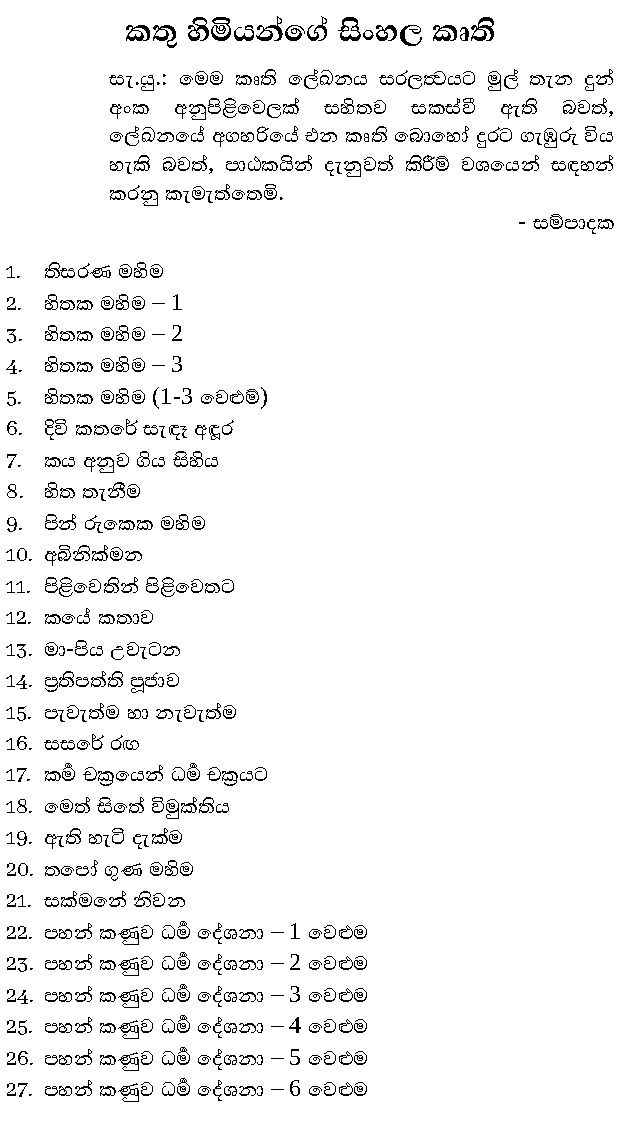
\includegraphics{sinhala-titles-p01.pdf}

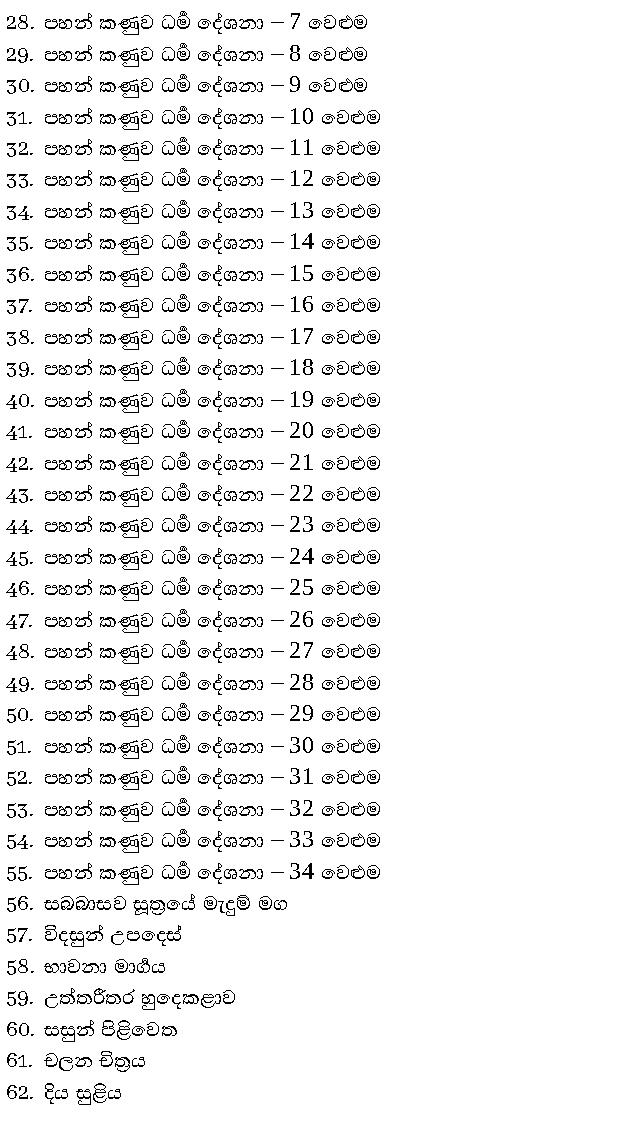
\includegraphics{sinhala-titles-p02.pdf}

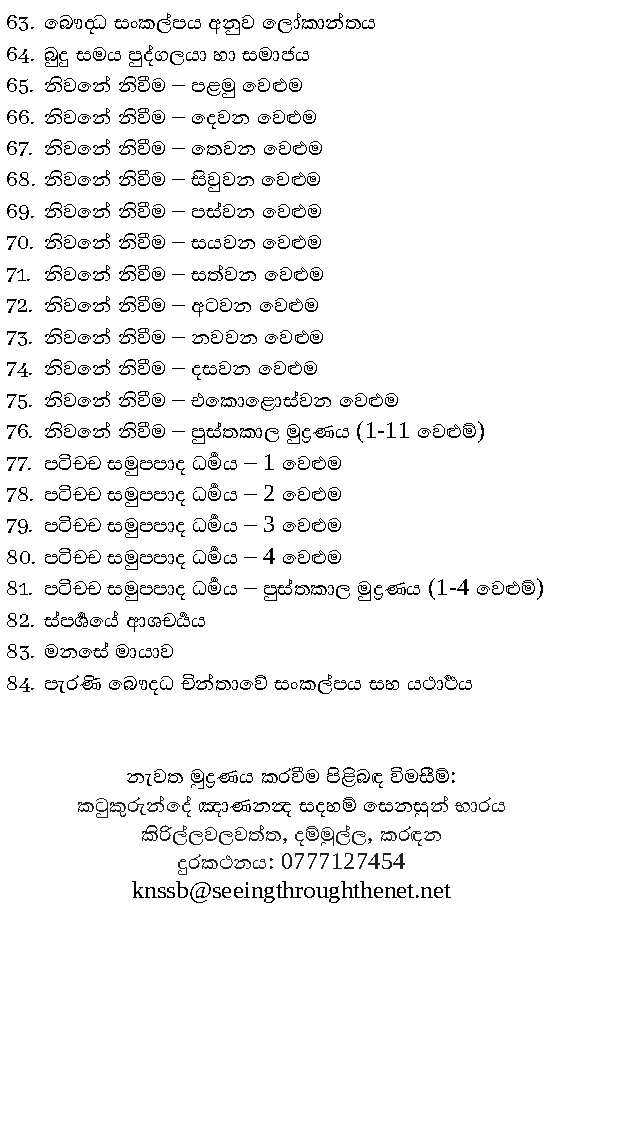
\includegraphics{sinhala-titles-p03.pdf}


\cleartorecto
\thispagestyle{plain}

{\fontsize{10}{14}\selectfont%
\setlength{\parindent}{0pt}%
\raggedright\label{copyright-details}%
\setlength{\parskip}{7pt}%

{\centering

{\LARGE\ccbyncnd}

This work is licensed under a Creative Commons\\
Attribution-NonCommercial-NoDerivatives 4.0 International~License.\footnote{%
\href{https://creativecommons.org/licenses/by-nc-nd/4.0/}{https://creativecommons.org/licenses/by-nc-nd/4.0/}}

}

You are free to:

\begin{packeditemize}
\item Share — copy and redistribute the material in any medium or format
\end{packeditemize}

The licensor cannot revoke these freedoms as long as you follow the license terms.

Under the following terms:

\begin{packeditemize}
\item Attribution — You must give appropriate credit, provide a link to the license, and indicate if changes were made. You may do so in any reasonable manner, but not in any way that suggests the licensor endorses you or your use.
\item NonCommercial — You may not use the material for commercial purposes.
\item NoDerivatives — If you remix, transform, or build upon the material, you may not distribute the modified material.
\end{packeditemize}

No additional restrictions — You may not apply legal terms or technological measures that legally restrict others from doing anything the license permits.

Notices:

You do not have to comply with the license for elements of the material in the public domain or where your use is permitted by an applicable exception or limitation.

No warranties are given. The license may not give you all of the permissions necessary for your intended use. For example, other rights such as publicity, privacy, or moral rights may limit how you use the material.

% TODO confirm this notice with The Publisher

\thePublisher\ asserts its moral right to be identified as the author of this book.

\thePublisher\ requests that you attribute ownership of the work to \thePublisher\ on copying, distribution, display or performance of the work.

}


\emptyUntilEven

\end{document}
